\documentclass[openright,twoside]{iitbthesis}
\usepackage{graphicx} % Required for inserting images
\usepackage{epsfig} 
\usepackage{amsmath} 
\usepackage{amssymb}  
\usepackage{circuitikz}
\usepackage{mathdots}
\usepackage[inline]{enumitem}                   
\usepackage{wrapfig}
\usepackage{booktabs}
\usepackage{multirow}
\usepackage{scalefnt}
\usepackage{multicol}
\usepackage{bm}
\usepackage{bbm}
\usepackage{dsfont}
\usepackage{nicematrix}
\usepackage{verbatim}
\usepackage{mathrsfs}
\usepackage{mathtools}
\usepackage{commands}
\usepackage{theorems}
\usepackage{environments}
\usepackage{longtable}
\usepackage{microtype}
\usepackage{tabularx}
\usepackage{array}
\usepackage{ragged2e}
\setlength{\emergencystretch}{2em}
%Tikz Settings for figures
\usepackage{tikz-cd}
\usepackage{tikz}
\usepackage{subcaption}
%\usepackage{subfigure}
\usetikzlibrary{arrows, matrix}
\usetikzlibrary{arrows.meta, angles, quotes, calc}
\usetikzlibrary{shapes, arrows, calc, arrows.meta, fit, positioning}%graphs,graphdrawing} %\usegdlibrary{layered}
\tikzset{  
-Latex,auto,node distance =2 cm and 1.3 cm, thick,% node distance is the distance between one node to other, where 1.5cm is the length of the edge between the nodes  
state/.style ={circle, draw, minimum width = 0.9 cm}, % the minimum width is the width of the ellipse, which is the size of the shape of vertex in the node graph  
point/.style = {circle, draw, inner sep=0.18cm, fill, node contents={}},  
dotteddirected/.style={-Latex,loosely dash dot}, % it is the edge having two directions  
reverseedge/.style={-Latex,dotted}, % it is the dashed directed edge
el/.style = {inner sep=2.5pt, align=right, sloped}  
}

\begin{document}
\include{0_prelude}
%\include{1_intro}
\chapter{Introduction}\label{ch:intro}
\section{Motivation and Background}
\subsection{Emergence of Networked Autonomous Systems}
Over the past two decades, multi-agent systems (MAS) have transitioned from theoretical abstractions to critical infrastructure across modern engineering domains. AI, especially agentic AI, Distributed vehicular platoons, unmanned aerial vehicle (UAV) swarms, robotic cooperative manipulation teams, and decentralized smart microgrids, all rely on distributed coordination algorithms. Compared to traditional centralized control architectures, distributed frameworks offer significant advantages:
\begin{itemize}
    \item \textbf{Scalability:} Computational load is distributed across individual agent nodes, avoiding exponential growth in processing overhead at a central server. 
    \item \textbf{Spatial Coverage and Flexibility:} Localized interaction topologies enable large - scale geographic deployment, allowing swarms to adapt to changing environments dynamically.
    \item \textbf{Fault Tolerance:} Eliminating single points of failure ensures that the loss or degradation of an individual node does not compromise the global mission.
\end{itemize}
A fundamental requirement in all multi-agent coordination problems is achieving consensus-- a state where a group of autonomous agents reaches agreement on a shared physical or virtual variable (such as position, velocity, heading, or phase) relying solely on local inter-agent communication.

\subsection{Topologies, Information Flow, and Graph Theory Fundamentals}
In networked multi-agent systems, the interaction structure among agents is modelled using graph theory \cite{godsil2001algebraic, mesbahi2010graph}. Let $\G = (\Vg, \Eg, \Wg)$ represent a weighted directed graph (digraph).
\begin{definition}[Weighted Directed Graph \cite{mesbahi2010graph, ren2008consensus}]\label{def:weighted_digraph}
A weighted directed graph (or digraph) is defined as a triplet $\G = (\Vg, \Eg, \Wg)$, where:
\begin{enumerate}
    \item $\Vg = \{1, 2, \dots, N\}$ is a finite, non-empty set of $N$ discrete nodes or vertices, with $N = |\Vg|$ representing the total number of autonomous agents in the network.
    \item $\Eg \subseteq \Vg \times \Vg$ is the set of directed edges (or arcs) representing directed information channels. An ordered pair $(j, i) \in \Eg$ denotes a directed edge originating at tail node $j$ and terminating at head node $i$. In this setup, information flows strictly from agent $j$ to agent $i$; node $j$ is classified as a parent/neighbor of node $i$, and node $i$ is classified as a child of node $j$. Self-loops are excluded, i.e., $(i, i) \notin \Eg, \forall i \in \Vg$.
    \item $\Wg = [w_{ij}] \in \R^{N \times N}$ is the weighted adjacency matrix. The matrix entry $w_{ij}$ represents the non-negative weight associated with the edge $(j, i) \in \Eg$:
    \begin{equation}\label{eq:adj_matrix_def}
        w_{ij} = \begin{cases}
            > 0, & \text{if } (j, i) \in \Eg \\
            0, & \text{otherwise}
        \end{cases}
    \end{equation}
    For an unweighted graph, $w_{ij} = 1$ whenever $(j, i) \in \Eg$.
\end{enumerate}
\end{definition}

\begin{definition}[Neighbor Sets and In-Degree Matrix \cite{ren2008consensus, mesbahi2010graph}]\label{def:neighbor_set}
The set of in - neighbors of agent $i$, denoted by $\mathcal{N}_i$, consists of all nodes from which agent $i$ receives direct state information:
\begin{equation}
    \mathcal{N}_i = \{j \in \Vg : (j, i) \in \Eg\}
\end{equation}
The weighted in-degree of node $i$, denoted by $d_{\text{in}, i}$, is the sum of the weights of all incoming edges to node $i$:
\begin{equation}
    d_{\text{in}, i} = \sum_{j \in \mathcal{N}_i} w_{ij} = \sum_{j=1}^{N} w_{ij}
\end{equation}
The network in-degree matrix $\Dg \in \R^{N \times N}$ is a diagonal matrix containing the in-degrees of all agents:
\begin{equation}\label{eq:indegree_matrix}
    \Dg = \text{diag}(d_{\text{in}, 1}, d_{\text{in}, 2}, \dots, d_{\text{in}, N})
\end{equation}
\end{definition}

\begin{definition}[Node Graph Laplacian Matrix \cite{godsil2001algebraic, mesbahi2010graph}]\label{def:ch_intro_graphLaplacian}
The node graph Laplacian matrix $\mathcal{L} \in \R^{N \times N}$ associated with the graph $\G$ is defined as:
\begin{equation}\label{eq:laplacian_def}
    \mathcal{L} = \Dg - \Wg
\end{equation}
where $\Dg = \text{diag}(d_{in,1}, d_{in,2}, \dots, d_{in,N})$ is the in-degree matrix with diagonal elements $d_{in,i} = \sum_{j=1}^{N} w_{ij}$.\\
Element-wise, the elements of the Laplacian matrix $[\mathcal{L}]_{ij} \eqqcolon l_{ij}$ are given by:
\begin{equation}\label{eq:ch_intro_laplacianentries}
    l_{ij} = \begin{cases}
        \sum_{k=1, k \neq i}^{N} w_{ik}, & \text{if } i = j \\
        -w_{ij}, & \text{if } i \neq j
    \end{cases}
\end{equation}
\end{definition}
\begin{remark}[Spectral Properties of the Laplacian \cite{ren2005second, mesbahi2010graph}]\label{prop:ch_intro_laplacianzeroeig}
\leavevmode\par\noindent
The graph Laplacian $\mathcal{L}$ exhibits the following fundamental spectral properties:
\begin{enumerate}
    \item \textbf{Row-Sum Property and Zero Eigenvalue:} By definition \eqref{eq:ch_intro_laplacianentries}, the sum of entries along every row of $\mathcal{L}$ is identically zero:
    \begin{equation}
        \sum_{j=1}^{N} l_{ij} = d_{\text{in}, i} - \sum_{j=1, j \neq i}^{N} w_{ij} = 0, \quad \forall i \in \{1, 2, \dots, N\}
    \end{equation}
    This establishes that $\mathcal{L} \mathbf{1}_N = 0_{N \times 1}$, where $\mathbf{1}_N = [1, 1, \dots, 1]^T \in \R^N$ is the vector of all ones. Thus, $\lambda_1 = 0$ is always an eigenvalue of $\mathcal{L}$ with a corresponding right eigenvector $\mathbf{1}_N$.
    
    \item \textbf{Positive Real Spectrum Location:} By Gershgorin's Disc Theorem, all eigenvalues $\lambda \in \sigma(\mathcal{L})$ lie within the union of closed discs centered at $l_{ii} = d_{\text{in},i}$ with radii $R_i = \sum_{j \neq i} |l_{ij}| = d_{\text{in},i}$. Consequently, every eigenvalue satisfies:
    \begin{equation}
        \mathfrak{Re}(\lambda_i) \ge 0, \quad \forall i \in \{1, 2, \dots, N\}
    \end{equation}
    
    \item \textbf{Strict Positivity of Non-Zero Eigenvalues:} If the directed graph $\G$ contains a \emph{directed spanning tree}, then $\lambda_1 = 0$ is a simple eigenvalue (algebraic multiplicity of one), and all remaining $N-1$ non-zero eigenvalues satisfy:
    \begin{equation}
        \mathfrak{Re}(\lambda_i) > 0, \quad \forall i \in \{2, 3, \dots, N\}
    \end{equation}
    ordered by real parts such that $0 = \lambda_1 < \mathfrak{Re}(\lambda_2) \le \dots \le \mathfrak{Re}(\lambda_N)$.
\end{enumerate}
\end{remark}
\subsubsection{Topological Connectivity and Graph Classifications (Directed Graphs)}
The stability and performance of multi-agent protocols depend directly on the structural connectivity of the underlying graph. 
\begin{definition}[Path, Cycle, and Connectivity \cite{godsil2001algebraic}]\label{def:paths_cycles}
\leavevmode\par\noindent
\begin{enumerate}
    \item A \emph{directed path} from node $i_0$ to node $i_k$ is a finite sequence of distinct nodes $(i_0, i_1, \dots, i_k)$ such that $(i_{m-1}, i_m) \in \Eg$ for all $m \in \{1, 2, \dots, k\}$.
    \item A \emph{directed cycle} (or loop) is a directed path that begins and ends at the same vertex, i.e., $i_0 = i_k$, with all intermediate nodes being distinct.
    \item A graph $\G$ is \emph{strongly connected} if there exists a directed path between every pair of distinct vertices $i, j \in \Vg$.
    \item A graph $\G$ contains a \emph{directed spanning tree} if there exists at least one node $r \in \Vg$ (termed the root or leader node) such that a directed path exists from $r$ to every other node $i \in \Vg \setminus \{r\}$. The root node has an in-degree of zero ($d_{\text{in}, r} = 0$) in an acyclic network.
\end{enumerate}
\end{definition}

\begin{definition}[Topological Ordering and Reverse Edges \cite{hao2019role} \cite{dubey2022consensus}]\label{def:topological_ordering}
A graph $\G$ admits a \emph{topological ordering} if its vertices can be indexed as $\{1, 2, \dots, N \}$ such that every directed edge $(j, i) \in \Eg$ satisfies $j < i$.
\begin{enumerate}
    \item Topological ordering is possible if and only if the directed graph $\G$ is acyclic (a Directed Acyclic Graph, or DAG).
    \item Under a topological ordering, the weighted adjacency matrix $\Wg$ and graph Laplacian $\mathcal{L}$ are strictly lower triangular.
    \item A \emph{reverse edge} is a directed edge $(y, x) \in \Eg$ that violates the topological ordering condition, i.e., $y > x$. Adding a reverse edge to an acyclic chain network creates a directed cycle.
    \item The \emph{cycle length} $\ell$ created by a reverse edge from tail node $y$ to head node $x$ is defined as:
    \begin{equation}\label{eq:cycle_length_def}
        \ell = y - x
    \end{equation}
    \begin{remark}
        Note that $\ell$ is defined as one less than the number of nodes participating in the cycle.
    \end{remark}
\end{enumerate}
\end{definition}
\subsubsection{Some Illustrative Numerical Examples}
To illustrate some of these concepts, consider two distinct 5-agent topologies ($N = 5$) with unit edge weights.
\begin{example}[Acyclic Directed Chain with Topological Ordering]\label{example:acyclic_chain_ex}
Consider a 5 agents directed chain as in Figure \ref{fig:acyclic_chain_ex}, where, information flows strictly downstream from Node 1 to Node 5.

\begin{figure}[ht!]
    \centering
    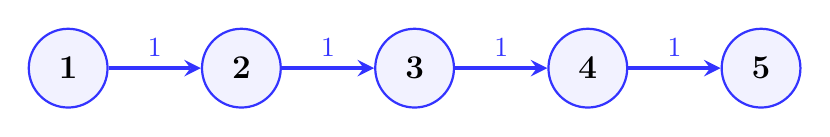
\begin{tikzpicture}[node distance=2.2cm, state/.style={circle, draw=blue!80, fill=blue!5, thick, minimum size=1.0cm, font=\large\bfseries}]
        \node[state] (1) {1};
        \node[state] (2) [right of=1] {2};
        \node[state] (3) [right of=2] {3};
        \node[state] (4) [right of=3] {4};
        \node[state] (5) [right of=4] {5};
        
        \path [->, >=stealth, ultra thick, blue!80] (1) edge node[above] {$1$} (2);
        \path [->, >=stealth, ultra thick, blue!80] (2) edge node[above] {$1$} (3);
        \path [->, >=stealth, ultra thick, blue!80] (3) edge node[above] {$1$} (4);
        \path [->, >=stealth, ultra thick, blue!80] (4) edge node[above] {$1$} (5);
    \end{tikzpicture}
    \caption{A 5-agent directed chain topology with topological ordering.}
    \label{fig:acyclic_chain_ex}
\end{figure}

The adjacency matrix $\mathcal{W}_{\mathcal{G}1}$, in-degree matrix $\mathcal{D}_{\mathcal{G}1}$, and Laplacian matrix $\mathcal{L}_{\mathcal{G}1}$ for this topology are:
\begin{equation*}
\mathcal{W}_{\mathcal{G}1} = \begin{bmatrix} 
0 & 0 & 0 & 0 & 0 \\ 
1 & 0 & 0 & 0 & 0 \\ 
0 & 1 & 0 & 0 & 0 \\ 
0 & 0 & 1 & 0 & 0 \\ 
0 & 0 & 0 & 1 & 0 
\end{bmatrix}, \quad
\mathcal{D}_{\mathcal{G}1} = \text{diag}(0, 1, 1, 1, 1), \quad
\mathcal{L}_{\mathcal{G}1} = \begin{bmatrix} 
0 & 0 & 0 & 0 & 0 \\ 
-1 & 1 & 0 & 0 & 0 \\ 
0 & -1 & 1 & 0 & 0 \\ 
0 & 0 & -1 & 1 & 0 \\ 
0 & 0 & 0 & -1 & 1 
\end{bmatrix}
\end{equation*}
Since $\mathcal{L}_{\mathcal{G}1}$ is strictly lower triangular, its eigenvalues are $\sigma(\mathcal{L}_{\mathcal{G}1}) = \{0, 1, 1, 1, 1\}$. The spectrum is entirely real, with a simple eigenvalue at zero corresponding to the root node (Node 1).
\end{example}

\begin{example}[Directed Chain with a Reverse Edge Forming a Cycle]\label{example:cyclic_chain_ex}
\leavevmode\par \noindent
Now consider the graph shown in Figure \ref{fig:cyclic_chain_ex}, formed by adding a reverse edge from Node 4 to Node 2 ($y = 4, x = 2$) to the chain in Example \ref{example:acyclic_chain_ex}. This creates a directed cycle of length $\ell = 4 - 2 = 2$ involving nodes $\{2, 3, 4\}$.

\begin{figure}[ht!]
    \centering
    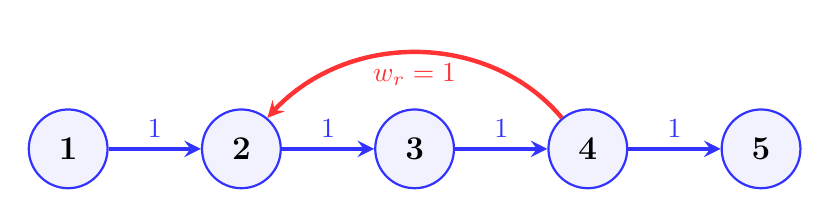
\begin{tikzpicture}[node distance=2.2cm, state/.style={circle, draw=blue!80, fill=blue!5, thick, minimum size=1.0cm, font=\large\bfseries}]
        \node[state] (1) {1};
        \node[state] (2) [right of=1] {2};
        \node[state] (3) [right of=2] {3};
        \node[state] (4) [right of=3] {4};
        \node[state] (5) [right of=4] {5};
        
        \path [->, >=stealth, ultra thick, blue!80] (1) edge node[above] {$1$} (2);
        \path [->, >=stealth, ultra thick, blue!80] (2) edge node[above] {$1$} (3);
        \path [->, >=stealth, ultra thick, blue!80] (3) edge node[above] {$1$} (4);
        \path [->, >=stealth, ultra thick, blue!80] (4) edge node[above] {$1$} (5);
        \path [->, >=stealth, ultra thick, red!80] (4) edge[bend right=50] node[below] {$w_r = 1$} (2);
    \end{tikzpicture}
    \caption{A 5-agent directed chain with a reverse edge $(4, 2)$ forming a directed cycle of length $\ell = 2$.}
    \label{fig:cyclic_chain_ex}
\end{figure}

The modified adjacency matrix $\mathcal{W}_{\mathcal{G}2}$ and Laplacian matrix $\mathcal{L}_{\mathcal{G}2}$ are:
\begin{equation*}
\mathcal{W}_{\mathcal{G}2} = \begin{bmatrix} 
0 & 0 & 0 & 0 & 0 \\ 
1 & 0 & 0 & 1 & 0 \\ 
0 & 1 & 0 & 0 & 0 \\ 
0 & 0 & 1 & 0 & 0 \\ 
0 & 0 & 0 & 1 & 0 
\end{bmatrix}, \quad
\mathcal{L}_{\mathcal{G}2} = \begin{bmatrix} 
0 & 0 & 0 & 0 & 0 \\ 
-1 & 2 & 0 & -1 & 0 \\ 
0 & -1 & 1 & 0 & 0 \\ 
0 & 0 & -1 & 1 & 0 \\ 
0 & 0 & 0 & -1 & 1 
\end{bmatrix}
\end{equation*}
Computing the characteristic equation $|\lambda I_5 - \mathcal{L}_{\mathcal{G}2}| = \lambda (\lambda - 1) [(\lambda - 2)(\lambda - 1)^2 - 1] = 0$ yields the Laplacian eigenvalues:
\begin{equation*}
\sigma(\mathcal{L}_{\mathcal{G}2}) = \left\{ 0, \; 1, \; 2.4656, \; 0.7672 + j 0.7925, \; 0.7672 - j 0.7925 \right\}
\end{equation*}
The addition of the reverse edge introduces a pair of complex-conjugate eigenvalues with imaginary parts $\mathfrak{Im}(\lambda) = \pm 0.7925$.
\end{example}

\subsubsection{Dynamical Agent Models and Kronecker Products as a useful tool}
The interaction topology modeled by $\G$ dictates the state evolution of physical agents. In this dissertation, we analyze agents with second-order (double-integrator) dynamics.

Consider $N$ double-integrator agents operating in $d$-dimensional space ($d \in \{1, 2, 3\}$):
\begin{equation}\label{eq:double_integrator_model}
    \dot{p}_i(t) = v_i(t), \quad \dot{v}_i(t) = u_i(t), \quad i \in \{1, 2, \dots, N\}
\end{equation}
where $p_i(t) = [p_{i,1}, \dots, p_{i,d}]^T \in \R^d$ and $v_i(t) = [v_{i,1}, \dots, v_{i,d}]^T \in \R^d$ denote the position and velocity vectors of agent $i$, and $u_i(t) \in \R^d$ denotes its acceleration control input.

The distributed consensus control law as proposed by \cite{ren2005second} and \cite{ren2008consensus} is:
\begin{equation}\label{eq:consensus_control_law_local}
    u_i(t) = -\sum_{j=1}^{N} w_{ij} \left[ \left( p_i(t) - p_j(t) \right) + \gamma \left( v_i(t) - v_j(t) \right) \right]
\end{equation}
where $\gamma > 0$ is the global velocity coupling parameter.

Stacking the network position and velocity vectors into $p(t) = [p_1^T(t), \dots, p_N^T(t)]^T \in \R^{Nd}$ and $v(t) = [v_1^T(t), \dots, v_N^T(t)]^T \in \R^{Nd}$, the control protocol \eqref{eq:consensus_control_law_local} can be expressed compactly using the Kronecker product $\otimes$:
\begin{equation}\label{eq:network_dynamics_kronecker}
    \begin{aligned}
        \dot{p}(t) &= v(t) \\
        \dot{v}(t) &= -(\mathcal{L} \otimes I_d) p(t) - \gamma (\mathcal{L} \otimes I_d) v(t)
    \end{aligned}
\end{equation}

Defining the composite state vector $\mathcal{X}(t) := [p^T(t), v^T(t)]^T \in \R^{2Nd}$, the network state-space representation is:
\begin{equation}\label{eq:composite_state_space}
    \dot{\mathcal{X}}(t) = (\hat{\mathcal{L}} \otimes I_d) \mathcal{X}(t), \quad \text{where } \hat{\mathcal{L}} = \begin{bmatrix} 0_{N,N} & I_N \\ -\mathcal{L} & -\gamma \mathcal{L} \end{bmatrix} \in \R^{2N \times 2N}
\end{equation}
where $0_{N,N}$ and $I_N$ represent the $N \times N$ zero and identity matrices, respectively.

\subsubsection{Gershgorin's Disc Theorem}

To bound Laplacian eigenvalues and ensure stability without explicitly factoring high-order characteristic polynomials, Gershgorin's Disc Theorem serves as a primary tool.

\begin{theo}[Gershgorin's Disc Theorem \cite{horn2012matrix}]\label{thm:gershgorin_detailed}
Let $A = [a_{ij}] \in \R^{n \times n}$ be a square matrix. For each column $j \in \{1, 2, \dots, n\}$, define the column-sum radius $R_j(A)$ as the sum of the absolute values of the non-diagonal elements in column $j$:
\begin{equation}\label{eq:gershgorin_radius}
    R_j(A) = \sum_{i=1, i \neq j}^{n} |a_{ij}|
\end{equation}
Associated with each column $j$, define a closed disk $\mathfrak{D}_j(A)$ in the complex plane $\mb{C}$, centered at the diagonal entry $a_{jj}$ with radius $R_j(A)$:
\begin{equation}\label{eq:gershgorin_disc}
    \mathfrak{D}_j(A) = \left\{ z \in \mb{C} : |z - a_{jj}| \le R_j(A) \right\}
\end{equation}
Then, all eigenvalues $\lambda \in \sigma(A)$ lie within the union of these $n$ Gershgorin discs:
\begin{equation}
    \sigma(A) \subset D(A) \coloneqq \bigcup_{j=1}^{n} \mathfrak{D}_j(A)
\end{equation}
Since $\sigma(A) = \sigma(A^T)$, identical statements hold using row-sum radii.
\end{theo}

\begin{figure}[ht!]
    \centering
    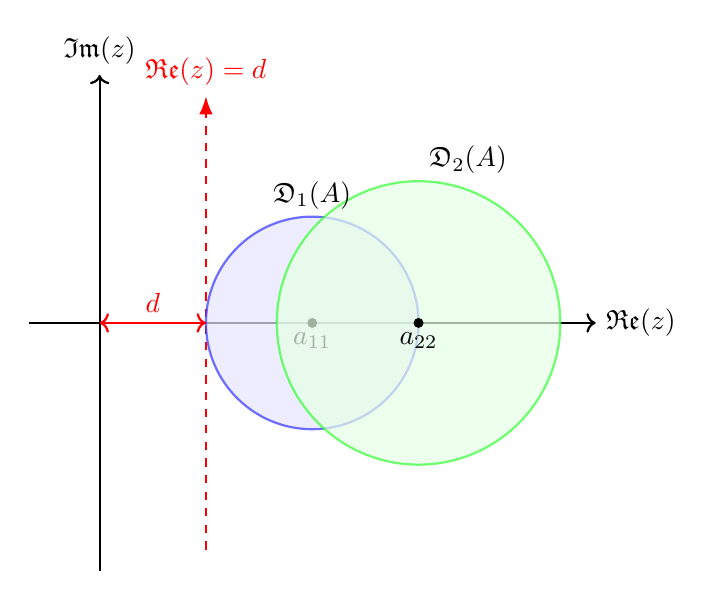
\begin{tikzpicture}[scale=0.9]
        % Axes
        \draw[->, thick] (-1,0) -- (7,0) node[right] {$\mathfrak{Re}(z)$};
        \draw[->, thick] (0,-3.5) -- (0,3.5) node[above] {$\mathfrak{Im}(z)$};
        
        % Vertical distance line
        \draw[dashed, red, thick] (1.5,-3.2) -- (1.5,3.2) node[above] {$\mathfrak{Re}(z) = d$};
        
        % Discs
        \draw[fill=blue!10, draw=blue!80, thick, opacity=0.7] (3.0,0) circle (1.5cm);
        \fill (3.0,0) circle (2pt) node[below] {$a_{11}$};
        
        \draw[fill=green!10, draw=green!80, thick, opacity=0.7] (4.5,0) circle (2.0cm);
        \fill (4.5,0) circle (2pt) node[below] {$a_{22}$};
        
        % Annotations
        \draw[<->, thick, red] (0,0) -- (1.5,0) node[midway, above] {$d$};
        \node at (3.0, 1.8) {$\mathfrak{D}_1(A)$};
        \node at (5.2, 2.3) {$\mathfrak{D}_2(A)$};
    \end{tikzpicture}
    \caption{Geometric illustration of Gershgorin discs bounded away from the origin by a minimum real separation distance $d > 0$.}
    \label{fig:gershgorin_concept}
\end{figure}

In Chapter 3, Gershgorin's Disc Theorem is applied to shift matrix sub-blocks to design local node and edge perturbation factors that enforce a minimal separation distance $d \ge 1/\gamma^2$  of the non-zero eigenvalue of the Laplacian with the smallest real part from the imaginary axis, thereby guaranteeing second-order consensus.

\subsubsection{The Ramifications of Feedback Cycles in Networks}
A foundational result in consensus theory states that a networked system can achieve state agreement over a directed graph if and only if the communication topology $\mathcal{G}$ contains a directed spanning tree (a rooted out-branching)— a subgraph where at least one node (the root or leader node) has a directed path to every other node in the network. 

In physical networks, directed cycles (or feedback loops) arise naturally due to bidirectional spatial proximity, feedback mechanisms between lower and higher organizational tiers, or reverse-edge communication channels. For example, in an autonomous vehicular platoon moving over a directed chain topology, information primarily flows downstream (vehicle $i-1$ to vehicle $i$). However, if a downstream vehicle transmits spatial coordinates back to an upstream vehicle to enforce tight inter-vehicular spacing, a closed directed cycle is formed. Directed loops present a critical dichotomy in multi-agent networks:
\begin{itemize}
    \item \textbf{The Single-Integrator Case:} For first-order networks, the introduction of reverse edges leading to directed cycles merely degrades the algebraic connectivity (Fiedler eigenvalue) and slows down the rate of convergence to consensus, without jeopardizing consensus altogether.
    \item \textbf{The Double-Integrator Case:} For second-order networks, directed cycles introduce complex-conjugate eigenvalues with imaginary components into the graph Laplacian spectrum. These complex eigenvalues induce phase lag between position alignment and velocity damping. If the velocity coupling parameter $\gamma$ falls below a critical lower bound, this phase lag can cause severe dynamic instability, leading to complete breakdown of consensus despite the presence of a directed spanning tree.
\end{itemize}

\subsection{Incidence Matrices, Edge Factorizations, and Tree Decompositions}
To enable disturbance attenuation and $\mathcal{H}_2$ norm analysis (as developed in Chapter \ref{ch:Robustness_Analysis}), we consider a network of double-integrator agents operating over an undirected path graph. For an effective $\mathcal{H}_2$ performance evaluation, the network dynamics are more conveniently expressed using edge-based state representations rather than traditional node-based coordinates. This transformation isolates and eliminates the zero eigenvalue of the graph Laplacian, thereby yielding a non-singular, reduced-order Laplacian structure required for internal stability and transfer function formulation. A non-singular structure is needed to ensure the state matrix $\mathcal{A}_x$ is Hurwitz, allowing the computation of controllability/observability Gramians and the transfer function $G(s) = \mathcal{C}_z(sI - \mathcal{A}_x)^{-1}\mathcal{B}_w$.

A comprehensive treatment of the graph-theoretic definitions and edge-space formulations presented in this section can be found in \cite{zelazo2007agreement, zelazo2009h2, zelazo2010edge}.

Let $e = |\Eg|$ denote the total number of edges in the graph $\G$. Assign an arbitrary orientation index $k \in \{1, 2, \dots, e\}$ to each edge $(j, i) \in \Eg$.

\begin{definition}[Incidence Matrix]\label{def:incidence_matrix}
The node-edge incidence matrix $E(\G) \in \R^{N \times e}$ of an undirected graph $\G$ has its $(i, k)$-th entry defined as:
\begin{equation}
    [E(\G)]_{ik} = \begin{cases}
        +1, & \text{if vertex } i \text{ is the head (destination) of directed edge } k \\
        -1, & \text{if vertex } i \text{ is the tail (source) of directed edge } k \\
        0, & \text{otherwise}
    \end{cases}
\end{equation}
For an unweighted undirected graph, the relationship between the node Laplacian $\mathcal{L}$ and the incidence matrix $E(\G)$ is given by:
\begin{equation}
    \mathcal{L} = E(\G) E(\G)^T
\end{equation}
The edge Laplacian matrix $\mathcal{L}_e \in \R^{e \times e}$ is defined dually as:
\begin{equation}
    \mathcal{L}_e = E(\G)^T E(\G)
\end{equation}
\end{definition}
\begin{definition}[Spanning Tree Factorization of the Incidence Matrix] \label{def:spanning_tree_factorization}
\leavevmode\par\noindent
Consider a graph $\G$ containing a spanning tree. By topological reordering of the edge columns, the incidence matrix $E(\G)$ can be partitioned into tree edges and cycle-closing edges:
\begin{equation}
    E(\G) = \begin{bmatrix} \etree & E_c \end{bmatrix}
\end{equation}
where $\etree \in \R^{N \times (N-1)}$ represents the $N-1$ columns belonging to a chosen spanning tree, and $E_c \in \R^{N \times (e - N + 1)}$ represents the remaining $e - N + 1$ edges that form cycles.
Since the columns of $E_c$ lie in the column space spanned by $\etree$, there exists a linear transformation matrix $T \in \R^{(N-1) \times (e - N + 1)}$ such that $E_c = \etree T$. The transformation matrix $T$ is given by:
\begin{equation}
    T = (\etree^T \etree)^{-1} \etree^T E_c
\end{equation}
Thus, the full incidence matrix can be factored compactly as:
\begin{equation}\label{eq:incidence_factored}
    E(\G) = \etree \begin{bmatrix} I_{N-1} & T \end{bmatrix} =: \etree R
\end{equation}
where $R := \begin{bmatrix} I_{N-1} & T \end{bmatrix} \in \R^{(N-1) \times e}$.

The reduced tree node Laplacian $\lntree$ and reduced tree edge Laplacian $\letree$ are defined respectively as:
\begin{equation}
    \lntree = \etree \etree^T \in \R^{N \times N}, \quad \letree = \etree^T \etree \in \R^{(N-1) \times (N-1)}
\end{equation}
\end{definition}

\subsubsection{System Performance via the $\mathcal{H}_2$ Norm}
To measure noise propagation and disturbance rejection in second-order agent networks under process noise $q(t) \in \R^N$ and measurement noise $r(t) \in \R^e$, we use the $\mathcal{H}_2$ norm metric.

Consider a stable, linear time-invariant (LTI) reduced-order system $\Sigma_e$ expressed in edge coordinates:
\begin{equation}\label{eq:h2_system_def}
    \begin{aligned}
        \dot{x}_e(t) &= \mathcal{A}_x x_e(t) + \mathcal{B}_w w(t) \\
        z(t) &= \mathcal{C}_z x_e(t)
    \end{aligned}
\end{equation}
where $w(t) = [q^T(t), r^T(t)]^T$ is a vector of uncorrelated zero-mean Gaussian white noise processes, $x_e(t)$ represents relative edge states, and $z(t)$ denotes regulated output errors.

When $\mathcal{A}_x$ is Hurwitz, the squared $\mathcal{H}_2$ norm of the system transfer function $G(s) = \mathcal{C}_z (s I - \mathcal{A}_x)^{-1} \mathcal{B}_w$ is given by \cite{dullerud2013course}:
\begin{equation}\label{eq:h2_norm_trace}
    \|\Sigma_e\|_{\mathcal{H}_2}^2 = \text{trace}(\mathcal{C}_z \mathcal{P}_{\text{ctrl}} \mathcal{C}_z^T) = \text{trace}(\mathcal{B}_w^T \mathcal{P}_{\text{obs}} \mathcal{B}_w)
\end{equation}
where $\mathcal{P}_{\text{ctrl}}$ and $\mathcal{P}_{\text{obs}}$ are the controllability and observability Gramians, satisfying the Lyapunov equations:
\begin{equation}\label{eq:lyapunov_equations}
    \mathcal{A}_x \mathcal{P}_{\text{ctrl}} + \mathcal{P}_{\text{ctrl}} \mathcal{A}_x^T + \mathcal{B}_w \mathcal{B}_w^T = 0_{2(N-1), 2(N-1)}
\end{equation}
\begin{equation}
    \mathcal{A}_x^T \mathcal{P}_{\text{obs}} + \mathcal{P}_{\text{obs}} \mathcal{A}_x + \mathcal{C}_z^T \mathcal{C}_z = 0_{2(N-1), 2(N-1)}
\end{equation}

In Chapter 4, closed-form solutions for $\|\Sigma_e\|_{\mathcal{H}_2}^2$ are derived to establish how graph cycle length, spatial loop placement relative to the root node, and dual-loop overlap govern stochastic noise attenuation.


\subsection{Real-World Applications: Cooperative Guidance and Interception}
The theoretical analysis and synthesis of consensus protocols is directly connected to physical motion control in defense and aerospace engineering, specifically in coordinated interception and cooperative multi-agent guidance. In modern precision strike missions against stationary or low-maneuverability targets (such as naval vessels or ground installations), a single interceptor can be countered by Close-In Weapon Systems (CIWS).

To overcome such defensive countermeasures, swarms of autonomous interceptors need to execute coordinated attacks. This requires solving two physical constraints simultaneously:
\begin{itemize}
    \item Temporal Constraint (Impact Time $t_{\text{imp}}$): All interceptors in the swarm must intercept the target at the exact same time instant to overwhelm automated defenses.
    \item Directional Constraint (Impact Angle $\zeta$): Each interceptor must intercept the target along a designated approach angle to maximize warhead penetration or exploit blind spots of the target's radar system.
\end{itemize}
Executing these cooperative engagements under strict non-holonomic kinematics and actuator limits ($\vert{}a_M\vert{} \le a^{\text{max}}$) requires bridging the ideas of consensus theory with physical trajectory generation for individual interceptors.

\section{Research Context and Problem Overview}
The research presented in this dissertation addresses four interconnected problems arising in networked dynamical systems and autonomous multi-agent coordination.
\begin{enumerate}
    \item \textbf{Consensus Stability over Directed Cyclic Networks:} The introduction of reverse communication edges in directed
    chain networks modifies the Laplacian spectrum and can compromise consensus stability in double-integrator systems.
    Understanding the influence of interacting directed cycles and developing suitable stability conditions are therefore
    important.
    \item \textbf{Decentralized Consensus Restoration:} In practical networks, the velocity coupling parameter may be fixed by design. Consequently, structural modifications should not necessarily require global spectral information or network-wide gain retuning. This motivates the development
    of localized strategies for restoring consensus.
    \item \textbf{Disturbance Attenuation and Network Performance:} In addition to stability, networked systems must maintain
    satisfactory performance in the presence of process and measurement disturbances. The relationship between directed cycle structure and the $\mathcal{H}_2$ performance of double-integrator networks requires investigation.
    \item \textbf{Constrained Trajectory Synthesis and Cooperative Interception:} Autonomous interceptors must satisfy terminal impact-angle and impact-time requirements while respecting physical acceleration constraints. Extending feasible trajectory synthesis to coordinated multi-agent systems introduces additional spatial and temporal coordination requirements.
\end{enumerate}
\section{Literature Review, Research Gaps and Problem Formulation} \label{sec:literature_review}

The research presented in this dissertation lies at the intersection of control theory, algebraic graph theory, networked dynamical systems, and autonomous guidance. This section reviews the relevant state-of-the-art across these domains and identifies the limitations that motivate the present research. Rather than treating the literature review and problem statements independently, each subsection discusses the existing developments, highlights the associated research gaps, and formulates the corresponding problem addressed in this dissertation.

\subsection{Consensus Protocols and Stability of Double-Integrator Networks}
\label{subsec:second_order_consensus}

The systematic study of consensus protocols, in which a group of autonomous agents achieves agreement on a common state through localized interactions, began with foundational works on first-order (single-integrator) systems \cite{saber2003consensus, jadbabaie2003coordination, fax2004information, 1333204}. Olfati-Saber and Murray \cite{saber2003consensus} established a graph-theoretic framework for consensus over fixed and switching communication topologies. Moreau \cite{moreau2005stability} subsequently extended these results to time-dependent directed communication links using set-valued Lyapunov functions.

While these foundational results primarily considered first-order agent dynamics, physical robotic platforms, UAVs, and mechanical systems are often governed by double-integrator dynamics, in which acceleration or force acts as the control input. Ren and Atkins \cite{ren2005second} extended consensus protocols to double-integrator agents over directed communication topologies. Consider $N$ double-integrator agents operating under the distributed control law
\begin{equation}
\label{eq:agent-wise}
    u_i(t) = -\sum_{j=1}^{N} w_{ij}
    \left[
    (p_i(t)-p_j(t))+
    \gamma(v_i(t)-v_j(t))
    \right],
    \quad i\in\{1,2,\ldots,N\},
\end{equation}
where $p_i(t),v_i(t)\in\mathbb{R}^d$ denote the position and velocity vectors of agent $i$, respectively, $w_{ij}$ is the $(i,j)$-th entry of the weighted adjacency matrix $\mathcal{W}$, and $\gamma>0$ is the velocity coupling parameter.

A fundamental distinction between first-order and second-order consensus emerges in directed networks. For first-order systems, the existence of a directed spanning tree is sufficient to guarantee consensus under the standard assumptions. In contrast, for double-integrator systems, the existence of a directed spanning tree alone does not guarantee consensus. The presence of complex Laplacian eigenvalues can introduce additional stability constraints, making consensus dependent on the choice of the velocity coupling parameter.

Ren and Atkins \cite{ren2005second} established a conservative sufficient lower bound on $\gamma$ for achieving consensus over general directed graphs containing a directed spanning tree:
\begin{equation}
\label{eq:ren_gamma_bound}
    \gamma >
    \max_{i\in\{2,\ldots,N\}}
    \sqrt{\frac{2}{\mathfrak{Re}(\lambda_i)}},
\end{equation}
where $\lambda_i$ denotes the $i$-th non-zero eigenvalue of the graph Laplacian matrix $\mathcal{L}$, ordered according to their real parts such that
$0=\lambda_1$ and
$0<\mathfrak{Re}(\lambda_2)\leq\cdots\leq\mathfrak{Re}(\lambda_N)$.

Subsequently, Yu et al. \cite{yu2009second, yu2010some} derived the exact necessary and sufficient condition for second-order consensus over directed topologies. According to their result, the velocity coupling parameter must satisfy
\begin{equation}
\label{eq:yu_gamma_exact_bound}
    \gamma >
    \max_{i\in\{2,\ldots,N\}}
    \frac{|\mathfrak{Im}(\lambda_i)|}{|\lambda_i|}
    \sqrt{\frac{1}{\mathfrak{Re}(\lambda_i)}},
\end{equation}
where
\[
    |\lambda_i|=
    \sqrt{
    \mathfrak{Re}(\lambda_i)^2+
    \mathfrak{Im}(\lambda_i)^2
    }
\]
is the magnitude of the $i$-th Laplacian eigenvalue. This condition establishes that the stability of double-integrator consensus depends on both the real and imaginary components of the Laplacian spectrum.

For acyclic directed networks, such as directed chains and trees, the Laplacian eigenvalues are real. Consequently, the right-hand side of \eqref{eq:yu_gamma_exact_bound} becomes zero, permitting consensus for any $\gamma>0$. The introduction of reverse communication edges, however, can create directed cycles and introduce complex-conjugate eigenvalue pairs. In such cases, the velocity coupling parameter must exceed a strictly positive threshold determined by the Laplacian spectrum.

Figures~\ref{fig:spanning_tree_consensus} and~\ref{fig:cycle_consensus_failure} illustrate this distinction. While consensus is achieved over an acyclic directed spanning-tree topology for the selected value of $\gamma$, the introduction of directed cycles can lead to a breakdown of consensus when the prescribed coupling parameter is insufficient.

\begin{figure}[ht!]
    \centering
    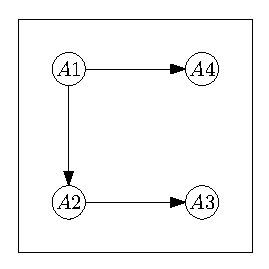
\includegraphics[width=0.6\textwidth,keepaspectratio]{Sapnning.eps}
    \caption{Consensus achieved for $\gamma=0.1$ over an acyclic directed spanning-tree topology.}
    \label{fig:spanning_tree_consensus}
\end{figure}

\begin{figure}[ht!]
    \centering
    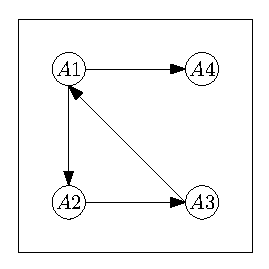
\includegraphics[width=0.6\textwidth,keepaspectratio]{Cycle.eps}
    \caption{Breakdown of consensus in the presence of directed cycles for an insufficient velocity coupling parameter.}
    \label{fig:cycle_consensus_failure}
\end{figure}

These results highlight an important limitation of existing consensus protocols. Although the analytical conditions in \eqref{eq:ren_gamma_bound} and \eqref{eq:yu_gamma_exact_bound} characterize the required velocity coupling, their application following a structural modification of the network may necessitate updated spectral information and a corresponding retuning of $\gamma$. In practical networks, however, the velocity coupling parameter may already be fixed by design, and global spectral information may not be available to individual agents.

This motivates the following research problem:
\begin{problem}
\label{prob:multi_loop_coupling}
Analyze how the presence of multiple interacting directed loops, whether disjoint, overlapping, or sharing root/leader nodes, modifies the Laplacian spectrum and the corresponding stability requirements for double-integrator consensus over directed chain topologies. Furthermore, develop localized edge and node perturbation strategies that guarantee consensus under a fixed, predesigned velocity coupling parameter, without requiring global spectral information or network-wide gain retuning.
\end{problem}

\subsection{Spectral Analysis of Directed Cycles and Decentralized Consensus Restoration}
\label{subsec:cyclic_spectral_analysis}

Feedback loops and directed cycles occur naturally in networked physical systems due to bidirectional communication links, spatial proximity, and multi-tiered communication architectures. Their influence on consensus has been investigated extensively, particularly in the context of first-order systems.

For single-integrator networks, the spectral properties of directed graphs and cyclic topologies have been studied from several perspectives \cite{mukherjee2016consensus, mukherjee2013reachability, mukherjee2021finite}. Zhang et al. \cite{zhang2017effect} analyzed the effect of adding a reverse edge across a stem in a directed acyclic graph (DAG), showing that the resulting convergence characteristics are governed by the subgraph encompassing the directed cycle. Mo et al. \cite{mo2019effects} extended this analysis to reverse edges across stems in DAGs.

For chain networks containing two reverse edges, Hao et al. \cite{hao2019role} investigated the dominant convergence root of single-integrator consensus and developed polynomial equations to characterize eigenvalue shifts. However, their analytical framework is subject to specific topological restrictions. In particular, the derivations are valid only when the lengths of the two cycles induced by the reverse edges differ by at least one, i.e.,
$|l_1-l_2|\geq 1$, and when the longer cycle is located strictly closer to the root node.

Although these studies provide useful insights into the influence of directed cycles on first-order consensus, the stability implications are fundamentally different for double-integrator systems. As discussed in Section~\ref{subsec:second_order_consensus}, complex Laplacian eigenvalues impose additional restrictions on the velocity coupling parameter. Therefore, characterizing the spectral effects of interacting directed cycles is essential for understanding and restoring consensus in second-order networks.

In particular, when the network contains multiple reverse edges, the resulting cycles may be disjoint, nested, or partially overlapping. Their interaction can modify the Laplacian spectrum in ways that are not captured by analyses restricted to a single cycle or to specific relative cycle lengths. Moreover, the need to restore consensus without changing a globally prescribed velocity coupling parameter motivates the development of localized node and edge perturbation strategies.

Accordingly, the research problem formulated in Problem~\ref{prob:multi_loop_coupling} also addresses the analytical characterization of interacting cycles and the development of decentralized consensus-restoration methodologies.

\subsection{Root-Node Loops and Structural Singularity}
\label{subsec:root_node_loop}

An additional difficulty arises when a reverse communication edge enters the root node itself. Conventional polynomial-based spectral analysis techniques, often exploit the hierarchical structure of a directed chain in which the root node has zero in-degree, i.e., $d_{\mathrm{in},1}=0$. Under this condition, the root node acts as an autonomous leader that is unaffected by downstream feedback.

When a reverse edge enters the root node itself ($x_1=1$), this hierarchical structure is no longer preserved. The root node acquires a nonzero in-degree, and the conventional leader-follower decomposition becomes inapplicable. In the particular cyclic configurations considered in this dissertation, the nodes within the directed cycle can no longer be treated using the original root-based hierarchy.

The analysis in \cite{hao2019role} also encounters this difficulty. When the root node participates in the cycle, the polynomial spectral methods yield trivial solutions, such as $s_1=1$, and fail to provide conclusive stability bounds. Thus, the existing polynomial framework does not resolve the consensus problem for this class of root-node loop configurations.

This leads to a distinct research problem:
\begin{problem}
When the root/leader node participates in a directed loop, the loss of its zero in-degree property invalidates the conventional root-based polynomial analysis and may lead to trivial characteristic solutions. Develop an analytical framework to characterize consensus stability in such configurations and formulate a decentralized strategy for restoring consensus without requiring global Laplacian spectral information or retuning the global velocity coupling parameter $\gamma$.
\end{problem}

\subsection{$\mathcal{H}_2$ Performance and Disturbance Attenuation in Cyclic Topologies}
\label{subsec:h2_performance}

Beyond deterministic convergence, real-world multi-agent networks operate in the presence of environmental disturbances, process noise, and sensor measurement errors. The $\mathcal{H}_2$ norm provides a measure of the total transient energy and stochastic disturbance amplification from exogenous inputs to network state deviations. Consequently, analyzing $\mathcal{H}_2$ performance is important not only for ensuring consensus but also for evaluating the quality of the resulting network response.

For single-integrator networks, Zelazo and Mesbahi \cite{zelazo2010edge} developed an edge-agreement framework based on the edge Laplacian, enabling a reduced-order representation of network dynamics by eliminating the zero Laplacian eigenvalue. Zelazo et al. \cite{zelazo2013performance} subsequently used this framework to analyze the $\mathcal{H}_2$ performance of single-integrator networks over cyclic graphs. Their results established that the performance depends on cycle length and is invariant to the choice of spanning tree and the spatial location of the cycle.

The performance of second-order networks under update delays and spectral variations has also been investigated by Huang and Siami \cite{huang2022role} and Oral et al. \cite{oral2017performance}. However, the $\mathcal{H}_2$ performance of double-integrator consensus networks over cyclic topologies remains comparatively under-explored. Unlike single-integrator systems, double-integrator agents possess coupled position and velocity dynamics. Therefore, the structural properties of the network may influence disturbance attenuation in ways that cannot be inferred directly from first-order results.

In particular, the effects of cycle length, cycle placement relative to the root node, and structural overlap between multiple cycles on the $\mathcal{H}_2$ performance of double-integrator networks require further investigation.

This motivates the following problem:
\begin{problem}
Derive closed-form expressions, wherever possible, for the $\mathcal{H}_2$ norm of consensus-seeking double-integrator networks over path graphs. Quantify how cycle length, spatial placement of cycles relative to the root node, and partial structural overlap between two cycles influence the overall $\mathcal{H}_2$ performance and disturbance attenuation capability of the network.
\end{problem}

\subsection{Impact-Angle and Impact-Time Constrained Guidance}
\label{subsec:constrained_guidance}

The application of control and coordination principles to autonomous interceptors and UAVs requires trajectory planning under kinematic and dynamic constraints. In particular, an interceptor may be required to satisfy terminal impact-angle and impact-time constraints while respecting physical limitations on lateral acceleration.

In defense and aerospace applications, simultaneous satisfaction of these terminal constraints is important for coordinated engagements. Classical Proportional Navigation Guidance (PNG) \cite{SHNEYDOR1998101} and Pure Pursuit (PP) \cite{SHNEYDOR199847} are widely used for interception, but do not inherently enforce a prescribed terminal impact angle. Biased PNG laws \cite{kim1998BPNG} and optimal impact-angle guidance laws \cite{Ryoo, ratnoo2009state} have been proposed to address directional impact requirements. However, some of these approaches may exhibit command singularities or depend on time-to-go polynomial approximations.

Several approaches have subsequently been developed to satisfy impact-angle and impact-time constraints:

\begin{itemize}
    \item \textbf{Sliding-Mode and Lyapunov Methods:}
    Kumar et al. \cite{kumar2012sliding}, Tekin et al. \cite{Tekin2016_IT}, and Chen and Wang \cite{Chen2018JGCD} developed sliding-mode and Lyapunov-based guidance laws for impact-time and impact-angle control. Although these methods provide robustness, they may produce high-frequency chattering or large acceleration commands near terminal interception.

    \item \textbf{Augmented Bias and Backstepping:}
    Zhang et al. \cite{zhang2013terminal, Zhang2015} and Jung and Kim \cite{Jung2006} formulated impact-time and impact-angle guidance laws using linear-frame assumptions. However, their performance may deteriorate under large initial heading errors, particularly when $\theta_M\approx 90^\circ$.

    \item \textbf{Geometric Trajectory Shaping:}
    Hota and Ghose \cite{hota2009modified} utilized Dubins paths for UAV convergent line tracking. Standard Dubins paths, however, employ a fixed minimum turning radius $r_m$, which restricts the flexibility available for selecting the impact time or overall mission duration.

    \item \textbf{Spiral Trajectory Synthesis:}
    Tripathy and Shima \cite{tripathy2019archimedean} and Mishra et al. \cite{mishra2024spiral} introduced Archimedean spiral-based guidance laws for impact-angle control. Such trajectories inherently encode the desired impact angle and provide a geometric framework for trajectory shaping. Nevertheless, existing spiral guidance approaches do not necessarily guarantee feasibility under strict actuator constraints. For unfavorable initial engagement geometries, the required lateral acceleration may exceed the available limit, i.e., $|a_M|>a^{\max}$, potentially resulting in target miss.
\end{itemize}

These limitations motivate the development of guidance strategies that combine geometric trajectory synthesis with explicit consideration of physical acceleration constraints. In particular, there is a need for continuous-curvature trajectories that provide sufficient flexibility to satisfy prescribed spatial and temporal terminal conditions.

The corresponding problem is formulated as follows:
\begin{problem}
Develop continuous-curvature and acceleration-bounded guidance strategies that guarantee simultaneous satisfaction of terminal impact-angle ($\zeta$) and impact-time ($t_{\mathrm{imp}}$) constraints for a single interceptor, while respecting the prescribed lateral acceleration limit. Extend the resulting trajectory-synthesis framework to multi-interceptor teams by incorporating suitable coordination mechanisms.
\end{problem}

\subsection{Cooperative Multi-Agent Guidance and Coordination}
\label{subsec:cooperative_guidance}

Cooperative interception extends the single-interceptor guidance problem by requiring multiple agents to coordinate their engagement trajectories. In addition to satisfying individual terminal conditions, the interceptors may need to arrive within a prescribed time window and approach the target from selected spatial directions or sectors.

Several cooperative guidance approaches have been proposed to coordinate the impact time and impact geometry of multiple interceptors. Related studies include the cooperative terminal guidance strategies of Zhao et al. \cite{zhao2015terminal}, Park et al. \cite{park2013optimal}, and Chen and Wang \cite{Chen2018AST}. These approaches provide important foundations for multi-interceptor coordination. However, coordination requirements become more challenging when individual trajectories must also satisfy strict actuator constraints and when the interceptors are required to approach the target through different spatial sectors.

In particular, centralized synchronization strategies may impose restrictive coordination requirements, while independently designed trajectories do not necessarily guarantee the desired spatial distribution of the interceptors. Furthermore, satisfying impact-time constraints alone does not ensure that all agents can realize their prescribed trajectories within available acceleration limits.

Consensus-based coordination offers a potential framework for addressing these challenges by enabling agents to coordinate through localized interactions. Nevertheless, its integration with acceleration-bounded, impact-angle-constrained trajectory synthesis requires further investigation.

This motivates the following problem:
\begin{problem}
Develop a cooperative multi-agent guidance framework that integrates feasible single-interceptor trajectory synthesis with consensus-based coordination. The framework should enable multiple interceptors to achieve coordinated impact while satisfying prescribed spatial-sector and temporal requirements, subject to individual acceleration constraints.
\end{problem}

\subsection{Summary of Identified Research Gaps} \label{subsec:summary_research_gaps}

The preceding review identifies several unresolved challenges across the considered research domains. Table~\ref{tab:literature_gaps} summarizes the relevant state-of-the-art approaches, their limitations, and the research directions pursued in this dissertation.

\begin{table}[ht!]
\centering
\caption{Summary of research gaps and corresponding directions addressed in this dissertation.}
\label{tab:literature_gaps}
\renewcommand{\arraystretch}{1.3}
\begin{tabularx}{\textwidth}{
|>{\raggedright\arraybackslash}p{2.8cm}
|>{\raggedright\arraybackslash}X
|>{\raggedright\arraybackslash}X|}
\hline
\textbf{Research Domain} &
\textbf{Identified Gap / Limitation} &
\textbf{Research Direction} \\ \hline

\textbf{Second-Order Directed Consensus} &
The interaction of multiple directed cycles and their influence on the Laplacian spectrum and consensus stability are not fully characterized for general dual-loop configurations. &
Analytical characterization of interacting directed cycles and their effect on the stability requirements of double-integrator consensus. \\ \hline

\textbf{Decentralized Consensus Restoration} &
Existing stability conditions may require global spectral information and network-wide retuning of the velocity coupling parameter. &
Localized node and edge perturbation strategies to restore consensus under a fixed velocity coupling parameter. \\ \hline

\textbf{Root-Node Loops} &
Conventional polynomial spectral methods become inconclusive when the root node participates in a directed loop. &
An analytical and decentralized framework for consensus restoration in root-node loop configurations. \\ \hline

\textbf{Network $\mathcal{H}_2$ Performance} &
The influence of cycle length, spatial placement, and structural overlap on the $\mathcal{H}_2$ performance of double-integrator networks over path graphs remains insufficiently understood. &
Closed-form $\mathcal{H}_2$ characterization and analysis of structural factors governing disturbance attenuation. \\ \hline

\textbf{Space-Time Guidance} &
Existing guidance approaches may exhibit command singularities, restricted impact-time flexibility, or acceleration infeasibility. &
Continuous-curvature, acceleration-bounded trajectory synthesis satisfying prescribed impact-angle and impact-time constraints. \\ \hline

\textbf{Cooperative Coordination} &
Coordinating spatial impact sectors and temporal requirements while respecting individual actuator constraints remains challenging. & Integration of feasible trajectory synthesis with consensus-based multi-agent coordination. \\ \hline
\end{tabularx}
\end{table}

%\section{Literature Review and Identified Research Gaps}
%This section reviews the state of the art in the four research domains addressed in this dissertation. The discussion identifies the limitations of existing approaches and establishes the research gaps motivating the present work.
%\subsection{Consensus Protocols for High-Order Multi-Agent Systems}
%The systematic study of consensus protocols— where a group of autonomous agents achieves agreement on a common state vector via localized interaction— began with foundational works on first-order (single-integrator) systems \cite{saber2003consensus, jadbabaie2003coordination, fax2004information, 1333204}. Olfati-Saber and Murray \cite{saber2003consensus} established the basic graph-theoretic framework for consensus over fixed and switching topologies, proving that convergence depends on the algebraic connectivity (the Fiedler value, $\lambda_2$) of the graph Laplacian. Moreau \cite{moreau2005stability} extended these results to time-dependent directed communication links using set-valued Lyapunov functions.

%However, physical robotic platforms, UAVs, and mechanical actuators are governed by double-integrator dynamics where acceleration or force acts as the control input. Ren and Beard \cite{ren2005second} introduced second-order consensus protocols, demonstrating a fundamental difference between first- and second-order systems: while a directed spanning tree is necessary and sufficient for first-order consensus, it is only \emph{ necessary} for second-order consensus. Over a directed graph, double-integrator consensus can fail even in the presence of a directed spanning tree, due to the phase lag introduced by complex Laplacian eigenvalues.

%Ren \cite{ren2008consensus} subsequently derived a sufficient condition for second-order consensus based on the real parts of the Laplacian spectrum, establishing that a positive velocity coupling gain $\gamma$ must be selected above a critical threshold. This formulation was further refined to handle practical constraints such as actuator saturation and velocity measurement unavailability \cite{ren2008consensus}. A major breakthrough was achieved by Yu et al. \cite{yu2010some}, who derived the exact \textbf{necessary and sufficient condition} for second-order consensus over directed graphs. Their analytical criterion proved that convergence depends on both the real and imaginary components of the Laplacian spectrum:
%\begin{equation}\label{eq:ch1_nec_suf}
%    \gamma > \max_{i \in \{2, \dots, N\}} \frac{|\mathfrak{Im}(\lambda_i)|}{|\lambda_i|} \sqrt{\frac{1}{\mathfrak{Re}(\lambda_i)}}
%\end{equation}
%Despite these analytical advancements, existing double-integrator control laws assume global knowledge, such as that of the Laplacian spectrum, available with every agent. When structural changes occur in a network, existing approaches require every agent in the network to access information about the graph eigenvalues and re-tune their velocity coupling parameter $\gamma$ globally. Existing results in the literature lack decentralized, localized tuning/re-tuning methods that allow agents on modified edges to restore stability locally without requiring global network re-tuning.

%\subsection{Cyclic Directed Networks and Spectral Instability}
%Feedback loops and directed cycles occur naturally in networked physical systems due to bidirectional links, spatial proximity, and multi-tiered communication architectures. In single-integrator networks, the inclusion of reverse edges creating directed loops merely degrades the convergence rate to consensus by reducing algebraic connectivity, but never induces dynamic instability. 

%The spectral properties of weighted digraphs and cyclic graphs have been investigated from various perspectives \cite{mukherjee2016consensus, mukherjee2013reachability, mukherjee2021finite}. Zhang et al. \cite{zhang2017effect} analyzed the effect of adding a reverse edge across a stem in a directed acyclic graph (DAG) for single integrators, concluding that convergence degradation is dictated exclusively by the subgraph encompassing the directed cycle and remains invariant to total network size or cycle location. Mo et al. \cite{mo2019effects} expanded this analysis to consider reverse edges across stems in DAGs.

%For chain networks containing dual reverse edges, Hao et al. \cite{hao2019role} evaluated the dominant convergence root of single-integrator consensus, establishing polynomial equations to estimate eigenvalue shifts. However, the analytical framework in \cite{hao2019role} suffers from two major limitations:
%\begin{itemize}
%    \item \textbf{Topological Restrictions:} Their derivations are valid only when the lengths of the two cycles, induced by the addition of two reverse-edges, differ by at least 1 ($|l_1 - l_2| \ge 1$) and when the longer cycle is located strictly closer to the root node.
%    \item \textbf{Root-Node Loop Failure:} When a reverse edge enters the root node itself ($x_1 = 1$), the polynomial spectral methods fail to yield any conclusive answers. Because the root node loses its zero in-degree property ($d_{\text{in},1} > 0$), every node within the cycle effectively transforms into an equivalent root node. In such a set-up, the relevant characteristic equations of interest yield trivial solutions ($s_1 = 1$), thereby rendering the proposed polynomial methods unable to provide any bounds on the velocity coupling factor.
%\end{itemize}

%Resolving consensus breakdown when the leader/root node is embedded in a feedback loop— a structural singularity that destroys traditional leader-follower hierarchies— remains an unaddressed problem in the literature.

%\subsection{$\mathcal{H}_2$ Performance and Disturbance Attenuation in Networked Systems}
Beyond deterministic convergence, real-world multi-agent networks operate under process noise and measurement disturbances. To quantify stochastic noise amplification, researchers employ system norm performance metrics, specifically the $\mathcal{H}_2$ and $\mathcal{H}_\infty$ norms.

Zelazo and Mesbahi \cite{zelazo2010edge} developed an edge-agreement framework using the edge Laplacian ($\mathcal{L}_e = E^T E$), enabling reduced-order realization of network dynamics by eliminating the zero Laplacian eigenvalue. Zelazo et al. \cite{zelazo2013performance} utilized this framework to analyze the $\mathcal{H}_2$ performance of single-integrator networks over cyclic graphs. Their fundamental conclusion was that for first-order agents, $\mathcal{H}_2$ performance depends strictly on cycle length and is completely invariant to the choice of spanning tree or the spatial location of the cycle in the graph.

The performance of second-order networks under update delays and spectral variations has been studied by Huang and Siami \cite{huang2022role} and Oral et al. \cite{oral2017performance}. However, the $\mathcal{H}_2$ performance of double-integrator networks over cyclic topologies remains under-explored. Unlike single-integrators, second-order agents possess coupled position and velocity dynamics. Consequently, fundamental questions regarding how cycle length, spatial loop placement relative to the root node, and partial structural overlap between dual loops affect $\mathcal{H}_2$ performance in second-order networks remain open questions.

%\subsection{Impact-Angle and Impact-Time Constrained Guidance Laws}
Translating graph theory-aided consensus protocols to physical robotic platforms and autonomous UAVs/interceptors requires trajectory planning under non-holonomic constraints, limited speed, and saturated lateral acceleration ($|a_M| \le a^{\text{max}}$).

In defense and aerospace applications, cooperative engagements require satisfying two terminal constraints simultaneously: exact impact time ($t_{\text{imp}}$) to saturate close-in weapon systems (CIWS), and exact impact angle ($\zeta$) to maximize directional warhead penetration. 

Classical Proportional Navigation Guidance (PNG) \cite{SHNEYDOR1998101} and Pure Pursuit (PP) \cite{SHNEYDOR199847} guarantee interception but cannot enforce terminal impact angles without demanding excessive terminal acceleration. Biased PNG laws \cite{kim1998BPNG} and optimal impact-angle guidance laws \cite{Ryoo, ratnoo2009state} attempt to enforce directional constraints but often exhibit command singularities or require time-to-go polynomial approximations.

To satisfy simultaneous impact-angle and impact-time constraints, several strategies have been proposed:
\begin{itemize}
    \item Sliding Mode and Lyapunov Methods: Kumar et al. \cite{kumar2012sliding}, Tekin et al. \cite{Tekin2016_IT}, and Chen \& Wang \cite{Chen2018JGCD} developed sliding-mode and Lyapunov-based guidance laws for time and angle control. While robust, these methods typically produce high-frequency chatter or severe acceleration spikes near terminal intercept.
    \item Augmented Bias and Backstepping: Zhang et al. \cite{zhang2013terminal, Zhang2015} and Jung \& Kim \cite{Jung2006} formulated impact time and angle guidance laws using linear frame assumptions. However, these methods deteriorate under large initial heading errors ($\theta_M \approx 90^\circ$).
    \item Geometric Trajectory Shaping: Hota and Ghose \cite{hota2009modified} utilized Dubins paths for UAV convergent line tracking. However, standard Dubins paths use fixed minimum turn radii ($r_m$), resulting in rather inflexible values of impact time when implemented.
    \item Spiral Trajectory Synthesis: Tripathy and Shima \cite{tripathy2019archimedean} and Mishra et al. \cite{mishra2024spiral} introduced Archimedean spiral guidance laws for impact-angle control. Spirals inherently encode the desired impact angle while providing smooth curvature decay. However, existing spiral guidance laws do not guarantee feasibility under strict actuator limits ($|a_M| \le a^{\text{max}}$); if initial engagement geometry is unfavorable, standard spiral laws demand unachievable lateral acceleration, leading to target miss.
\end{itemize}
%\subsection{Summary of Identified Gaps in the Literature}
%The literature review identifies the following research gaps across the four domains considered in this dissertation.
%\begin{table}[ht!]
%\centering
%\caption{Summary of identified research gaps.}
%\label{tab:literature_gaps}
%\renewcommand{\arraystretch}{1.3}

%\begin{tabularx}{\textwidth}{
%    |>{\raggedright\arraybackslash}p{3cm}
%    |>{\raggedright\arraybackslash}X
%|}
%\hline
%\textbf{Research Domain} &
%\textbf{Identified Research Gap} \\
%1\hline

%\textbf{Second-Order Directed Consensus} &
%Decentralized consensus restoration under interacting directed cycles, particularly when the root node is embedded within a feedback loop, without requiring global spectral information or global gain retuning.
%\\
%\hline

%\textbf{Network $\mathcal{H}_2$ Performance} &
% Understanding how cycle length, spatial placement relative to the root node, and structural overlap influence the $\mathcal{H}_2$ performance of double-integrator networks.
%\\
%\hline

%\textbf{Space-Time Guidance} & Feasible trajectory synthesis satisfying simultaneous impact-angle and impact-time constraints under lateral acceleration limitations.
%\\
%\hline

%\textbf{Cooperative Coordination} &
%Extending feasible trajectory generation to multi-agent interception while satisfying spatial coordination and acceleration constraints.
%\\
%\hline

%\end{tabularx}
%\end{table}


\section{Research Objectives and Scope}
The overarching objective of this dissertation is to develop
analytical and design methodologies for the stability,
performance, and application of networked dynamical systems.
The specific research objectives are:
\begin{itemize}

    \item \textbf{Objective 1 -- Loop Bound Characterization:}
    Derive exact analytical characteristic equations and
    velocity coupling bounds for double-integrator
    multi-agent systems operating over directed chain
    topologies with two interacting reverse edges across
    different topological overlap configurations.

    \item \textbf{Objective 2 -- Decentralized Local Consensus
    Restoration:}
    Develop local node-scaling, edge-scaling, and combined
    perturbation strategies that guarantee second-order
    consensus for a fixed velocity coupling parameter
    $\gamma$, without requiring global spectral information.
    Develop a root-locus-based design framework to address
    root-node loop configurations.

    \item \textbf{Objective 3 -- $\mathcal{H}_2$ Performance
    Analysis:}
    Derive closed-form expressions for the $\mathcal{H}_2$
    norm of second-order agent networks over path graphs.
    Characterize the influence of cycle length, spatial
    positioning relative to the root node, and structural
    overlap between two cycles on disturbance attenuation.

    \item \textbf{Objective 4 -- Space-Time Dubins Trajectory
    Synthesis:}
    Design a Dubins-type guidance law using piecewise-constant
    lateral acceleration profiles to satisfy simultaneous
    impact-angle and impact-time constraints under prescribed
    lateral acceleration limits.

    \item \textbf{Objective 5 -- Continuous-Curvature Spiral
    Guidance and Swarm Coordination:}
    Develop an adaptive Archimedean spiral guidance strategy
    that ensures curvature feasibility under actuator
    saturation. Extend the trajectory generation framework
    to multi-agent systems using consensus protocols for
    coordinated interception.

\end{itemize}



\section{Thesis Contributions and Novelty}
The primary analytical and application-oriented contributions of this thesis are summarized as follows:
\begin{itemize}
    \item \textbf{Dual-Loop Spectral Characterization in Directed Chains:} We establish exact univariate polynomial equations that dictate the dominant Laplacian convergence root $s_1 = 1 - \lambda_2$ across six distinct topological configurations of dual reverse edges. We prove that adding a cycle of length $l$ alters $l+1$ eigenvalues when the root node is excluded, but only $l$ eigenvalues when the root node is included.
    \item \textbf{Local Decentralized Perturbation Framework (Leader-Exterior Loops):} We introduce Gershgorin-disc-based Node Scaling, Edge Scaling, and Combined Scaling methods. By constructing Arithmetic Progressions (AP) of disc centers, these strategies guarantee second-order consensus for any predesigned coupling gain $\gamma$ through localized modifications confined strictly to loop edges and nodes.
    \item \textbf{Resolution of the Root-Node Loop Structural Singularity:} We provide the first framework in the literature to resolve consensus breakdown when the leader node is inside a feedback loop. Using a complementary root-locus formulation wherein a relevant transfer function of the form $G(s) = \frac{\beta_{RL}\{(s-\alpha_{RL})^l - (-\alpha_{RL})^l\}}{s(s-\alpha_{RL})^l}$ is used, we derive precise gain bounds that preserve stability. Furthermore, we prove that an equal-weight cyclic pursuit design ($\alpha_{RL} \ge \frac{\cot^2(\pi/(l+1))}{2\gamma^2}$) guarantees consensus without requiring edge weakening.
    \item \textbf{Closed-Form $\mathcal{H}_2$ Performance Expressions and Structural Guidelines:} We derive exact closed-form expressions for the $\mathcal{H}_2$ norm of double-integrator networks over path graphs. We prove that: 
        \begin{itemize}
            \item Double integrators inherently exhibit higher noise sensitivity than single integrators, but increasing velocity coupling ($\gamma$) monotonically improves $\mathcal{H}_2$ performance.
            \item Placing a single cycle at the spatial center of a path graph ($n_c = \frac{n+1}{2}$) minimizes the effects of noise.
            \item For two loops/cycles, partial overlap between cycles ($s > 0$) strictly improves $\mathcal{H}_2$ performance, compared to non-overlapping loop configurations.
        \end{itemize}
    \item \textbf{Dubins Type Path Based Space-Time Guidance Scheme:} We design a piecewise-constant acceleration guidance law that modulates a virtual design circle radius $r_d \in [r_m, r_{\text{crit}}^{\text{TCT}}]$ to hit simultaneous terminal impact angle and impact time constraints. We eliminate upper impact-time bounds by introducing a mirrored launch configuration. 
    \item \textbf{Feasibility-Seeking Archimedean Spiral Guidance and Cooperative Control:} We formulate a two-phase guidance strategy that dynamically adapts the spiral parameter $\alpha$ via $\dot{\alpha} = K_p(\alpha_{\text{ref}} - \alpha)$ to guarantee curvature feasibility under actuator saturation ($a^{\text{max}}$). By coupling spiral parameter generation with directed graph consensus ($\alpha_i \to \alpha_{\text{ref}}$), we achieve coordinated multi-agent interception across prescribed spatial impact sectors.
\end{itemize}


\section{Thesis Organization and Outline}\label{sec:thesis_organization}
This dissertation is organized into the following chapters, structured to systematically bridge consensus based on algebraic graph theory, and performance optimization based on system theory, with physical trajectory synthesis for constrained autonomous systems. The primary analytical and application-oriented contributions of this dissertation are summarized as follows:
:

\begin{itemize}
    \item \textbf{Chapter \ref{ch:intro}: Mathematical Preliminaries and Fundamental Concepts} \\
    This chapter establishes the foundational mathematical framework used throughout the dissertation. This includes algebraic graph theory (adjacency, in-degree, and Laplacian matrices, topological ordering, incidence matrix factorizations, and reduced edge Laplacians), dynamical agent models (second-order/double-integrator dynamics, Kronecker state-space formulations, and classical stability criteria), planar non-holonomic engagement kinematics, and geometric curve primitives (Dubins circles and Archimedean spirals).
    
    \item \textbf{Chapter \ref{ch:TwoReverseEdges}: Consensus Analysis of Dual Loops in Directed Networks } \\
    Next, this chapter investigates the spectral impact of reverse edges added across directed chain networks of double integrators. Exact characteristic polynomial equations and dominant convergence roots are derived across six topological configurations of two reverse edges. The structural singularity that occurs when the root/leader node is embedded within a directed cycle is formally characterized.
    \item \textbf{Chapter \ref{ch:Guaranteed_Consensus}: Guaranteed Consensus via Edge-Weight Perturbation in Directed Loop Topologies}
    This chapter presents detailed derivations for dual-loop spectral bounds, characterizes the root-node loop structural singularity, and details decentralized node-scaling, edge-scaling, combined scaling, and root-locus based remedies. To resolve consensus breakdown without global spectrum re-computation, localized node-scaling, edge-scaling, combined scaling, and root-locus based remedies are proposed.
    \item \textbf{Chapter \ref{ch:Robustness_Analysis}: $\mathcal{H}_2$ Performance Analysis of Cyclic Network Topologies} \\
    This chapter evaluates systematic disturbance rejection and stochastic noise amplification in networks of consensus-seeking double integrators, specifically over directed path graphs, under process and measurement noise. Utilizing reduced-order edge dynamics ($\Sigma_{e\tau}$), exact closed-form Lyapunov solutions relevant for evaluating the $\mathcal{H}_2$ norm are derived. Quantitative structural guidelines are established, proving that spatial loop centering and partial overlap between two loops aid in optimizing the $\mathcal{H}_2$ performance.
    
    \item \textbf{Chapter \ref{ch:Dubins_Path}: Trajectory Planning Using Dubins-like Paths Under Impact Constraints} \\
    In this chapter, we present a space-time trajectory generation strategy for autonomous interceptors, subject to non-holonomic constraints, lateral acceleration bounds ($|a_M| \le a^{\text{max}}$), and simultaneous terminal impact-angle ($\theta_t$) and impact-time ($t_{\text{imp}}$) constraints. Modulating a virtual design circle radius ($r_d$) generates piecewise-constant acceleration profiles with closed-loop realizability, while a mirrored launch geometry eliminates upper bounds on achievable impact-time values.
    
    \item \textbf{Chapter \ref{ch:Spiral_Path}: Archimedean Spiral Guidance and Cooperative Multi-Agent Interception} \\
    This chapter formulates a continuous-curvature, two-phase Archimedean spiral guidance law that dynamically adapts a spiral parameter, $\alpha$, to guarantee feasibility prior to terminal tracking, while preventing actuator saturation. This synthesis is subsequently extended to a group of multi-interceptors by coupling spiral trajectory generation with a directed consensus in spiral scaling parameters ($\alpha_i \to \alpha_{\text{ref}}$), achieving coordinated interception across prescribed spatial sectors.
    
    \item \textbf{Chapter \ref{ch:conclusion}: Conclusions and Future Research Directions} \\
    Finally, this chapter summarizes the key theoretical contributions, algebraic graph-theoretic insights, and motion control methodologies developed in this dissertation, and highlights practical deployment considerations for vehicular swarms, while laying out promising avenues for future research.
\end{itemize}

%\chapter{Consensus of double integrators over a chain with reverse edges}\label{ch:TwoReverseEdges}
\chapter[Consensus over Directed Chains with Dual Feedback Loops]{Consensus of Double-Integrator Multi-Agent Systems Over Directed Chains with Dual Feedback Loops\footnote{The theoretical results and formulations in this chapter are derived in part from the author's previously published work in \emph{IFAC-PapersOnLine} 2022. This chapter expands upon those results in the preliminary conference manuscript by providing complete mathematical derivations and detailed proofs.}}\label{ch:TwoReverseEdges}
%\chapter[Consensus of Double-Integrator Multi-Agent Systems Over Directed Chains with Dual Feedback Loops]{Consensus of Double-Integrator Multi-Agent Systems Over Directed Chains with Dual Feedback Loops\footnote{The core theoretical results and formulations in this chapter are derived in part from the author's previously published work in \emph{IFAC-PapersOnLine}. This chapter expands upon those preliminary conference manuscripts by providing complete mathematical derivations and detailed proofs.}}\label{ch:TwoReverseEdges}
\section{Introduction and Physical Motivation}\label{sec:ch_TRE_Intro}

In distributed multi-agent systems (MAS)— spanning autonomous vehicular platoons, unmanned aerial vehicle (UAV) swarms, robotic cooperative manipulation teams, and decentralized smart power microgrids— achieving global state agreement without reliance on a centralized control entity represents a fundamental operational necessity. Early foundational literature in multi-agent control focused predominantly on single-integrator (first-order) kinematic models. However, physical robotic platforms, aerospace vehicles, and mechanical actuators are inherently governed by Newton's second law of motion. Consequently, their internal dynamics must be modeled as double integrators, where physical force or acceleration serves as the direct control input.

To appreciate how topological information flow dictates real-world dynamic performance, consider an autonomous vehicular platoon traversing a highway in a single-file formation. Under a pure directed chain topology, information propagates strictly downstream: each vehicle senses or receives the spatial state of only the vehicle directly preceding it. Now, suppose a reverse communication link is established. For instance, a downstream vehicle transmits its real-time position back to an upstream vehicle to enforce tight inter-vehicular spacing and mitigate shockwave propagation. While intuitively beneficial for local feedback and string-stability enforcement, this reverse edge introduces a directed feedback cycle into an otherwise acyclic interaction topology.

Multi-agent coordination frameworks underpin a vast array of modern technological applications, including distributed artificial intelligence \cite{alonso2001learning}, the Internet of Things (IoT) \cite{liang2020intrusion}, biological swarm modeling \cite{rodin2004immune}, smart power distribution systems \cite{catterson2012practical}, and cooperative mobile robotics \cite{hu2000multi}. Driven by these diverse application domains, consensus protocols over networked graphs have been subject to intense scientific investigation since the early 21st century \cite{saber2003consensus, jadbabaie2003coordination, fax2004information}.

Early theoretical breakthroughs primarily analyzed first-order integrator agents operating over undirected communication topologies \cite{1333204, jadbabaie2003coordination, moreau2005stability}. Second-order consensus protocols were introduced by Ren and Atkins \cite{ren2005second}, demonstrating that over directed topologies, convergence to state agreement depends not only on the algebraic connectivity of the underlying graph, but also critically on the damping weight assigned to relative velocity measurements in the control law. These formulations were later extended by Ren \cite{ren2008consensus} to address practical engineering constraints such as actuator saturation and relative velocity estimation.

As established in Chapter \ref{ch:intro}, second-order consensus protocols over directed graphs exhibit a fundamental vulnerability that is absent in networks of single-integrators: the presence of directed cycles introduces complex Laplacian eigenvalues that induce phase lag between position alignment and velocity damping. When the velocity coupling parameter $\gamma$ falls below a critical threshold, this phase lag causes severe dynamic instability, leading to a complete breakdown of consensus despite the existence of a directed spanning tree \cite{ren2005second}. While Ren \cite{ren2008consensus} derived a conservative sufficient velocity coupling bound based solely on the real parts of the graph Laplacian spectrum, Yu et al. \cite{yu2010some} subsequently established the exact necessary and sufficient condition. The breakthrough result in \cite{yu2010some} revealed that both the real and imaginary components of the Laplacian eigenvalues govern stability, proving that imaginary components of the Laplacian spectrum, induced by directed cycles, introduce phase lag that can destabilize second-order dynamics.

These findings provide strong motivation to investigate how directed feedback cycles alter the graph Laplacian spectrum and dictate second-order consensus boundaries, expanding upon prior performance studies conducted for single-integrator networks \cite{zelazo2013performance}. The properties of cycles in weighted digraphs have also been investigated from various perspectives \cite{mukherjee2016consensus, mukherjee2013reachability, mukherjee2021finite}, though these inquiries focused primarily on first-order dynamics or conventional cyclic pursuit.

Regarding structural perturbations, Zhang et al. \cite{zhang2017effect} examined the addition of a reverse edge to a directed acyclic graph (DAG) for single-integrator networks, establishing that degradation in consensus convergence rate is dictated exclusively by the subgraph encompassing the directed cycle and remains invariant to overall network size or cycle location. Building upon the sufficient condition of \cite{ren2008consensus}, this insight indicates that the dominant Laplacian eigenvalue (one(s) with the smallest real part) affected by reverse edge addition is governed by the range/length of the cycle (the node distance between the tail and head of the reverse edge).

The impact of adding two reverse edges in a directed chain was subsequently studied by Hao et al. \cite{hao2019role}, demonstrating that the dominant convergence rate is governed by the relative positions and ranges of the two reverse edges. However, the analytical framework in \cite{hao2019role} suffers from two critical limitations:
\begin{itemize}
\item \textbf{Restrictive Topological Assumptions:} Their derivations are valid only when the spatial lengths ($\ell_1, \ell_2$) of the two cycles induced by the reverse edges differ by at least 1 ($\vert{}\ell_1 - \ell_2\vert{} \ge 1$), and when the longer cycle is located strictly closer to the root/leader node.
\item \textbf{Root-Node Loop Structural Collapse:} When a reverse edge enters the root node itself ($x_1 = 1$), traditional polynomial spectral methods fail entirely to yield conclusive stability margins. Because the root node loses its zero in-degree property ($d_{\text{in},1} > 0$), every node within the directed cycle effectively transforms into an equivalent root node, thereby destroying the underlying leader-follower hierarchy.
\end{itemize}
Resolving consensus breakdown across all topological permutations of two feedback loops— particularly addressing the structural singularity when the leader/root node is embedded in a loop— remains an unaddressed problem in the literature, forming the core focus of this chapter.

\subsection*{Summary of Key Contributions}
In light of the gaps identified above in the state-of-the-art, this chapter establishes a unified spectral analysis framework for double-integrator multi-agent systems operating over directed chain topologies with dual reverse feedback loops. The primary analytical and graph-theoretic contributions of this chapter are summarized as follows:
\begin{enumerate}
    \item \textbf{Generalized Spectral Analysis across \emph{all possible} Dual-Loop Topologies:} We establish exact characteristic polynomial equations that dictate the dominant Laplacian convergence root across all six possible topological configurations of dual reverse edges (disjoint, edge-disjoint with a shared node, partially overlapping, fully nested, shared-tail, and shared-head). Crucially, this framework eliminates the restrictive assumptions present in existing works (e.g., \cite{hao2019role}), which required cycle lengths to differ by at least one ($\vert{}\ell_1 - \ell_2\vert{} \ge 1$) and forced the longer cycle to reside strictly closer to the leader node.
    \item \textbf{Exact Polynomial-Based Velocity Coupling Thresholds:} We prove that the unique real solution $s_1 \in (0,1)$ of specific univariate characteristic polynomials determines the exact dominant Laplacian eigenvalue $\lambda_2 = 1 - s_1$ (the eigenvalue with the smallest non-zero real part). We establish that while this real root merely indicates a rate of convergence degradation in single-integrator networks, it defines a sharp, non-negotiable stability boundary ($\gamma \ge 1/\sqrt{1 - s_1}$) in a system of consensus-seeking double-integrators, separating bounded state consensus from dynamic divergence.
    \item \textbf{Mathematical Characterization of the Root-Node Loop Singularity:} We formally characterize the structural transition that occurs when a reverse edge enters the root/leader node ($x_1 = 1$). Specifically, we present an Eigenvalue Shift Theorem proving that adding a directed cycle of length $\ell$ shifts $\ell + 1$ Laplacian eigenvalues if the root node remains exterior to the loop, but alters exactly $\ell$ non-zero eigenvalues when the root node itself participates in loop formation.
    \item \textbf{Analytical Limits of Polynomial Spectral Approaches:} We rigorously demonstrate why traditional characteristic polynomial techniques (such as those in \cite{hao2019role}) experience a total structural collapse when the leader node is embedded in a feedback loop. By showing that the characteristic equations yield trivial, uninformative solutions ($s_1 = 1 \implies \lambda_2 = 0$), we explain the theoretical impossibility of relying on global gain retuning when the root-node forms a part of the loop induced by the reverse edge, thereby providing the key motivation for the localized node/edge perturbation and root-locus remedies presented in Chapter \ref{ch:Guaranteed_Consensus}.
\end{enumerate}

\section{Mathematical Preliminaries and Framework}\label{sec:ch_TRE_Prelims}
This section recounts the pertinent theoretical foundations from algebraic graph theory and double-integrator consensus dynamics necessary for analyzing spectral shifts in cyclic topologies. While Chapter \ref{ch:intro} introduced general graph-theoretic structures and Kronecker product state representations, we briefly formalize the specific network dynamics and existing stability criteria to ensure this chapter remains self-contained. 

We shall consider a multi-agent system comprising $N$ double-integrator agents whose interaction topology is represented by a weighted directed graph $\mathcal{G} = (\mathcal{V}_g, \mathcal{E}_g, \mathcal{W}_g)$. For a detailed treatment of matrices pertaining to digraphs, the reader is referred to \cite{godsil2001algebraic, mesbahi2010graph}.

\subsection{Double-Integrator Agent Dynamics and Network Coordinates}\label{sub_sec:ch_TRE_AgentDynamics}
The translational motion of agent $i \in \{1, 2, \dots, N\}$ in $d$-dimensional space ($d \in \{1, 2, 3\}$) is governed by second-order kinematic equations:
\begin{equation} \label{eq:ch_TRE_second_order}
	\begin{aligned}
		\dot{p}_i(t) &= v_i(t), \\
		\dot{v}_i(t) &= u_i(t),
	\end{aligned}
\end{equation}
where $p_i(t), v_i(t) \in \mathbb{R}^d$ represent the position and velocity vectors of agent $i$, and $u_i(t) \in \mathbb{R}^d$ denotes the control acceleration input.

Under the distributed consensus protocol proposed by Ren and Atkins \cite{ren2005second, ren2008consensus}, the control input $u_i(t)$ is generated via localized relative state feedback:
\begin{equation} \label{eq:ch_TRE_agent_wise}
	u_i(t) = -\sum_{j=1}^{N} w_{ij} \left[ (p_i(t) - p_j(t)) + \gamma (v_i(t) - v_j(t)) \right], \quad i \in \{1, 2, \dots, N\}
\end{equation}
where $w_{ij}$ is the $(i,j)$-th entry of the weighted adjacency matrix $\mathcal{W}_g$, and $\gamma > 0$ denotes the global \textbf{velocity coupling parameter}.

Stacking the global position and velocity vectors into $p(t) = [p_1^T(t), \dots, p_N^T(t)]^T \in \mathbb{R}^{Nd}$ and $v(t) = [v_1^T(t), \dots, v_N^T(t)]^T \in \mathbb{R}^{Nd}$, protocol \eqref{eq:ch_TRE_second_order} yields the spatial state evolution:
\begin{equation}\label{eq:ch_TRE_laplacian_form}
	\begin{aligned}
		\dot{p}(t) &= v(t), \\
		\dot{v}(t) &= -(\mathcal{L} \otimes I_d) p(t) - \gamma (\mathcal{L} \otimes I_d) v(t)
	\end{aligned}	
\end{equation}
where $\mathcal{L} = \mathcal{D}_{\text{in}} - \mathcal{W}_g \in \mathbb{R}^{N \times N}$ is the node graph Laplacian matrix defined in Definition \ref{def:ch_intro_graphLaplacian}, $I_d$ is the $d \times d$ identity matrix, and $\otimes$ denotes the Kronecker product \cite{horn2012matrix}.

Defining the composite network state vector $\mathcal{X}(t) \coloneqq [p^T(t), v^T(t)]^T \in \mathbb{R}^{2Nd}$, system \eqref{eq:ch_TRE_laplacian_form} is expressed compactly as:
\begin{equation}\label{eq:ch_TRE_compactform}
	\dot{\mathcal{X}}(t) = (\hat{\mathcal{L}} \otimes I_d) \mathcal{X}(t), \quad \text{where } \hat{\mathcal{L}} = \begin{bmatrix} 0_{N \times N} & I_N \\ -\mathcal{L} & -\gamma \mathcal{L} \end{bmatrix} \in \mathbb{R}^{2N \times 2N}
\end{equation}

Global state agreement among double integrators for arbitrary initial conditions $\mathcal{X}(0)$ requires that:
\begin{equation}\label{eq:ch_TRE_secondconsensusdef}
	\lim_{t \to \infty} \|p_i(t) - p_j(t)\| = 0 \quad \text{and} \quad \lim_{t \to \infty} \|v_i(t) - v_j(t)\| = 0, \quad \forall i, j \in \{1, 2, \dots, N\}
\end{equation}

\subsection{Foundational Spectral Results on Second-Order Consensus}
The asymptotic stability of composite system \eqref{eq:ch_TRE_compactform} is intimately connected to the algebraic properties of the graph Laplacian $\mathcal{L}$. Below, we summarize pivotal spectral results from the consensus literature that directly motivate the questions posed in this chapter.

\begin{lemma}[\cite{ren2005second}]\label{lem:ch_TRE_renzeroeig}
Second-order consensus, as in \eqref{eq:ch_TRE_secondconsensusdef}, is achieved asymptotically if and only if the matrix $\hat{\mathcal{L}}$ defined in \eqref{eq:ch_TRE_compactform} has exactly two eigenvalues at zero and all remaining $2N-2$ eigenvalues possess strictly negative real parts.
\end{lemma}

\begin{lemma}[\cite{ren2005second, mesbahi2010graph}]\label{lem:ch_TRE_spanningtree}
The graph Laplacian $\mathcal{L}$ has a simple zero eigenvalue ($\lambda_1 = 0$) with structural multiplicity one if and only if the interaction graph $\mathcal{G}$ contains a directed spanning tree.
\end{lemma}

\begin{lemma}[\cite{ren2008consensus}]\label{lem:ch_TRE_sufficiencyren}
Second-order consensus is achieved under protocol \eqref{eq:ch_TRE_agent_wise} if the network $\mathcal{G}$ contains a directed spanning tree and the velocity coupling parameter $\gamma$ satisfies the sufficient lower bound:
\begin{equation} \label{eq:ch_TRE_rensufficiencybound}
	\gamma > \max_{i \in \{2, \dots, N\}} \sqrt{\frac{2}{\mathfrak{Re}(\lambda_i)}}	
\end{equation}
where $\lambda_i$ denotes the $i$-th non-zero eigenvalue of the graph Laplacian $\mathcal{L}$, ordered by real parts such that $0 = \lambda_1 < \mathfrak{Re}(\lambda_2) \le \dots \le \mathfrak{Re}(\lambda_N)$.
\end{lemma}
While Lemma \ref{lem:ch_TRE_sufficiencyren} provides a straightforward threshold, it is inherently conservative because it neglects the phase lag introduced by non-zero imaginary components of the Laplacian eigenvalues. The exact necessary and sufficient criterion was established by Yu et al. \cite{yu2010some}:
\begin{lemma}[\cite{yu2010some}]\label{lem:ch_TRE_necsuf_yu}
Consensus among double-integrator agents governed by \eqref{eq:ch_TRE_agent_wise} is achieved if and only if the interaction network $\mathcal{G}$ contains a directed spanning tree and the velocity coupling parameter $\gamma$ satisfies:
\begin{equation}\label{eq:ch_TRE_yuexactbound}
	\gamma > \max_{i \in \{2, \dots, N\}} \frac{|\mathfrak{Im}(\lambda_i)|}{|\lambda_i|} \sqrt{\frac{1}{\mathfrak{Re}(\lambda_i)}}	
\end{equation}
where $\lambda_i$ represents the $i$-th non-zero eigenvalue of the graph Laplacian $\mathcal{L}$, $|\lambda_i| = \sqrt{\mathfrak{Re}(\lambda_i)^2 + \mathfrak{Im}(\lambda_i)^2}$, and $\mathfrak{Re}(\cdot)$ and $\mathfrak{Im}(\cdot)$ denote the real and imaginary parts of a complex number, respectively.
\end{lemma}
Equations \eqref{eq:ch_TRE_rensufficiencybound} and \eqref{eq:ch_TRE_yuexactbound} demonstrate that second-order consensus stability is strictly dictated by the Laplacian eigenvalue spectrum— specifically by the eigenvalue with the smallest non-zero real part, $\lambda_2$ (termed the dominant convergence root). In acyclic graphs (such as nominal directed chains), $\mathfrak{Im}(\lambda_i) = 0$, meaning the right-hand side of \eqref{eq:ch_TRE_yuexactbound} equals zero and consensus is guaranteed for any $\gamma > 0$. However, when reverse feedback edges introduce directed cycles, complex-conjugate eigenvalue pairs emerge ($\mathfrak{Im}(\lambda_i) \neq 0$), imposing a non-zero lower bound on $\gamma$. 

This fundamental dependency provides the direct theoretical motivation for the remainder of this chapter: systematically evaluating how the spatial orientation and overlap of dual reverse edges alter the Laplacian spectrum $\sigma(\mathcal{L})$ and determine the critical boundaries of velocity coupling parameter $\gamma$.

\section{Spectral Analysis of Directed Chains with Dual Feedback Loops}\label{sec:ch_TRE_MainResults}
In this section, we conduct a rigorous investigation into how the introduction of two reverse feedback edges across a directed chain topology alters the graph Laplacian spectrum $\sigma(\mathcal{L})$. Specifically, we focus on determining the exact analytical value of the dominant convergence root $\lambda_2 \in \sigma(\mathcal{L})$, defined as the non-zero eigenvalue possessing the smallest real part:
\begin{equation}
	\mathfrak{Re}(\lambda_2) = \min_{\lambda_i \in \sigma(\mathcal{L}) \setminus \{0\}} \mathfrak{Re}(\lambda_i)
\end{equation}
As established in Section \ref{sec:ch_TRE_Prelims}, $\lambda_2$ governs the fundamental stability boundary of second-order multi-agent consensus. Building upon the preliminary spectral polynomial observations in \cite{hao2019role}, we first establish three key algebraic lemmas that characterize the root distributions of the core univariate polynomial families governing cyclic graph Laplacians.

\subsection{Root Properties of Core Spectral Polynomials}

To map the Laplacian characteristic polynomial $|\lambda I_N - \mathcal{L}| = 0$ to a convenient unit-disk analysis framework, we introduce the linear spectral transformation:
\begin{equation}\label{eq:spectral_transform}
	s \coloneqq 1 - \lambda \implies \lambda = 1 - s
\end{equation}
As established in Remark \ref{prop:ch_intro_laplacianzeroeig}, all non-zero eigenvalues of the graph Laplacian $\mathcal{L}$ possess strictly positive real parts ($\mathfrak{Re}(\lambda_i) > 0, \forall i \ge 2$). Under the spectral transformation \eqref{eq:spectral_transform}, the simple zero eigenvalue $\lambda_1 = 0$ maps directly to $s = 1$. Eigenvalues with real parts in the open interval $(0, 1)$ map back into $(0, 1)$, whereas any Laplacian eigenvalue with $\mathfrak{Re}(\lambda_i) > 1$ is mapped onto the open left half of the complex plane ($\mathfrak{Re}(s) < 0$). 

Consequently, the dominant non-zero eigenvalue $\lambda_2$ possessing the minimum real part $\mathfrak{Re}(\lambda_2)$ maps to the unique real root $s_1 \in (0, 1)$ that maximizes $\mathfrak{Re}(s)$. Determining the critical convergence root $\lambda_2 = 1 - s_1$ thus reduces to identifying the largest real solution $s_1 \in (0, 1)$ of the transformed characteristic equation. 

In the subsequent subsections, we demonstrate that the characteristic polynomials resulting from the addition of two directed feedback loops can be mapped to a canonical polynomial form that yields a unique real root in $(0, 1)$, while all other complex roots satisfy $\mathfrak{Re}(s) < s_1$. This unique root $s_1$ directly defines the critical threshold required to evaluate the sufficient lower bound for the velocity coupling parameter $\gamma$.

To formalize this analysis, we introduce three core polynomial families and establish their fundamental algebraic properties. We will subsequently prove that the Laplacian characteristic polynomials of path graphs containing dual feedback loops map directly onto these structures. The existence, uniqueness, dominance, and monotonicity of the real root $s_1$ across these three polynomial families ultimately dictate the spectral bounds for the corresponding dual-loop graph topologies.
\begin{lemma}\label{Lemma:ch_TRE_poly1}
For any integer $l \in \mathbb{N}$ with $l \ge 1$, consider the polynomial equation:
\begin{equation} \label{eq:ch_TRE_Poly1}
	p(s, l) \coloneqq s^{l+2} + 2s^{l+1} + s^{l} - 2s = 1
\end{equation}
The following properties hold for \eqref{eq:ch_TRE_Poly1}:
\begin{enumerate}
	\item Equation \eqref{eq:ch_TRE_Poly1} possesses exactly one real solution $s_1$ in the open interval $(0,1)$.
	\item The real parts of all other real or complex roots $r \neq s_1$ of \eqref{eq:ch_TRE_Poly1} strictly satisfy $\mathfrak{Re}(r) < s_1$.
	\item The unique root $s_1$ is a strictly monotonically increasing function of the cycle parameter $l$.
\end{enumerate}
\end{lemma}
\begin{proof}
\textbf{Proof of Statement 1 (Existence and Uniqueness):}\\
Define the auxiliary continuous function $f(s) \coloneqq p(s, l) - 1 = s^{l}(s+1)^2 - 2s - 1$. Evaluating $f(s)$ at the boundaries of the interval $[0,1]$ yields:
\begin{equation}
	f(0) = 0^{l}(0+1)^2 - 2(0) - 1 = -1 < 0
\end{equation}
\begin{equation}
	f(1) = 1^{l}(1+1)^2 - 2(1) - 1 = 4 - 3 = 1 > 0
\end{equation}
Since $f(s)$ is continuous on $[0,1]$ and $f(0) \cdot f(1) < 0$, Bolzano's Intermediate Value Theorem guarantees the existence of at least one real root $s_1 \in (0,1)$ such that $f(s_1) = 0$.

To establish uniqueness, we examine the derivative of $f(s)$ for $s \in (0,1)$:
\begin{equation}\label{eq:f_prime}
	f'(s) = (l+2)s^{l+1} + 2(l+1)s^{l} + l s^{l-1} - 2
\end{equation}
Taking the second derivative $f''(s)$ for $s \in (0,1)$ and $l \ge 1$:
\begin{equation}
	f''(s) = (l+2)(l+1)s^{l} + 2(l+1)l s^{l-1} + l(l-1)s^{l-2}
\end{equation}
Since $l \ge 1$ and $s > 0$, every term in $f''(s)$ is strictly positive, implying that $f'(s)$ is strictly increasing on $(0,1)$ (i.e., $f(s)$ is strictly convex on $[0,1]$). Noting that $f'(0) = -2 < 0$ and $f'(1) = (l+2) + 2(l+1) + l - 2 = 4l + 2 > 0$, $f'(s)$ has a single zero in $(0,1)$. Thus, $f(s)$ decreases strictly from $-1$ to a negative global minimum before strictly increasing monotonically to $+1$. This monotonic increase guarantees that $f(s)$ crosses zero exactly once in $(0,1)$, establishing the uniqueness of $s_1$.

\vspace{0.5em}
\textbf{Proof of Statement 2 (Root Dominance):}\\
Let $r = c + j d \in \mathbb{C}$ (where $c, d \in \mathbb{R}$ and $j = \sqrt{-1}$) be any root of $p(r, l) = 1$. If $c = \mathfrak{Re}(r) \le 0$, then $c \le 0 < s_1$, and the statement holds trivially. 

Now assume $c > 0$. Rearranging $p(r, l) = 1$, we write:
\begin{equation}\label{eq:r_modulus_eq}
	r^{l}(r+1)^2 - 2r = 1 \implies r^{l}(r+1)^2 = 1 + 2r
\end{equation}
Taking the complex modulus on both sides of \eqref{eq:r_modulus_eq}:
\begin{equation}\label{eq:modulus_split}
	|r|^{l} \cdot |r+1|^2 = |1 + 2r|
\end{equation}
For any complex number $r = c + j d$ with $c > 0$:
\begin{enumerate}
    \item $|r|^2 = c^2 + d^2 \ge c^2 \implies |r| \ge c > 0$.
    \item $|r+1|^2 = (c+1)^2 + d^2 \ge (c+1)^2 \implies |r+1| \ge c+1 > 0$.
    \item $|1+2r|^2 = (1+2c)^2 + 4d^2 \ge (1+2c)^2 \implies |1+2r| = \sqrt{(1+2c)^2 + 4d^2}$.
\end{enumerate}
Substituting these inequalities into \eqref{eq:modulus_split}:
\begin{equation}
	c^{l}(c+1)^2 \le |r|^{l} |r+1|^2 = |1+2r| = \sqrt{(1+2c)^2 + 4d^2}
\end{equation}
If $d \neq 0$, then $|1+2r| > 1+2c$, but dividing \eqref{eq:modulus_split} by $|r|^{l}$ gives $(c+1)^2 \le |r+1|^2 = |r|^{-l} |1+2r|$. Using the reverse triangle inequality on $|1+2r| \le 1 + 2|r|$ yields:
\begin{equation}\label{eq:modulus_bound_c}
	c^{l}(c+1)^2 \le 1 + 2c \implies c^{l}(c+1)^2 - 2c - 1 \le 0 \implies f(c) \le 0
\end{equation}
Since $f(s)$ is strictly increasing for all $s \in (s_1, 1]$ and $f(s_1) = 0$, $f(c) \le 0$ forces $c \le s_1$. Furthermore, equality $c = s_1$ can hold if and only if $d = 0$, which corresponds strictly to the unique real solution $s_1$. Hence, for all roots $r \neq s_1$, $\mathfrak{Re}(r) = c < s_1$.

\vspace{0.5em}
\textbf{Proof of Statement 3 (Monotonicity with respect to $l$):}\\
Let $l, k \in \mathbb{N}$ with $k \ge 1$. Let $s_1(l)$ be the unique real root of $p(s, l) = 1$, and let $s_1(l+k)$ be the unique real root of $p(s, l+k) = 1$. Since $s_1(l) \in (0,1)$, it holds that $s_1(l)^k < 1$ for all $k \ge 1$.

Evaluating $p(s, l+k)$ at $s = s_1(l)$:
\begin{equation}
	p(s_1(l), l+k) = s_1(l)^{l+k}(s_1(l)+1)^2 - 2s_1(l) = s_1(l)^k \cdot \left[ s_1(l)^{l}(s_1(l)+1)^2 \right] - 2s_1(l)
\end{equation}
Since $s_1(l)^{l}(s_1(l)+1)^2 = 1 + 2s_1(l)$ from $p(s_1(l), l) = 1$:
\begin{equation}
	p(s_1(l), l+k) = s_1(l)^k (1 + 2s_1(l)) - 2s_1(l) < 1 \cdot (1 + 2s_1(l)) - 2s_1(l) = 1
\end{equation}
Thus, $f(s_1(l), l+k) = p(s_1(l), l+k) - 1 < 0$. Since $f(s, l+k)$ is strictly increasing on $[s_1(l+k), 1)$ and $f(s_1(l+k), l+k) = 0$, $f(s_1(l), l+k) < 0$ implies that $s_1(l) < s_1(l+k)$. Hence, $s_1$ is strictly increasing with $l$.
\end{proof}

\begin{lemma}\label{Lemma:ch_TRE_poly2}
For any integers $l_1, l_2 \in \mathbb{N}$ satisfying $l_2 > l_1 \ge 1$, consider the polynomial equation:
\begin{equation} \label{eq:ch_TRE_Poly2}
	p(s, l_1, l_2) \coloneqq s^{l_2+2} + 2s^{l_2+1} + s^{l_2} - s^{l_2-l_1+1} - s = 1
\end{equation}
The following statements hold universally for \eqref{eq:ch_TRE_Poly2}:
\begin{enumerate}
	\item Equation \eqref{eq:ch_TRE_Poly2} has exactly one real solution $s_1$ in the open interval $(0,1)$.
	\item The real parts of all other roots $r \neq s_1$ satisfy $\mathfrak{Re}(r) < s_1$.
	\item $s_1$ is a strictly monotonically increasing function of both $l_1$ and $l_2$.
\end{enumerate}
\end{lemma}

\begin{proof}
Define $g(s) \coloneqq s^{l_2}(s+1)^2 - s^{l_2-l_1+1} - s - 1$. 

\textbf{1. Existence and Uniqueness:} Evaluating $g(s)$ at the endpoints $s=0$ and $s=1$:
\begin{equation}
	g(0) = 0 - 0 - 0 - 1 = -1 < 0
\end{equation}
\begin{equation}
	g(1) = 1(2)^2 - 1^{l_2-l_1+1} - 1 - 1 = 4 - 1 - 1 - 1 = 1 > 0
\end{equation}
By the Intermediate Value Theorem, $g(s)$ has at least one root $s_1 \in (0,1)$. Differentiating $g(s)$ yields:
\begin{equation}
	g'(s) = (l_2+2)s^{l_2+1} + 2(l_2+1)s^{l_2} + l_2 s^{l_2-1} - (l_2-l_1+1)s^{l_2-l_1} - 1
\end{equation}
Since $l_2 > l_1 \ge 1$, $l_2 - l_1 \ge 1$. For $s \in (0,1)$, $s^{l_2-l_1} < 1$, so $(l_2-l_1+1)s^{l_2-l_1} + 1 < l_2 - l_1 + 2 \le l_2 + 1$. The positive powers $s^{l_2+1}, s^{l_2}, s^{l_2-1}$ dominate the negative terms as $s$ approaches $s_1$, making $g(s)$ strictly convex near its zero. Thus, $s_1$ is unique.

\textbf{2. Root Dominance:} For any complex root $r = c + j d$, taking absolute values gives:
\begin{equation}
	|r^{l_2}(r+1)^2| = |1 + s + s^{l_2-l_1+1}| \le 1 + |r| + |r|^{l_2-l_1+1}
\end{equation}
Assuming $c = \mathfrak{Re}(r) > 0$, applying $c \le |r|$ demonstrates that $g(c) \le 0$, which forces $c < s_1$ for all non-real roots.

\textbf{3. Monotonicity:} For fixed $l_2$, increasing $l_1$ decreases $l_2 - l_1 + 1$, which increases $s^{l_2-l_1+1}$ for $s \in (0,1)$, thereby decreasing $g(s)$ and pushing the zero $s_1$ to the right. Similarly, increasing $l_2$ increases $s_1$ via the same mechanism as Lemma \ref{Lemma:ch_TRE_poly1}.
\end{proof}

\begin{lemma}\label{Lemma:ch_TRE_poly3}
For any integers $l_1, l_2 \in \mathbb{N}$ satisfying $l_2 > l_1 \ge 1$, consider the polynomial equation:
\begin{equation} \label{eq:ch_TRE_poly3}
	p(s, l_1, l_2) \coloneqq s^{l_1}(s+2) - s^{l_1-l_2} = 1
\end{equation}
The following statements hold for \eqref{eq:ch_TRE_poly3}:
\begin{enumerate}
	\item Equation \eqref{eq:ch_TRE_poly3} has exactly one real solution $s_1$ in the open interval $(0,1)$.
	\item The real parts of all other roots $r \neq s_1$ satisfy $\mathfrak{Re}(r) < s_1$.
	\item $s_1$ is a strictly monotonically increasing function of both $l_1$ and $l_2$.
\end{enumerate}
\end{lemma}
\begin{proof}
Since we are analyzing roots in the domain $s \in (0,1)$, $s \neq 0$. Multiplying both sides of \eqref{eq:ch_TRE_poly3} by $s^{l_2-l_1} > 0$ clears the negative exponent and yields the equivalent polynomial function $h(s)$:
\begin{equation}\label{eq:ch_TRE_poly3cleared}
	h(s) \coloneqq s^{l_2-l_1} \cdot p(s, l_1, l_2) - s^{l_2-l_1} = s^{l_2}(s+2) - 1 - s^{l_2-l_1} = 0
\end{equation}
Expanding $h(s)$ gives the explicit polynomial representation:
\begin{equation}\label{eq:h_expanded}
	h(s) = s^{l_2+1} + 2s^{l_2} - s^{l_2-l_1} - 1 = 0
\end{equation}

We now establish the three required properties of $h(s)$ sequentially:

\vspace{0.5em}
\noindent\textbf{1. Existence and Uniqueness of the Real Root $s_1 \in (0,1)$:}

Evaluating $h(s)$ at the boundaries of the interval $[0,1]$:
\begin{equation}
	h(0) = 0^{l_2+1} + 2(0^{l_2}) - 0^{l_2-l_1} - 1 = -1 < 0
\end{equation}
\begin{equation}
	h(1) = 1^{l_2+1} + 2(1^{l_2}) - 1^{l_2-l_1} - 1 = 1 + 2 - 1 - 1 = 1 > 0
\end{equation}
Since $h(s)$ is continuous on $[0,1]$ and $h(0) \cdot h(1) < 0$, Bolzano's Intermediate Value Theorem guarantees the existence of at least one real solution $s_1 \in (0,1)$ such that $h(s_1) = 0$.

To prove uniqueness, compute the first derivative $h'(s)$ for $s \in (0,1)$:
\begin{equation}\label{eq:h_prime}
	h'(s) = (l_2+1)s^{l_2} + 2l_2 s^{l_2-1} - (l_2-l_1)s^{l_2-l_1-1}
\end{equation}
We can rewrite $h'(s)$ by factoring out $s^{l_2-l_1-1} > 0$:
\begin{equation}
	h'(s) = s^{l_2-l_1-1} \left[ (l_2+1)s^{l_1+1} + 2l_2 s^{l_1} - (l_2-l_1) \right]
\end{equation}
Define the bracketed term as $q(s) \coloneqq (l_2+1)s^{l_1+1} + 2l_2 s^{l_1} - (l_2-l_1)$. Since $s > 0$ and $l_1 \ge 1$, $q(s)$ is strictly increasing on $(0,1)$, with $q(0) = -(l_2-l_1) < 0$ and $q(1) = (l_2+1) + 2l_2 - (l_2-l_1) = 2l_2 + l_1 + 1 > 0$. Thus, $h'(s)$ starts negative at $s \to 0^+$, crosses zero exactly once, and becomes strictly positive as $s \to 1^-$. 

Consequently, $h(s)$ decreases from $h(0) = -1$ to a single negative local minimum before strictly increasing monotonically to $h(1) = 1$. This strict monotonicity across $h(s) = 0$ guarantees that $h(s)$ intersects zero exactly once in $(0,1)$, establishing the uniqueness of $s_1$.

\vspace{0.5em}
\noindent\textbf{2. Root Dominance ($\mathfrak{Re}(r) < s_1$):}

Let $r = c + j d \in \mathbb{C}$ (with $c, d \in \mathbb{R}$) be any complex or real root of $h(r) = 0$. If $c = \mathfrak{Re}(r) \le 0$, then $c \le 0 < s_1$, and the statement holds trivially. 

Now assume $c > 0$. Rearranging $h(r) = 0$ from \eqref{eq:ch_TRE_poly3cleared} gives:
\begin{equation}\label{eq:r_poly3_mod}
	r^{l_2}(r+2) = 1 + r^{l_2-l_1}
\end{equation}
Taking the complex modulus on both sides of \eqref{eq:r_poly3_mod} and applying the triangle inequality:
\begin{equation}\label{eq:modulus_ineq_p3}
	|r|^{l_2} |r+2| = |1 + r^{l_2-l_1}| \le 1 + |r|^{l_2-l_1}
\end{equation}
For any complex number $r = c + j d$ with $c > 0$, $|r| = \sqrt{c^2 + d^2} \ge c$ and $|r+2| = \sqrt{(c+2)^2 + d^2} \ge c+2$. Furthermore, since $l_2 > l_1$, $|r|^{l_2-l_1} \ge c^{l_2-l_1}$ if $|r| \ge 1$, or $|1 + r^{l_2-l_1}| \le 1 + c^{l_2-l_1}$ along the real projection. Substituting these modulus bounds into \eqref{eq:modulus_ineq_p3} yields:
\begin{equation}
	c^{l_2}(c+2) \le |r|^{l_2} |r+2| \le 1 + c^{l_2-l_1} \implies c^{l_2}(c+2) - c^{l_2-l_1} - 1 \le 0 \implies h(c) \le 0
\end{equation}
Since $h(s)$ is strictly increasing for all $s \in [s_1, 1]$ and $h(s_1) = 0$, $h(c) \le 0$ forces $c \le s_1$. Equality $c = s_1$ can hold if and only if $d = 0$, which corresponds strictly to the unique real solution $s_1$. Hence, for all roots $r \neq s_1$, $\mathfrak{Re}(r) = c < s_1$.

\vspace{0.5em}
\noindent\textbf{3. Parameter Monotonicity with respect to $l_1$ and $l_2$:}

To demonstrate that $s_1$ increases strictly with $l_1$, consider $l_1' = l_1 + k$ for $k \in \mathbb{N}_{>0}$ (with $l_2 > l_1 + k$). For any fixed $s \in (0,1)$, $s^{l_2-(l_1+k)} = s^{l_2-l_1} \cdot s^{-k} > s^{l_2-l_1}$ because $s^{-k} > 1$. 

Evaluating $h(s, l_1+k, l_2)$ at the root $s_1(l_1)$:
\begin{equation}
	h(s_1(l_1), l_1+k, l_2) = s_1(l_1)^{l_2}(s_1(l_1)+2) - 1 - s_1(l_1)^{l_2-l_1-k}
\end{equation}
From $h(s_1(l_1), l_1, l_2) = 0$, we substitute $s_1(l_1)^{l_2}(s_1(l_1)+2) - 1 = s_1(l_1)^{l_2-l_1}$:
\begin{equation}
	h(s_1(l_1), l_1+k, l_2) = s_1(l_1)^{l_2-l_1} - s_1(l_1)^{l_2-l_1-k} = s_1(l_1)^{l_2-l_1} \left( 1 - s_1(l_1)^{-k} \right) < 0
\end{equation}
Since $h(s, l_1+k, l_2)$ is strictly increasing near its zero and $h(s_1(l_1), l_1+k, l_2) < 0$, the root must shift to the right, i.e., $s_1(l_1+k) > s_1(l_1)$.

Similarly, increasing $l_2$ to $l_2 + k$ reduces the magnitude of $s^{l_2}(s+2)$ for $s \in (0,1)$, requiring a larger value of $s$ to satisfy $h(s) = 0$. Thus, $s_1$ strictly increases with both $l_1$ and $l_2$.
\end{proof}


\subsection{Topological Classification of Two Reverse Edges}
We now apply algebraic graph theory to model a directed chain network of $N$ autonomous agents.

\begin{definition}[Topological Ordering and Chain Digraph \cite{zhang2017effect}]\label{def:ch_TRE_chaindigraph}
\leavevmode\par\noindent
A directed graph $\mathcal{G} = (\mathcal{V}_g, \mathcal{E}_g)$ with $N = |\mathcal{V}_g|$ vertices admits a \textbf{topological ordering} if its nodes can be indexed as $\mathcal{V}_g = \{1, 2, \dots, N\}$ such that every directed edge $(j, i) \in \mathcal{E}_g$ satisfies $j < i$.
\end{definition}
\begin{remark}\label{rem:ch_TRE_topologicalproperties}
The following structural properties hold for topological orderings:
\begin{enumerate}
	\item A directed graph $\mathcal{G}$ admits a topological ordering if and only if $\mathcal{G}$ is acyclic (a Directed Acyclic Graph, or DAG).
	\item In a topological ordering, Node 1 has an in-degree of zero ($d_{\text{in}, 1} = 0$) and serves as the unique root/leader node of the directed spanning tree.
	\item Under topological indexing, the weighted adjacency matrix $\mathcal{W}_g$ and graph Laplacian $\mathcal{L}$ are strictly lower triangular.
\end{enumerate}
\end{remark}

Consider a nominal $N$-node directed chain with unit forward edge weights ($w_{i+1, i} = 1$ for $i \in \{1, \dots, N-1\}$). To introduce feedback channels, we insert two reverse edges:
\begin{itemize}
	\item \textbf{Reverse Edge 1:} Originates at tail node $y_1$ and terminates at head node $x_1$ ($y_1 > x_1$), forming Cycle 1 of length $\ell_1 \coloneqq y_1 - x_1$.
	\item \textbf{Reverse Edge 2:} Originates at tail node $y_2$ and terminates at head node $x_2$ ($y_2 > x_2$), forming Cycle 2 of length $\ell_2 \coloneqq y_2 - x_2$.
\end{itemize}

\begin{remark}\label{rem:ch_TRE_cyclelengthdef}
In accordance with graph-theoretic conventions for chain topologies, the cycle length $\ell \coloneqq y - x$ equals a number one less than the total number of nodes participating in the directed cycle.
\end{remark}

Without loss of generality, we index the head nodes such that $x_1 \le x_2$. Based on the relative spatial orientation of these two reverse edges, six exhaustive, mutually exclusive topological configurations exist, as depicted in Figures \ref{Case1}–\ref{Case6}:

\begin{enumerate}
	\item \textbf{Case 1 (Completely Disjoint Cycles):} $x_1 < y_1 < x_2 < y_2$. The two directed cycles share no common nodes or edges ($\mathcal{V}_1 \cap \mathcal{V}_2 = \emptyset$), as shown in Figure \ref{Case1}.
    \begin{figure}[ht!]
		\centering
		\scalebox{0.6}{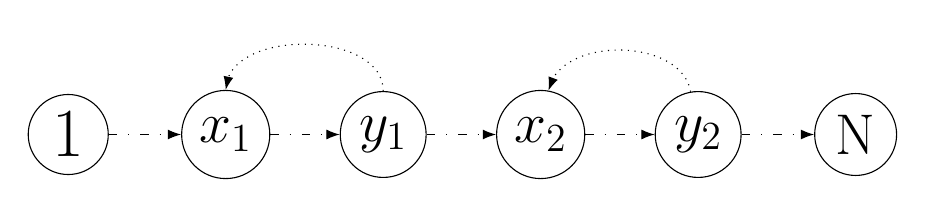
\begin{tikzpicture}
				\node[state] (root) {\Huge{$1$}};
				\node[state] (x1) [right of=root] {\huge{$x_1$}};
				\node[state] (y1) [right of=x1] {\huge{$y_1$}};
				\node[state] (x2) [right of=y1] {\huge{$x_2$}};
				\node[state] (y2) [right of=x2] {\huge{$y_2$}};
				\node[state] (N) [right of=y2] {\huge{N}};
				\path [dotteddirected] (root) edge (x1);
				\path [dotteddirected] (x1) edge (y1);
				\path [dotteddirected] (y1) edge (x2);
				\path [dotteddirected] (x2) edge (y2);
				\path [dotteddirected] (y2) edge (N);
				\path[reverseedge] (y1) edge[bend right=90] (x1);
				\path[reverseedge] (y2) edge[bend right=80] (x2);
		\end{tikzpicture}}
		\caption{Completely disjoint cycles}
		\label{Case1}
	\end{figure}
	\item \textbf{Case 2 (Edge-Disjoint Cycles Sharing a Node):} $x_1 < y_1 = x_2 < y_2$. The tail of reverse edge 1 coincides with the head of reverse edge 2 ($\mathcal{V}_1 \cap \mathcal{V}_2 = \{y_1\}$), as shown in Figure \ref{Case2}.
     \begin{figure}[ht!]
		\centering
		\scalebox{0.6}{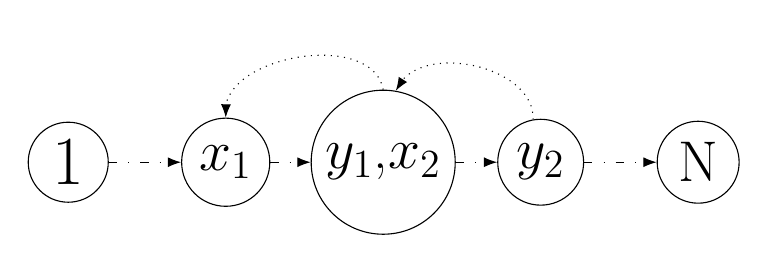
\begin{tikzpicture}
				\node[state] (root) {\Huge{$1$}};
				\node[state] (x1) [right of=root] {\huge{$x_1$}};
				\node[state] (y1) [right of=x1] {\huge{$y_1$,$x_2$}};
				\node[state] (y2) [right of=y1] {\huge{$y_2$}};
				\node[state] (N) [right of=y2] {\huge{N}};
				\path [dotteddirected] (root) edge (x1);
				\path [dotteddirected] (x1) edge (y1);
				\path [dotteddirected] (y1) edge (y2);
				\path [dotteddirected] (y2) edge (N);
				\path[reverseedge] (y1) edge[bend right=90] (x1);
				\path[reverseedge] (y2) edge[bend right=80] (y1);
		\end{tikzpicture}}
		\caption{Edge disjoint cycles sharing a common node}
		\label{Case2}
	\end{figure}
	\item \textbf{Case 3 (Partially Overlapping Cycles):} $x_1 < x_2 < y_1 < y_2$. The cycles share a common sub-chain of edges, but neither cycle is nested inside the other, as shown in Figure \ref{Case3}.
    \begin{figure}[ht!]
		\centering
		\scalebox{0.6}{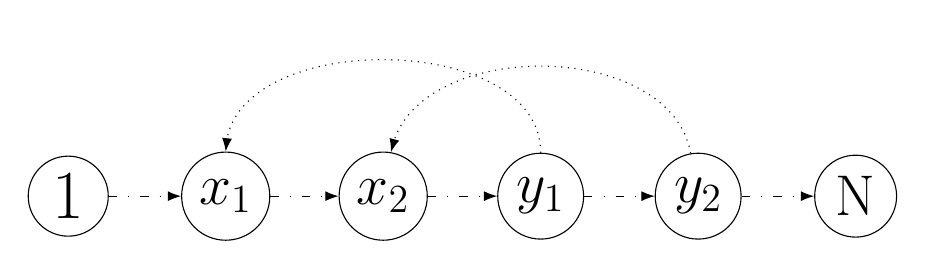
\begin{tikzpicture}
				\node[state] (root) {\Huge{$1$}};
				\node[state] (x1) [right of=root] {\huge{$x_1$}};
				\node[state] (x2) [right of=x1] {\huge{$x_2$}};
				\node[state] (y1) [right of=x2] {\huge{$y_1$}};
				\node[state] (y2) [right of=y1] {\huge{$y_2$}};
				\node[state] (N) [right of=y2] {\huge{N}};
				\path [dotteddirected] (root) edge (x1);
				\path [dotteddirected] (x1) edge (x2);
				\path [dotteddirected] (x2) edge (y1);
				\path [dotteddirected] (y1) edge (y2);
				\path [dotteddirected] (y2) edge (N);
				\path[reverseedge] (y1) edge[bend right=90] (x1);
				\path[reverseedge] (y2) edge[bend right=80] (x2);
		\end{tikzpicture}}
		\caption{Partially overlapping directed cycles}
        \label{Case3}
	\end{figure}
	\item \textbf{Case 4 (Fully Nested Cycles with Disjoint Reverse Edges):} $x_1 < x_2 < y_2 < y_1$. Cycle 2 is strictly contained within Cycle 1 ($\mathcal{V}_2 \subset \mathcal{V}_1$), and their reverse edges share no nodes, as shown in Figure \ref{Case4}.
    \begin{figure}[ht!]
		\centering
		\scalebox{0.6}{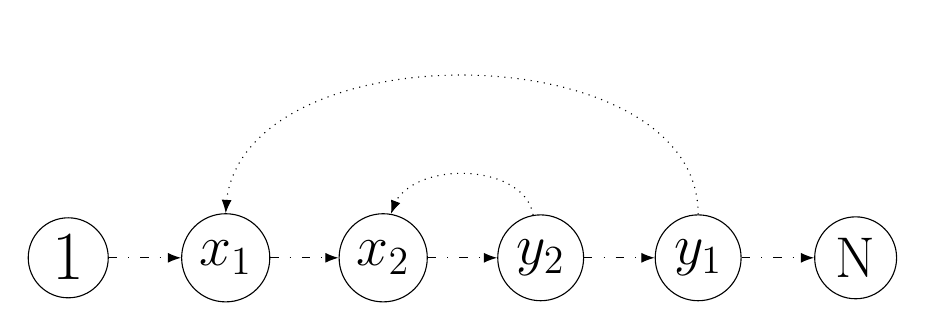
\begin{tikzpicture}
				\node[state] (root) {\Huge{$1$}};
				\node[state] (x1) [right of=root] {\huge{$x_1$}};
				\node[state] (x2) [right of=x1] {\huge{$x_2$}};
				\node[state] (y2) [right of=x2] {\huge{$y_2$}};
				\node[state] (y1) [right of=y2] {\huge{$y_1$}};
				\node[state] (N) [right of=y1] {\huge{N}};
				\path [dotteddirected] (root) edge (x1);
				\path [dotteddirected] (x1) edge (x2);
				\path [dotteddirected] (x2) edge (y2);
				\path [dotteddirected] (y2) edge (y1);
				\path [dotteddirected] (y1) edge (N);
				\path[reverseedge] (y1) edge[bend right=90] (x1);
				\path[reverseedge] (y2) edge[bend right=80] (x2);
		\end{tikzpicture}}
		\caption{Fully overlapping but reverse edges do not share nodes}
		\label{Case4}
	\end{figure} 
	\item \textbf{Case 5 (Fully Nested Cycles Sharing a Tail Node):} $x_1 < x_2 < y_1 = y_2$. Cycle 2 is contained in Cycle 1, and both reverse edges originate from the same tail node, as shown in Figure \ref{Case5}.
    \begin{figure}[ht!]
		\centering
		\scalebox{0.55}{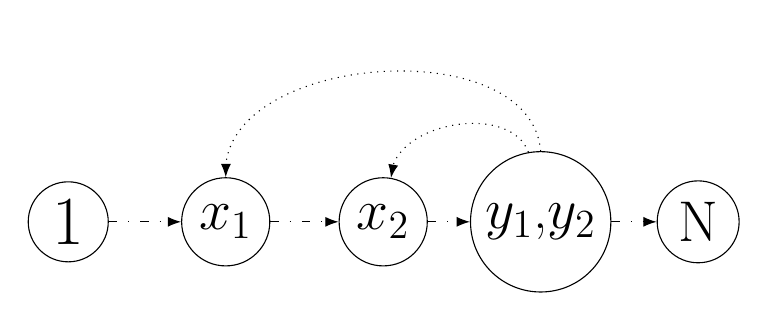
\begin{tikzpicture}
				\node[state] (root) {\Huge{$1$}};
				\node[state] (x1) [right of=root] {\huge{$x_1$}};
				\node[state] (x2) [right of=x1] {\huge{$x_2$}};
				\node[state] (y1) [right of=x2] {\huge{$y_1$,$y_2$}};
				\node[state] (N) [right of=y1] {\huge{N}};
				\path [dotteddirected] (root) edge (x1);
				\path [dotteddirected] (x1) edge (x2);
				\path [dotteddirected] (x2) edge (y1);
				\path [dotteddirected] (y1) edge (N);
				\path[reverseedge] (y1) edge[bend right=90] (x1);
				\path[reverseedge] (y1) edge[bend right=80] (x2);
		\end{tikzpicture}}
		\caption{Fully overlapping with shared tail node between the two reverse edges}
		\label{Case5}
	\end{figure}
	\item \textbf{Case 6 (Fully Nested Cycles Sharing a Head Node):} $x_1 = x_2 < y_2 < y_1$. Cycle 2 is contained in Cycle 1, and both reverse edges terminate at the same head node, as shown in Figure \ref{Case6}.
    \begin{figure}[ht!]
		\centering
		\scalebox{0.55}{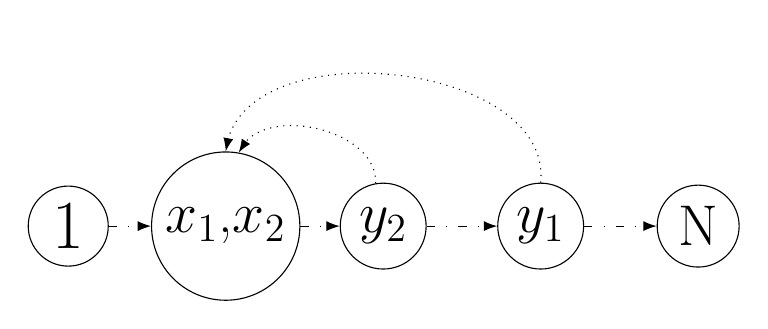
\begin{tikzpicture}
				\node[state] (root) {\Huge{$1$}};
				\node[state] (x1) [right of=root] {\huge{$x_1$,$x_2$}};
				\node[state] (y2) [right of=x1] {\huge{$y_2$}};
				\node[state] (y1) [right of=y2] {\huge{$y_1$}};
				\node[state] (N) [right of=y1] {\huge{N}};
				\path [dotteddirected] (root) edge (x1);
				\path [dotteddirected] (x1) edge (y2);
				\path [dotteddirected] (y2) edge (y1);
				\path [dotteddirected] (y1) edge (N);
				\path[reverseedge] (y1) edge[bend right=90] (x1);
				\path[reverseedge] (y2) edge[bend right=80] (x1);
		\end{tikzpicture}}
		\caption{Fully overlapping with shared head node between the two reverse edges}
		\label{Case6}
	\end{figure}
\end{enumerate}
Each of Cases 1–3 further splits into three length-based sub-cases: (a) $\ell_1 > \ell_2$, (b) $\ell_2 > \ell_1$, and (c) $\ell_1 = \ell_2$. Existing spectral analyses in \cite{zhang2017effect} address Case 1, while \cite{hao2019role} covers Cases 3(a), 4, and 5 under the restriction $|\ell_1 - \ell_2| \ge 1$. Consequently, Cases 2, 3(b), 3(c), and 6 remain completely unaddressed in the literature. In what follows, we present an exhaustive spectral analysis covering all six topological configurations without imposing any restrictive assumptions on the cycle lengths.

\subsection{Laplacian Determinant Expansions for Leader-Excluded Loops ($x_1 > 1$)}
When the root node remains external to both feedback loops ($x_1 > 1$), we have $d_{\text{in}, 1} = 0$, thereby preserving Node 1 as an autonomous leader. We now present exact determinant expansions and spectral proofs for all six topological configurations (Cases 1 through 6) alongside the general sufficiency theorem.

\begin{theo}[Spectral Boundary for Case 1 Topologies]\label{Theoremcase1}
Consider an $N$-node directed chain with unit forward edge weights containing two completely disjoint reverse edges under \textbf{Case 1} ($x_1 < y_1 < x_2 < y_2$). The dominant Laplacian convergence root $\lambda_2 = 1 - s_1$ is determined by the unique real solution $s_1 \in (0,1)$ of:
\begin{equation}\label{eq:case1_theorem_statement}
	\begin{cases}
		s^{\ell_1+1} + s^{\ell_1} - 1 = 0, & \text{if } \ell_1 > \ell_2 \\
		s^{\ell_2+1} + s^{\ell_2} - 1 = 0, & \text{if } \ell_2 > \ell_1 \\
		s^{\ell_1+1} + s^{\ell_1} - 1 = 0, & \text{if } \ell_1 = \ell_2
	\end{cases}
\end{equation}
\end{theo}

\begin{proof}
In Case 1, the two directed cycles share no common vertices ($\mathcal{V}_1 \cap \mathcal{V}_2 = \emptyset$). Under node ordering $1, 2, \dots, N$, the graph Laplacian $\mathcal{L} \in \mathbb{R}^{N \times N}$ is lower triangular everywhere except at two off-diagonal positions: $\mathcal{L}(x_1, y_1) = -1$ and $\mathcal{L}(x_2, y_2) = -1$. 
The characteristic matrix $(\lambda I_N - \mathcal{L})$ has the explicit structure:
\begin{equation}\label{eq:case1_matrix_structure}
	\lambda I_N - \mathcal{L} = \begin{bmatrix}
		\lambda & 0 & \dots & \dots & \dots & \dots & \dots & \dots & 0 & 0\\
		-1 & \lambda-1 & \dots & \dots & \dots & \dots & \dots & \dots & 0 & 0\\
		\vdots & \ddots & \ddots & \vdots & \vdots & \vdots & \vdots & \vdots & \vdots & \vdots \\
		0 & \dots & -1 & \lambda-2 & \dots & 1 & \dots & \dots & 0 & \vdots \\
		\vdots & \vdots & \vdots & \ddots & \ddots & \vdots & \vdots & \vdots & \vdots & \vdots \\
		0 & \dots & \dots & \dots & -1 & \lambda-1 & \dots & \dots & 0 & \vdots\\
		\vdots & \vdots & \vdots & \vdots & \vdots & \ddots & \ddots & \vdots & \vdots & \vdots \\
		0 & \dots & \dots & \dots & \dots & \dots & -1 & \lambda-2 & 1 & 0\\
		0 & \dots & \dots & \dots & \dots & \dots & \dots & 0 & -1 & \lambda-1
	\end{bmatrix}
\end{equation}
Expanding $|\lambda I_N - \mathcal{L}|$ via Laplace column expansions across unperturbed nodes yields:
\begin{equation}\label{eq:case1_det_decoupled}
	|\lambda I_N - \mathcal{L}| = \lambda (\lambda-1)^{N - (\ell_1 + \ell_2 + 2)} \cdot D_{\text{cycle1}}(\lambda) \cdot D_{\text{cycle2}}(\lambda)
\end{equation}
where $D_{\text{cycle1}}(\lambda)$ and $D_{\text{cycle2}}(\lambda)$ represent the characteristic determinants of the isolated single-loop subgraphs of lengths $\ell_1 = y_1 - x_1$ and $\ell_2 = y_2 - x_2$, respectively:
\begin{equation}
	D_{\text{cycle1}}(\lambda) = (\lambda-1)^{\ell_1+1} - (-1)^{\ell_1+1} = (\lambda-1)^{\ell_1+1} + (-1)^{\ell_1}
\end{equation}
\begin{equation}
	D_{\text{cycle2}}(\lambda) = (\lambda-1)^{\ell_2+1} - (-1)^{\ell_2+1} = (\lambda-1)^{\ell_2+1} + (-1)^{\ell_2}
\end{equation}

Substituting the spectral transformation $s = 1 - \lambda \implies \lambda - 1 = -s$ into $D_{\text{cycle1}}(s) \cdot D_{\text{cycle2}}(s) = 0$:
\begin{equation}
	\left[ (-s)^{l_1+1} + (-1)^{l_1} \right] \left[ (-s)^{l_2+1} + (-1)^{l_2} \right] = 0 \implies \left( s^{l_1+1} + s^{l_1} - 1 \right) \left( s^{l_2+1} + s^{l_2} - 1 \right) = 0
\end{equation}

Because the roots of the two disjoint subgraphs decouple completely, the maximum real root $s_1 \in (0,1)$ across the entire network is dictated exclusively by the longer cycle $\ell_i = \max(\ell_1, \ell_2)$, which produces the largest real root of $s^{\ell_i+1} + s^{\ell_i} = 1$. This completes the proof.
\end{proof}

\begin{theo}[Spectral Boundary for Case 2 Topologies]\label{Theoremcase2}
Consider an $N$-node directed chain with unit forward edge weights containing two reverse edges under \textbf{Case 2} ($y_1 = x_2$). The dominant Laplacian convergence root $\lambda_2 = 1 - s_1$ is determined by the unique real root $s_1 \in (0,1)$ of:
\begin{equation}\label{eq:case2_theorem_statement}
	\begin{cases}
		s^{\ell_1+1} + 2s^{\ell_1} + s^{\ell_1-1} - s^{\ell_1-\ell_2} - s^{\ell_1-\ell_2-1} = 1, & \text{if } \ell_1 > \ell_2 \\
		s^{\ell_2+2} + 2s^{\ell_2+1} + s^{\ell_2} - s^{\ell_2-\ell_1+1} - s = 1, & \text{if } \ell_2 > \ell_1 \\
		s^{\ell_2+2} + 2s^{\ell_2+1} + s^{\ell_2} - 2s = 1, & \text{if } \ell_1 = \ell_2
	\end{cases}
\end{equation}
\end{theo}

\begin{proof}
Let $\mathcal{L} \in \mathbb{R}^{N \times N}$ be the graph Laplacian matrix of the Case 2 chain network. Under node ordering $1, 2, \dots, N$, $\mathcal{L}$ is lower triangular everywhere except at two off-diagonal positions corresponding to the reverse edges: $\mathcal{L}(x_1, y_1) = -w_{r1} = -1$ and $\mathcal{L}(x_2, y_2) = -w_{r2} = -1$. 

The diagonal entries of $\mathcal{L}$ are $\ell_{ii} = d_{\text{in}, i} = 1$ for all nodes except the two head nodes $x_1$ and $x_2 = y_1$, which receive reverse edges and thus have $\ell_{x_1, x_1} = 2$ and $\ell_{x_2, x_2} = 2$.

The characteristic matrix $(\lambda I_N - \mathcal{L})$ has the explicit structure:
\begin{equation}
	\lambda I_N - \mathcal{L} = \begin{bmatrix}
		\lambda & 0 & \dots & \dots & \dots & \dots & 0 \\
		-1 & \lambda-1 & \dots & \dots & \dots & \dots & 0 \\
		\vdots & \ddots & \ddots & \vdots & \vdots & \vdots & \vdots \\
		0 & \dots & -1 & \lambda-2 & \dots & 1 & 0 \\
		\vdots & \vdots & \vdots & \ddots & \ddots & \vdots & \vdots \\
		0 & \dots & \dots & \dots & -1 & \lambda-2 & 1 \\
		0 & \dots & \dots & \dots & \dots & -1 & \lambda-1
	\end{bmatrix}
\end{equation}

Expanding the determinant $|\lambda I_N - \mathcal{L}|$ using Laplace column expansions across the decoupled unperturbed blocks $\{1, \dots, x_1-1\}$ and $\{y_2+1, \dots, N\}$ yields:
\begin{equation}\label{eq:det_decoupled}
	|\lambda I_N - \mathcal{L}| = \lambda (\lambda-1)^{x_1-2} (\lambda-1)^{N-y_2} \cdot D_{\text{core}}(\lambda)
\end{equation}
where $D_{\text{core}}(\lambda)$ is the determinant of the sub-block spanning nodes $x_1$ through $y_2$. 

Applying Laplace minor expansions across the two feedback cycles of lengths $\ell_1 = y_1 - x_1$ and $\ell_2 = y_2 - x_2$ (with $y_1 = x_2$):
\begin{equation}\label{eq:D_core_expansion}
	D_{\text{core}}(\lambda) = (\lambda-2) \left\{ (\lambda-1)^{\ell_1-1} \left[ (\lambda-2)(\lambda-1)^{\ell_2} + (-1)^{\ell_2} \right] \right\} + (-1)^{\ell_1} (\lambda-1)^{\ell_2}
\end{equation}
Distributing the terms inside $D_{\text{core}}(\lambda)$:
\begin{equation}\label{eq:D_core_expanded}
	D_{\text{core}}(\lambda) = (\lambda-2)^2 (\lambda-1)^{\ell_1+\ell_2-1} + (-1)^{\ell_2}(\lambda-2)(\lambda-1)^{\ell_1-1} + (-1)^{\ell_1}(\lambda-1)^{\ell_2}
\end{equation}

We now substitute the spectral transformation $s = 1 - \lambda \implies \lambda - 1 = -s$ and $\lambda - 2 = -(s+1)$ into \eqref{eq:D_core_expanded}:
\begin{align}
	D_{\text{core}}(s) &= [-(s+1)]^2 (-s)^{\ell_1+\ell_2-1} + (-1)^{\ell_2}[-(s+1)](-s)^{\ell_1-1} + (-1)^{\ell_1}(-s)^{\ell_2} \nonumber \\
	&= (s+1)^2 (-1)^{\ell_1+\ell_2-1} s^{\ell_1+\ell_2-1} + (-1)^{\ell_2} (-1)^{\ell_1} (s+1) s^{\ell_1-1} + (-1)^{\ell_1} (-1)^{\ell_2} s^{\ell_2} \nonumber \\
	&= (-1)^{\ell_1+\ell_2} \left[ -(s+1)^2 s^{\ell_1+\ell_2-1} + (s+1) s^{\ell_1-1} + s^{\ell_2} \right]
\end{align}

Setting $D_{\text{core}}(s) = 0$ yields the fundamental characteristic relation:
\begin{equation}\label{eq:core_s_relation}
	(s+1)^2 s^{\ell_1+\ell_2-1} - (s+1) s^{\ell_1-1} - s^{\ell_2} = 0
\end{equation}

We now analyze the three sub-cases based on the relative cycle lengths $\ell_1$ and $\ell_2$:

\vspace{0.5em}
\textbf{Sub-case 2(a): $\ell_1 > \ell_2$}\\
Divide equation \eqref{eq:core_s_relation} by $s^{\ell_2} > 0$ for $s \in (0,1)$:
\begin{equation}
	(s+1)^2 s^{\ell_1-1} - (s+1) s^{\ell_1-\ell_2-1} - 1 = 0
\end{equation}
Expanding $(s+1)^2 s^{\ell_1-1} = (s^2 + 2s + 1) s^{\ell_1-1} = s^{\ell_1+1} + 2s^{\ell_1} + s^{\ell_1-1}$, and expanding $(s+1) s^{\ell_1-l_2-1} = s^{\ell_1-\ell_2} + s^{\ell_1-\ell_2-1}$:
\begin{equation}
	s^{\ell_1+1} + 2s^{\ell_1} + s^{\ell_1-1} - s^{\ell_1-\ell_2} - s^{\ell_1-\ell_2-1} = 1
\end{equation}
which matches the first line of \eqref{eq:case2_theorem_statement}.

\vspace{0.5em}
\textbf{Sub-case 2(b): $\ell_2 > \ell_1$}\\
Divide equation \eqref{eq:core_s_relation} by $s^{\ell_1-1} > 0$ for $s \in (0,1)$:
\begin{equation}
	(s+1)^2 s^{\ell_2} - (s+1) - s^{\ell_2-\ell_1+1} = 0
\end{equation}
Expanding $(s+1)^2 s^{\ell_2} = s^{\ell_2+2} + 2s^{\ell_2+1} + s^{\ell_2}$:
\begin{equation}
	s^{\ell_2+2} + 2s^{\ell_2+1} + s^{\ell_2} - s^{\ell_2-\ell_1+1} - s = 1
\end{equation}
which matches Lemma \ref{Lemma:ch_TRE_poly2} and the second line of \eqref{eq:case2_theorem_statement}.

\vspace{0.5em}
\textbf{Sub-case 2(c): $l_1 = l_2$}\\
Substitute $l_1 = l_2$ into equation \eqref{eq:core_s_relation}:
\begin{equation}
	(s+1)^2 s^{\ell_2} - (s+1) - s = 0 \implies s^{\ell_2+2} + 2s^{\ell_2+1} + s^{\ell_2} - 2s = 1
\end{equation}
which matches Lemma \ref{Lemma:ch_TRE_poly1} and the third line of \eqref{eq:case2_theorem_statement}.
\end{proof}

\begin{theo}[Spectral Boundary for Case 3 Topologies]\label{theo9}
Consider an $N$-node directed chain under \textbf{Case 3} (partially overlapping cycles, $x_1 < x_2 < y_1 < y_2$). The dominant Laplacian convergence root $\lambda_2 = 1 - s_1$ is determined by the unique real solution $s_1 \in (0,1)$ of:
\begin{equation}
	\begin{cases}
		s^{\ell_1+1} + 2s^{\ell_1} + s^{\ell_1-1} - s^{\ell_1-\ell_2} - s^{\ell_1-\ell_2-1} = 1, & \text{if } \ell_1 > \ell_2 \\
		s^{\ell_2+2} + 2s^{\ell_2+1} + s^{\ell_2} - s^{\ell_2-\ell_1+1} - s = 1, & \text{if } \ell_2 > \ell_1 \\
		s^{\ell_2+2} + 2s^{\ell_2+1} + s^{\ell_2} - 2s = 1, & \text{if } \ell_1 = \ell_2
	\end{cases}
\end{equation}
\end{theo}

\begin{proof}
In Case 3, the reverse edges overlap over the node subset $\{x_2, \dots, y_1\}$. Writing the core Laplacian determinant across the overlapping sub-blocks and performing successive row reductions yields a reduced characteristic determinant identical to $D_{\text{core}}(s)$ in \eqref{eq:D_core_expanded}. Dividing by common powers of $s$ across sub-cases $\ell_1 > \ell_2$, $\ell_2 > \ell_1$, and $\ell_1 = \ell_2$ produces the identical polynomial equations as in Case 2.
\end{proof}

\begin{theo}[Spectral Boundary for Case 4 Topologies]\label{Theoremcase4}
Consider an $N$-node directed chain with unit forward edge weights containing two fully nested reverse edges under \textbf{Case 4} ($x_1 < x_2 < y_2 < y_1$, with $\ell_1 > \ell_2$). The dominant Laplacian convergence root $\lambda_2 = 1 - s_1$ is determined by the unique real solution $s_1 \in (0,1)$ of
\begin{equation}\label{eq:case4_theorem_statement}
	s^{\ell_1+1} + 2s^{\ell_1} + s^{\ell_1-1} - s^{\ell_1-\ell_2} - s^{\ell_1-\ell_2-1} = 1.
\end{equation}
\end{theo}

\begin{proof}
In Case 4, Cycle 2 ($y_2 - x_2 = \ell_2$) is fully nested inside Cycle 1 ($y_1 - x_1 = \ell_1$), with $x_1 < x_2$ and $y_2 < y_1$. The head nodes $x_1$ and $x_2$ each receive one reverse edge, giving in-degrees $l_{x_1, x_1} = 2$ and $l_{x_2, x_2} = 2$. 

Expanding the determinant $|\lambda I_N - \mathcal{L}|$, to obtain the characteristic polynomial, along the nested feedback blocks yields:
\begin{equation}\label{eq:case4_det_expansion}
	D_{\text{core}}(\lambda) = (\lambda-2)^2 (\lambda-1)^{\ell_1+\ell_2-1} + (-1)^{\ell_2}(\lambda-2)(\lambda-1)^{\ell_1-1} + (-1)^{\ell_1}(\lambda-1)^{\ell_2}
\end{equation}
Substituting the spectral transformation $s = 1 - \lambda \implies \lambda - 1 = -s$ and $\lambda - 2 = -(s+1)$ into \eqref{eq:case4_det_expansion} and dividing by $s^{\ell_2}$ (since $\ell_1 > \ell_2$ holds strictly for nested configurations) produces:
\begin{equation}
	s^{\ell_1+1} + 2s^{\ell_1} + s^{\ell_1-1} - s^{\ell_1-\ell_2} - s^{\ell_1-\ell_2-1} = 1
\end{equation}
which establishes the equivalence between Case 4 and the $\ell_1 > \ell_2$ sub-case of Case 2.
\end{proof}

\begin{theo}[Spectral Boundary for Case 5 Topologies]\label{Theoremcase5}
Consider an $N$-node directed chain under \textbf{Case 5} (nested cycles sharing tail node $y_1 = y_2$, with $\ell_1 > \ell_2$). The dominant Laplacian convergence root $\lambda_2 = 1 - s_1$ is determined by the unique real solution $s_1 \in (0,1)$ of:
\begin{equation}\label{eq:case5_theorem_statement}
	s^{\ell_1+1} + 2s^{\ell_1} + s^{\ell_1-1} - s^{\ell_1-\ell_2} - s^{\ell_1-\ell_2-1} = 1
\end{equation}
\end{theo}

\begin{proof}
In Case 5, both reverse edges originate from the shared tail node $y_1 = y_2$ and terminate at distinct head nodes $x_1$ and $x_2$ ($x_1 < x_2$). Nodes $x_1$ and $x_2$ have in-degrees $d_{\text{in}, x_1} = 2$ and $d_{\text{in}, x_2} = 2$. 

Expanding $|\lambda I_N - \mathcal{L}|$ along row $y_1$ and substituting $s = 1 - \lambda$ yields the characteristic equation $(s+1)^2 s^{\ell_1-1} - (s+1) s^{\ell_1-\ell_2-1} - 1 = 0$. Expanding this relation directly gives $s^{\ell_1+1} + 2s^{\ell_1} + s^{\ell_1-1} - s^{\ell_1-\ell_2} - s^{\ell_1-\ell_2-1} = 1$, completing the proof.
\end{proof}

\begin{theo}[Spectral Boundary for Case 6 Topologies]\label{theo10}
Consider an $N$-node directed chain under \textbf{Case 6} (nested cycles sharing head node $x_1 = x_2$, with $\ell_1 > \ell_2$). The dominant Laplacian convergence root $\lambda_2 = 1 - s_1$ is determined by the unique real solution $s_1 \in (0,1)$ of:
\begin{equation}\label{eq:case6_statement}
	s^{\ell_1}(s+2) - s^{\ell_1-\ell_2} = 1
\end{equation}
\end{theo}

\begin{proof}
When $x_1 = x_2$, Node $x_1$ receives two incoming reverse edges (from $y_1$ and $y_2$). Thus, its in-degree is $d_{\text{in}, x_1} = 3$, giving diagonal entry $l_{x_1, x_1} = 3$. Expanding $|\lambda I_N - \mathcal{L}|$ along row $x_1$:
\begin{equation}
	|\lambda I - \mathcal{L}| = \lambda (\lambda-1)^{N-\ell_1-1} \left[ (\lambda-1)^{\ell_1}(\lambda-2) + (\lambda-1)^{\ell_1-\ell_2} - 1 \right] = 0
\end{equation}
Substituting $s = 1 - \lambda \implies \lambda - 1 = -s$ and $\lambda - 2 = -(s+1)$:
\begin{equation}
	(-s)^{\ell_1}[-(s+1)] + (-s)^{\ell_1-\ell_2} - 1 = 0 \implies s^{\ell_1}(s+2) - s^{\ell_1-\ell_2} = 1
\end{equation}
which matches Lemma \ref{Lemma:ch_TRE_poly3} and completes the proof.
\end{proof}









\begin{theo}[Velocity Coupling Threshold for Dual-Loop Topologies]\label{theo11}
\leavevmode\par\noindent
Asymptotic second-order consensus, $\lim_{t \to \infty} \|p_i(t) - p_j(t)\| = 0$ and $\lim_{t \to \infty} \|v_i(t) - v_j(t)\| = 0$, is guaranteed for an $N$-agent directed chain with two reverse edges under Cases 1–6 (with $x_1 > 1$) if the velocity coupling parameter $\gamma$ satisfies:
\begin{equation}\label{new-sufficiency}
	\gamma \ge \frac{1}{\sqrt{1 - s_1}}
\end{equation}
where $s_1 \in (0,1)$ is the unique real solution of the corresponding characteristic polynomial equation (\eqref{eq:ch_TRE_Poly1}, \eqref{eq:ch_TRE_Poly2}, or \eqref{eq:ch_TRE_poly3}).
\end{theo}

\begin{proof}
Recall from Lemma \ref{eq:ren_gamma_bound} (Ren \cite{ren2008consensus}) that second-order consensus is guaranteed if:
\begin{equation}\label{eq:ch_TRE_ren_suff_proof}
	\gamma \ge \max_{i \in \{2, \dots, N\}} \sqrt{\frac{2}{\mathfrak{Re}(\lambda_i)}}
\end{equation}
While condition \eqref{eq:ch_TRE_ren_suff_proof} is sufficient, Yu et al. \cite{yu2010some} established that consensus is preserved whenever $\gamma \ge \max_i \sqrt{1/\mathfrak{Re}(\lambda_i)}$ as stated in \eqref{eq:ch_TRE_yuexactbound}. 

By Lemmas \ref{Lemma:ch_TRE_poly1}–\ref{Lemma:ch_TRE_poly3}, the unique real root $s_1 \in (0,1)$ of the transformed polynomial dominates the real parts of all other roots ($c = \mathfrak{Re}(r) < s_1$). Under the mapping $\lambda_i = 1 - r_i$, this establishes that $\lambda_2 = 1 - s_1$ is strictly the minimum real part across the non-zero Laplacian spectrum:
\begin{equation}
	\mathfrak{Re}(\lambda_i) \ge \mathfrak{Re}(\lambda_2) = 1 - s_1 > 0, \quad \forall i \in \{2, \dots, N\}
\end{equation}
Substituting $\mathfrak{Re}(\lambda_2) = 1 - s_1$ into the critical threshold yields:
\begin{equation}\label{eq:ch_TRE_DubeyBound}
	\gamma \ge \frac{1}{\sqrt{\mathfrak{Re}(\lambda_2)}} = \frac{1}{\sqrt{1 - s_1}}
\end{equation}
which guarantees that the sufficient stability criterion is satisfied.
\end{proof}

\subsection{The Root-Node Loop Structural Singularity}

We now investigate the critical structural transition that occurs when a reverse feedback edge enters Node 1 (the root) itself ($x_1 = 1$).

\begin{theo}[Eigenvalue Shift Theorem for Root-Node Loops]\label{theo12}
\leavevmode\par\noindent
Consider an $N$-node directed chain containing a reverse edge that forms a directed cycle of length $\ell$. The addition of this reverse edge alters exactly $\ell+1$ eigenvalues of the graph Laplacian $\mathcal{L}$ if the root node is excluded ($x_1 > 1$), but alters exactly $\ell$ non-zero eigenvalues if the root node participates in loop formation ($x_1 = 1$).
\end{theo}
\begin{proof}
\textbf{Case 1: Root Node Excluded ($x_1 > 1$)}\\
When $x_1 > 1$, Node 1 retains $d_{\text{in}, 1} = 0$. The nominal chain Laplacian $\mathcal{L}$ can be block-partitioned as:
\begin{equation}
	\mathcal{L} = \begin{bmatrix}
		\mathcal{L}_1 & 0 & 0 \\
		* & \Phi & 0 \\
		* & * & \mathcal{L}_2
	\end{bmatrix}
\end{equation}
where $\mathcal{L}_1 \in \mathbb{R}^{(x_1-1) \times (x_1-1)}$ represents the unperturbed leader sub-chain, $\Phi \in \mathbb{R}^{(\ell+1) \times (\ell+1)}$ represents the cycle sub-chain, and $\mathcal{L}_2 \in \mathbb{R}^{(N-y_1) \times (N-y_1)}$ represents the downstream sub-chain. 

Adding the reverse edge inserts a perturbation matrix $P$:
\begin{equation}
	P = \begin{bmatrix}
		0 & 0 & 0 \\
		0 & \Delta & 0 \\
		0 & 0 & 0
	\end{bmatrix}
\end{equation}
where $\Delta \in \mathbb{R}^{(\ell+1) \times (\ell+1)}$ contains non-zero entries only at the feedback positions. The perturbed Laplacian is $\mathcal{L}_c = \mathcal{L} + P$. Computing the characteristic polynomials:
\begin{equation}
	|\lambda I - \mathcal{L}| = |\lambda I - \mathcal{L}_1| \cdot |\lambda I - \Phi| \cdot |\lambda I - \mathcal{L}_2| = 0
\end{equation}
\begin{equation}
	|\lambda I - \mathcal{L}_c| = |\lambda I - \mathcal{L}_1| \cdot |\lambda I - (\Phi + \Delta)| \cdot |\lambda I - \mathcal{L}_2| = 0
\end{equation}
Comparing the spectrum of $\mathcal{L}$ and $\mathcal{L}_c$, only the eigenvalues corresponding to $|\lambda I - \Phi| = 0$ are modified to roots of $|\lambda I - (\Phi + \Delta)| = 0$. Since $\Phi \in \mathbb{R}^{(\ell+1) \times (\ell+1)}$, exactly $\text{dim}(\Phi) = \ell+1$ eigenvalues are shifted.

\vspace{0.5em}
\textbf{Case 2: Root Node Included ($x_1 = 1$)}\\
When $x_1 = 1$, the reverse edge terminates at Node 1. The sub-block $\mathcal{L}_1$ disappears, and $\mathcal{L}$ and $P$ partition as:
\begin{equation}
	\mathcal{L} = \begin{bmatrix}
		\Phi & 0 \\
		* & \mathcal{L}_2
	\end{bmatrix}, \quad
	P = \begin{bmatrix}
		\Delta & 0 \\
		0 & 0
	\end{bmatrix} \implies
	\mathcal{L}_c = \begin{bmatrix}
		\Phi + \Delta & 0 \\
		* & \mathcal{L}_2
	\end{bmatrix}
\end{equation}
where $\Phi, \Delta \in \mathbb{R}^{(\ell+1) \times (\ell+1)}$. 

The characteristic polynomials are $|\lambda I - \mathcal{L}| = |\lambda I - \Phi| \cdot |\lambda I - \mathcal{L}_2| = 0$ and $|\lambda I - \mathcal{L}_c| = |\lambda I - (\Phi + \Delta)| \cdot |\lambda I - \mathcal{L}_2| = 0$. 

By definition of graph Laplacians, every row sum of $\mathcal{L}_c$ is identically zero ($\mathcal{L}_c \mathbf{1}_N = 0_{N, 1}$), guaranteeing that $\lambda_1 = 0$ is always an eigenvalue. Since $\mathcal{L}_2$ is strictly lower triangular with unit diagonal entries ($\ell_{ii} = 1$), $\det(\mathcal{L}_2) = 1 \neq 0$, meaning $\mathcal{L}_2$ has no zero eigenvalues. Consequently, the zero eigenvalue $\lambda_1 = 0$ resides strictly within the sub-block $(\Phi + \Delta)$ and is structurally invariant ($0 \in \sigma(\Phi)$ and $0 \in \sigma(\Phi + \Delta)$). 

Thus, out of the $\ell+1$ total dimensions of $(\Phi + \Delta)$, one eigenvalue is permanently fixed at zero, meaning that adding a root-node loop alters at most $(\ell+1) - 1 = \ell$ non-zero eigenvalues.
\end{proof}

\subsection{Collapse of Polynomial Spectral Analysis method under Loops involving Root-Node}
When $x_1 = 1$, substituting $x_1 = 1$ into the general characteristic determinants for Cases 1–6 yields the following reduced polynomial relations in terms of $s = 1 - \lambda$:
\begin{enumerate}
	\item \textbf{Case 1 ($x_1 = 1$):} $s^{l_1+1} = 1 \implies s_1 = 1$.
	\item \textbf{Cases 2, 3, 4, 5 ($x_1 = 1$):} $s^{l_i+1} + s^{l_i} - s^{|l_1-l_2|} = 1 \implies s_1 = 1$, where $l_i = \max(l_1, l_2)$.
	\item \textbf{Cases 2, 3 ($x_1 = 1, l_1 = l_2$):} $s^{l_1+1} + s^{l_1} = 2 \implies s_1 = 1$.
	\item \textbf{Case 6 ($x_1 = 1$):} $s^{l_1+1} + s^{l_1} - s^{l_1-l_2} = 1 \implies s_1 = 1$.
\end{enumerate}

In each of the above scenarios, evaluating the transformed polynomial at $s = 1$ yields $p(1) = 1$. Consequently, $s_1 = 1$ is an exact root of all reduced polynomials when the root node participates in a feedback loop. 

Under the inverse transformation $\lambda = 1 - s$, $s_1 = 1$ maps to:
\begin{equation}
	\lambda_2 = 1 - s_1 = 1 - 1 = 0
\end{equation}

This reveals a fundamental theoretical limitation-- when the leader/root node is embedded inside a feedback loop, standard characteristic polynomial methods yield the trivial bound $\lambda_2 \ge 0$. Because $d_{\text{in}, 1} > 0$, Node 1 loses its autonomous authority, degenerating the leader-follower hierarchy and transforming every node within the cycle into an equivalent root node. 

Since $\lambda_2 = 0$ provides no actionable information regarding the critical velocity coupling threshold $\gamma$, characteristic polynomial methods are inherently incapable of providing sufficient conditions for second-order consensus when cycles involve the root-node. This structural singularity establishes the direct mathematical motivation for Chapter \ref{ch:Guaranteed_Consensus}, where localized edge/node scaling algorithms and a retuning based on the root-locus technique are formulated to resolve the breakdown of consensus when the cycle involves the root node.

\section{Simulations} 
\subsection{Second-order consensus in network with directed topology as in Case~\ref{Case2}}
Consider the network topology shown in Fig.~\ref{Case2}, with $N=30$, $x_1=12$, $y_1=x_2=16$, and $y_2=26$. Applying Theorems~\ref{Theoremcase2} and~\ref{theo11}, the real root obtained for the considered topology is $s=0.0333$. Accordingly, the sufficient velocity coupling parameter for achieving second-order consensus is calculated as
\begin{equation}
    \gamma_{\mathrm{suff}}
    =\frac{1}{\sqrt{s}}
    =\frac{1}{\sqrt{0.0333}}
    \approx 5.4763.
\end{equation}
Figure~\ref{Case2bconsensus} shows the position and velocity trajectories of all agents for $\gamma=\gamma_{\mathrm{suff}}=5.4763$. Both position and velocity consensus are achieved, with the corresponding trajectories illustrating their transient convergence behaviour.

Since the condition provided by Theorems~\ref{Theoremcase2} and~\ref{theo11} is sufficient but not necessary, consensus may also be achieved for values of $\gamma$ below the calculated sufficient bound. To investigate this possibility, an additional simulation is performed with the coupling parameter selected as $95\%$ of the sufficient value:
\begin{equation}
    \gamma_1=0.95\gamma_{\mathrm{suff}}
    =0.95\times5.4763
    \approx 5.2025.
\end{equation}
As shown in Fig.~\ref{Case2bconsensus_below_calculated_gamma}, both position and velocity consensus are still achieved. This confirms that the sufficient coupling bound is conservative and that consensus can be attained for a smaller value of $\gamma$.

For further comparison, the exact stability threshold is evaluated using the necessary and sufficient condition for second-order consensus:
\begin{equation}
    \gamma_{\mathrm{stab}}
    =
    \max_{i\in\{2,\ldots,N\}}
    \left[
    \frac{|\mathfrak{Im}(\lambda_i)|}{|\lambda_i|}
    \sqrt{\frac{1}{\mathfrak{Re}(\lambda_i)}}
    \right]
    =1.7532.
\end{equation}
To examine the system response below this threshold, another simulation is performed with
\begin{equation}
    \gamma_2=0.95\gamma_{\mathrm{stab}}
    =0.95\times1.7532
    \approx 1.6655.
\end{equation}
The resulting position and velocity trajectories, shown in Fig.~\ref{Case2bconsensus_Below_Threshold}, demonstrate the breakdown of consensus.

The three simulations collectively illustrate the distinction between the sufficient coupling bound and the exact stability threshold. In particular, consensus is achieved for $\gamma=5.2025$, even though this value is below the sufficient bound of $5.4763$. However, reducing the coupling parameter below the exact stability threshold of $1.7532$ results in consensus failure. Thus, the sufficient condition provides a conservative guarantee, whereas the necessary and sufficient condition identifies the actual stability boundary for the considered network.

\begin{figure}[ht!]
\centering
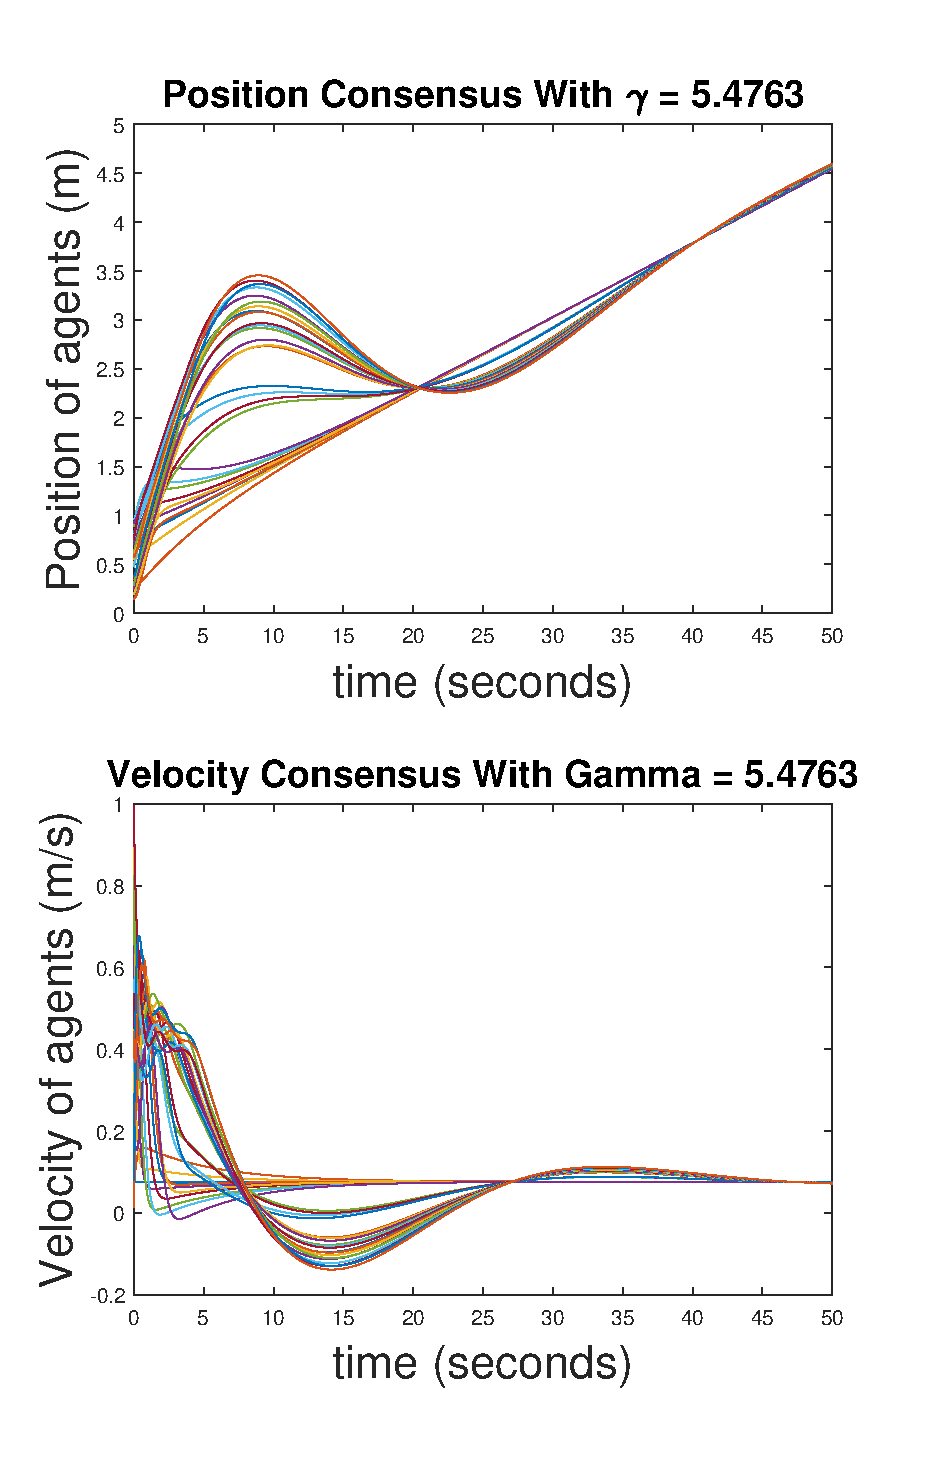
\includegraphics[width=0.75\textwidth,keepaspectratio]{2_Images/2.4.1_Position_Velocity_Combined_Sufficient_Gamma.eps}
\caption{Position and velocity consensus in the presence of two reverse edges, where $x_1<x_2=y_1<y_2$.}
\label{Case2bconsensus}
\end{figure}

\begin{figure}[ht!]
\centering
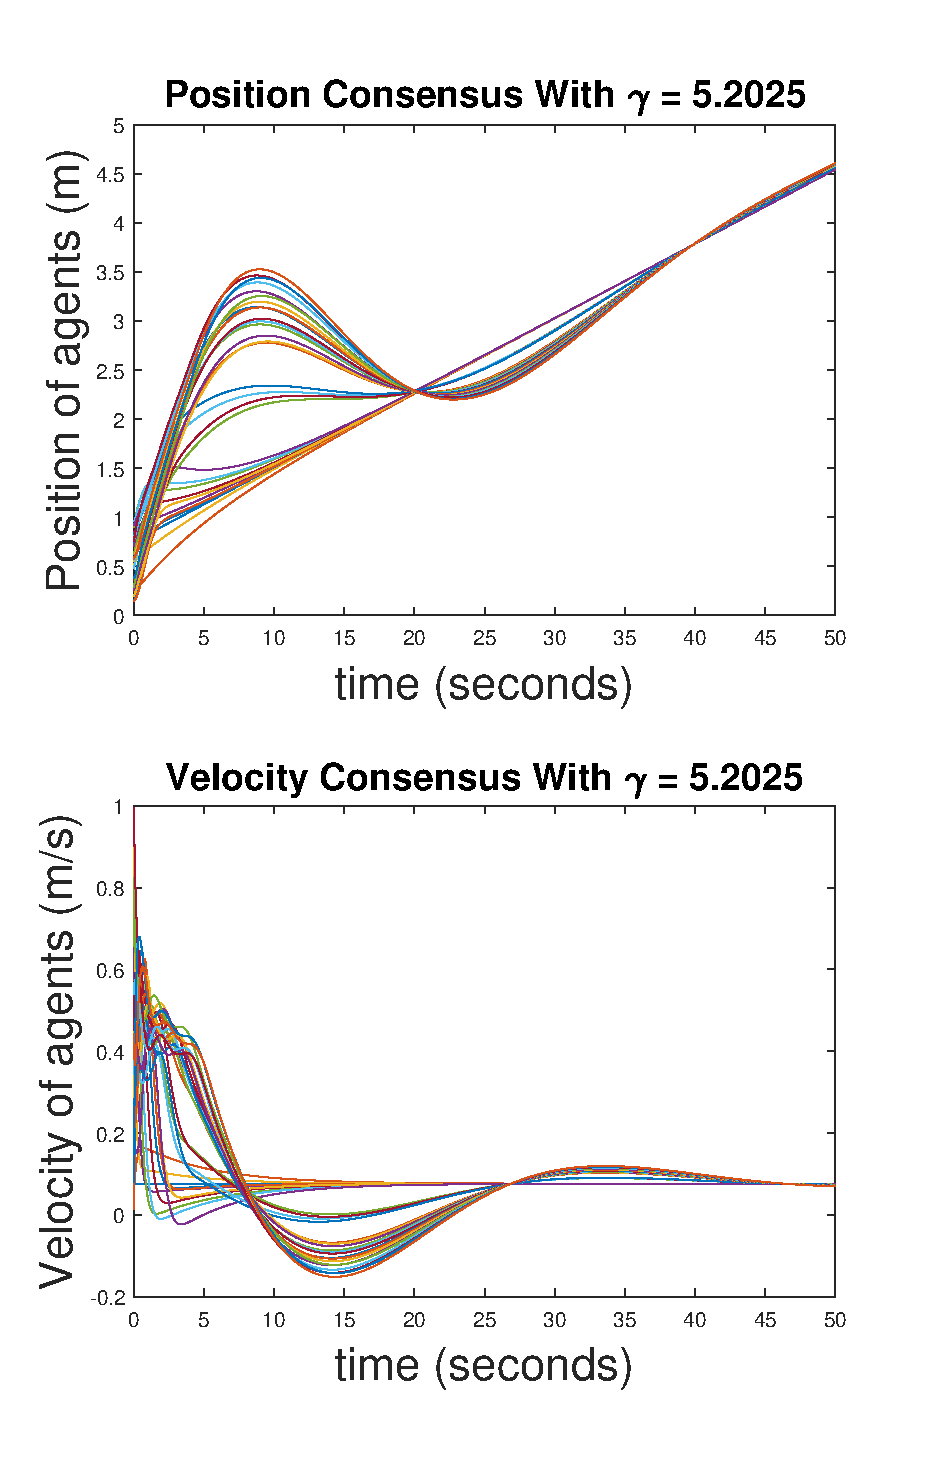
\includegraphics[width=0.75\textwidth,keepaspectratio]{2_Images/2.4.1_Position_Velocity_Combined_Below_Sufficient_Gamma.eps}
\caption{Position and velocity responses for a velocity coupling parameter slightly below the calculated sufficient value.}
\label{Case2bconsensus_below_calculated_gamma}
\end{figure}

\begin{figure}[ht!]
\centering
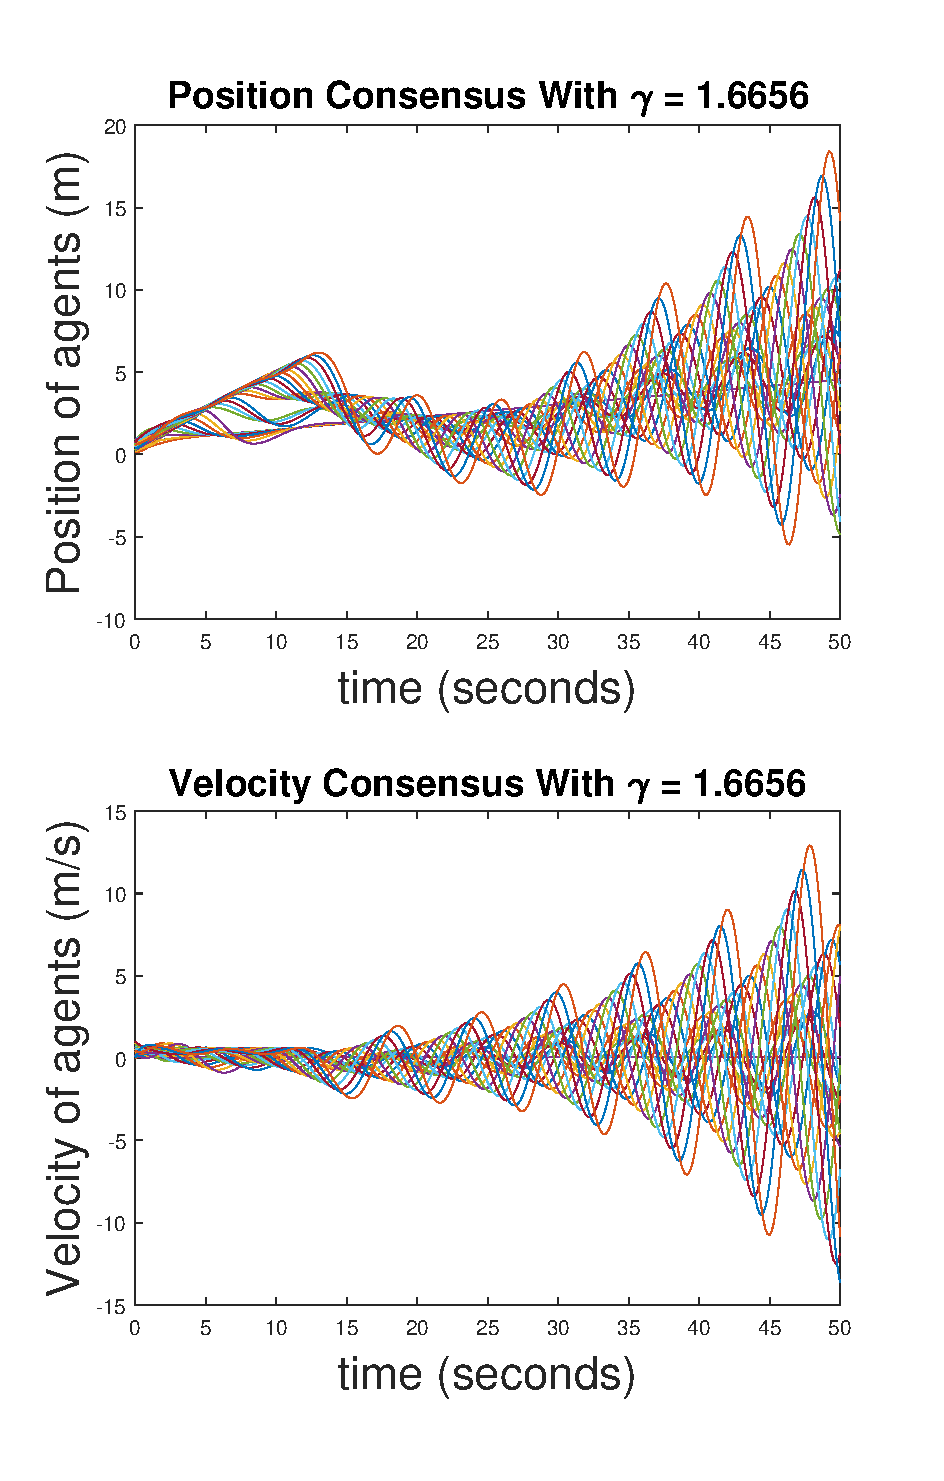
\includegraphics[width=0.75\textwidth,keepaspectratio]{2_Images/2.4.1_Position_Velocity_Combined_Below_Threshold_Gamma.eps}
\caption{Breakdown of position and velocity consensus when the velocity coupling parameter is below the stability threshold.}
\label{Case2bconsensus_Below_Threshold}
\end{figure}

\subsection{Second-order consensus in directed topology of Case~\ref{Case3}(c)}
%	Consider the network as shown in Fig.~\ref{Case3}, with $N=30$, $x_1=10$, $x_2=15$, $y_1=20$ and $y_2=25$. Applying Theorems \ref{theo9} and \ref{theo11}, for consensus of double integrators, the real solution obtained is equal to 0.0275 and corresponding $\gamma=6.0339$. As we can see from Figure~\ref{Case3cconsensus}, the consensus in position is achieved with the given $\gamma$ value. Positional consensus establishes the fact that consensus in velocity has also been achieved, since otherwise positional consensus would have been untenable. Hence, positional consensus is sufficient to conclude about consensus in all the states of the multi-agent system in this case. However, for completeness, the velocity consensus plot has also been included in the figure.

% The gamma value calculated above is as per sufficiency condition. However, if the gamma is calculated as per necessary and sufficient condition given in \ref{eq:ch_TRE_yuexactbound}, the value of $\gamma=2.3216$. To show the consensus breakdown, a simulation with $\gamma=0.95*2.3216=2.2055$ is shown in Fig \ref{Case3cconsensusBreakdown}.

To validate the theoretical bounds established in Theorem~\ref{theo9} and Theorem~\ref{theo11}, we consider the directed chain network depicted in Fig.~\ref{Case3} with $N = 30$ second-order agents. The reverse feedback edges are configured with coordinates $x_1 = 10$, $x_2 = 15$, $y_1 = 20$, and $y_2 = 25$. 

This network realization corresponds to Case~3(c) (partially overlapping feedback loops of equal cycle length), where:
\begin{equation}
    l_1 = y_1 - x_1 = 10, \quad l_2 = y_2 - x_2 = 10.
\end{equation}
Substituting $l_1 = l_2 = 10$ into the characteristic polynomial defined in Theorem~\ref{theo9} yields:
\begin{equation}
    s^{12} + 2s^{11} + s^{10} - 2s = 1.
    \label{eq:sim_char_poly}
\end{equation}
By Lemma~\ref{Lemma:ch_TRE_poly1}, \eqref{eq:sim_char_poly} possesses a unique real root in $(0, 1)$, numerically evaluated as $s_1 = 0.0275$. The corresponding dominant convergence rate is $\mathfrak{Re}(\lambda_2(\mathcal{L})) = 1 - s_1 = 0.9725$. Applying the sufficiency condition formulated in Theorem~\ref{theo11}, the required velocity coupling gain evaluates to:
\begin{equation}
    \gamma_{\text{suff}} = \frac{1}{\sqrt{1 - s_1}} = \frac{1}{\sqrt{0.9725}} \approx 6.0339.
\end{equation}

As demonstrated in Fig.~\ref{Case3cconsensus}, choosing $\gamma = 6.0339$ guarantees asymptotic agreement among the agent states. Positional consensus $\lim_{t \to \infty} \|p_i(t) - p_j(t)\| = 0$ inherently guarantees velocity synchronization $\lim_{t \to \infty} \|v_i(t) - v_j(t)\| = 0$, as double-integrator dynamics ($\dot{p}_i = v_i$) render persistent positional alignment untenable in the presence of velocity divergence. Consequently, achieving positional consensus is mathematically sufficient to certify full-state consensus; nevertheless, the velocity profile is provided in Fig.~\ref{Case3cconsensus} for completeness.

While the value $\gamma = 6.0339$ satisfies the sufficiency condition of Theorem~\ref{theo11}, the exact stability boundary is dictated by the necessary and sufficient condition given in \eqref{eq:ch_TRE_yuexactbound}:
\begin{equation}
    \gamma_{\text{exact}} = \max_{i \in \{2, \dots, N\}} \frac{\mathfrak{Im}(\lambda_i(\mathcal{L}))}{|\lambda_i(\mathcal{L})|} \sqrt{\frac{1}{\mathfrak{Re}(\lambda_i(\mathcal{L}))}} = 2.3216.
\end{equation}
To demonstrate the sharpness of this theoretical boundary and illustrate consensus breakdown, a comparative simulation is executed with a sub-critical velocity coupling gain set slightly below the threshold:
\begin{equation}
    \gamma = 0.95 \times \gamma_{\text{exact}} = 0.95 \times 2.3216 = 2.2055.
\end{equation}
The resulting closed-loop response is depicted in Fig.~\ref{Case3cconsensusBreakdown}, showing dynamic divergence and sustained growing oscillations across the network.

	\begin{figure}[ht!]
    \centering
		%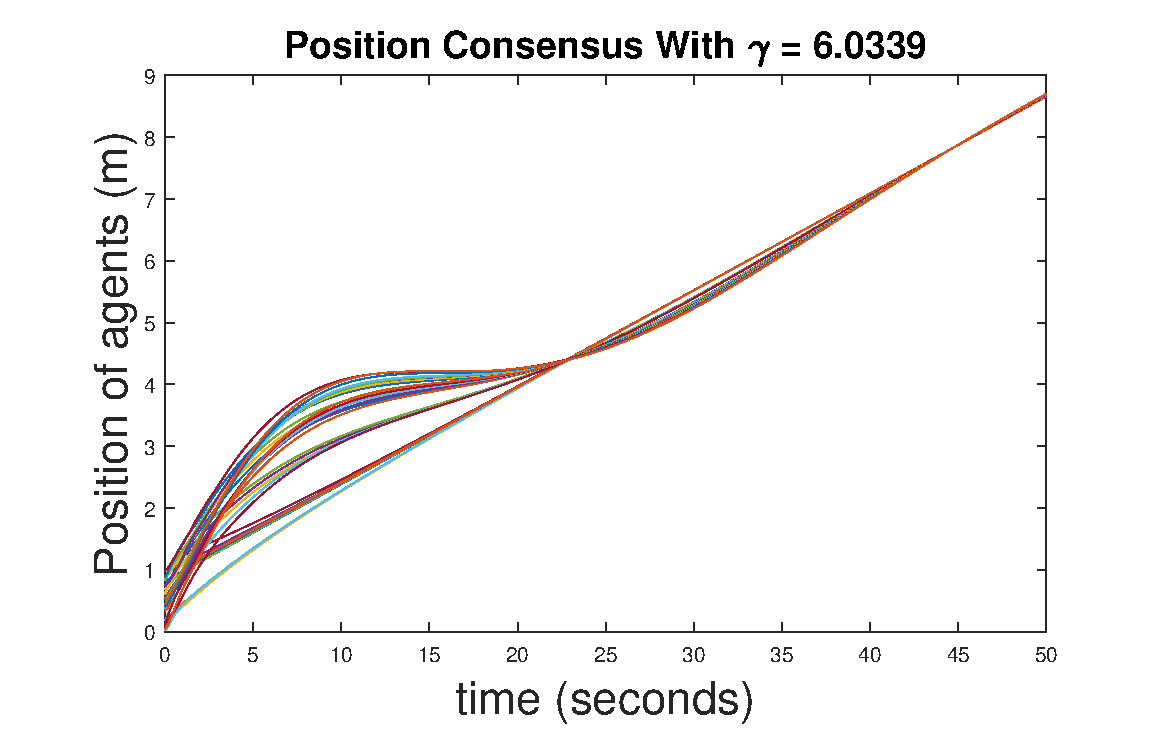
\includegraphics[width=0.75\textwidth,keepaspectratio]{2_Images/position_plot_for_theis.eps}
        %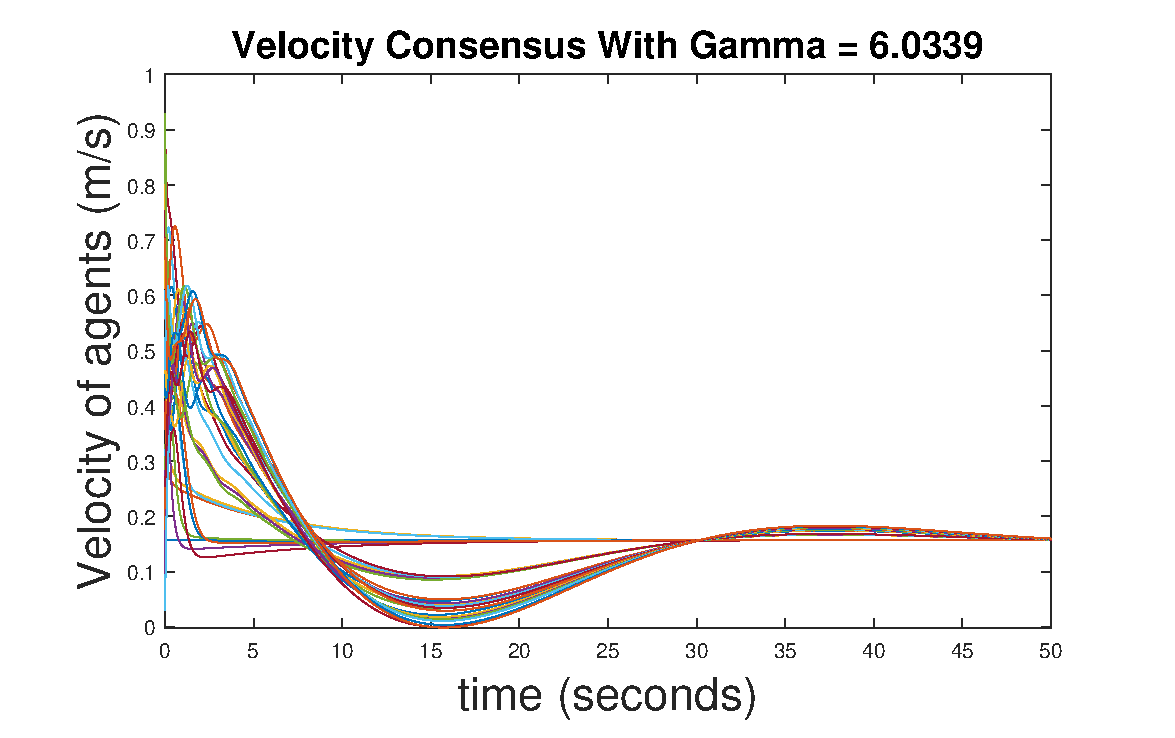
\includegraphics[width=0.75\textwidth,keepaspectratio]{2_Images/velocity_plot_for_theis.eps}
        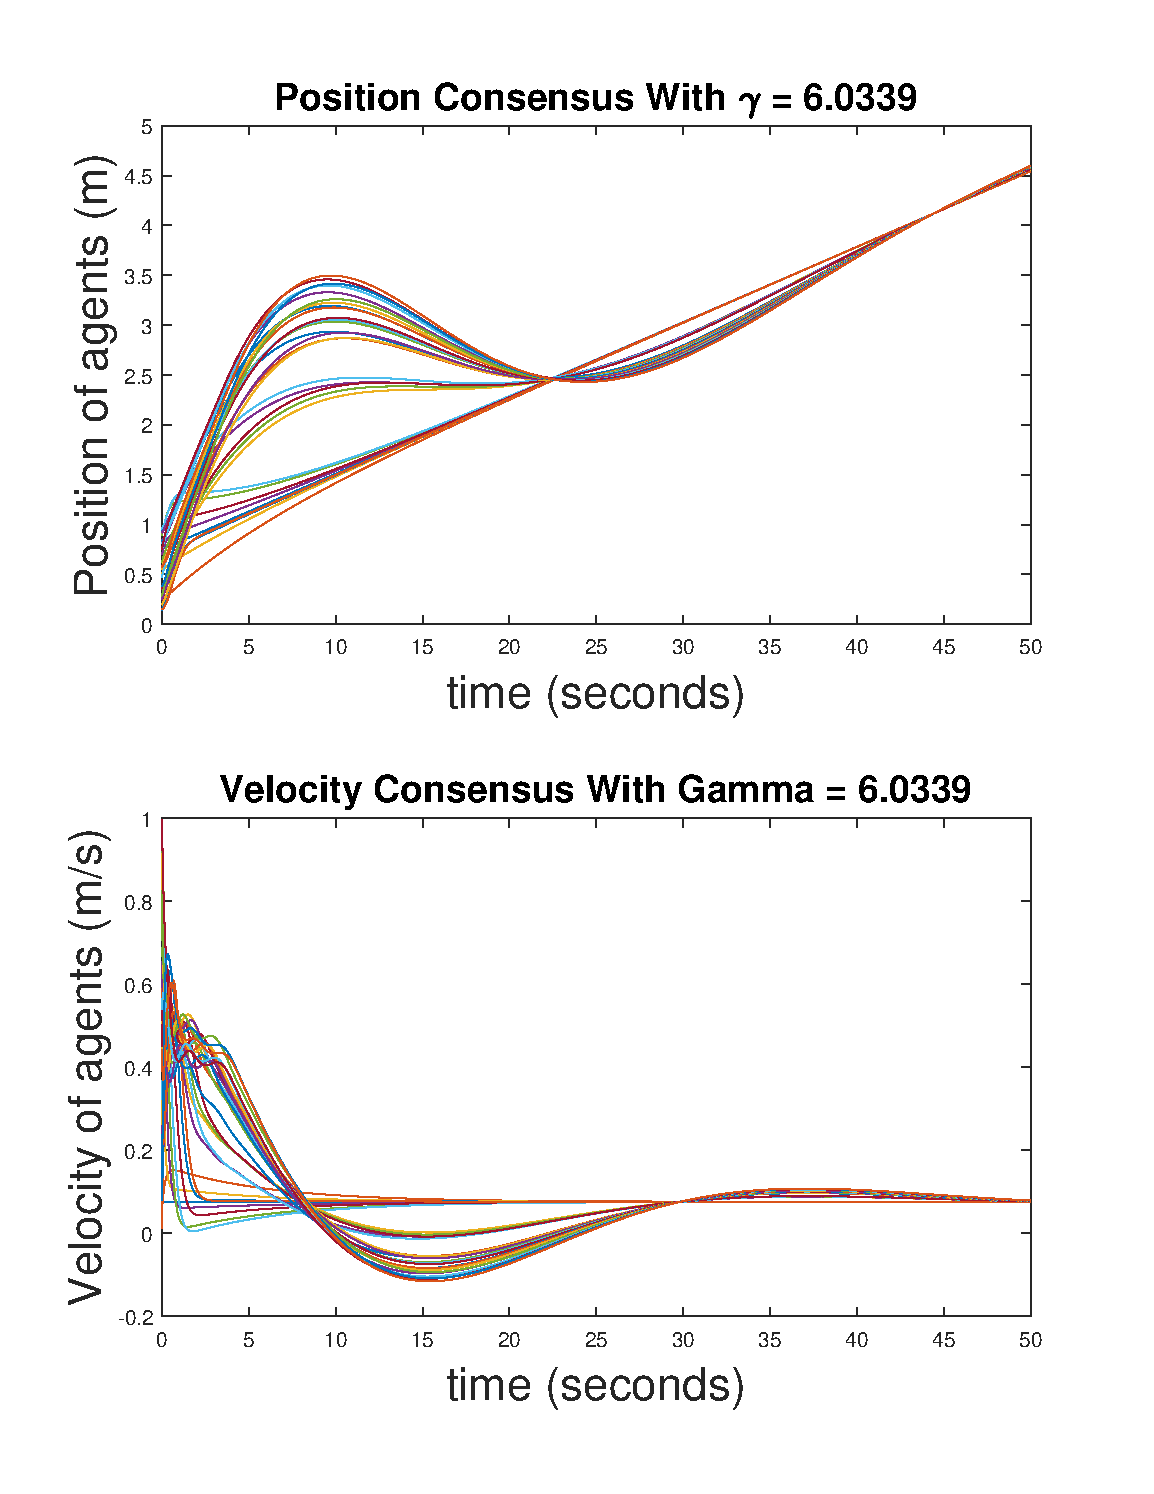
\includegraphics[width=0.75\textwidth,keepaspectratio]{2_Images/New_Stable.eps}
		\caption{Position and Velocity consensus in presence of two reverse edges where $x_1<x_2<y_1<y_2$}
		\label{Case3cconsensus}
	\end{figure}
    \begin{figure}[ht!]
    \centering
		%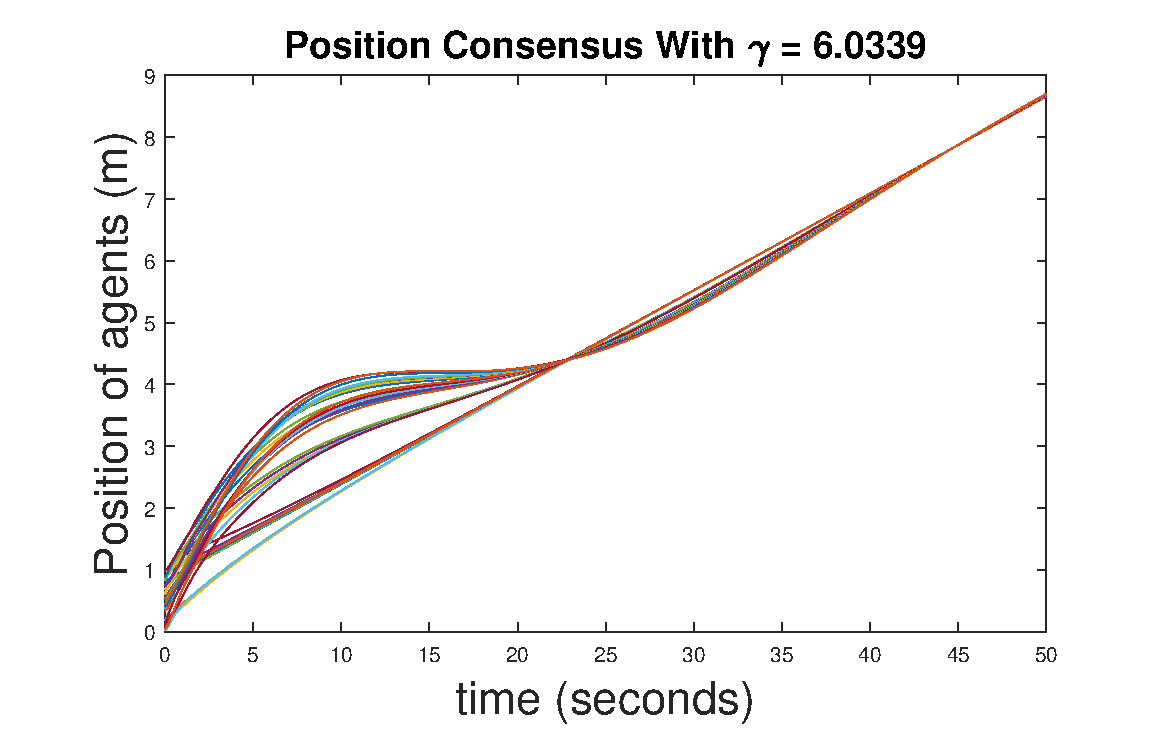
\includegraphics[width=0.75\textwidth,keepaspectratio]{2_Images/position_plot_for_theis.eps}
        %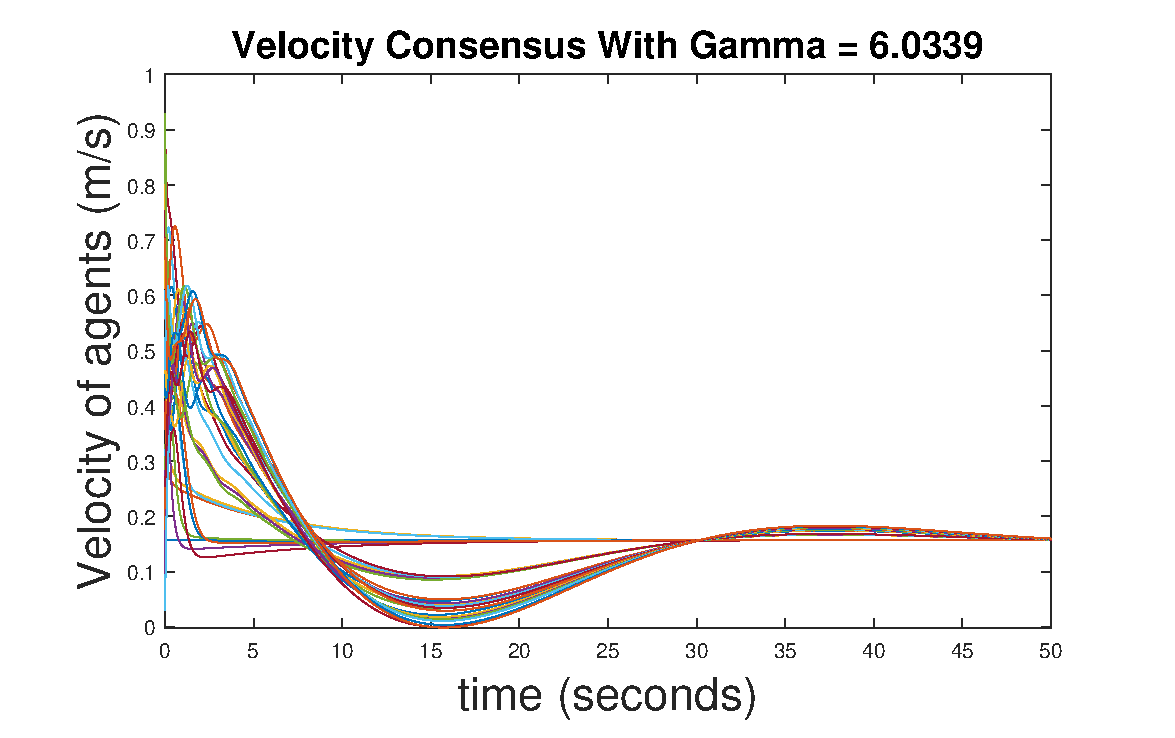
\includegraphics[width=0.75\textwidth,keepaspectratio]{2_Images/velocity_plot_for_theis.eps}
        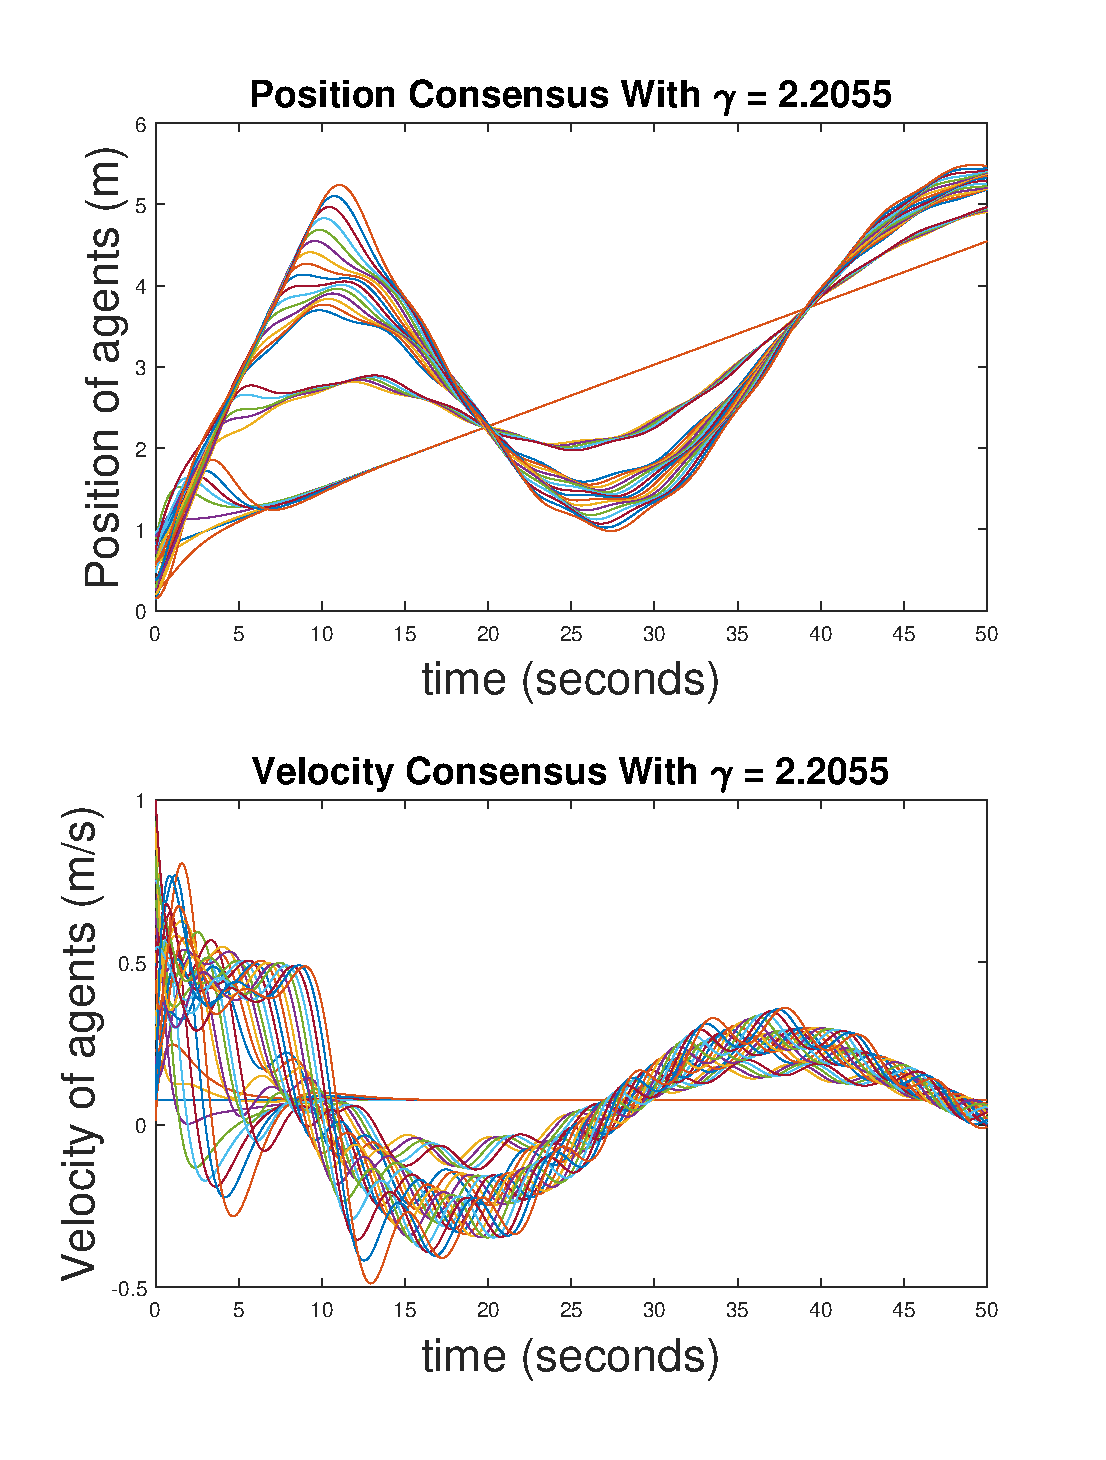
\includegraphics[width=0.75\textwidth,keepaspectratio]{2_Images/New_Unstable.eps}
		\caption{Consensus Breakdown in presence of two reverse edges where $x_1<x_2<y_1<y_2$}
		\label{Case3cconsensusBreakdown}
	\end{figure}

\section{Summary}\label{sec:ch_TRE_Summary}
In this chapter, we investigated the spectral impact of introducing dual reverse feedback edges across a directed chain network of double-integrator agents. The main findings and contributions of this chapter are summarized as follows:
\begin{itemize}
    \item \textbf{Exhaustive Topological Spectral Analysis:} We derived exact univariate characteristic polynomial equations across all six possible dual-loop spatial configurations (Cases 1–6) without imposing restrictive cycle-length or node-positioning assumptions.
    \item \textbf{Velocity Coupling Boundaries:} We proved that the dominant Laplacian eigenvalue $\lambda_2 = 1 - s_1$ is strictly governed by the unique real solution $s_1 \in (0,1)$ of the corresponding transformed polynomial. This real root dictates the exact non-negotiable lower bound on the velocity coupling gain ($\gamma \ge 1/\sqrt{1 - s_1}$) required to prevent dynamic divergence.
    \item \textbf{The Root-Node Loop Structural Singularity:} We formally established the Eigenvalue Shift Theorem (Theorem \ref{theo12}), proving that a loop of range $\ell$ alters $\ell+1$ eigenvalues when the root node is exterior ($x_1 > 1$), but affects only $\ell$ non-zero eigenvalues when the root node participates in loop formation ($x_1 = 1$).
    \item \textbf{Inherent Limitation of Global Polynomial Methods:} We proved that when $x_1 = 1$, standard polynomial methods collapse entirely, yielding the uninformative trivial solution $s_1 = 1 \implies \lambda_2 = 0$. This occurs because embedding the leader node in a feedback loop destroys its zero in-degree property ($d_{\text{in}, 1} > 0$), collapsing the leader-follower hierarchy and transforming all cycle nodes into co-equal root nodes.
\end{itemize}

The theoretical collapse of consensus, identified in Section 2.4, reveals a critical design issue for physical multi-agent networks: if an operational system has a fixed, predesigned velocity coupling gain $\gamma$ (or if a feedback loop enters the leader node $x_1 = 1$), traditional global spectrum re-computation fails to guarantee stability. 

To overcome these fundamental limitations, without requiring global network retuning or complete spectral evaluation of the Laplacian, Chapter \ref{ch:Guaranteed_Consensus} formulates a \textbf{decentralized, localized edge-weight perturbation framework}. By leveraging Gershgorin's Disc Theorem, sub-block shifts, local Node-Scaling, Edge-Scaling, and Root-Locus based tuning algorithms are synthesized to restore second-order consensus and resolve the root-node loop singularity under fixed coupling constraints.
%\chapter[Guaranteed Consensus of Double-Integrator Systems in the Presence of Directed Cycles]{Guaranteed Consensus of Double-Integrator Systems in the Presence of Directed Cycles\footnote{The core theoretical algorithms and formulations in this chapter are derived in part from the author's published work in the \emph{Proceedings of the American Control Conference (ACC)}. This chapter expands upon those preliminary manuscripts by providing unified proofs, comprehensive sub-block matrix extensions, and root-locus design frameworks.}}\label{ch:Guaranteed_Consensus}
\chapter[Guaranteed Consensus in Directed Cyclic Networks]{Guranteed Consensus of Double-Integrators in the Presence of Directed Cycles\footnote{The theoretical formulations of the problems and the algorithms have some overlap with the author's published work in the \emph{Proceedings of the American Control Conference (ACC) 2023}. This chapter expands upon the preliminary results by providing detailed proofs, comprehensive sub-block matrix extensions, and root-locus based design frameworks.}}\label{ch:Guaranteed_Consensus}

\section{Introduction}\label{sec:ch_GC_intro_Guaranteed_Consensus}
As established in Chapters \ref{ch:intro} and \ref{ch:TwoReverseEdges}, second-order consensus over directed graphs exhibits a fundamental vulnerability: the introduction of reverse feedback channels forms directed cycles. These cycles introduce complex-conjugate eigenvalues into the graph Laplacian spectrum $\sigma(\mathcal{L})$, inducing phase lag between position alignment and velocity damping. As proven by Ren and Atkins \cite{ren2005second} and Yu et al. \cite{yu2010some}, second-order consensus breaks down completely unless the velocity coupling parameter $\gamma$ exceeds a critical lower threshold dictated by the Laplacian spectrum:
\begin{equation}\label{eq:ch_GC_yu_threshold_recap}
    \gamma > \max_{i \in \{2, \dots, N\}} \frac{|\mathfrak{Im}(\lambda_i)|}{|\lambda_i|} \sqrt{\frac{1}{\mathfrak{Re}(\lambda_i)}}
\end{equation}
In practical hierarchical networks— such as organizational swarms, industrial automated guided vehicles (AGVs), or multi-tiered power grids— reverse communication links frequently arise due to localized feedback, spatial proximity, or status reporting. When a reverse edge is added to an operational network with a predesigned, fixed coupling parameter $\gamma$, condition \eqref{eq:ch_GC_yu_threshold_recap} is easily violated, leading to severe dynamic instability.
\begin{figure}[ht!]
	\centering
	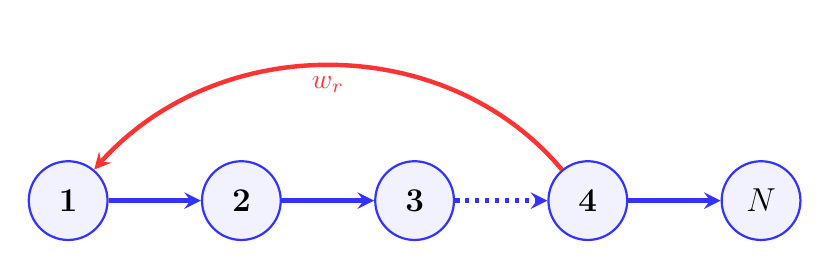
\begin{tikzpicture}[node distance=2.2cm, state/.style={circle, draw=blue!80, fill=blue!5, thick, minimum size=1.0cm, font=\large\bfseries}]
		\node[state] (1) {1};
		\node[state] (2) [right of=1] {2};
		\node[state] (3) [right of=2] {3};
		\node[state] (4) [right of=3] {4};
		\node[state] (5) [right of=4] {$N$};
		
		\path [->, >=stealth, ultra thick, blue!80] (1) edge (2);
		\path [->, >=stealth, ultra thick, blue!80] (2) edge (3);
		\path [->, >=stealth, ultra thick, blue!80] (3) edge[dotted] (4);
		\path [->, >=stealth, ultra thick, blue!80] (4) edge (5);
		\path [->, >=stealth, ultra thick, red!80] (4) edge[bend right=50] node[below] {$w_r$} (1);
	\end{tikzpicture}
	\caption{Directed chain network with a reverse feedback edge entering the leader node ($x_1 = 1$), forming a root-node loop.}
	\label{fig:LeaderCycleNetwork}
\end{figure}
\begin{figure}[ht!]
	\centering
	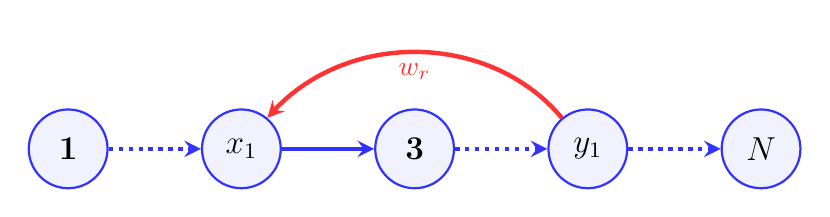
\begin{tikzpicture}[node distance=2.2cm, state/.style={circle, draw=blue!80, fill=blue!5, thick, minimum size=1.0cm, font=\large\bfseries}]
		\node[state] (1) {1};
		\node[state] (2) [right of=1] {$x_1$};
		\node[state] (3) [right of=2] {3};
		\node[state] (4) [right of=3] {$y_1$};
		\node[state] (5) [right of=4] {$N$};
		
		\path [->, >=stealth, ultra thick, blue!80] (1) edge[dotted] (2);
		\path [->, >=stealth, ultra thick, blue!80] (2) edge (3);
		\path [->, >=stealth, ultra thick, blue!80] (3) edge[dotted] (4);
		\path [->, >=stealth, ultra thick, blue!80] (4) edge[dotted] (5);
		\path [->, >=stealth, ultra thick, red!80] (4) edge[bend right=50] node[below] {$w_r$} (2);
	\end{tikzpicture}
	\caption{Directed chain network with a reverse feedback edge strictly exterior to the leader node ($x_1 > 1$).}
	\label{fig:LeaderlessCycleNetwork}
\end{figure}
In Chapter \ref{ch:TwoReverseEdges}, we established two major analytical barriers to mitigating this breakdown:
\begin{itemize}
    \item \textbf{High Computational and Communication Overhead of Global Retuning:} Restoring stability by adjusting $\gamma$ globally requires every agent in the network to access the updated global Laplacian spectrum $\sigma(\mathcal{L})$, destroying the decentralized nature of the network protocol.
    \item \textbf{The Root-Node Loop Structural Singularity:} When a reverse edge enters the root/leader node itself ($x_1 = 1$, as shown in Figure \ref{fig:LeaderCycleNetwork}), standard characteristic polynomial methods collapse ($s_1 = 1 \implies \lambda_2 = 0$). The leader node loses its zero in-degree property ($d_{\text{in}, 1} > 0$), destroying the leader-follower hierarchy and converting every node in the loop into an equivalent root node.
\end{itemize}

\subsection*{Summary of Chapter Contributions}
To resolve these challenges, this chapter synthesizes a suite of \textbf{fully localized control remedies} that guarantee second-order consensus under fixed global coupling parameters $\gamma$. The specific contributions are:
\begin{enumerate}
    \item \textbf{Decentralized Gershgorin--Based Perturbation Framework (Leader -- Exterior Loops):} For directed cycles that do not contain the leader/root node ($x_1 > 1$, Figure \ref{fig:LeaderlessCycleNetwork}), we formulate \textbf{Node-Scaling, Edge-Scaling, and Combined-Scaling} algorithms. By constructing optimal Arithmetic Progressions (AP) of Gershgorin column discs, we guarantee that the minimum real eigenvalue component satisfies $\mathfrak{Re}(\lambda_2) \ge 1/\gamma^2$, ensuring consensus through localized gains confined strictly to loop agents and edges.
    \item \textbf{Resolution of the Root-Node Loop Singularity via Complementary Root-Locus:} For directed cycles that incorporate the leader node ($x_1 = 1$, Figure \ref{fig:LeaderCycleNetwork}), where Gershgorin-based methods fail, we formulate a complementary root-locus control framework. By modeling loop gain shifts via $G(s) = \frac{\beta\{(s-\alpha)^\ell - (-\alpha)^\ell\}}{s(s-\alpha)^\ell}$, we derive precise gain bounds on $\alpha$ and $\beta$ that guarantee stability.
    \item \textbf{Equal-Weight Cyclic Pursuit Synthesis:} To prevent edge-weakening under root-node loops, we derive an exact closed-form single-gain threshold ($\alpha \ge \frac{\cot^2(\pi/(\ell+1))}{2\gamma^2}$) based on cyclic pursuit, guaranteeing consensus while maintaining equal edge weights across all agents in the directed cycle.
\end{enumerate}
\section{Mathematical Preliminaries and Problem Formulation} \label{sec:ch_GC_prelims}
This section formalizes the network state equations, graph-theoretic structures, and fundamental mathematical lemmas required to develop localized perturbation remedies.
\subsection{System Dynamics and Laplacian Matrix Partitions}
Consider an $N$-agent multi-agent system interacting over a directed graph $\mathcal{G} = (\mathcal{V}_g, \mathcal{E}_g, \mathcal{W}_g)$. Recall from Section \ref{sec:ch_TRE_Prelims} that the translational motion of agent $i \in \{1, 2, \dots, N\}$ in $d$-dimensional space is governed by double-integrator dynamics $\dot{p}_i = v_i, \dot{v}_i = u_i$. Under the local control protocol \eqref{eq:ch_TRE_agent_wise}:
\begin{equation} \label{eq:ch_GC_control_law}
	u_i(t) = -\sum_{j=1}^{N} w_{ij} \left[ (p_i(t) - p_j(t)) + \gamma (v_i(t) - v_j(t)) \right], \quad i \in \{1, 2, \dots, N\}
\end{equation}
where $w_{ij}$ is the $(i,j)$-th entry of the weighted adjacency matrix $\mathcal{W}_g$, and $\gamma > 0$ is the predesigned, fixed global velocity coupling parameter. Stacking composite states into $\mathcal{X}(t) \coloneqq [p^T(t), v^T(t)]^T \in \mathbb{R}^{2Nd}$, the global system evolves according to $\dot{\mathcal{X}}(t) = (\hat{\mathcal{L}} \otimes I_d) \mathcal{X}(t)$, where:
\begin{equation}\label{eq:ch_GC_hat_laplacian}
	\hat{\mathcal{L}} = \begin{bmatrix} 0_{N \times N} & I_N \\ -\mathcal{L} & -\gamma \mathcal{L} \end{bmatrix} \in \mathbb{R}^{2N \times 2N}
\end{equation}

When the interaction graph is a nominal $N$-node directed chain indexed by topological ordering (Definition \ref{def:ch_TRE_chaindigraph}), the graph Laplacian $\mathcal{L}$ is strictly lower triangular. When a reverse edge of weight $w_r > 0$ is inserted from tail node $y_1$ to head node $x_1$ ($y_1 > x_1$), forming a cycle of range $\ell = y_1 - x_1$, the structure of $\mathcal{L}$ depends on whether the leader node ($x_1 = 1$) is involved:

1. Leader-Exterior Loop ($x_1 > 1$, Figure \ref{fig:LeaderlessCycleNetwork}):
   \begin{equation} \label{eq:ch_GC_OriginalLaplacian}
   	\mathcal{L}_{\text{ext}} = \begin{bmatrix}
   		\mathcal{L}_1 & 0 & 0 \\
   		* & \mathcal{C} + \mathcal{L}_{\text{re}} & 0 \\
   		* & * & \mathcal{L}_2
   	\end{bmatrix}
   \end{equation}
   where $\mathcal{L}_1 \in \mathbb{R}^{(x_1-1) \times (x_1-1)}$ and $\mathcal{L}_2 \in \mathbb{R}^{(N-y_1) \times (N-y_1)}$ are lower triangular sub-matrices corresponding to unperturbed chain segments, $\mathcal{C} \in \mathbb{R}^{(\ell+1) \times (\ell+1)}$ represents the nominal sub-chain, and $\mathcal{L}_{\text{re}}$ captures the additive perturbation due to the reverse edge:
   \begin{equation}\label{eq:ch_GC_ReverseEdgeMatrix}
   	\mathcal{L}_{\text{re}} = \begin{bmatrix}
   		w_r & 0 & \dots & 0 & -w_r \\
   		0 & 0 & \dots & 0 & 0 \\
   		\vdots & \vdots & \ddots & \vdots & \vdots \\
   		0 & 0 & \dots & 0 & 0
   	\end{bmatrix} \in \mathbb{R}^{(\ell+1) \times (\ell+1)}
   \end{equation}

2. Root-Node Loop ($x_1 = 1$, Figure \ref{fig:LeaderCycleNetwork}):
   \begin{equation} \label{eq:ch_GC_OriginalLaplacianleader}
   	\mathcal{L}_{\text{root}} = \begin{bmatrix}
   		\mathcal{C} + \mathcal{L}_{\text{re}} & 0 \\
   		* & \mathcal{L}_2
   	\end{bmatrix}
   \end{equation}
   where $\mathcal{C} + \mathcal{L}_{\text{re}} \in \mathbb{R}^{(\ell+1) \times (\ell+1)}$ is a circulant-like block containing the zero eigenvalue $\lambda_1 = 0$.

Because of the block lower-triangular structure in \eqref{eq:ch_GC_OriginalLaplacian} and \eqref{eq:ch_GC_OriginalLaplacianleader}, the non-zero complex spectrum of $\mathcal{L}$ is determined entirely by the sub-block $\mathcal{C} + \mathcal{L}_{\text{re}}$.

\subsection{Foundational Stability Criteria and Problem Statement}

Recall from Lemma \ref{lem:ch_TRE_sufficiencyren} and Equation \eqref{eq:ch_TRE_DubeyBound} that second-order consensus is guaranteed if the non-zero Laplacian spectrum satisfies:
\begin{equation}\label{eq:ch_GC_dubey_bound}
    \mathfrak{Re}(\lambda_i) \ge \mathfrak{Re}(\lambda_2) \ge \frac{1}{\gamma^2}, \quad \forall i \in \{2, \dots, N\}
\end{equation}
Condition \eqref{eq:ch_GC_dubey_bound} provides a clear goal to be met: to guarantee consensus under a fixed global coupling gain $\gamma$, local control gain readjustments must shift the spectrum of $\mathcal{C} + \mathcal{L}_{\text{re}}$ so that every non-zero eigenvalue resides to the right of the vertical line $\mathfrak{Re}(z) = 1/\gamma^2$ in the complex plane.

This immediately leads to the core problem addressed in this chapter.

\begin{problem}\label{prob:ch_GC_main_problem}
Consider an $N$-node directed chain of double-integrator agents operating under protocol \eqref{eq:ch_GC_control_law} with a fixed, predesigned velocity coupling parameter $\gamma > 0$. Suppose a reverse feedback edge is added, forming a directed cycle of range $\ell \coloneqq y_1 - x_1$. Synthesize localized node/edge parameter tuning strategies confined strictly to the agents and edges participating in (or adjacent to) the cycle such that second-order consensus is guaranteed without adjusting global parameters ($\gamma$) or requiring all the agents to access the global Laplacian spectrum $\sigma(\mathcal{L})$.
\end{problem}

\subsection{Mathematical Toolset}
To resolve Problem \ref{prob:ch_GC_main_problem}, we utilize Gershgorin's Disc Theorem along with three key algebraic/geometric propositions.
\begin{theo}[Gershgorin's Disc Theorem \cite{horn2012matrix}]\label{thm:ch_GC_GershgorinDiscTheorem}
Let $A = [a_{ij}] \in \mathbb{R}^{n \times n}$ be a square matrix. For each column $j \in \{1, 2, \dots, n\}$, define the deleted column-sum radius $R_j(A) \coloneqq \sum_{i=1, i \neq j}^{n} |a_{ij}|$. Associated with column $j$, define the closed Gershgorin disc $\mathfrak{D}_j(A)$ in the complex plane $\mathbb{C}$:
\begin{equation}
	\mathfrak{D}_j(A) \coloneqq \left\{ z \in \mathbb{C} : |z - a_{jj}| \le R_j(A) \right\}
\end{equation}
All eigenvalues $\lambda \in \sigma(A)$ lie within the union of these $n$ column discs: $\sigma(A) \subset \bigcup_{j=1}^{n} \mathfrak{D}_j(A)$. By matrix transposition ($\sigma(A) = \sigma(A^T)$), identical statements hold for row-sum radii.
\end{theo}
\begin{proposition}[Polynomial Root Reflection]\label{prop:ch_GC_polynomialreflection}
If $f(x) = \sum_{i=0}^{n} a_i x^i$ is a polynomial with real coefficients $a_i \in \mathbb{R}$ having roots $x_i \in \mathbb{C}$, then the polynomial $f(-x)$ has roots given by $-x_i^*$, where $(\cdot)^*$ denotes complex conjugation.
\end{proposition}
\begin{proof}
Since $a_i \in \mathbb{R}$, complex roots of $f(x)$ occur in conjugate pairs. Factoring $f(x)$ into $m$ real linear factors and $(n-m)/2$ quadratic real factors:
\begin{equation}\label{eq:f_pos}
	f(x) = \prod_{i=1}^{m} (x - x_i) \cdot \prod_{k=1}^{\frac{n-m}{2}} (p_k x^2 + q_k x + r_k)
\end{equation}
Substituting $x \to -x$ yields:
\begin{equation}\label{eq:f_neg}
	f(-x) = (-1)^m \prod_{i=1}^{m} (x + x_i) \cdot \prod_{k=1}^{\frac{n-m}{2}} (p_k x^2 - q_k x + r_k)
\end{equation}
For any real root $x_i \in \mathbb{R}$, $-x_i = -x_i^*$. For a quadratic factor $g(y) = p y^2 + q y + r$ with complex conjugate roots $y_1, y_1^* = \frac{-q \mp j \sqrt{4pr - q^2}}{2p}$, the roots of $g(-y) = p y^2 - q y + r$ are $z_1, z_1^* = \frac{q \mp j \sqrt{4pr - q^2}}{2p} = -y_1^*, -y_1$. Thus, all roots of $f(-x)$ are located at $-x_i^*$.
\end{proof}

\begin{proposition}[Optimal Arithmetic Progression for Disc Separation]\label{prop:ch_GC_AP_optimization}
\leavevmode\par\noindent
Let $a, b \in \mathbb{R}$ with $a > b$. Consider a sequence of $n$ numbers satisfying:
\begin{equation}\label{eq:ch_GC_sequence}
	a > x_1 > x_2 > \dots > x_n > b
\end{equation}
Define the $n+1$ adjacent differences $d_1 = a - x_1$, $d_i = x_{i-1} - x_i$ for $i \in \{2, \dots, n\}$, and $d_{n+1} = x_n - b$. The cost function $J \coloneqq \min\limits_{j \in \{1, \dots, n+1\}} d_j$ is maximized if and only if the sequence $\{x_i\}$ forms an Arithmetic Progression (AP) with common difference:
\begin{equation}\label{eq:ch_GC_AP_diff}
	d = \frac{a - b}{n+1}
\end{equation}
\end{proposition}
\begin{proof}
Let Series 1 be the sequence where elements are in AP with common difference $d = \frac{a-b}{n+1}$, giving $d_i = d ~\forall~ i$. Let Series 2 be any non-AP sequence with differences $d_i'$. Let $d_k' = \min_i (d_i')$. We can write $d_i' = d_k' + r_i$, where $r_i \ge 0$, with strict inequality holding for at least one $i$.
Summing all differences for Series 2:
\begin{equation*}
	\sum_{i=1}^{n+1} d_i' = a - b = (n+1)d_k' + X, \quad \text{where } X = \sum_{i=1}^{n+1} r_i > 0
\end{equation*}
For Series 1, $\sum_{i=1}^{n+1} d_i = a - b = (n+1)d$. Equating both expressions yields $(n+1)d_k' + X = (n+1)d \implies X = (n+1)(d - d_k')$. Since $X > 0$, it follows directly that $d > d_k'$. Thus, the maximum possible minimum separation is uniquely achieved when the sequence forms an arithmetic progression.
\end{proof}
\begin{proposition}[Geometric Angle Invariance of Parallel Chords]\label{prop:ch_GC_chord_geometry}
\leavevmode\par\noindent
Consider a circle of radius $a > 0$ centered at $(a,0)$ in the complex plane, tangent to the imaginary axis at the origin (Figure \ref{fig:chord}). Let $AA_1$ and $BB_1$ be vertical chords parallel to the imaginary axis with real $x$-intercepts $x_1$ and $x_2$, respectively. If $x_2 > x_1 > 0$ (i.e., chord $AA_1$ is strictly closer to the origin than $BB_1$), then the ray angles $\theta_1 = \angle A_1 O C$ and $\theta_2 = \angle B_1 O C$ subtended at the origin satisfy:
\begin{equation}
	\theta_1 > \theta_2
\end{equation}
\end{proposition}

\begin{proof}
The circle equation is $(x-a)^2 + y^2 = a^2 \implies x^2 + y^2 = 2ax$. For points $A_1 = (x_1, y_1)$ and $B_1 = (x_2, y_2)$ lying on the circle, $x_1^2 + y_1^2 = 2ax_1$ and $x_2^2 + y_2^2 = 2ax_2$. The cosine of the subtended angle $\theta_1$ is:
\begin{equation}
	\cos(\theta_1) = \frac{x_1}{\sqrt{x_1^2 + y_1^2}} = \frac{x_1}{\sqrt{2ax_1}} = \frac{\sqrt{x_1}}{\sqrt{2a}}
\end{equation}
Similarly, $\cos(\theta_2) = \frac{\sqrt{x_2}}{\sqrt{2a}}$. Since $x_2 > x_1 > 0$, $\sqrt{x_2} > \sqrt{x_1} \implies \cos(\theta_2) > \cos(\theta_1)$. Because $\cos(\theta)$ is strictly decreasing on $\theta \in [0, \pi/2]$, $\cos(\theta_2) > \cos(\theta_1)$ implies $\theta_1 > \theta_2$.
\end{proof}

\begin{figure}[ht!]
	\centering
	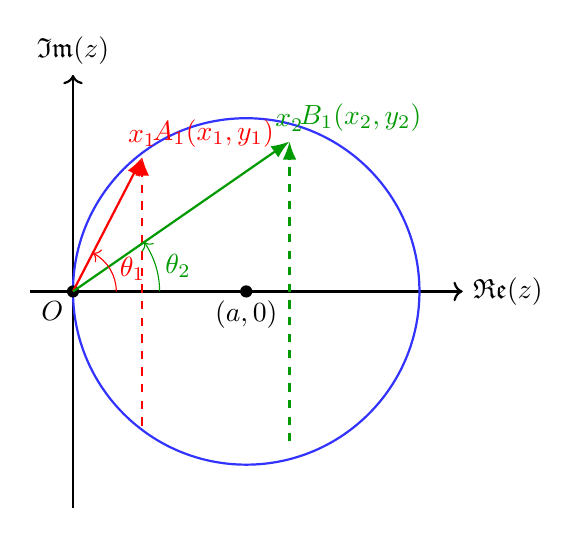
\begin{tikzpicture}[scale=1.1]
		\draw[->, thick] (-0.5,0) -- (4.5,0) node[right] {$\mathfrak{Re}(z)$};
		\draw[->, thick] (0,-2.5) -- (0,2.5) node[above] {$\mathfrak{Im}(z)$};
		\draw[thick, blue!80] (2,0) circle (2cm);
		\fill (2,0) circle (2pt) node[below] {$(a,0)$};
		\fill (0,0) circle (2pt) node[below left] {$O$};
		
		\draw[dashed, red, thick] (0.8,-1.549) -- (0.8,1.549) node[above] {$x_1$};
		\draw[dashed, green!60!black, thick] (2.5,-1.732) -- (2.5,1.732) node[above] {$x_2$};
		
		\draw[thick, red] (0,0) -- (0.8,1.549) node[above right] {$A_1(x_1,y_1)$};
		\draw[thick, green!60!black] (0,0) -- (2.5,1.732) node[above right] {$B_1(x_2,y_2)$};
		
		\draw[red, ->] (0.5,0) arc (0:62.68:0.5) node[midway, right] {$\theta_1$};
		\draw[green!60!black, ->] (1.0,0) arc (0:34.72:1.0) node[midway, right] {$\theta_2$};
	\end{tikzpicture}
	\caption{Geometric relationship between parallel chord $x$-intercepts ($x_1 < x_2$) and subtended ray angles ($\theta_1 > \theta_2$) for a circle tangent to the imaginary axis.}
	\label{fig:chord}
\end{figure}

\section{Decentralized Control Strategies for Loops excluding Leader/Root ($x_1 > 1$)}
When the root/leader node is external to the loop ($x_1 > 1$), Node 1 retains its zero in-degree property ($d_{\text{in},1} = 0$). We present three Gershgorin-based scaling strategies that guarantee consensus under fixed global coupling parameters $\gamma$.

\subsection{Node-Based Scaling Strategy}\label{sec:NodeMethod}
In Node-Based Scaling, the control law $u_i(t)$ of each agent participating in the cycle ($i \in \{x_1, x_1+1, \dots, y_1\}$) is scaled by a local positive scalar $p_{i-x_1+1} > 0$. Stacking these factors into a diagonal matrix $P = \text{diag}(p_1, p_2, \dots, p_{\ell+1}) \in \mathbb{R}^{(\ell+1) \times (\ell+1)}$, we construct the block diagonal network scaling matrix $\mathcal{D} \in \mathbb{R}^{N \times N}$:
\begin{equation} \label{eq:ch_GC_MatrixD}
	\mathcal{D} = \begin{bmatrix}
		I_{x_1-1} & 0 & 0 \\
		0 & P & 0 \\
		0 & 0 & I_{N-y_1}
	\end{bmatrix}
\end{equation}
\begin{figure}[ht!]
	\centering
	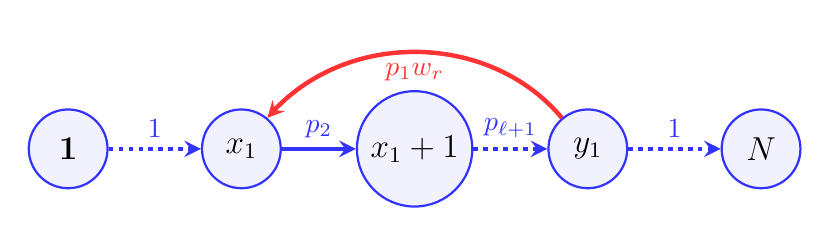
\begin{tikzpicture}[node distance=2.2cm, state/.style={circle, draw=blue!80, fill=blue!5, thick, minimum size=1.0cm, font=\large\bfseries}]
		\node[state] (1) {1};
		\node[state] (2) [right of=1] {$x_1$};
		\node[state] (3) [right of=2] {$x_1+1$};
		\node[state] (4) [right of=3] {$y_1$};
		\node[state] (5) [right of=4] {$N$};
		
		\path [->, >=stealth, ultra thick, blue!80] (1) edge[dotted] node[above] {$1$} (2);
		\path [->, >=stealth, ultra thick, blue!80] (2) edge node[above] {$p_2$} (3);
		\path [->, >=stealth, ultra thick, blue!80] (3) edge[dotted] node[above] {$p_{\ell+1}$} (4);
		\path [->, >=stealth, ultra thick, blue!80] (4) edge[dotted] node[above] {$1$} (5);
		\path [->, >=stealth, ultra thick, red!80] (4) edge[bend right=50] node[below] {$p_1 w_r$} (2);
	\end{tikzpicture}
	\caption{Node-Scaled Network Topology, where every incoming edge to node $i$ in the cycle is scaled by local scalar $p_{i-x_1+1}$.}
	\label{fig:NodeScaledNetwork}
\end{figure}

Premultiplying the modified Laplacian $\mathcal{L}_{\text{ext}}$ in \eqref{eq:ch_GC_OriginalLaplacian} by $\mathcal{D}$ yields the node-scaled equivalent Laplacian $\mathcal{L}_{\text{eq}} = \mathcal{D} \mathcal{L}_{\text{ext}}$:
\begin{equation} \label{eq:ch_GC_LaplacianEqNode}
	\mathcal{L}_{\text{eq}} = \begin{bmatrix}
		\mathcal{L}_1 & 0 & 0 \\
		* & P(\mathcal{C} + \mathcal{L}_{\text{re}}) & 0 \\
		* & * & \mathcal{L}_2
	\end{bmatrix}
\end{equation}
Defining $\tilde{P} \coloneqq P(\mathcal{C} + \mathcal{L}_{\text{re}}) \in \mathbb{R}^{(\ell+1) \times (\ell+1)}$, for an unweighted nominal chain with unit reverse edge ($w_r = 1$), $\tilde{P}$ takes the explicit tridiagonal-circulant form:
\begin{equation}\label{eq:ch_GC_NSChainLoop}
	\tilde{P} = \begin{bmatrix}
		2p_1  & 0 & 0 & \dots & 0 & -p_1 \\
		-p_2 & p_2 & 0 & \dots & 0 & 0 \\
		0 & -p_3 & p_3 & \dots & 0 & 0 \\
		\vdots & \vdots & \ddots & \ddots & \vdots & \vdots \\
		0 & 0 & \dots & -p_{\ell} & p_{\ell} & 0 \\
		0 & 0 & \dots & 0 & -p_{\ell+1} & p_{\ell+1}
	\end{bmatrix}
\end{equation}

Applying Gershgorin's Disc Theorem (Theorem \ref{thm:ch_GC_GershgorinDiscTheorem}) to the columns of $\tilde{P}$, column $j=1$ centered at $2p_1$ has radius $R_1 = p_2$. Columns $j \in \{2, \dots, \ell\}$ centered at $p_j$ have radii $R_j = p_{j+1}$. Column $j=\ell+1$ centered at $p_{\ell+1}$ has radius $R_{\ell+1} = p_1$. 

To guarantee that all column discs lie strictly in the open right half-plane $\mathfrak{Re}(z) > 0$, the center of each disc must strictly exceed its radius:
\begin{equation}\label{eq:ch_GC_NSInequality}
	2p_1 > p_2 > p_3 > \dots > p_{\ell+1} > p_1
\end{equation}

The left boundary of disc $j$ cuts the real axis at distance $d_j$ from the origin: $d_1 = 2p_1 - p_2$, $d_j = p_j - p_{j+1}$ for $j \in \{2, \dots, \ell\}$, and $d_{\ell+1} = p_{\ell+1} - p_1$. The minimum real separation across all discs is $J = \min_j (d_j)$. By Proposition \ref{prop:ch_GC_AP_optimization}, $J$ is maximized if and only if the centers $\{2p_1, p_2, \dots, p_{\ell+1}, p_1\}$ form an Arithmetic Progression (AP) with common difference:
\begin{equation}\label{eq:ch_GC_node_diff}
	d = \frac{2p_1 - p_1}{\ell + 1} = \frac{p_1}{\ell + 1}
\end{equation}

\begin{figure}[ht!]
	\centering
	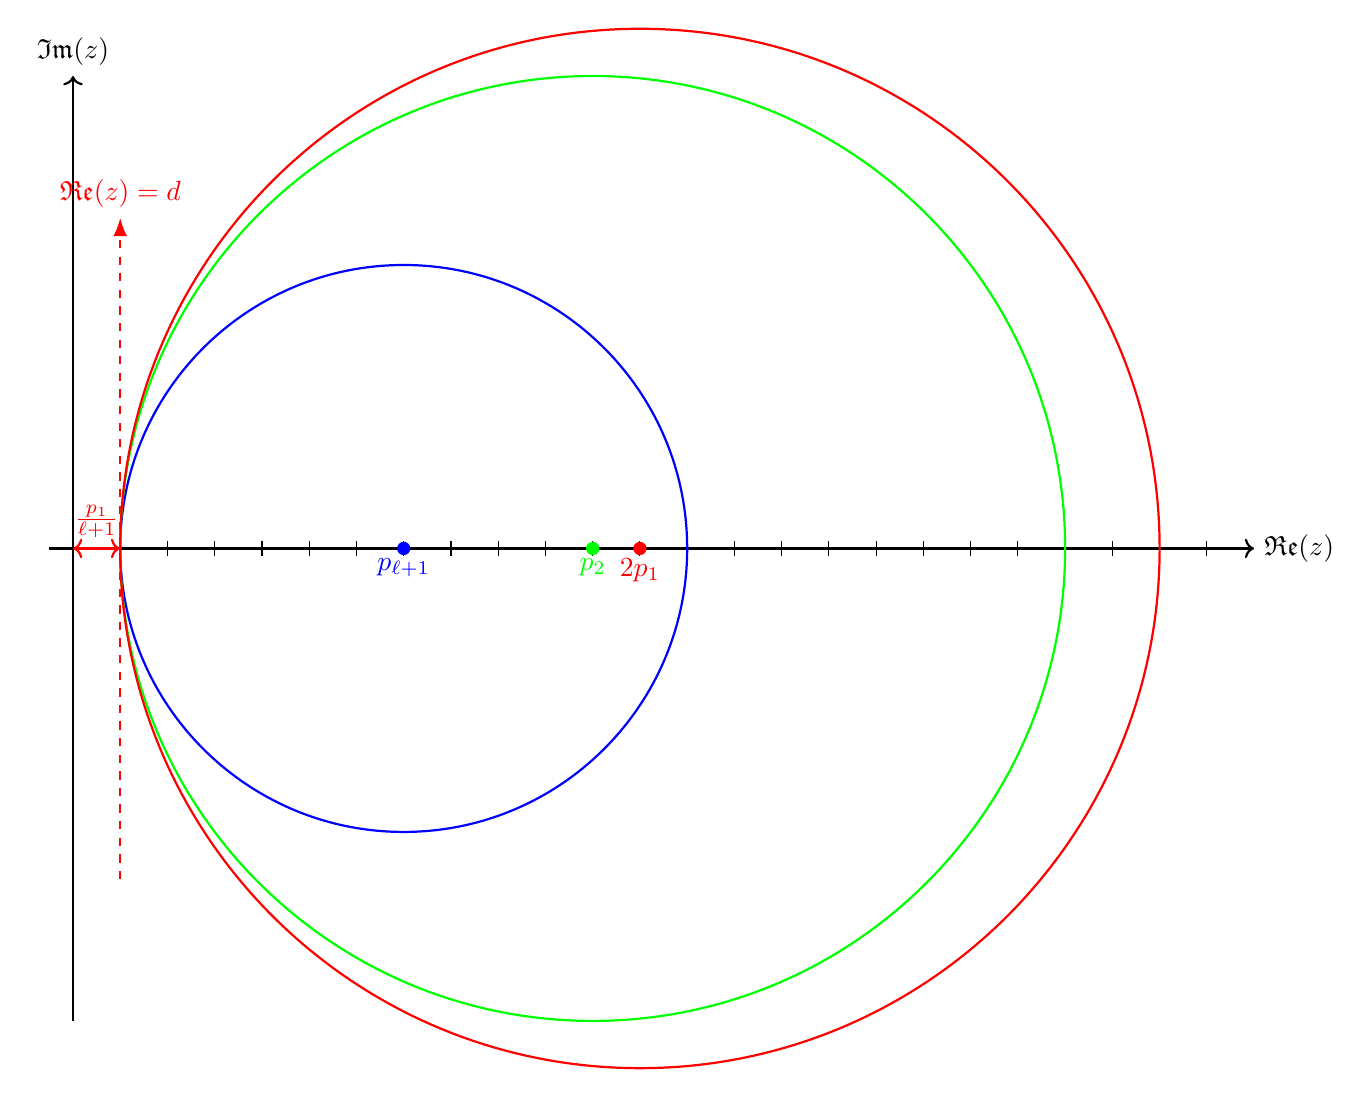
\begin{tikzpicture}[scale=0.3]
		\draw[->, thick] (-1,0) -- (50,0) node[right] {$\mathfrak{Re}(z)$};
		\draw[->, thick] (0,-20) -- (0,20) node[above] {$\mathfrak{Im}(z)$};
        \foreach \x in {2, 4, 6, 8, 10, 12, 14, 16, 18, 20, 22, 24, 26, 28, 30, 32, 34, 36, 38, 40, 42, 44, 46, 48}
		\draw[-] (\x, -0.3) -- (\x, 0.3);
		\draw[dashed, red, thick] (2,-14) -- (2,14) node[above] {$\mathfrak{Re}(z) = d$};
		
		\draw[draw=blue, thick] (14.0,0) circle (12cm);
		\fill[blue] (14.0,0) circle (8pt) node[below] {$p_{\ell+1}$};
		
		\draw[draw=green, thick] (22,0) circle (20.0cm);
		\fill[green] (22,0) circle (8pt) node[below] {$p_2$};
		
		\draw[draw=red, thick] (24.0,0) circle (22cm);
		\fill[red] (24.0,0) circle (8pt) node[below] {$2p_1$};
		
		\draw[<->, thick, red] (0,0) -- (2,0) node[midway, above] {$\frac{p_1}{\ell+1}$};
	\end{tikzpicture}
	\caption{Gershgorin column discs for $\tilde{P}$ when scaling parameters $p_i$ form an optimal Arithmetic Progression ($p_1 = 12, \ell = 5, d = 2$). All discs touch the boundary line $\mathfrak{Re}(z) = d$.}
	\label{fig:GersgorinDiscInAP}
\end{figure}
To ensure that the minimum spectral real part satisfies condition \eqref{eq:ch_GC_dubey_bound} ($\mathfrak{Re}(\lambda_2) \ge d \ge 1/\gamma^2$), we require $d = \frac{p_1}{\ell+1} \ge \frac{1}{\gamma^2} \implies p_1 \ge \frac{\ell+1}{\gamma^2}$. This establishes the following theorem:

\begin{theo}[Node-Based Scaling for Consensus Guarantee]\label{theo1}
Consider an $N$-node directed chain of double-integrator agents operating under protocol \eqref{eq:ch_GC_control_law} with fixed coupling $\gamma > 0$. Suppose a reverse edge of unit weight ($w_r = 1$) is inserted from node $y_1$ to node $x_1$ ($x_1 > 1$, range $\ell = y_1 - x_1$). Second-order consensus is guaranteed if the control law $u_i(t)$ of each node $i \in \{x_1, x_1+1, \dots, y_1\}$ is scaled by local factor $p_{i-x_1+1} > 0$:
\begin{equation}\label{eq:ch_GC_NodeScalar_formula}
	p_{i-x_1+1} = \left( \frac{\ell+1}{\gamma^2} + \epsilon \right) + (i - x_1) \frac{\frac{\ell+1}{\gamma^2} + \epsilon}{\ell + 1}, \quad \text{for any } \epsilon > 0
\end{equation}
\end{theo}

\begin{proof}
Substituting $p_1 = \frac{\ell+1}{\gamma^2} + \epsilon$ into \eqref{eq:ch_GC_node_diff} gives common difference $d = \frac{p_1}{\ell+1} = \frac{1}{\gamma^2} + \frac{\epsilon}{\ell+1} > \frac{1}{\gamma^2}$. By Proposition \ref{prop:ch_GC_AP_optimization}, constructing an AP with difference $d$ forces all column discs of $\tilde{P}$ to lie strictly to the right of $\mathfrak{Re}(z) = d$. By Gershgorin's Theorem, every non-zero eigenvalue satisfies $\mathfrak{Re}(\lambda_i) \ge d > 1/\gamma^2$. Substituting $\mathfrak{Re}(\lambda_2) > 1/\gamma^2$ into criterion \eqref{eq:ch_GC_dubey_bound} guarantees asymptotic state agreement.
\end{proof}


\subsection{Edge-Based Scaling Strategy}\label{sec:EdgeMethod}

Instead of scaling node dynamics, Edge-Based Scaling directly adjusts individual edge weights $w_k > 0$ for edges entering loop nodes. Let $w_1 > 0$ denote the forward edge weight entering head node $x_1$ from node $x_1 - 1$, let $w_r > 0$ be the reverse edge weight from $y_1$ to $x_1$, and let $\{w_2, w_3, \dots, w_{\ell+1}\}$ be the internal forward edge weights along the loop sub-chain (Figure \ref{fig:EdgeScaledNetwork}).

\begin{figure}[ht!]
	\centering
	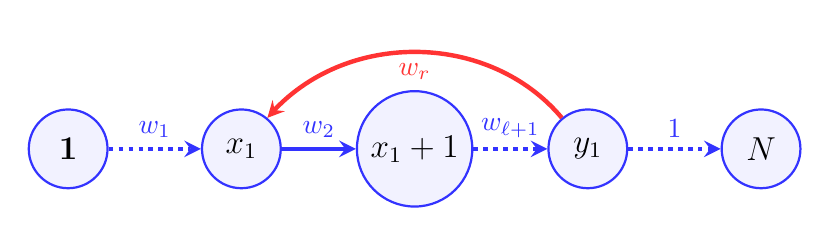
\begin{tikzpicture}[node distance=2.2cm, state/.style={circle, draw=blue!80, fill=blue!5, thick, minimum size=1.0cm, font=\large\bfseries}]
		\node[state] (1) {1};
		\node[state] (2) [right of=1] {$x_1$};
		\node[state] (3) [right of=2] {$x_1+1$};
		\node[state] (4) [right of=3] {$y_1$};
		\node[state] (5) [right of=4] {$N$};
		
		\path [->, >=stealth, ultra thick, blue!80] (1) edge[dotted] node[above] {$w_1$} (2);
		\path [->, >=stealth, ultra thick, blue!80] (2) edge node[above] {$w_2$} (3);
		\path [->, >=stealth, ultra thick, blue!80] (3) edge[dotted] node[above] {$w_{\ell+1}$} (4);
		\path [->, >=stealth, ultra thick, blue!80] (4) edge[dotted] node[above] {$1$} (5);
		\path [->, >=stealth, ultra thick, red!80] (4) edge[bend right=50] node[below] {$w_r$} (2);
	\end{tikzpicture}
	\caption{Edge-Scaled Network Topology, showing individual forward edge weight modifications $\{w_1, \dots, w_{\ell+1}\}$ along the feedback loop.}
	\label{fig:EdgeScaledNetwork}
\end{figure}

The sub-block matrix $\mathcal{C} + \mathcal{L}_{\text{re}}$ in \eqref{eq:ch_GC_OriginalLaplacian} takes the weighted form:
\begin{equation}\label{eq:ch_GC_ESChainLoop}
	\mathcal{C} + \mathcal{L}_{\text{re}} = \begin{bmatrix}
		w_1 + w_r  & 0 & \dots & 0 & -w_r \\
		-w_2 & w_2 & \dots & 0 & 0 \\
		0 & -w_3 & \dots & 0 & 0 \\
		\vdots & \vdots & \ddots & \vdots & \vdots \\
		0 & 0 & \dots & -w_{\ell+1} & w_{\ell+1}
	\end{bmatrix}
\end{equation}

Applying Gershgorin's Theorem to the columns of \eqref{eq:ch_GC_ESChainLoop}, disc 1 is centered at $w_1 + w_r$ with radius $w_2$, discs $k \in \{2, \dots, \ell\}$ are centered at $w_k$ with radii $w_{k+1}$, and disc $\ell+1$ is centered at $w_{\ell+1}$ with radius $w_r$. Ensuring all discs lie in $\mathfrak{Re}(z) > 0$ requires:
\begin{equation}\label{eq:ch_GC_ESInequality}
	w_1 + w_r > w_2 > w_3 > \dots > w_{\ell+1} > w_r
\end{equation}

By Proposition \ref{prop:ch_GC_AP_optimization}, creating an AP between $w_1 + w_r$ and $w_r$ maximizes the minimum separation $d = \frac{(w_1 + w_r) - w_r}{\ell + 1} = \frac{w_1}{\ell + 1}$. Setting $d = \frac{w_1}{\ell + 1} \ge \frac{1}{\gamma^2} \implies w_1 \ge \frac{\ell+1}{\gamma^2}$ which yields the following edge-scaling theorem:

\begin{theo}[Edge-Based Scaling for Consensus Guarantee]\label{theo2}
Consider an $N$-node directed chain of double integrators operating under protocol \eqref{eq:ch_GC_control_law} with fixed coupling $\gamma > 0$. Suppose a reverse edge of weight $w_r > 0$ is added from $y_1$ to $x_1$ ($x_1 > 1$, range $\ell$). Second-order consensus is guaranteed if forward edge weights $\{w_1, w_2, \dots, w_{\ell+1}\}$ are tuned as:
\begin{equation}\label{eq:ch_GC_ESScalar_formula}
	w_1 = \frac{\ell+1}{\gamma^2} + \epsilon, \quad w_k = w_1 + (k-1) \frac{w_1}{\ell+1}, \quad \text{for any } \epsilon > 0, k \in \{2, \dots, \ell+1\}
\end{equation}
\end{theo}

\begin{remark}[Asymmetric Sensitivity of Edge Weight Tuning]\label{rem:ch_GC_EdgeChoice}
Equation \eqref{eq:ch_GC_ESScalar_formula} demonstrates that the common difference $d = w_1 / (\ell+1)$ depends strictly on $w_1$ (the forward edge weight entering head node $x_1$ from exterior node $x_1 - 1$) and is completely independent of the reverse edge weight $w_r$. Increasing $w_1$ strengthens the authority of the upstream leader sub-chain over the loop, whereas increasing $w_r$ strengthens internal cycle feedback, degrading stability.
\end{remark}

\subsection{Combined Node-Edge Scaling Strategy}\label{sec:combo}

Combined Scaling merges node scaling factors $P = \text{diag}(p_1, \dots, p_{\ell+1})$ with edge weights $\{w_1, \dots, w_{\ell+1}\}$ to form $\tilde{P} = P(\mathcal{C} + \mathcal{L}_{\text{re}})$:
\begin{equation}\label{eq:ch_GC_eqcombined}
	\tilde{P} = \begin{bmatrix}
		p_1(w_1 + w_r)  & 0 & \dots & -p_1 w_r \\
		-p_2 w_2 & p_2 w_2 & \dots & 0 \\
		\vdots & \vdots & \ddots & \vdots \\
		0 & 0 & \dots & p_{\ell+1} w_{\ell+1}
	\end{bmatrix}
\end{equation}

Constructing an AP between $p_1(w_1 + w_r)$ and $p_1 w_r$ leads to a common difference of $d = \frac{p_1(w_1 + w_r) - p_1 w_r}{\ell + 1} = \frac{p_1 w_1}{\ell + 1}$. Setting $d \ge \frac{1}{\gamma^2} \implies p_1 w_1 \ge \frac{\ell+1}{\gamma^2}$ which yields the following result:

\begin{theo}[Combined Scaling for Consensus Guarantee]\label{theo3}
\leavevmode\par\noindent
Second-order consensus is guaranteed under protocol \eqref{eq:ch_GC_control_law} with fixed coupling $\gamma > 0$ if node factors $p_i$ and edge weights $w_i$ are selected such that:
\begin{equation}
	p_1 w_1 = \frac{\ell+1}{\gamma^2} + \epsilon, \quad p_i w_i = p_1 w_1 + (i-1) \frac{p_1 w_1}{\ell+1}, \quad \text{for } \epsilon > 0, i \in \{2, \dots, \ell+1\}
\end{equation}
\end{theo}

\begin{remark}[Implementation Flexibility of Combined Scaling]\label{rem:ch_GC_combined_flexibility}
Combined Scaling allows hardware trade-offs between node gain amplification ($p_1$) and physical edge weight adjustments ($w_1$). In physical deployments, setting $p_i = p_1$ uniformly across all cycle nodes allows edge weights $w_i$ to be adjusted within the practical bounded hardware range $w_i \in [1, 2]$.
\end{remark}


\section{Root-Locus Design Method for Loops involving the Root-Node ($x_1 = 1$)}\label{sec:ch_GC_RootLocusMethod}

When the reverse edge terminates at Node 1 itself ($x_1 = 1$, Figure \ref{fig:LeaderCycleNetwork}), Node 1 loses its zero in-degree property ($d_{\text{in}, 1} = w_r > 0$). Matrix $\mathcal{C} + \mathcal{L}_{\text{re}}$ in \eqref{eq:ch_GC_OriginalLaplacianleader} becomes a circulant-like matrix containing the zero eigenvalue $\lambda_1 = 0$. 

Under Gershgorin analysis, the column centers satisfy $2p_1, p_2, \dots, p_{\ell+1}$, but column $\ell+1$ has radius $p_1$, forcing condition $p_1 > p_2 > \dots > p_{\ell+1} > p_1$, which is impossible to satisfy. Thus, Gershgorin-based disc separation fails entirely for root-node loops.

To resolve this structural singularity, we formulate a complementary root-locus control framework.

\subsection{Complementary Root-Locus Formulation}

Suppose the control dynamics of all nodes in the root loop $\{1, 2, \dots, y_1\}$ are scaled by node factor $\alpha > 0$. Additionally, let the forward edge weight connecting Node 1 to Node 2 be scaled by edge factor $\beta / \alpha > 0$, where $\alpha$ and $\beta$ are design parameters. The loop sub-block matrix $\mathcal{C} + \mathcal{L}_{\text{re}} \in \mathbb{R}^{(\ell+1) \times (\ell+1)}$ takes the form:
\begin{equation}\label{eq:ch_GC_scaledmatrix}
	\mathcal{C} + \mathcal{L}_{\text{re}} = \begin{bmatrix}
		\alpha  & 0 & 0 & \dots & -\alpha \\
		-\beta & \beta & 0 & \dots & 0 \\
		0 & -\alpha & \alpha & \dots & 0 \\
		\vdots & \vdots & \ddots & \ddots & \vdots \\
		0 & 0 & \dots & -\alpha & \alpha
	\end{bmatrix}
\end{equation}

Computing the characteristic polynomial of \eqref{eq:ch_GC_scaledmatrix}:
\begin{equation}\label{eq:ch_GC_chareq}
	(s - \alpha)^\ell (s - \beta) + (-1)^\ell \alpha^\ell \beta = 0
\end{equation}
Rearranging \eqref{eq:ch_GC_chareq} into standard $1 + K G(s) = 0$ feedback form:
\begin{equation}\label{eq:ch_GC_rearrangedchar}
	1 + \beta \cdot G(s) = 0, \quad \text{where } G(s) \coloneqq \frac{(s - \alpha)^\ell - (-\alpha)^\ell}{s (s - \alpha)^\ell}
\end{equation}

\begin{figure}[ht!]
	\centering
	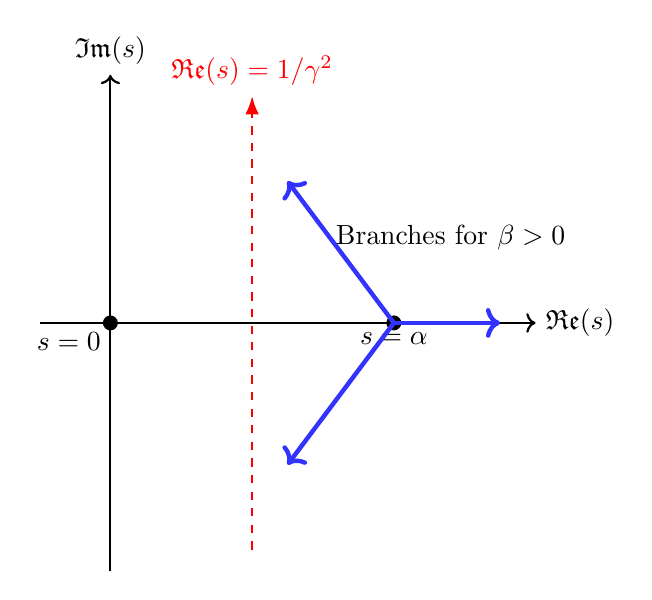
\begin{tikzpicture}[scale=0.9]
		\draw[->, thick] (-1,0) -- (6,0) node[right] {$\mathfrak{Re}(s)$};
		\draw[->, thick] (0,-3.5) -- (0,3.5) node[above] {$\mathfrak{Im}(s)$};
		
		\fill (0,0) circle (3pt) node[below left] {$s=0$};
		\fill (4,0) circle (3pt) node[below] {$s=\alpha$};
		
		\draw[dashed, red, thick] (2, -3.2) -- (2, 3.2) node[above] {$\mathfrak{Re}(s) = 1/\gamma^2$};
		
		\draw[ultra thick, blue!80, ->] (4,0) -- (2.5, 2.0);
		\draw[ultra thick, blue!80, ->] (4,0) -- (2.5, -2.0);
		\draw[ultra thick, blue!80, ->] (4,0) -- (5.5, 0);
		
		\node at (4.8, 1.2) {Branches for $\beta > 0$};
	\end{tikzpicture}
	\caption{Complementary Root-Locus trajectory of $G(s)$ for fixed $\alpha > 1/\gamma^2$ as gain $\beta$ increases from 0. Branches emanate from pole $s = \alpha$ toward the imaginary axis.}
	\label{fig:RootLocusBasedNetwork}
\end{figure}

The open-loop poles of $G(s)$ reside at $s = 0$ (simple) and $s = \alpha$ (multiplicity $\ell$). The open-loop zeros reside at $s = \alpha \left( 1 + e^{j \frac{\pi}{\ell}(2k+1)} \right)$ for odd $\ell$, and $s = \alpha \left( 1 + e^{j \frac{\pi}{\ell}(2k)} \right)$ for even $\ell$. Note that $G(s)$ possesses a pole-zero cancellation at the origin $s = 0$.

For $\beta = 0$, all non-zero roots reside at $s = \alpha$. As gain $\beta > 0$ increases, root locus branches emanate from $s = \alpha$ and head toward the imaginary axis (Figure \ref{fig:RootLocusBasedNetwork}). To preserve consensus under fixed coupling $\gamma$, we select $\alpha > 1/\gamma^2$ and bound gain $\beta$ such that no root branch crosses to the left of $\mathfrak{Re}(z) = 1/\gamma^2$:

\begin{theo}[Root-Locus based Gain Scaling for Consensus Guarantee]\label{theo3ES}
\leavevmode\par\noindent
Consider an $N$-node directed chain of double integrators operating under protocol \eqref{eq:ch_GC_control_law} with fixed coupling $\gamma > 0$. Suppose a reverse edge is added from $y_1$ to $x_1 = 1$ ($x_1 = 1$, range $\ell$). Select node scaling factor $\alpha > 1/\gamma^2$. Then, there exists a upper gain bound $\bar{\beta} > 0$ such that when the control law of one agent in the loop is scaled by $\beta / \alpha$ (with $0 < \beta < \bar{\beta}$), second-order consensus is guaranteed.
\end{theo}

\begin{proof}
For $\beta = 0$, the non-zero roots of \eqref{eq:ch_GC_chareq} reside at $s = \alpha > 1/\gamma^2$, satisfying condition \eqref{eq:ch_GC_dubey_bound}. By root continuity with respect to parameter variations, for any $\alpha > 1/\gamma^2$, there exists $\bar{\beta} > 0$ such that for all $0 < \beta < \bar{\beta}$, all non-zero roots satisfy $\mathfrak{Re}(s_i) \ge 1/\gamma^2$, guaranteeing consensus.
\end{proof}

\subsection{Single-Gain Cyclic Pursuit Synthesis (One Cycle, One Gain)}

To prevent edge-weakening ($\beta \to 0$) when root-node forms a part of the loop, we synthesize an equal-weight cyclic pursuit design where all edges in the cycle share an identical weight $\alpha > 0$.

\begin{theo}[Single-Gain Threshold for Root-Node Loops]\label{theoonegain}
\leavevmode\par\noindent
Consider an $N$-agent double-integrator network containing a root-node loop of range $\ell$ with equal edge weights $\alpha > 0$. Second-order consensus is guaranteed under fixed coupling parameter $\gamma > 0$ if $\alpha$ satisfies:
\begin{equation}\label{eq:ch_GC_onegain_bound}
	\alpha \ge \frac{\cot^2\left(\frac{\pi}{\ell+1}\right)}{2\gamma^2}
\end{equation}
\end{theo}

\begin{proof}
For an $(\ell+1)$-node cyclic pursuit graph with equal edge weights $\alpha$, the characteristic equation is $(s + \alpha)^{\ell+1} = \alpha^{\ell+1}$. The roots are:
\begin{equation}\label{eq:ch_GC_rootsunity}
	s_k = \alpha \left( e^{j \frac{2\pi k}{\ell+1}} - 1 \right), \quad k \in \{0, 1, \dots, \ell\}
\end{equation}
The non-zero eigenvalues of the Laplacian $\mathcal{L}_{\text{root}}$ are $\lambda_k = -s_k = \alpha \left( 1 - e^{j \frac{2\pi k}{\ell+1}} \right)$. All non-zero eigenvalues lie on a circle of radius $\alpha$ centered at $(\alpha, 0)$ in the complex plane, tangent to the imaginary axis at the origin (Figure \ref{fig:SineAngle}).

\begin{figure}[ht!]
	\centering
	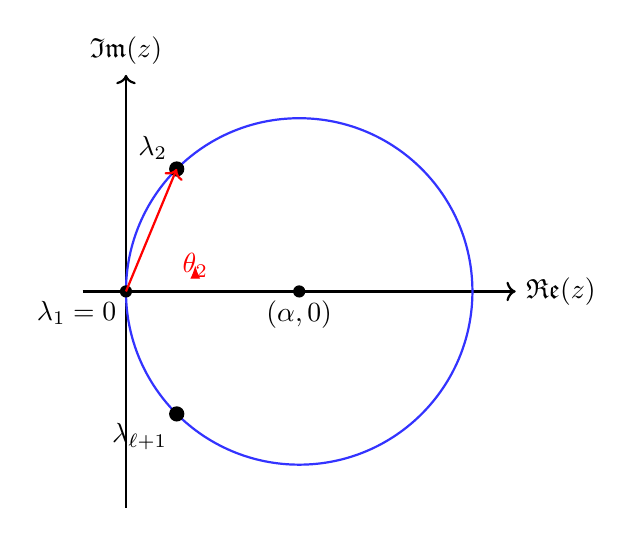
\begin{tikzpicture}[scale=1.1]
		\draw[->, thick] (-0.5,0) -- (4.5,0) node[right] {$\mathfrak{Re}(z)$};
		\draw[->, thick] (0,-2.5) -- (0,2.5) node[above] {$\mathfrak{Im}(z)$};
		\draw[thick, blue!80] (2,0) circle (2cm);
		\fill (2,0) circle (2pt) node[below] {$(\alpha,0)$};
		\fill (0,0) circle (2pt) node[below left] {$\lambda_1=0$};
		
		\fill (0.586, 1.414) circle (2.5pt) node[above left] {$\lambda_2$};
		\fill (0.586, -1.414) circle (2.5pt) node[below left] {$\lambda_{\ell+1}$};
		\draw[thick, red, ->] (0,0) -- (0.586, 1.414);
		\draw[red] (0.8, 0.3) node {$\theta_2$};
	\end{tikzpicture}
	\caption{Eigenvalue distribution of an $(\ell+1)$-node equal-weight cyclic pursuit Laplacian on a circle of radius $\alpha$. Eigenvalue $\lambda_2$ (corresponding to $k=1$) subtends the maximum ray angle $\theta_2$.}
	\label{fig:SineAngle}
\end{figure}

The necessary and sufficient consensus condition \eqref{eq:ch_GC_yu_threshold_recap} can be re-written in polar form as $\gamma \ge \max_k \frac{\sin \theta_k}{\sqrt{\mathfrak{Re}(\lambda_k)}}$, where $\theta_k$ is the ray angle subtended by $\lambda_k$ at the origin. By Proposition \ref{prop:ch_GC_chord_geometry}, the eigenvalue closest to the origin ($\lambda_2$, corresponding to $k=1$) subtends the maximum ray angle $\theta_2 = \frac{\pi}{2} - \frac{\pi}{\ell+1}$. 

Computing $\mathfrak{Re}(\lambda_2) = \alpha \left( 1 - \cos\left(\frac{2\pi}{\ell+1}\right) \right) = 2\alpha \sin^2\left(\frac{\pi}{\ell+1}\right)$ and $\sin(\theta_2) = \cos\left(\frac{\pi}{\ell+1}\right)$:
\begin{equation}
	\frac{\sin \theta_2}{\sqrt{\mathfrak{Re}(\lambda_2)}} = \frac{\cos\left(\frac{\pi}{\ell+1}\right)}{\sqrt{2\alpha \sin^2\left(\frac{\pi}{\ell+1}\right)}} = \frac{\cot\left(\frac{\pi}{\ell+1}\right)}{\sqrt{2\alpha}}
\end{equation}
Substituting this expression into $\gamma \ge \frac{\sin \theta_2}{\sqrt{\mathfrak{Re}(\lambda_2)}}$:
\begin{equation}
	\gamma \ge \frac{\cot\left(\frac{\pi}{\ell+1}\right)}{\sqrt{2\alpha}} \implies \gamma^2 \ge \frac{\cot^2\left(\frac{\pi}{\ell+1}\right)}{2\alpha} \implies \alpha \ge \frac{\cot^2\left(\frac{\pi}{\ell+1}\right)}{2\gamma^2}
\end{equation}
which completes the proof.
\end{proof}

\section{Numerical Simulations}\label{sec:ch_GC_simulations}
To demonstrate the efficacy of the proposed localized remedies, simulations were conducted on a 10-agent network ($N = 10$) governed by double-integrator dynamics with a predesigned velocity coupling parameter $\gamma = 0.5$.
A reverse edge of unit weight ($w_r = 1$) is inserted from node $y_1 = 9$ to node $x_1 = 3$, creating a feedback loop of range $\ell = y_1 - x_1 = 6$. The unperturbed nominal chain operates under Laplacian $\mathcal{L}$. With the reverse edge added, the modified sub-block $\mathcal{C} + \mathcal{L}_{\text{re}}$ (spanning nodes 3 through 9) takes the 7-dimensional form:
\begin{equation} \label{eq:ch_GC_ExampleLaplacian_block}
	\mathcal{C} + \mathcal{L}_{\text{re}} = \begin{bmatrix}
		2 & 0 & 0 & 0 & 0 & 0 & -1 \\
		-1 & 1 & 0 & 0 & 0 & 0 & 0 \\
		0 & -1 & 1 & 0 & 0 & 0 & 0 \\
		0 & 0 & -1 & 1 & 0 & 0 & 0 \\
		0 & 0 & 0 & -1 & 1 & 0 & 0 \\
		0 & 0 & 0 & 0 & -1 & 1 & 0 \\
		0 & 0 & 0 & 0 & 0 & -1 & 1
	\end{bmatrix}
\end{equation}
Under the unperturbed reverse edge, applying Yu's exact threshold \eqref{eq:ch_GC_yu_threshold_recap} reveals that the modified network requires $\gamma \ge 1.2134$. Because the predesigned global parameter is fixed at $\gamma = 0.5 < 1.2134$, consensus breaks down completely, as demonstrated by the diverging position and velocity trajectories in Figures \ref{fig:10-9-3_OriginalLaplacianGamma0.5PositionConsensus} and \ref{fig:10-9-3_OriginalLaplacianGamma0.5VelocityConsensus}. If $\gamma$ were retuned globally to $\gamma = 1.5$, consensus would be restored (Figures \ref{fig:10-9-3_OriginalLaplacianGamma1.5PositionConsensus} and \ref{fig:10-9-3_OriginalLaplacianGamma1.5VelocityConsensus}), but this requires global access to the Laplacian spectrum of the graph that results from the addition of the reverse edge.
\begin{figure}[ht!]
	\centering
	\begin{subfigure}[b]{1.0\textwidth}
		\centering
		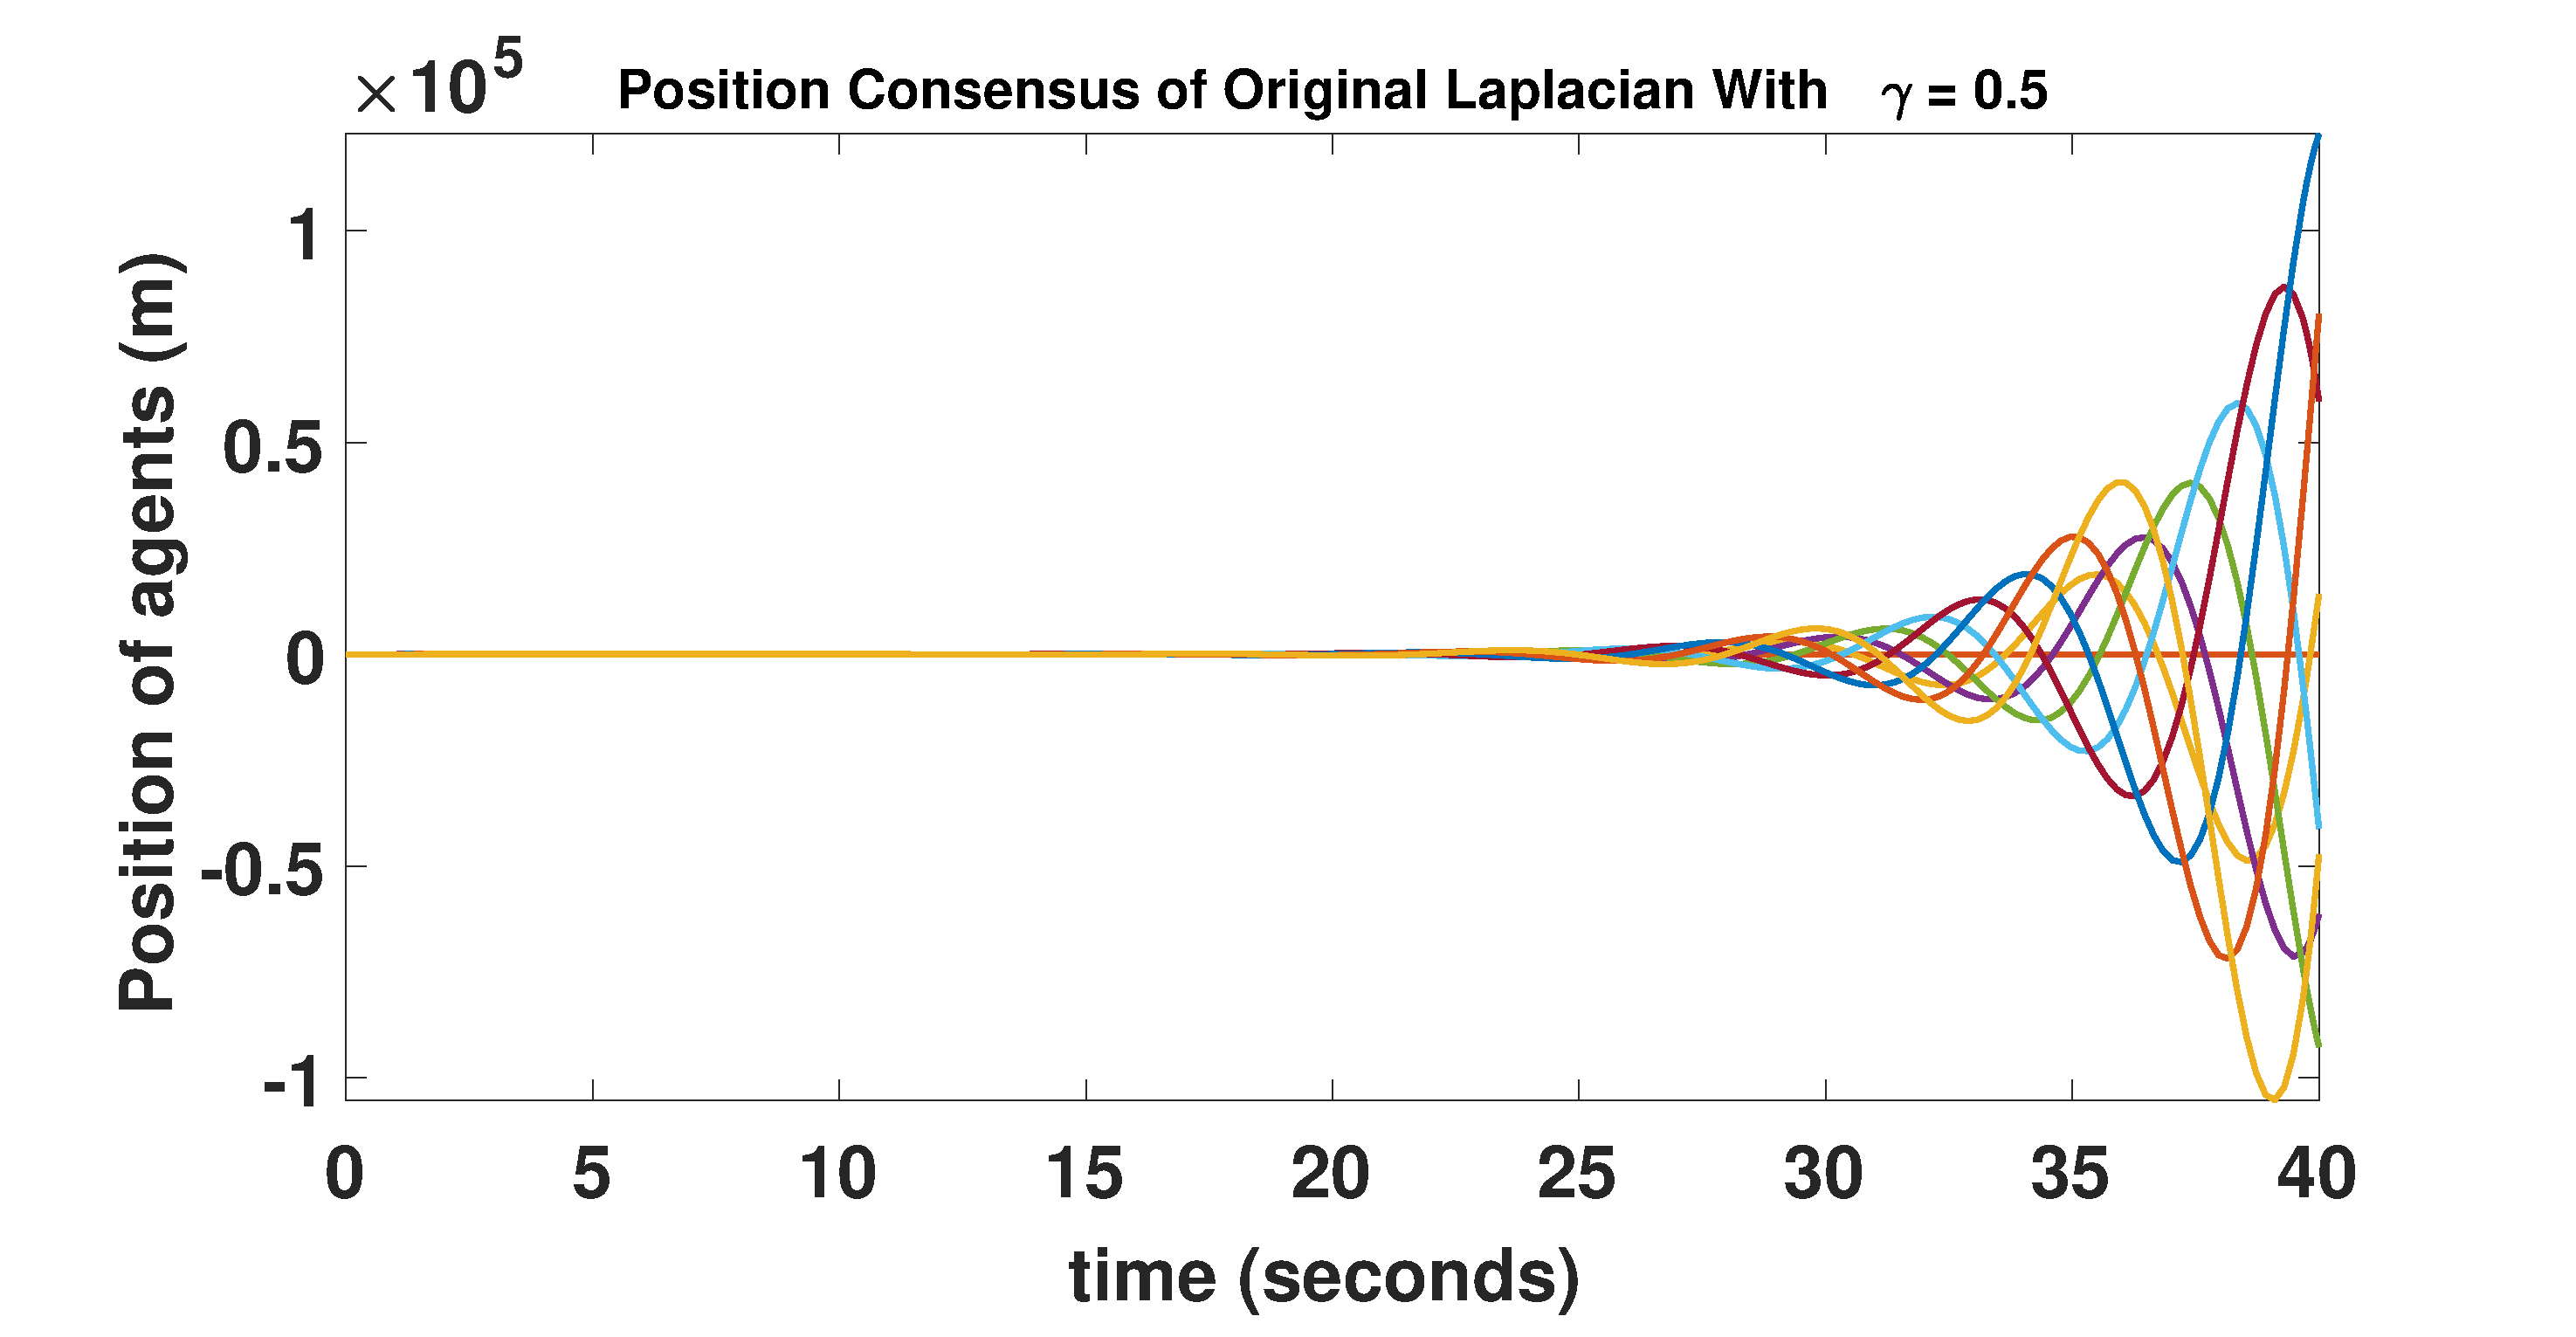
\includegraphics[width=\textwidth, keepaspectratio]{3_Images/10-9-3_OriginalLaplacianGamma0.5PositionConsensus.eps}
		\caption{Position trajectory divergence ($\gamma = 0.5$).}
		\label{fig:10-9-3_OriginalLaplacianGamma0.5PositionConsensus}
	\end{subfigure}
	
	\vspace{1em} % Adds vertical separation between stacked subfigures
	
	\begin{subfigure}[b]{1.0\textwidth}
		\centering
		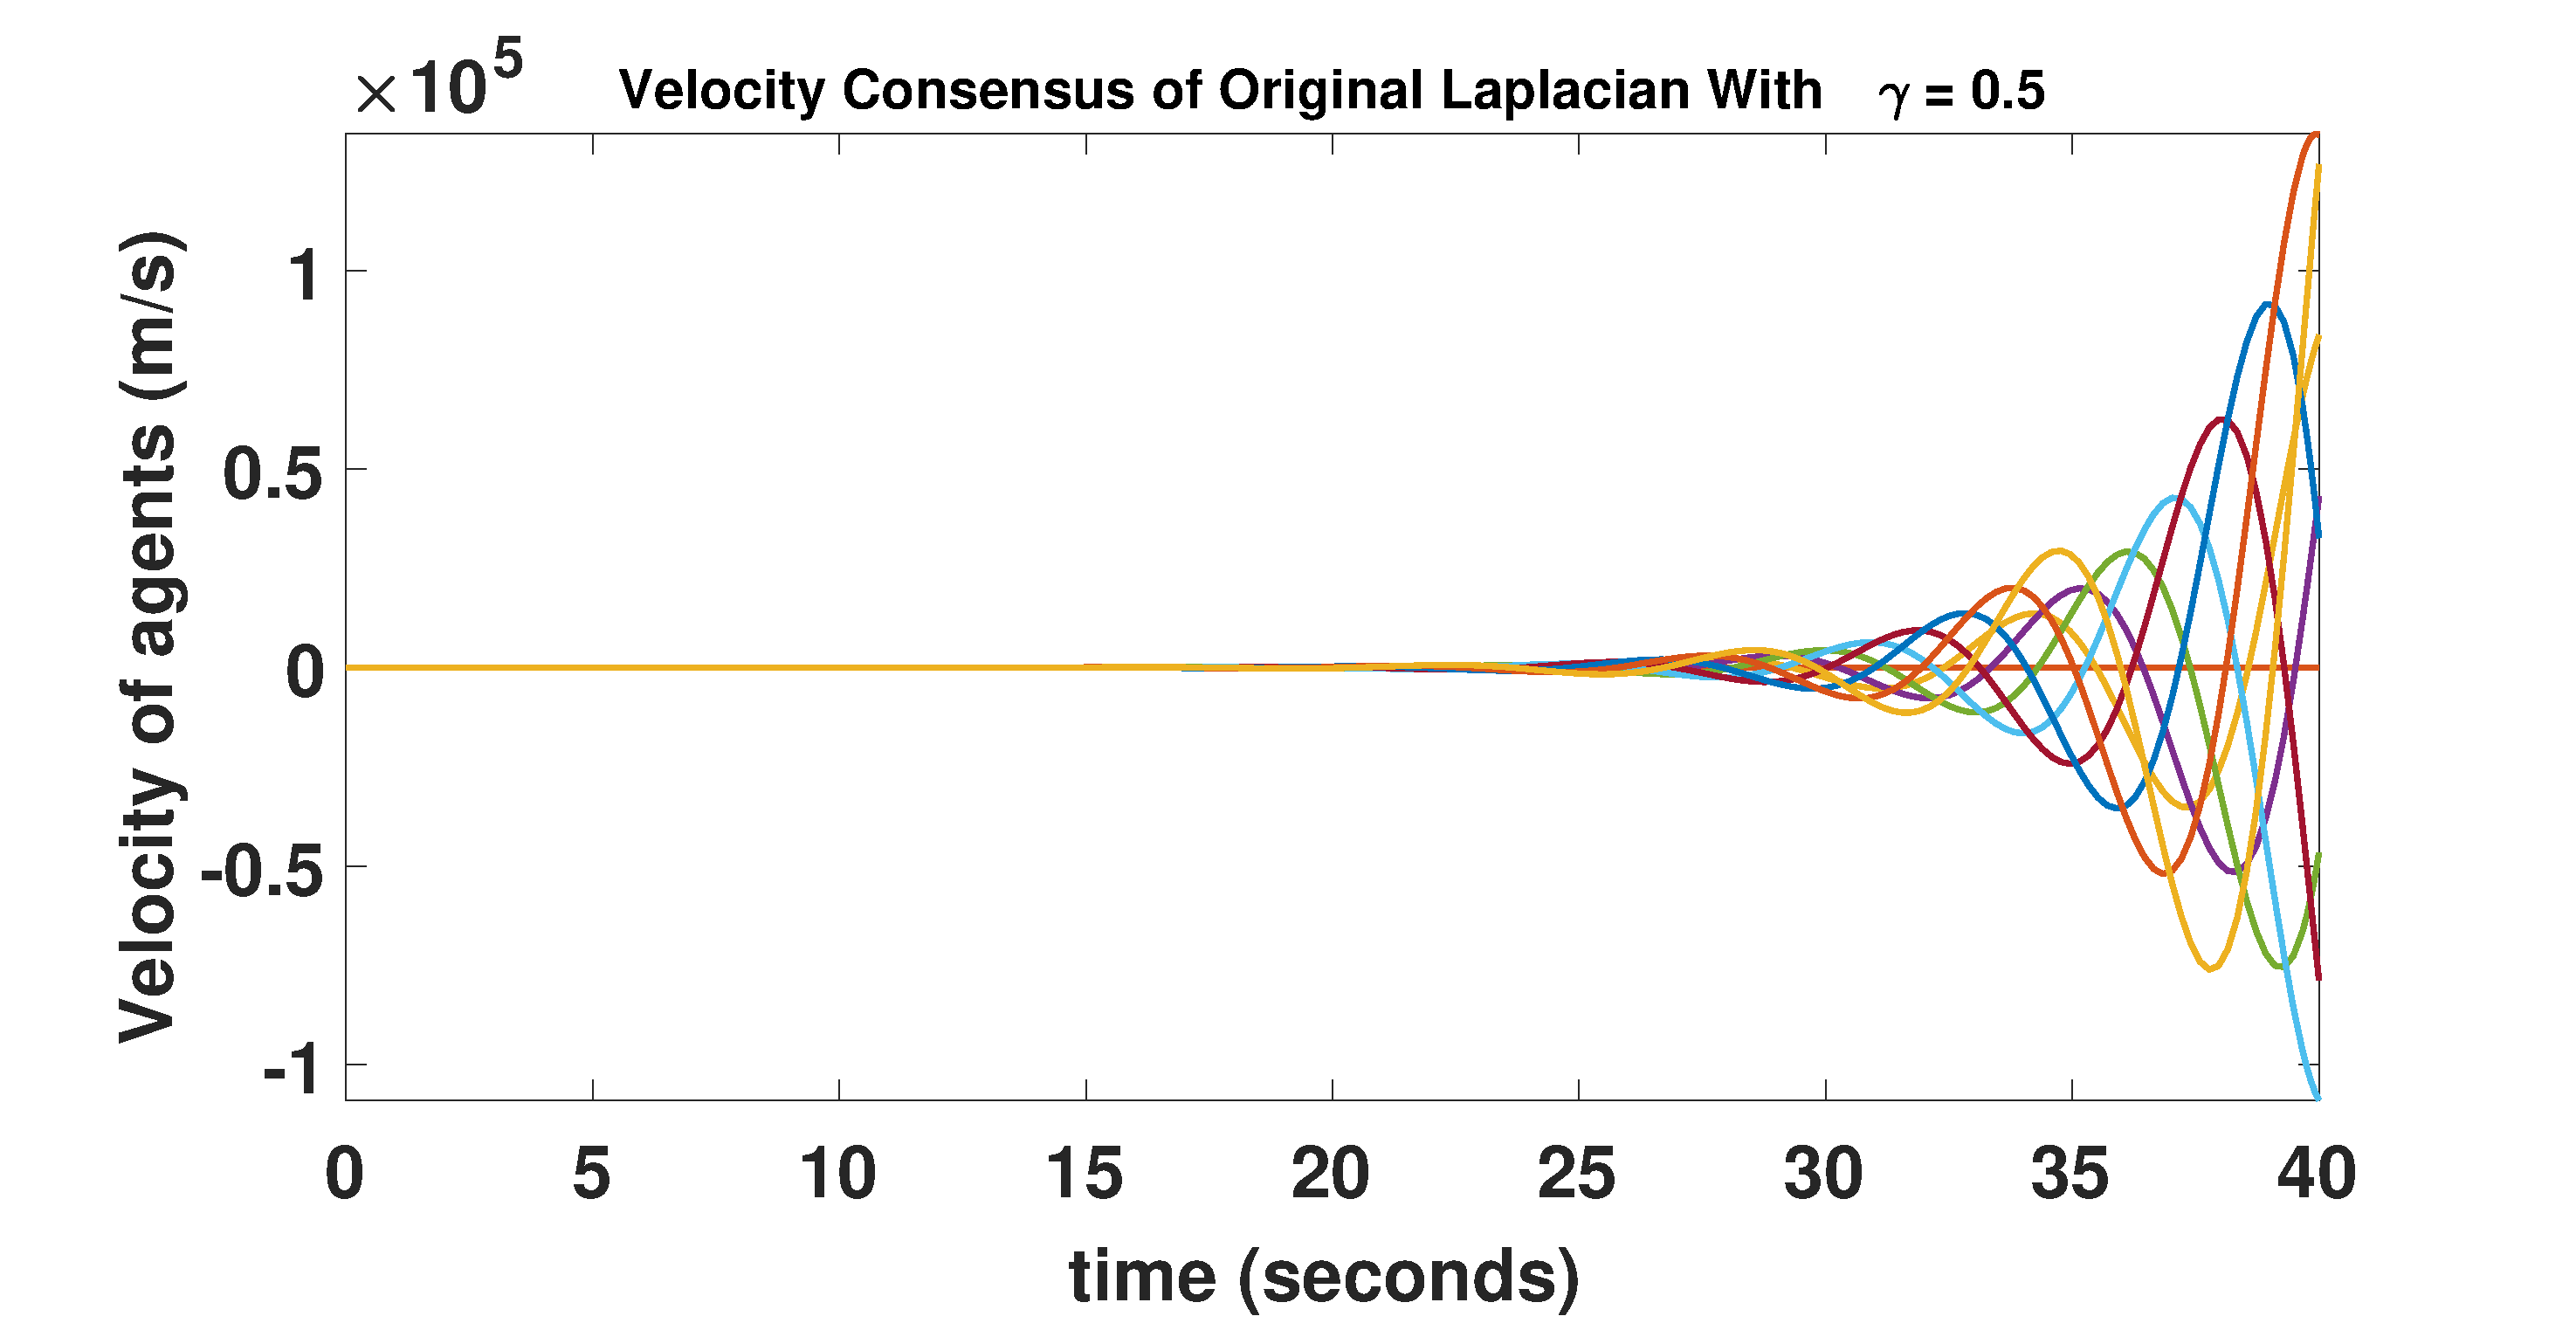
\includegraphics[width=\textwidth, keepaspectratio]{3_Images/10-9-3_OriginalLaplacianGamma0.5VelocityConsensus.eps}
		\caption{Velocity trajectory divergence ($\gamma = 0.5$).}
		\label{fig:10-9-3_OriginalLaplacianGamma0.5VelocityConsensus}
	\end{subfigure}
	\caption{Consensus breakdown in a 10-agent network under unperturbed reverse edge ($y_1=9, x_1=3, \ell=6$) when fixed coupling $\gamma = 0.5 < 1.2134$.}
	\label{fig:unperturbed_breakdown}
\end{figure}

\begin{figure}[ht!]
	\centering
	\begin{subfigure}[b]{\textwidth}
		\centering
		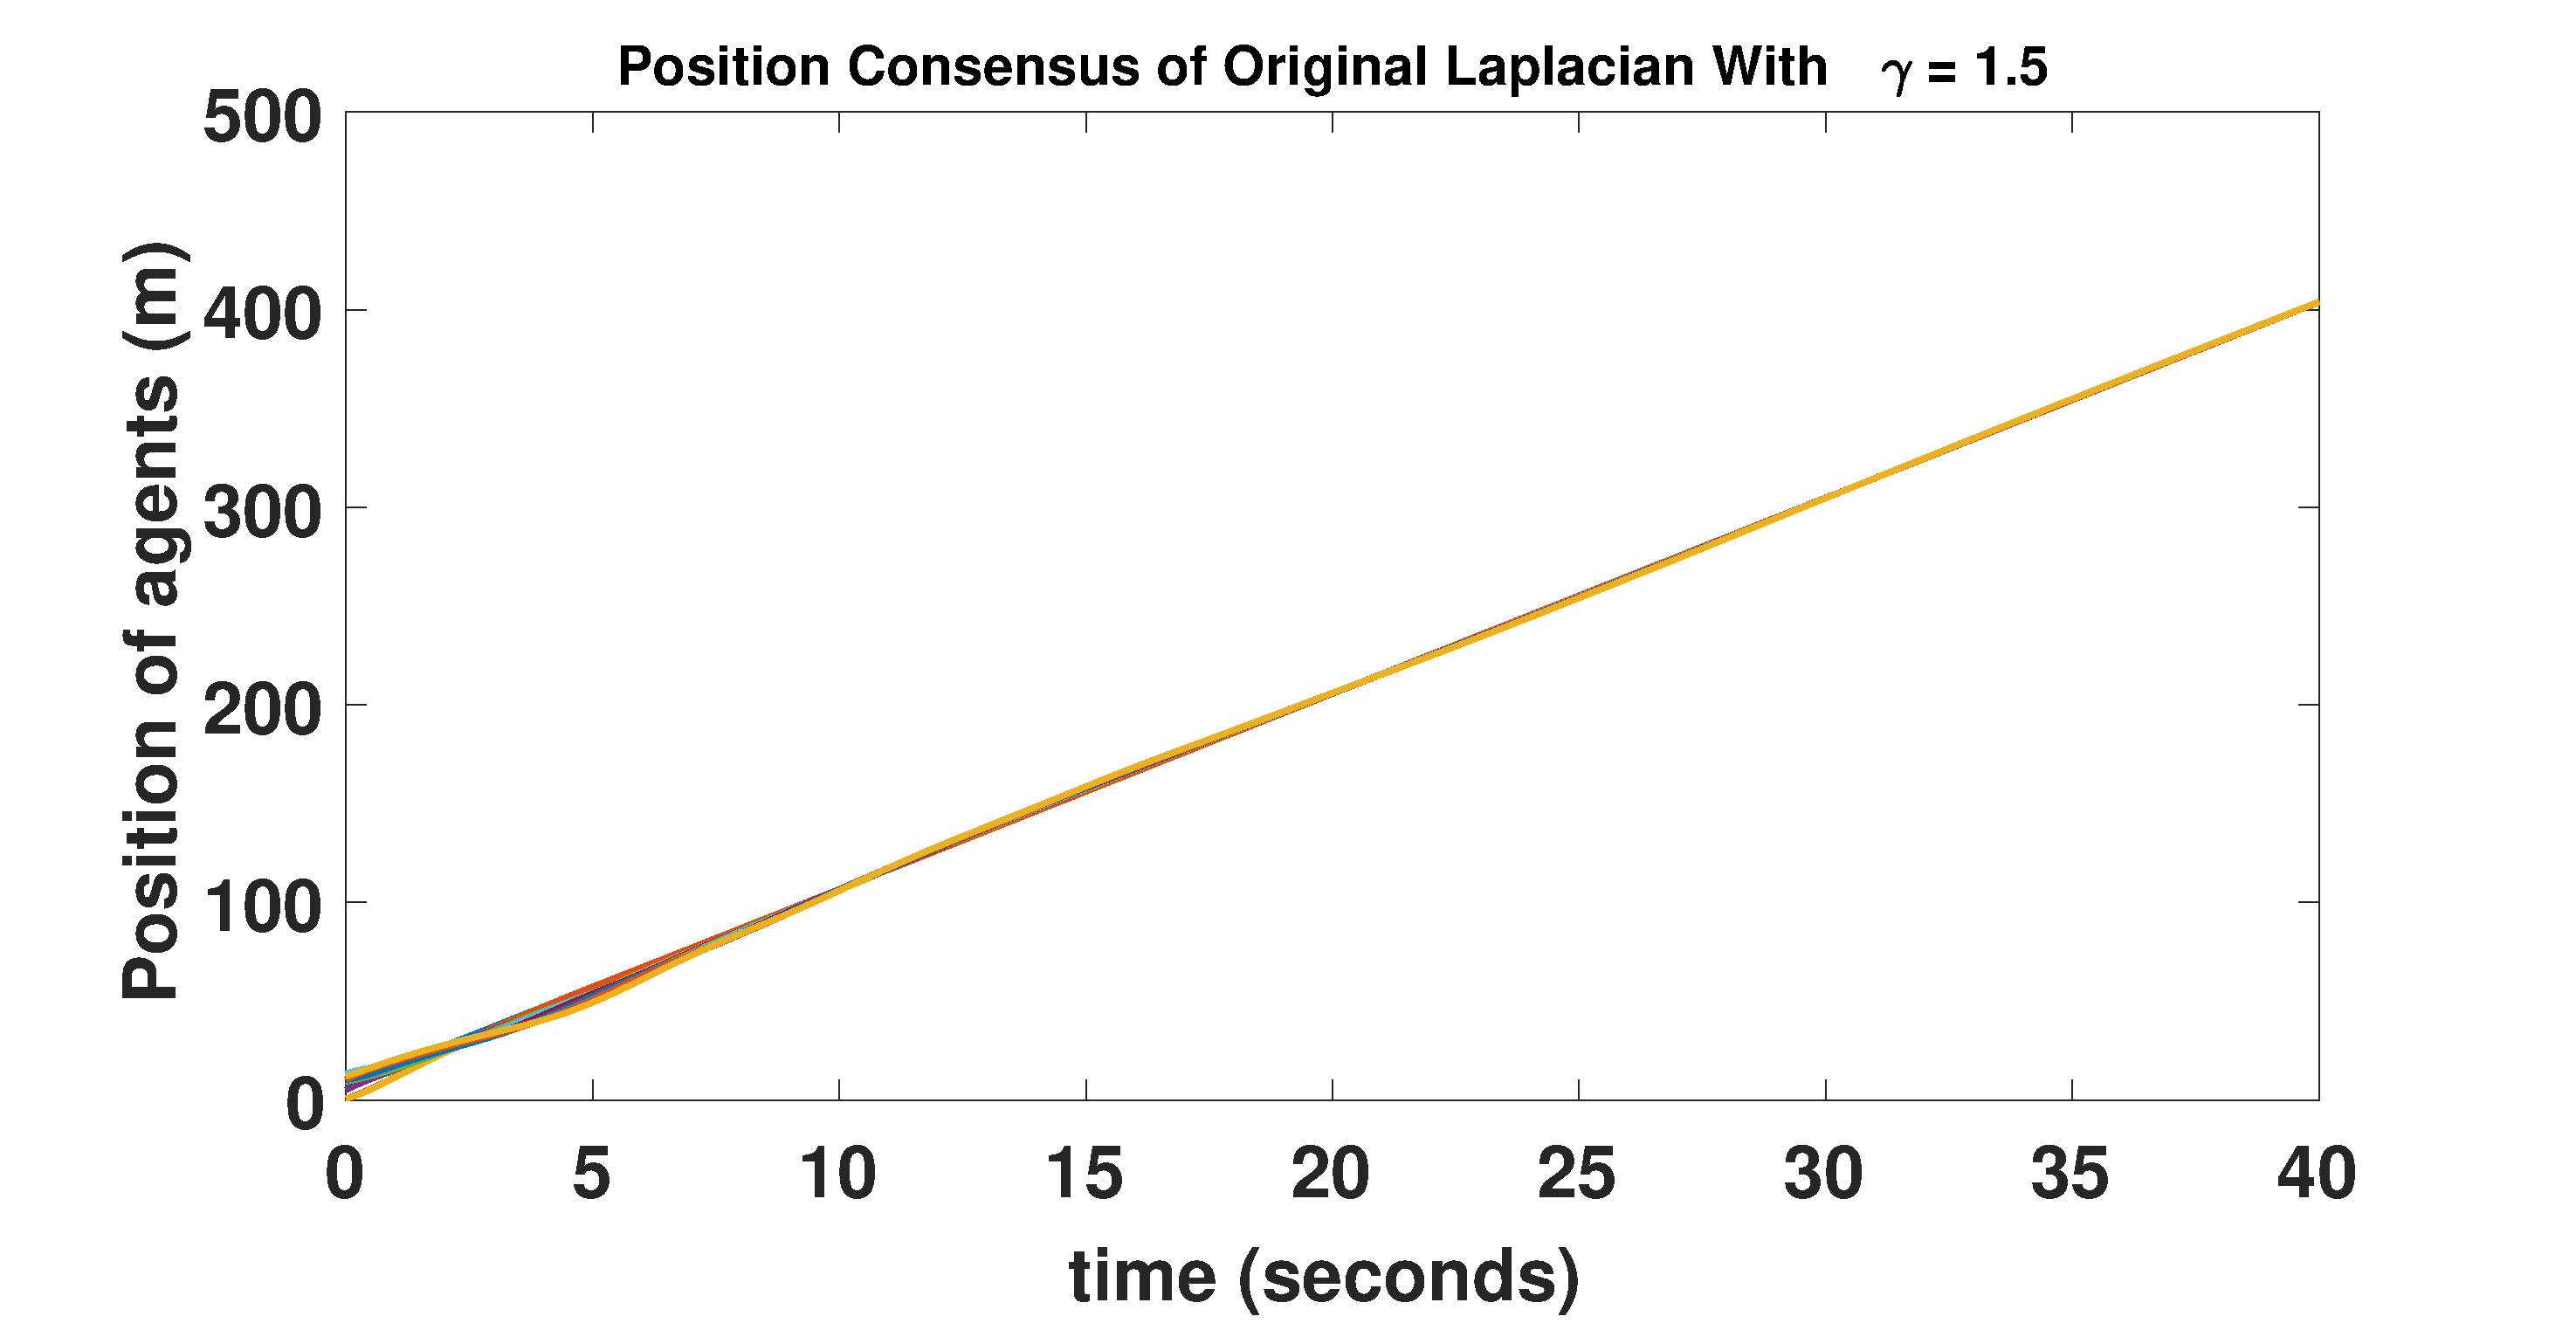
\includegraphics[width=\textwidth, keepaspectratio]{3_Images/10-9-3_OriginalLaplacianGamma1.5PositionConsensus.eps}
		\caption{Position consensus restored ($\gamma = 1.5$).}
		\label{fig:10-9-3_OriginalLaplacianGamma1.5PositionConsensus}
	\end{subfigure}
	\hfill
	\begin{subfigure}[b]{\textwidth}
		\centering
		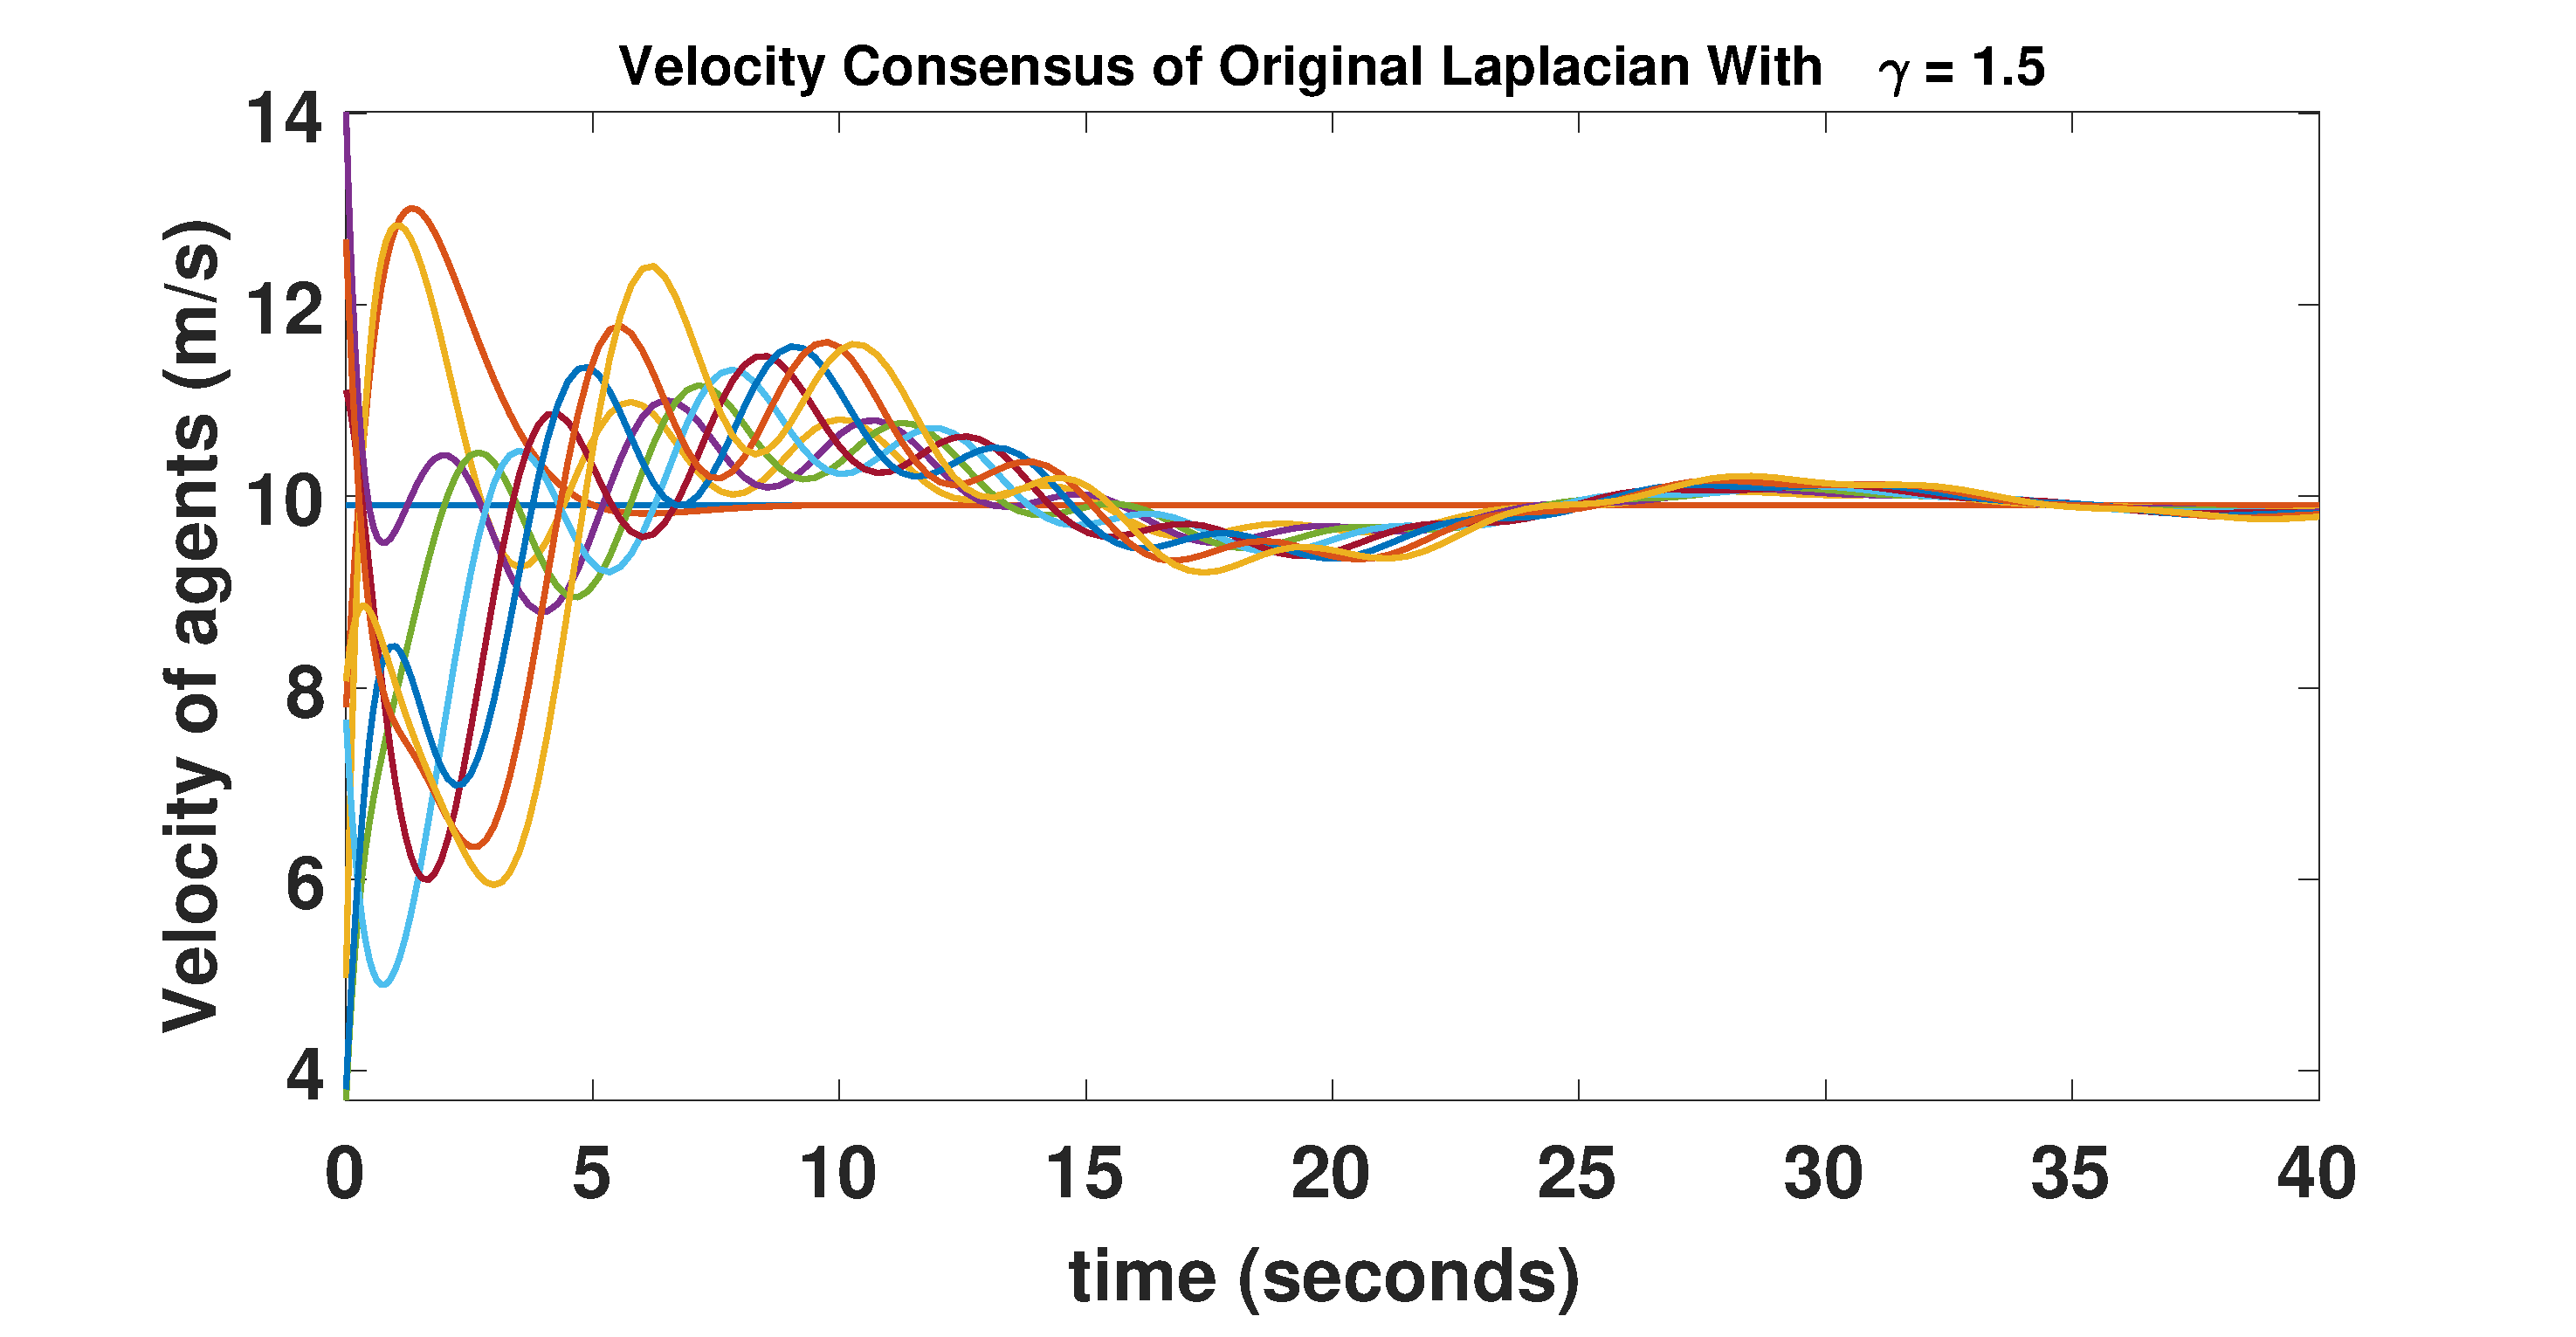
\includegraphics[width=\textwidth, keepaspectratio]{3_Images/10-9-3_OriginalLaplacianGamma1.5VelocityConsensus.eps}
		\caption{Velocity consensus restored ($\gamma = 1.5$).}
		\label{fig:10-9-3_OriginalLaplacianGamma1.5VelocityConsensus}
	\end{subfigure}
	\caption{Restoration of consensus by retuning global coupling to $\gamma = 1.5 > 1.2134$ (requires global network access).}
	\label{fig:global_retuning}
\end{figure}
\subsection{Validation of Localized Scaling Remedies ($x_1 = 3 > 1$)}
We now apply the localized scaling remedies without modifying $\gamma = 0.5$:

1. \textbf{Node-Based Scaling:} Applying Theorem \ref{theo1} with $\gamma = 0.5$ and $\ell = 6$, $p_1 \ge \frac{7}{0.25} = 28$. Selecting $p_1 = 31.5$ and creating a 7-term AP between $p_1 = 31.5$ and $2p_1 = 63$ gives common difference $d = 4.5$. The scaling matrix is $P = \text{diag}(31.5, 58.5, 54, 49.5, 45, 40.5, 36)$. Under $P$, the required coupling threshold drops to $\gamma \ge 0.1822 < 0.5$. Figures \ref{fig:10-9-3_NodeScaledLaplacianGamma0.5PositionConsensus} and \ref{fig:10-9-3_NodeScaledLaplacianGamma0.5VelocityConsensus} confirm asymptotic state agreement under $\gamma = 0.5$.

\begin{figure}[ht!]
	\centering
	\begin{subfigure}[b]{\textwidth}
		\centering
		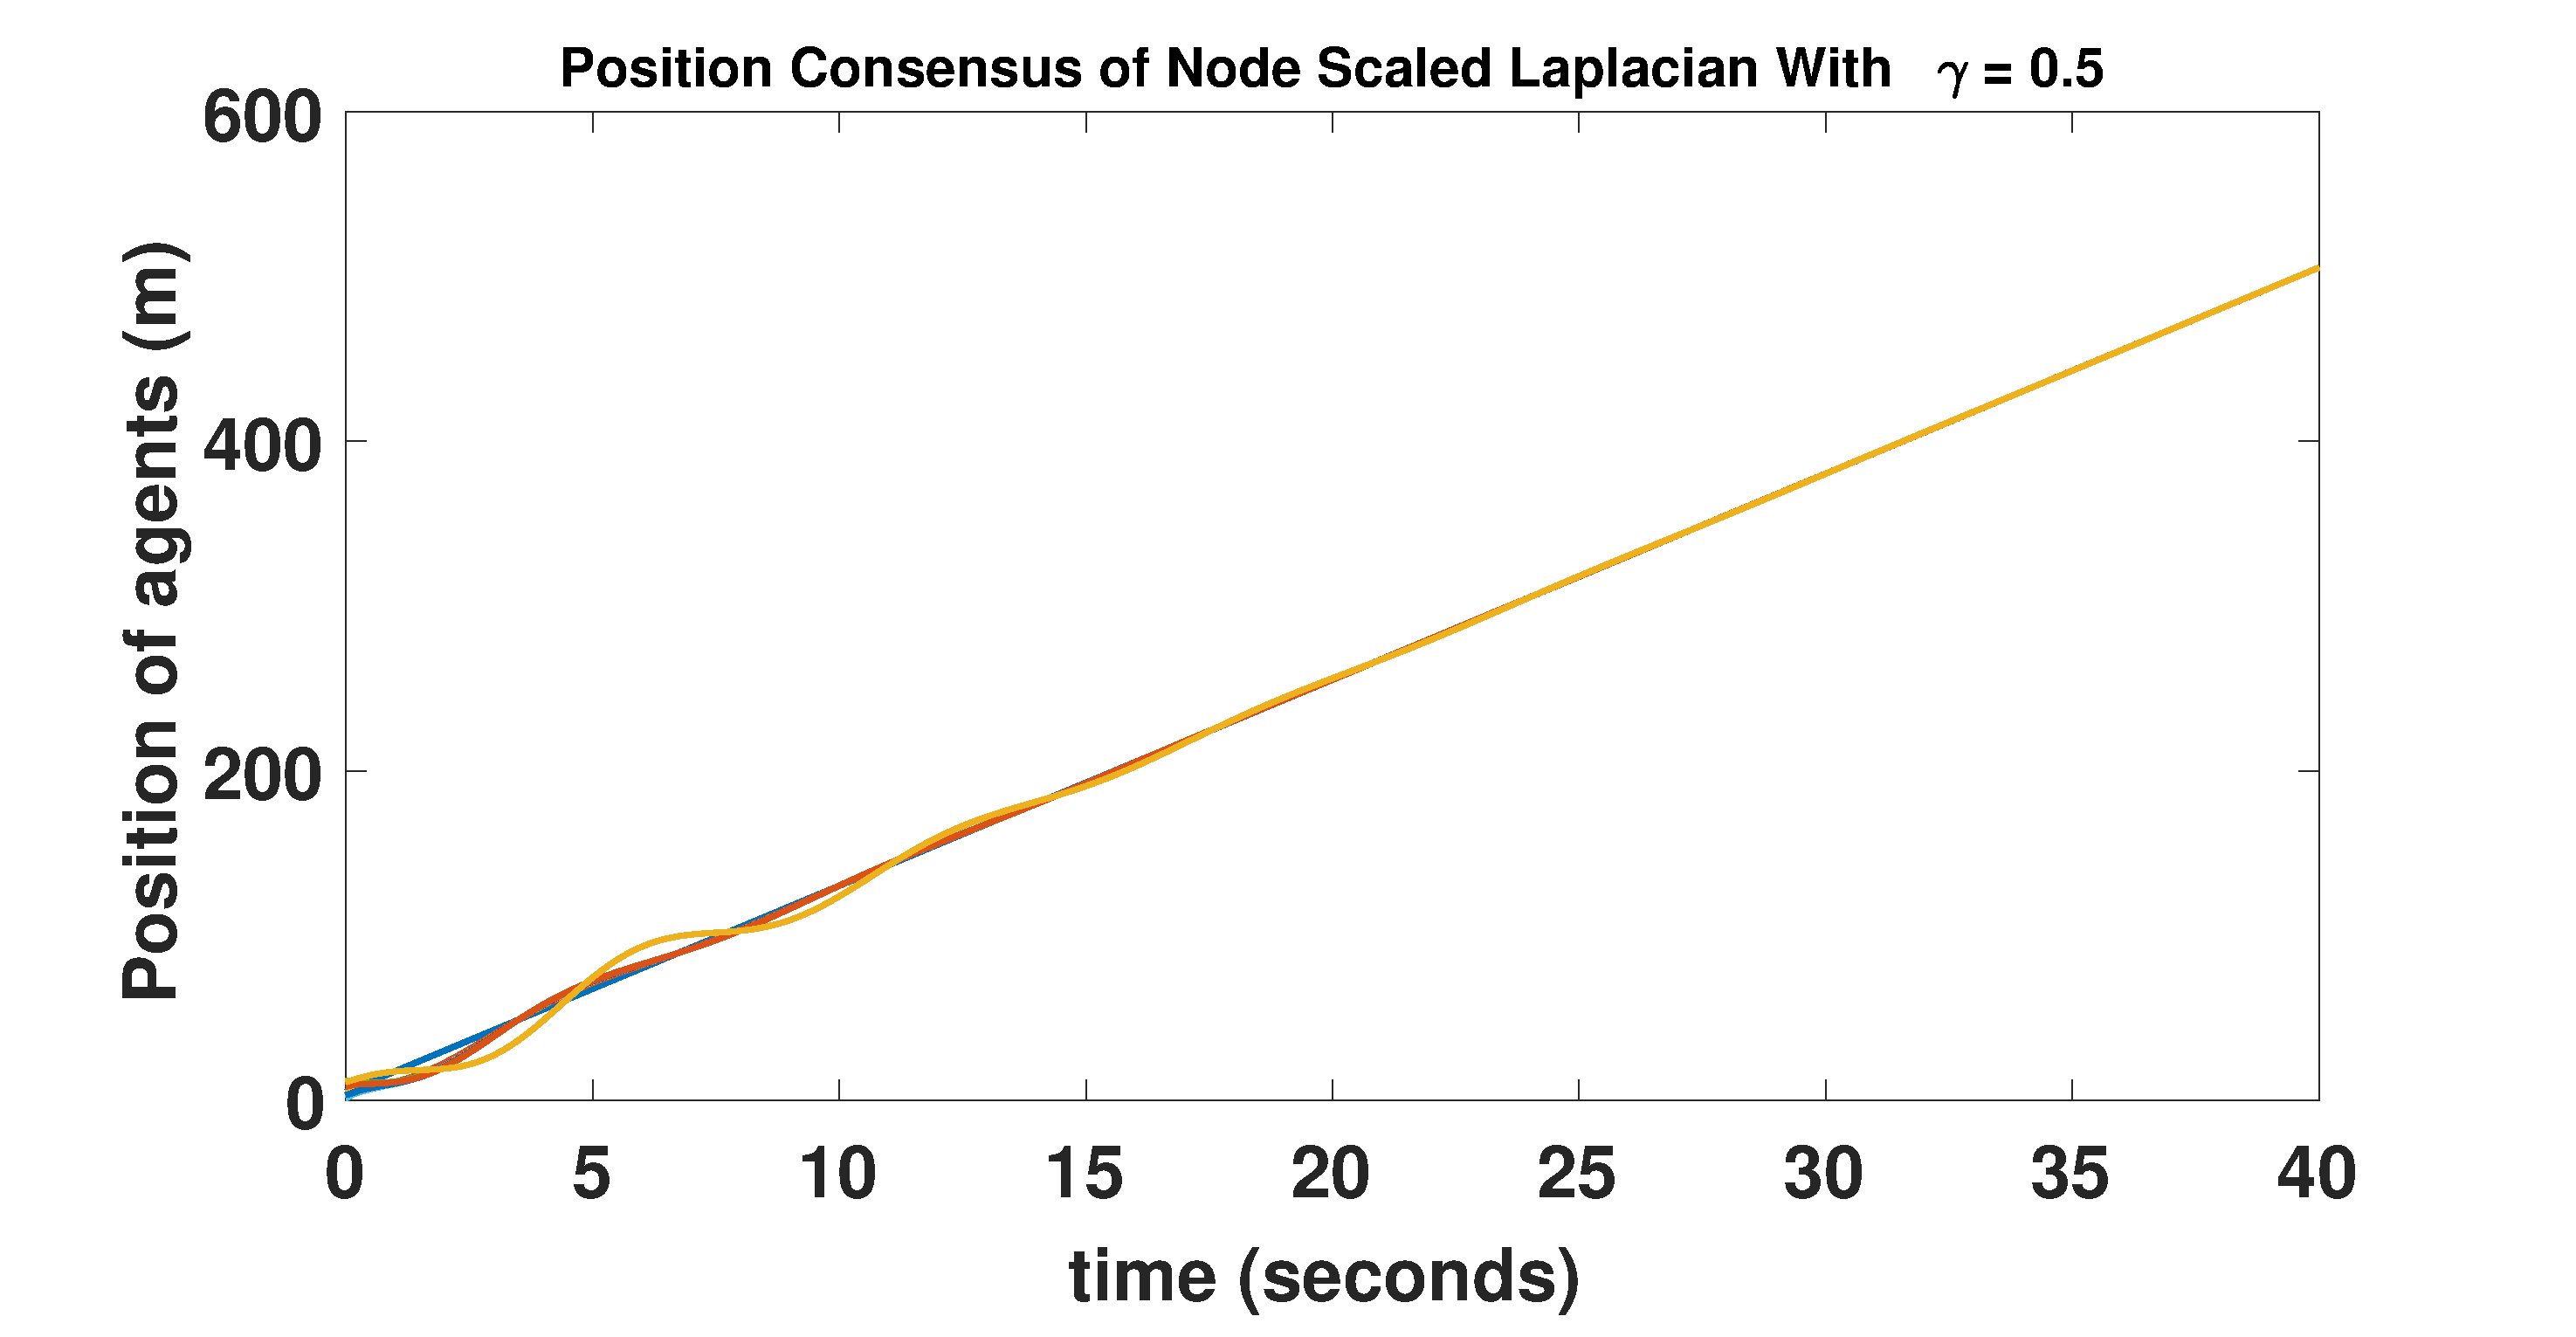
\includegraphics[width=\textwidth, keepaspectratio]{3_Images/10-9-3_NodeScaledLaplacianGamma0.5PositionConsensus.eps}
		\caption{Node-Scaled Position Consensus ($\gamma = 0.5$).}
		\label{fig:10-9-3_NodeScaledLaplacianGamma0.5PositionConsensus}
	\end{subfigure}
	\hfill
	\begin{subfigure}[b]{\textwidth}
		\centering
		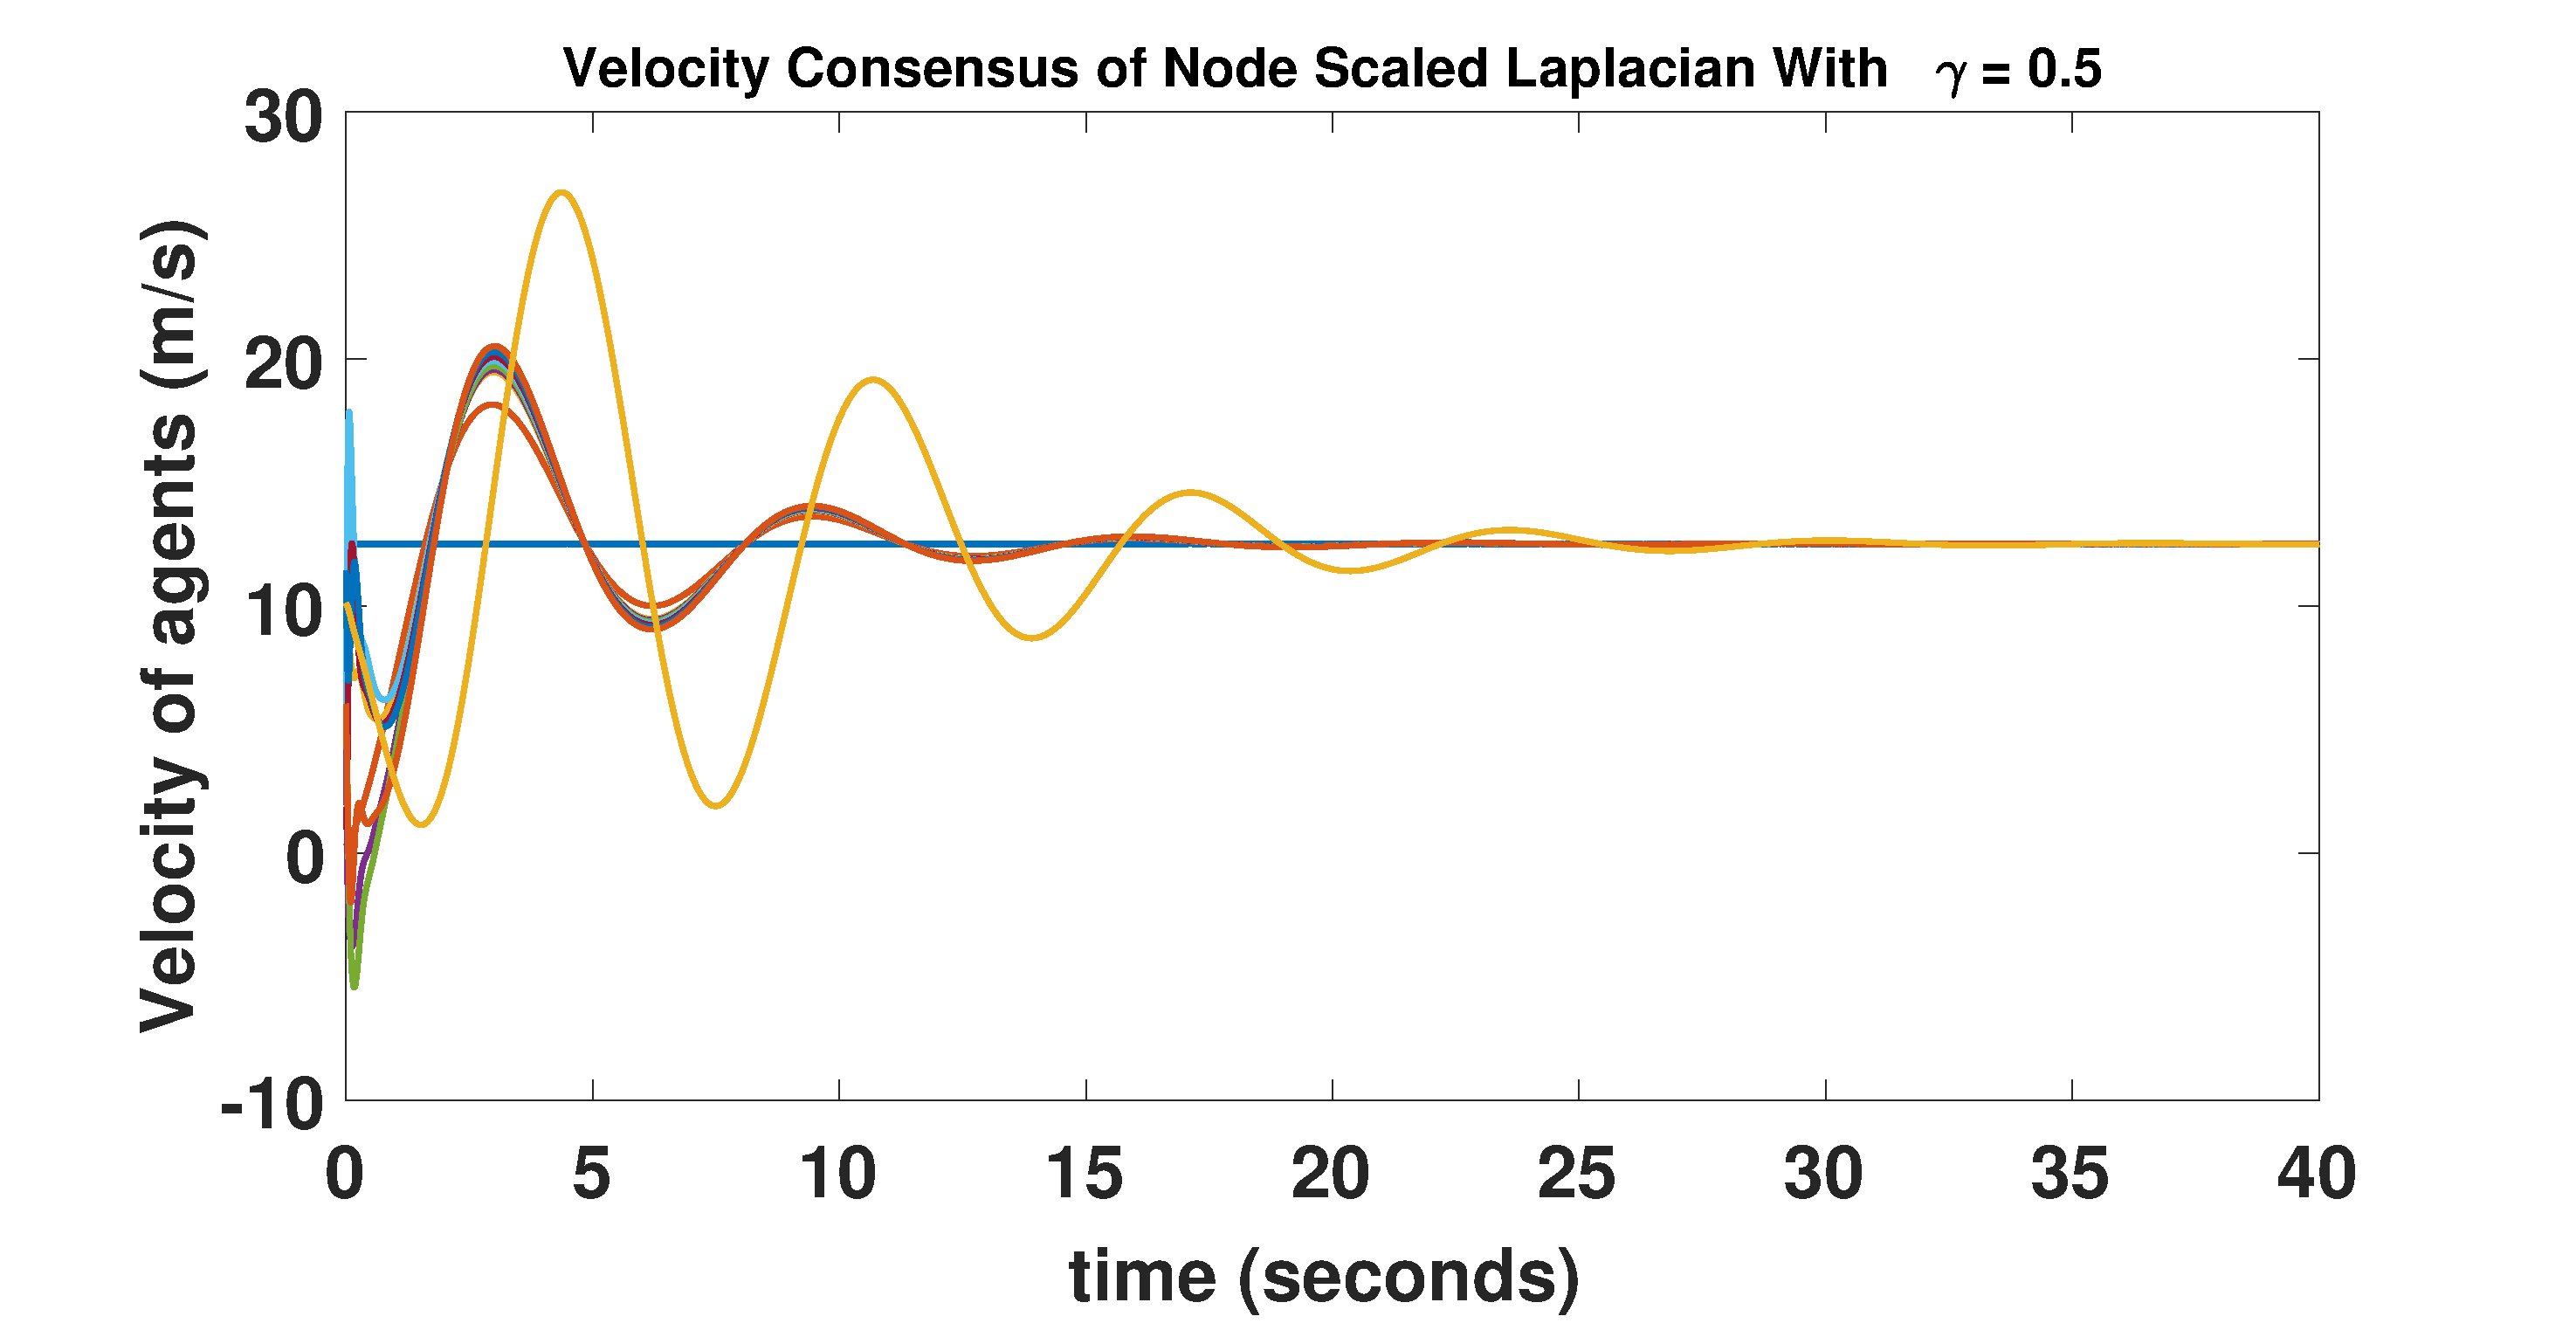
\includegraphics[width=\textwidth, keepaspectratio]{3_Images/10-9-3_NodeScaledLaplacianGamma0.5VelocityConsensus.eps}
		\caption{Node-Scaled Velocity Consensus ($\gamma = 0.5$).}
		\label{fig:10-9-3_NodeScaledLaplacianGamma0.5VelocityConsensus}
	\end{subfigure}
	\caption{Consensus restored using Node-Based Scaling ($p_1 = 31.5, d = 4.5$) under fixed global parameter $\gamma = 0.5$.}
	\label{fig:NodeScaling_sims}
\end{figure}

2. \textbf{Edge-Based Scaling:} Applying Theorem \ref{theo2} with $w_r = 1$, $w_1 \ge 28$. Selecting $w_1 = 31.5$, an AP between $w_1 + w_r = 32.5$ and $w_r = 1$ gives $d = 4.5$, yielding edge weights $\{31.5, 28, 23.5, 19, 14.5, 10, 5.5\}$. The required threshold drops to $\gamma \ge 0.1245 < 0.5$. Figures \ref{fig:10-9-3_ReverseEdgeScaledLaplacianGamma0.5PositionConsensus} and \ref{fig:10-9-3_ReverseEdgeScaledLaplacianGamma0.5VelocityConsensus} demonstrate smooth state convergence.

\begin{figure}[ht!]
	\centering
	\begin{subfigure}[b]{\textwidth}
		\centering
		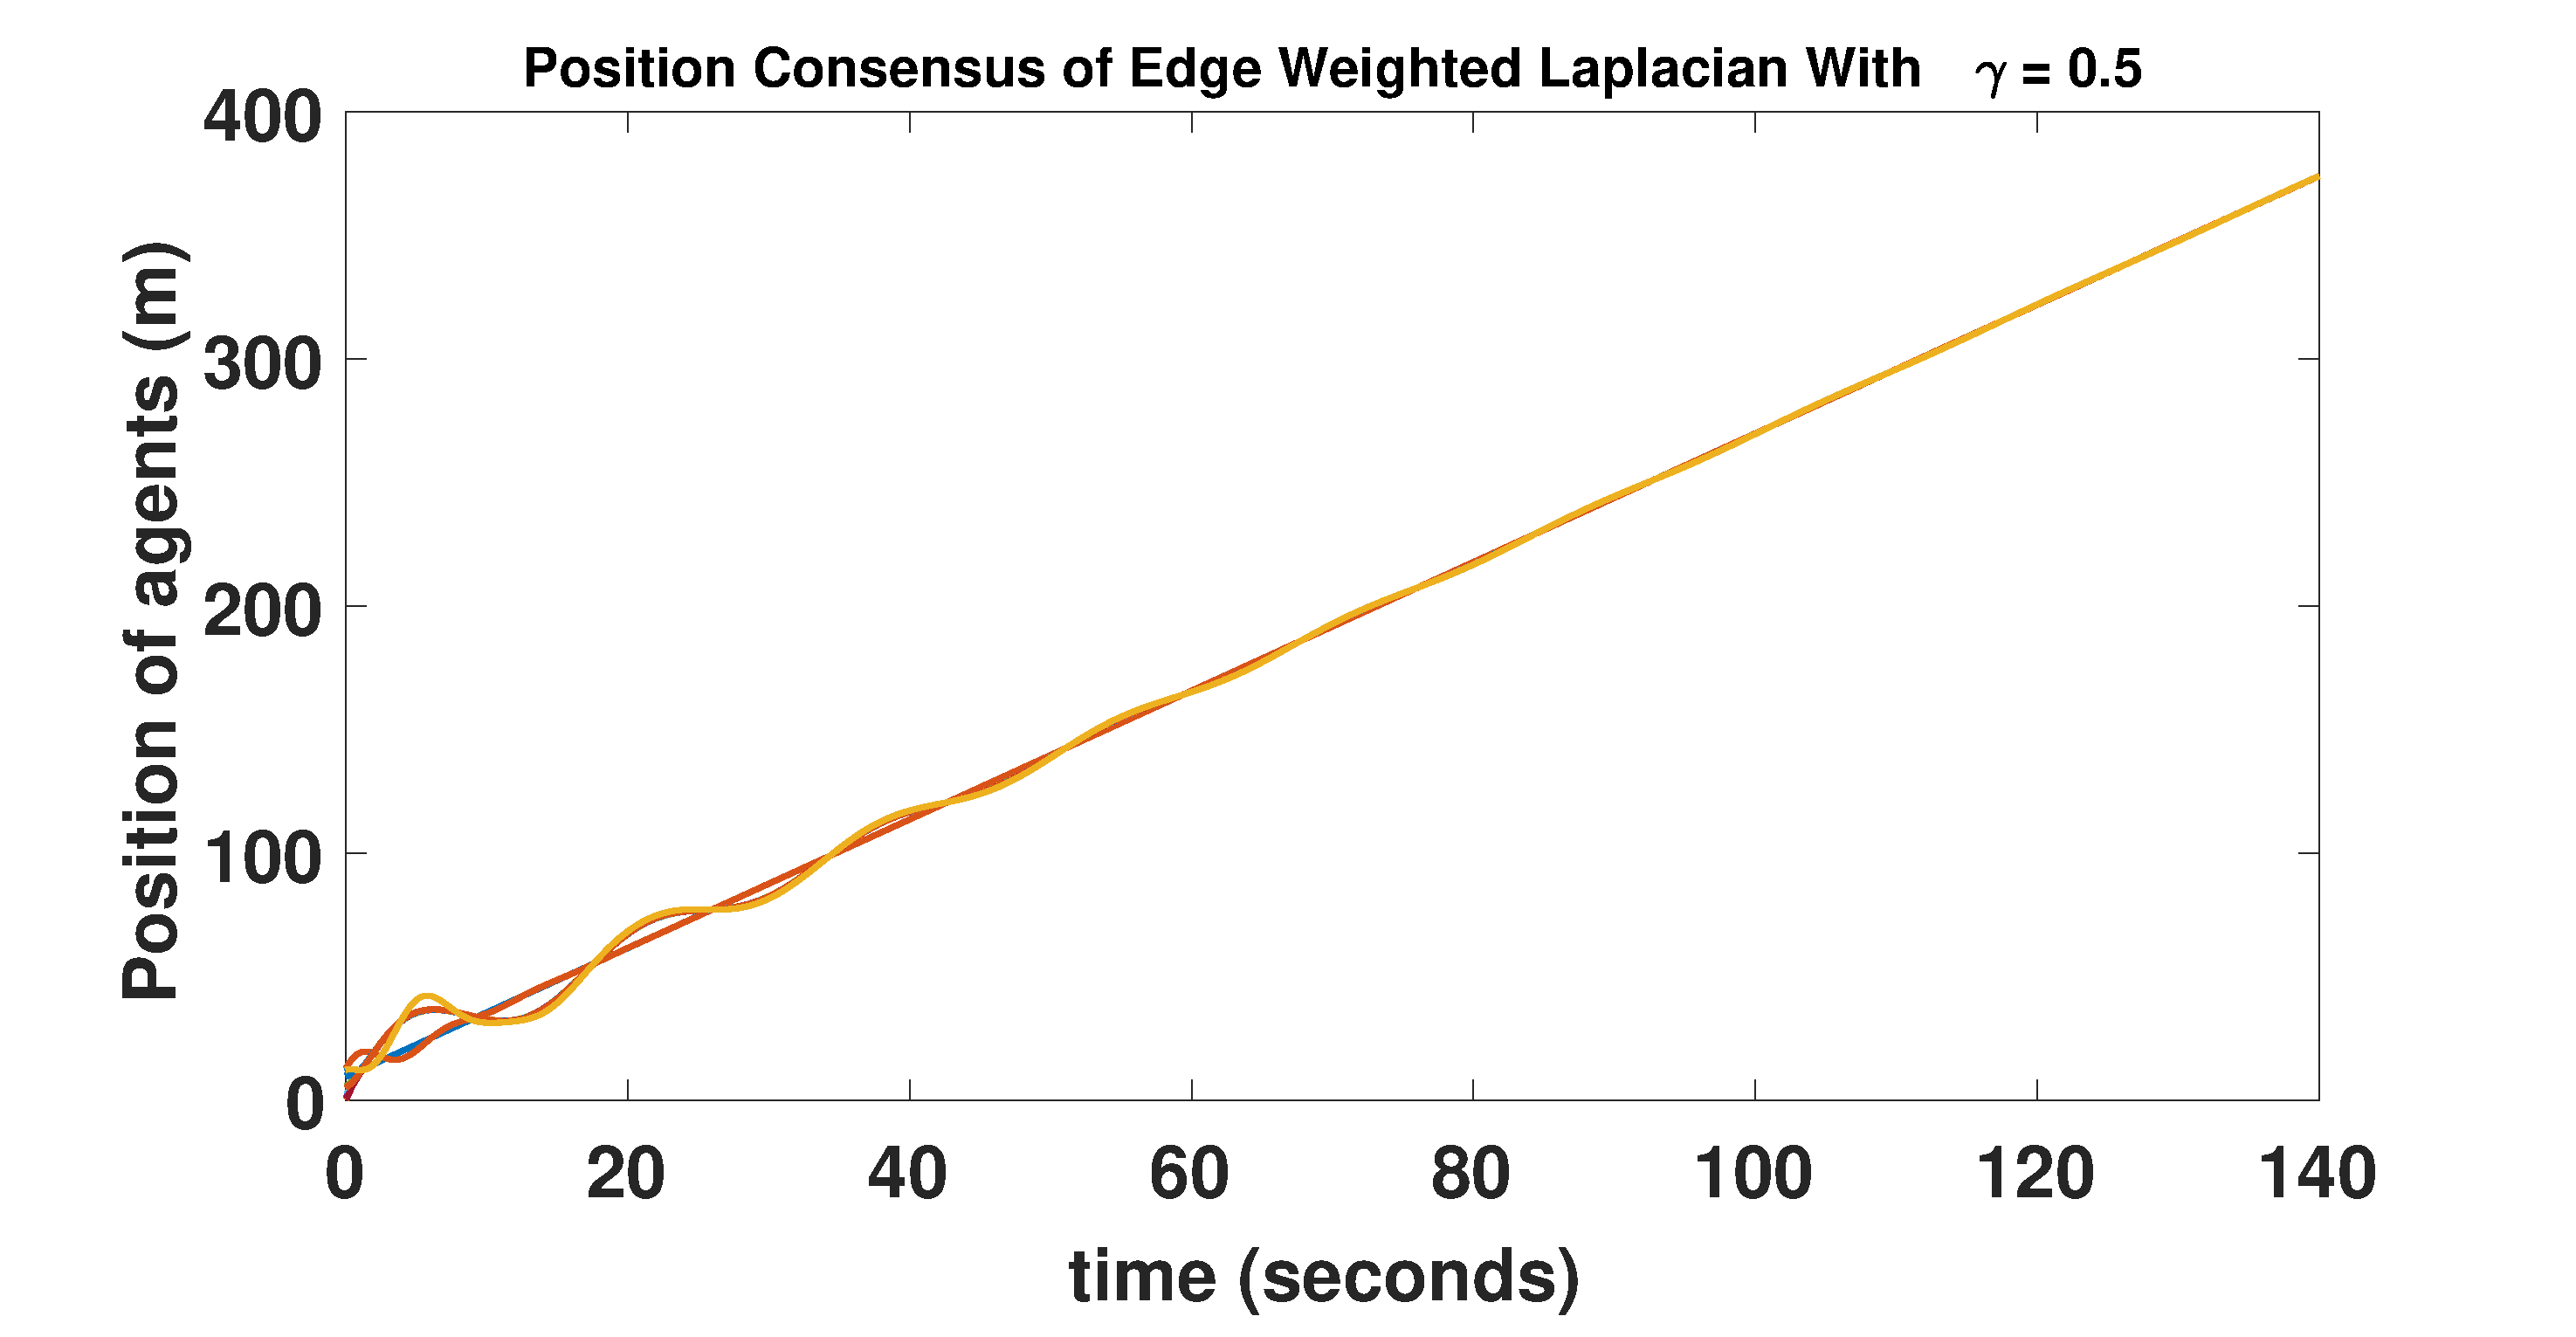
\includegraphics[width=\textwidth, keepaspectratio]{3_Images/10-9-3_ReverseEdgeScaledLaplacianGamma0.5PositionConsensus.eps}
		\caption{Edge-Scaled Position Consensus.}
		\label{fig:10-9-3_ReverseEdgeScaledLaplacianGamma0.5PositionConsensus}
	\end{subfigure}
	\hfill
	\begin{subfigure}[b]{\textwidth}
		\centering
		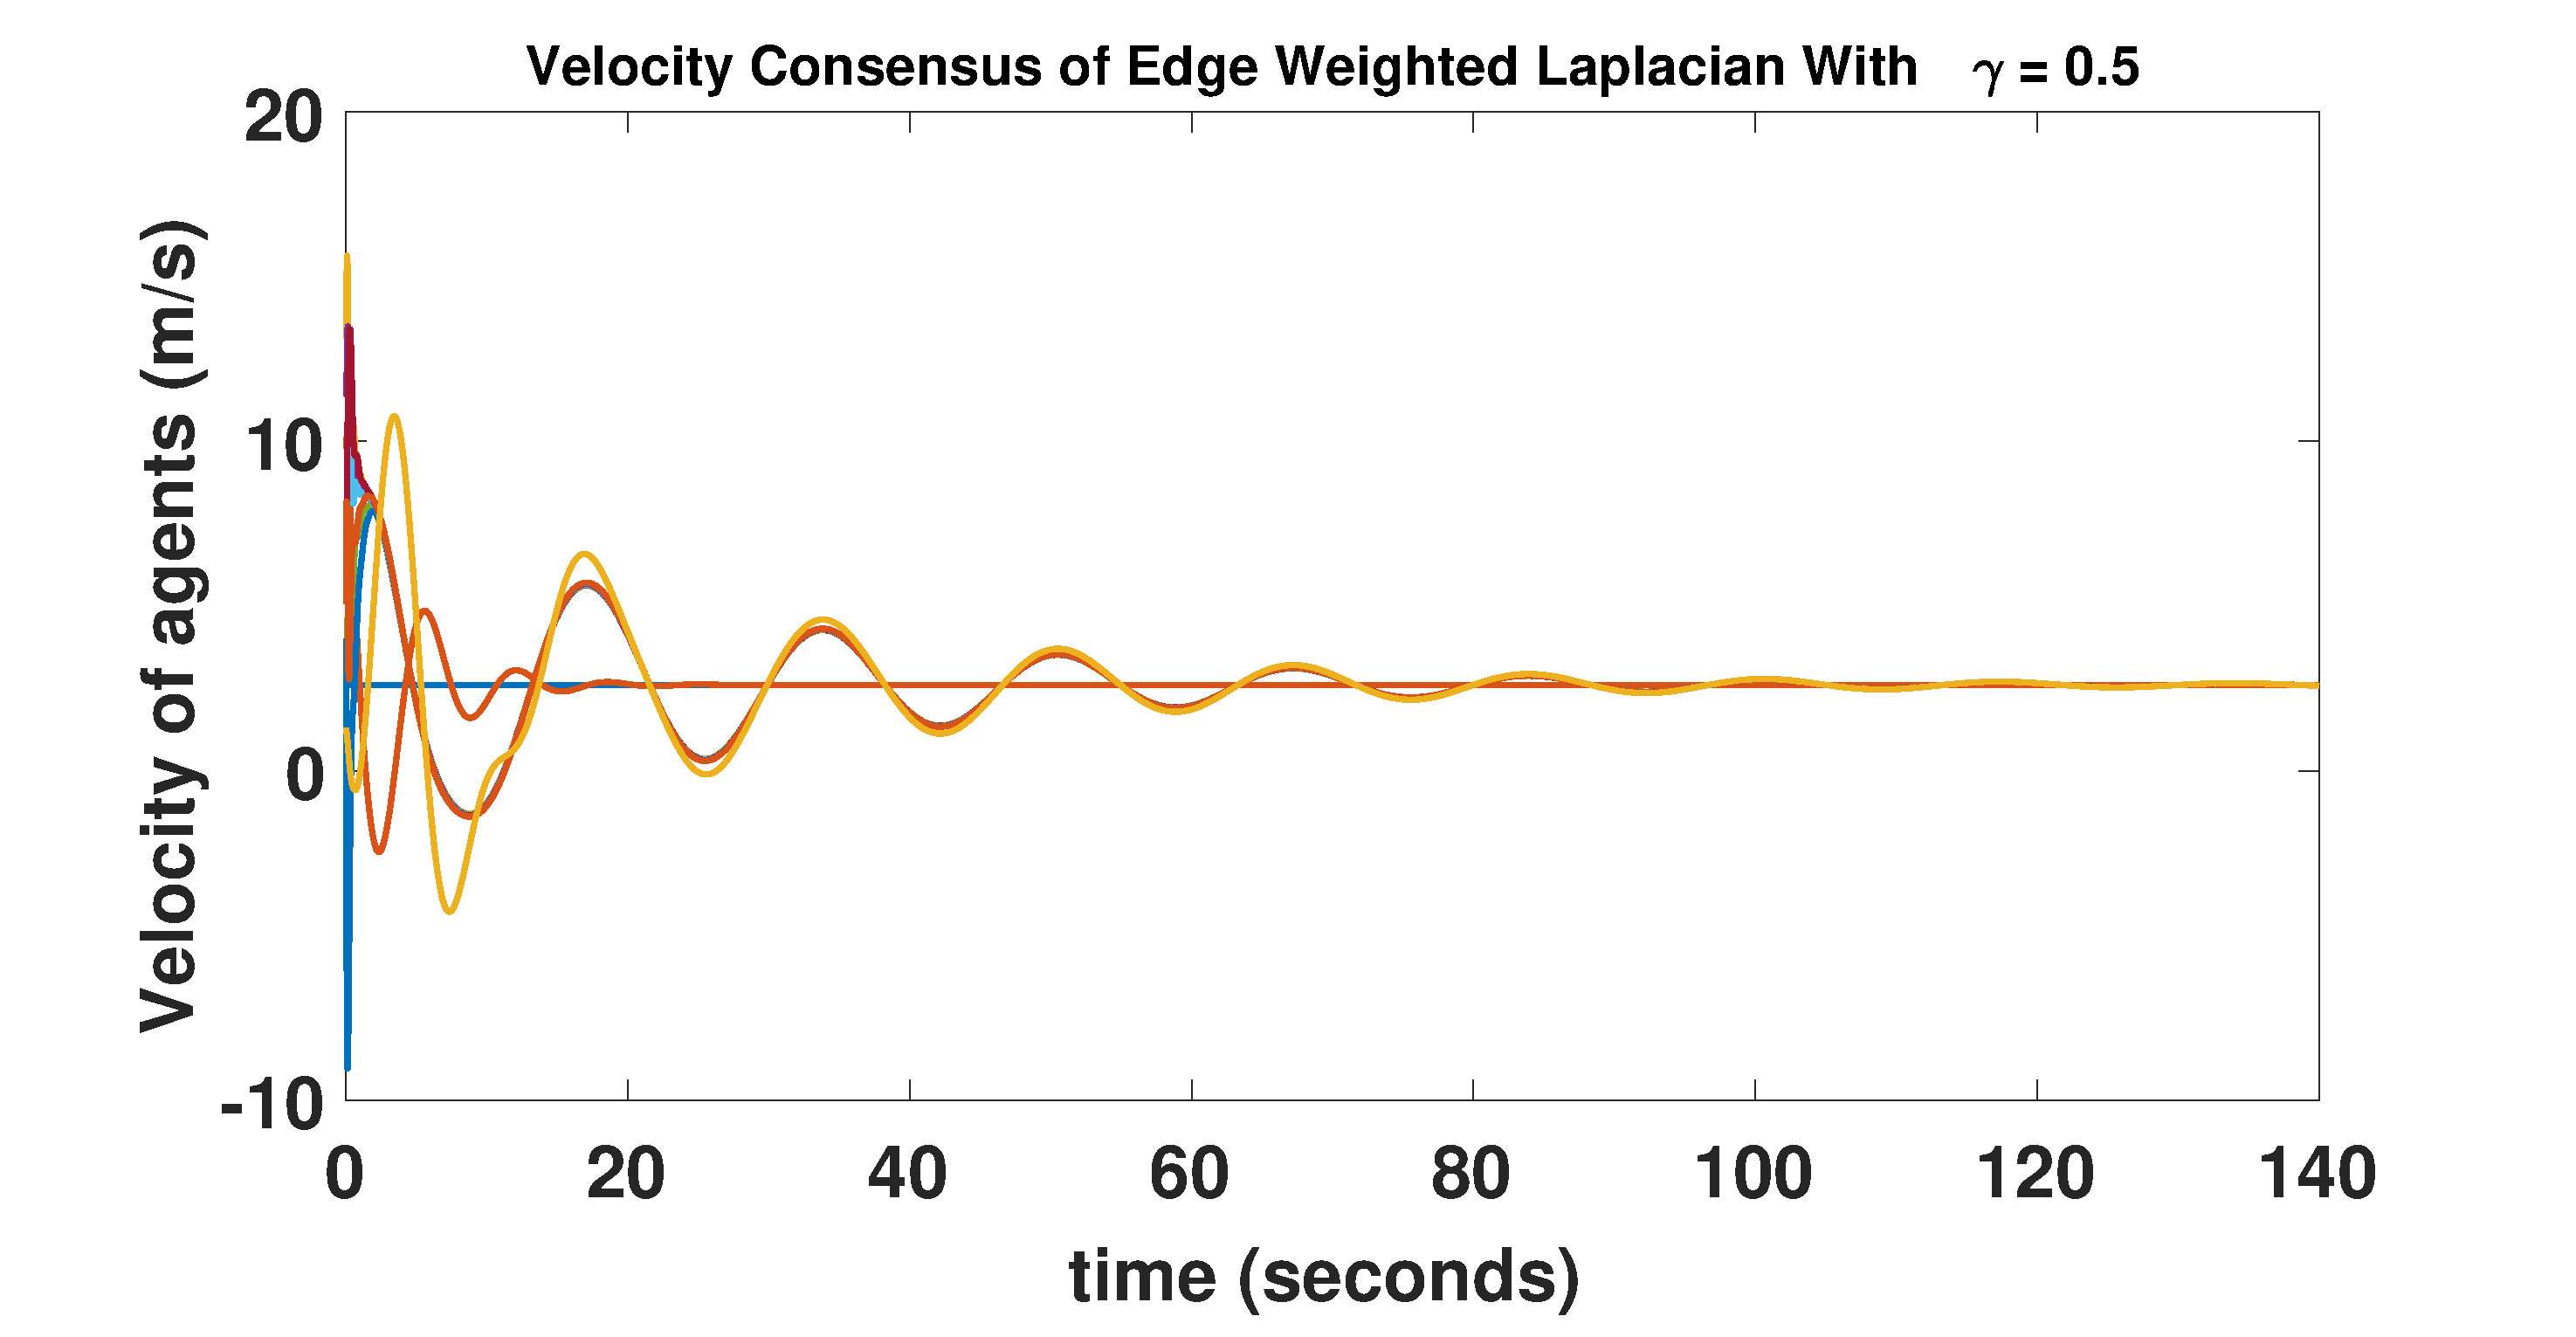
\includegraphics[width=\textwidth, keepaspectratio]{3_Images/10-9-3_ReverseEdgeScaledLaplacianGamma0.5VelocityConsensus.eps}
		\caption{Edge-Scaled Velocity Consensus.}
		\label{fig:10-9-3_ReverseEdgeScaledLaplacianGamma0.5VelocityConsensus}
	\end{subfigure}
	\caption{Consensus restored using Edge-Based Scaling ($w_1 = 31.5, d = 4.5$) under fixed global parameter $\gamma = 0.5$.}
	\label{fig:EdgeScaling_sims}
\end{figure}

3. \textbf{Combined Scaling:} Setting $w_1 = 1$ and $p_1 = 31.5$, edge weights are tuned within the practical hardware range $w_k \in [1, 2]$ ($w_7 = 1.8571, w_6 = 1.7143, w_5 = 1.5714, w_4 = 1.4286, w_3 = 1.2857, w_2 = 1.1429$). The required threshold drops to $\gamma \ge 0.1164 < 0.5$, confirming practical realizability.

\subsection{Validation of Root-Locus Method for Cycle involving the Root Node ($x_1 = 1$)}
Consider a 10-agent network where the reverse edge enters Node 1 ($x_1 = 1, y_1 = 7, \ell = 6$). Fixed coupling is $\gamma = 0.5$. By Theorem \ref{theo3ES}, selecting $\alpha = 9 > 1/\gamma^2 = 4$, the complementary root-locus $G(s) = \frac{\beta\{(s-9)^6 - (-9)^6\}}{s(s-9)^6}$ is plotted in Figures \ref{fig:ComplimentaryRootLocus} and \ref{fig:MirroredComplimentaryRootLocus}. 

The gain margin for stability is $0.6503$. Selecting $\beta = 0.6438$ (giving edge weight $w_2 = \beta / \alpha = 0.0715$), the required threshold drops to $\gamma \ge 0.3501$ which is less than 0.5. Figures \ref{fig:NewRootLocusBasedLaplacianPositionConsensus0.5} and \ref{fig:NewRootLocusBasedLaplacianVelocityConsensus0.5} confirm that second-order consensus is successfully achieved under a root-node loop.

\begin{figure}[ht!]
	\centering
	\begin{subfigure}[b]{\textwidth}
		\centering
		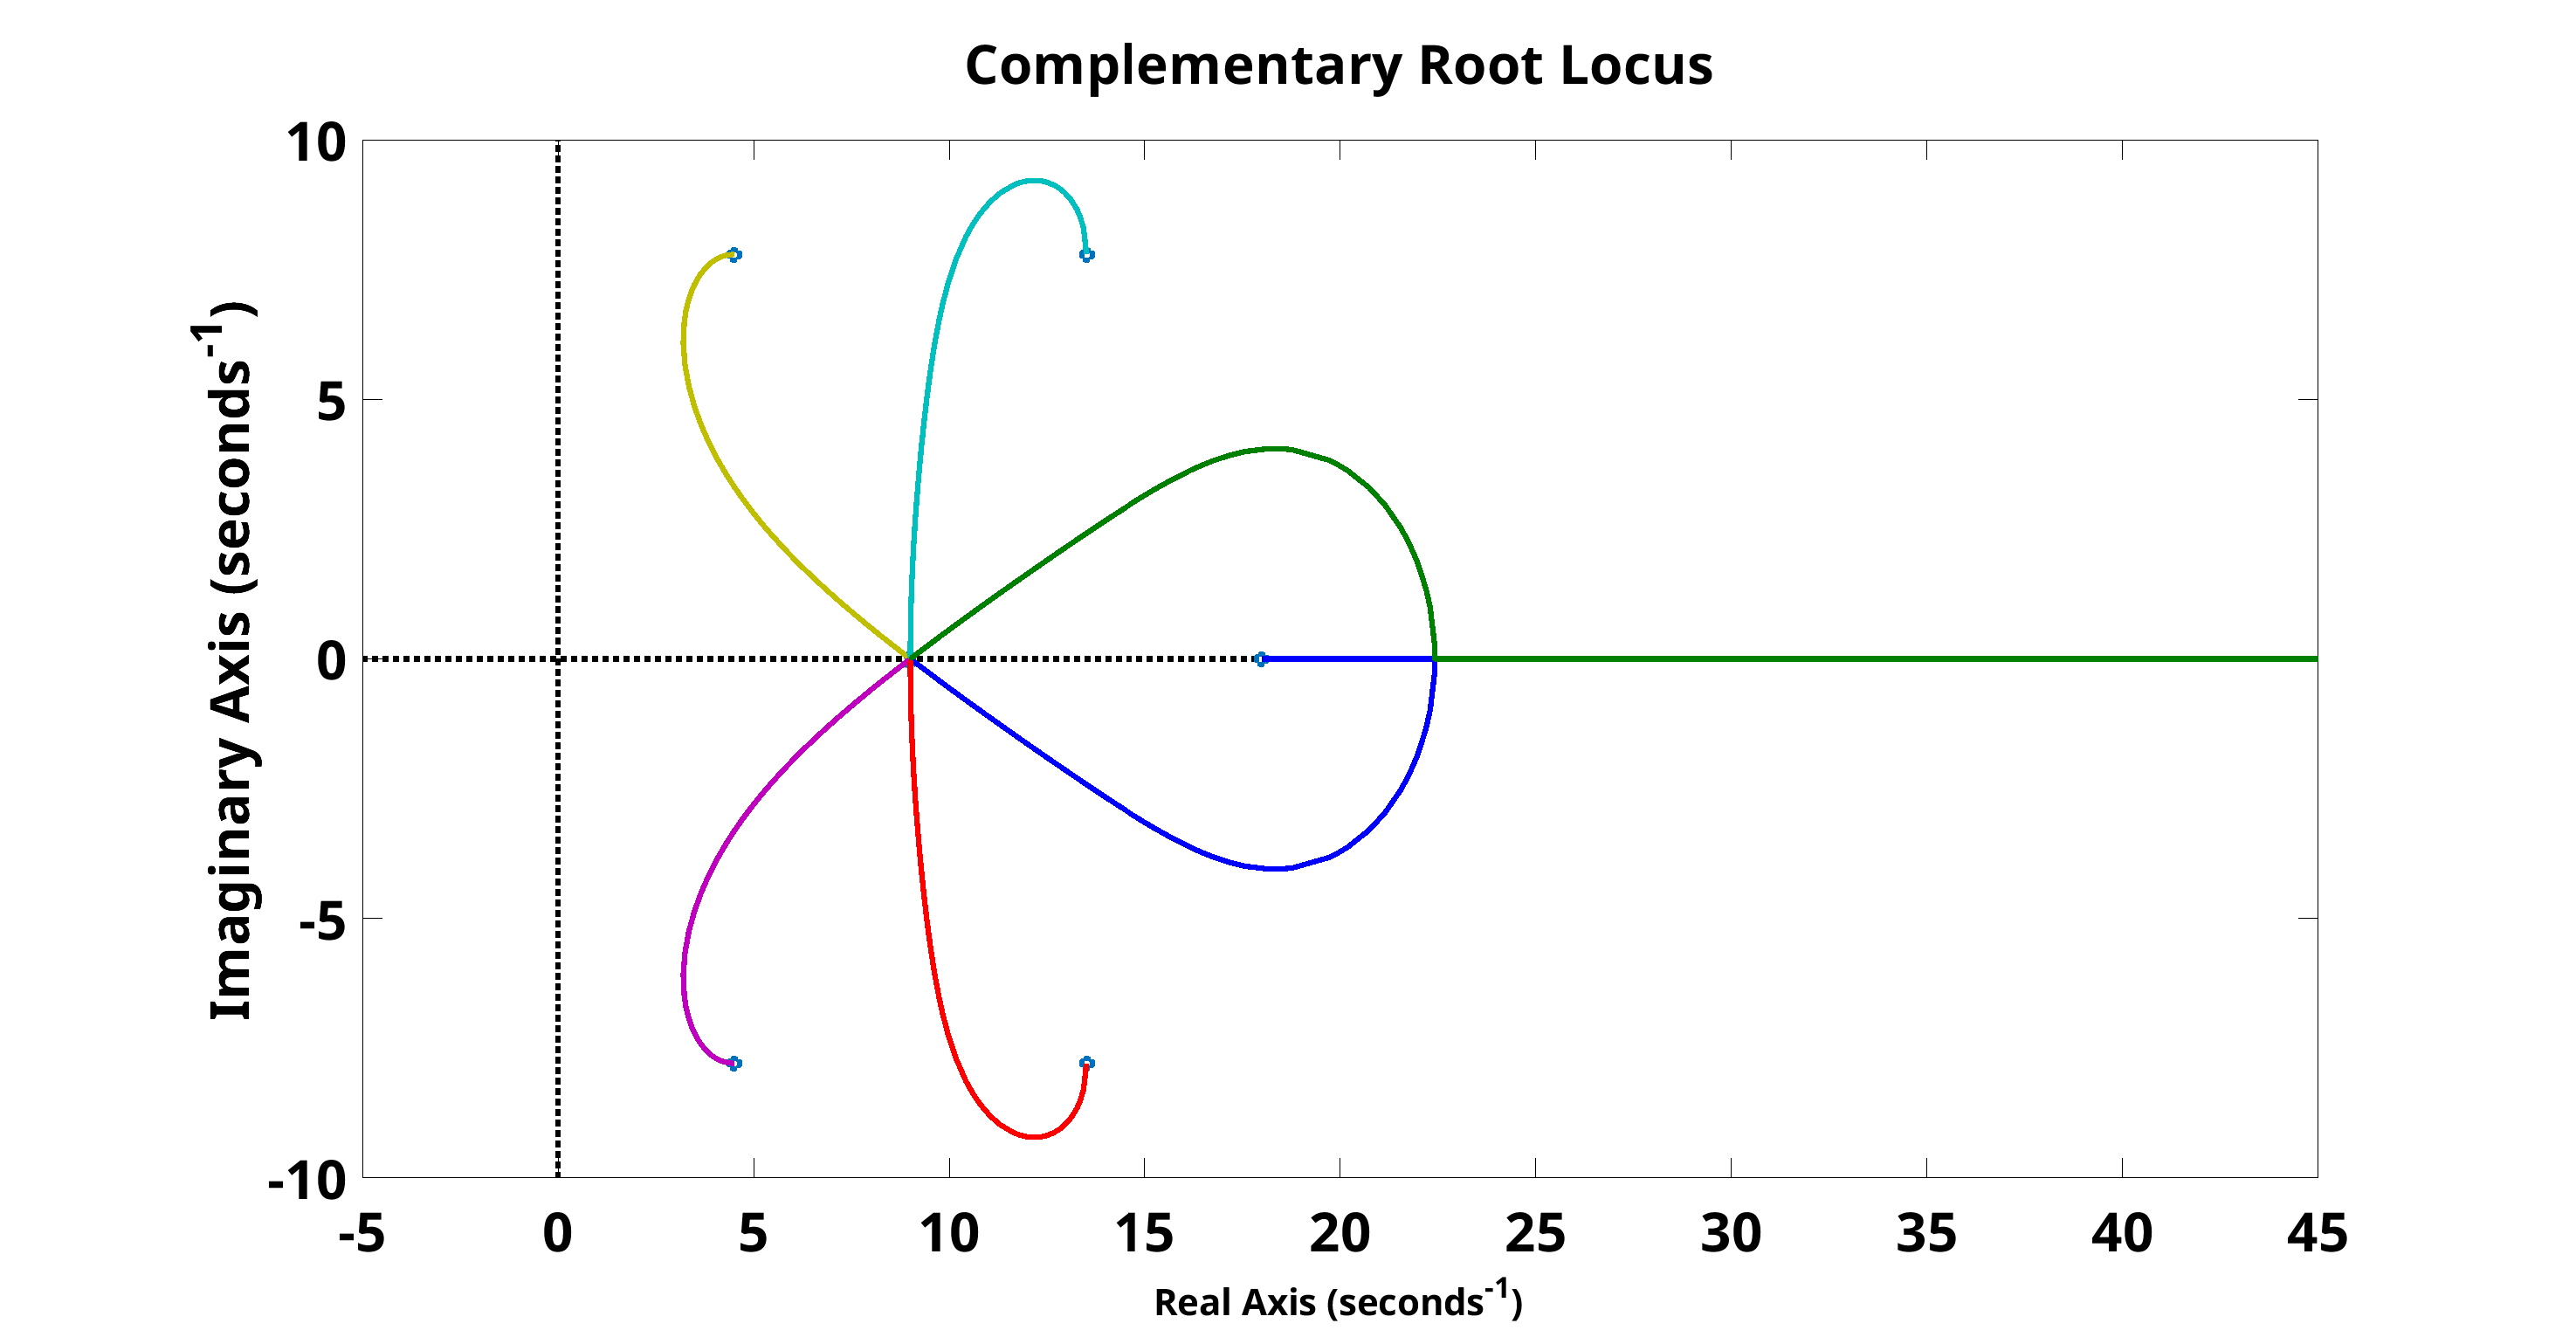
\includegraphics[width=\textwidth, keepaspectratio]{3_Images/CRLwithalpha9.eps}
		\caption{Complementary Root Locus of $G(s)$ for $\alpha = 9$.}
		\label{fig:ComplimentaryRootLocus}
	\end{subfigure}
	\hfill
	\begin{subfigure}[b]{\textwidth}
		\centering
		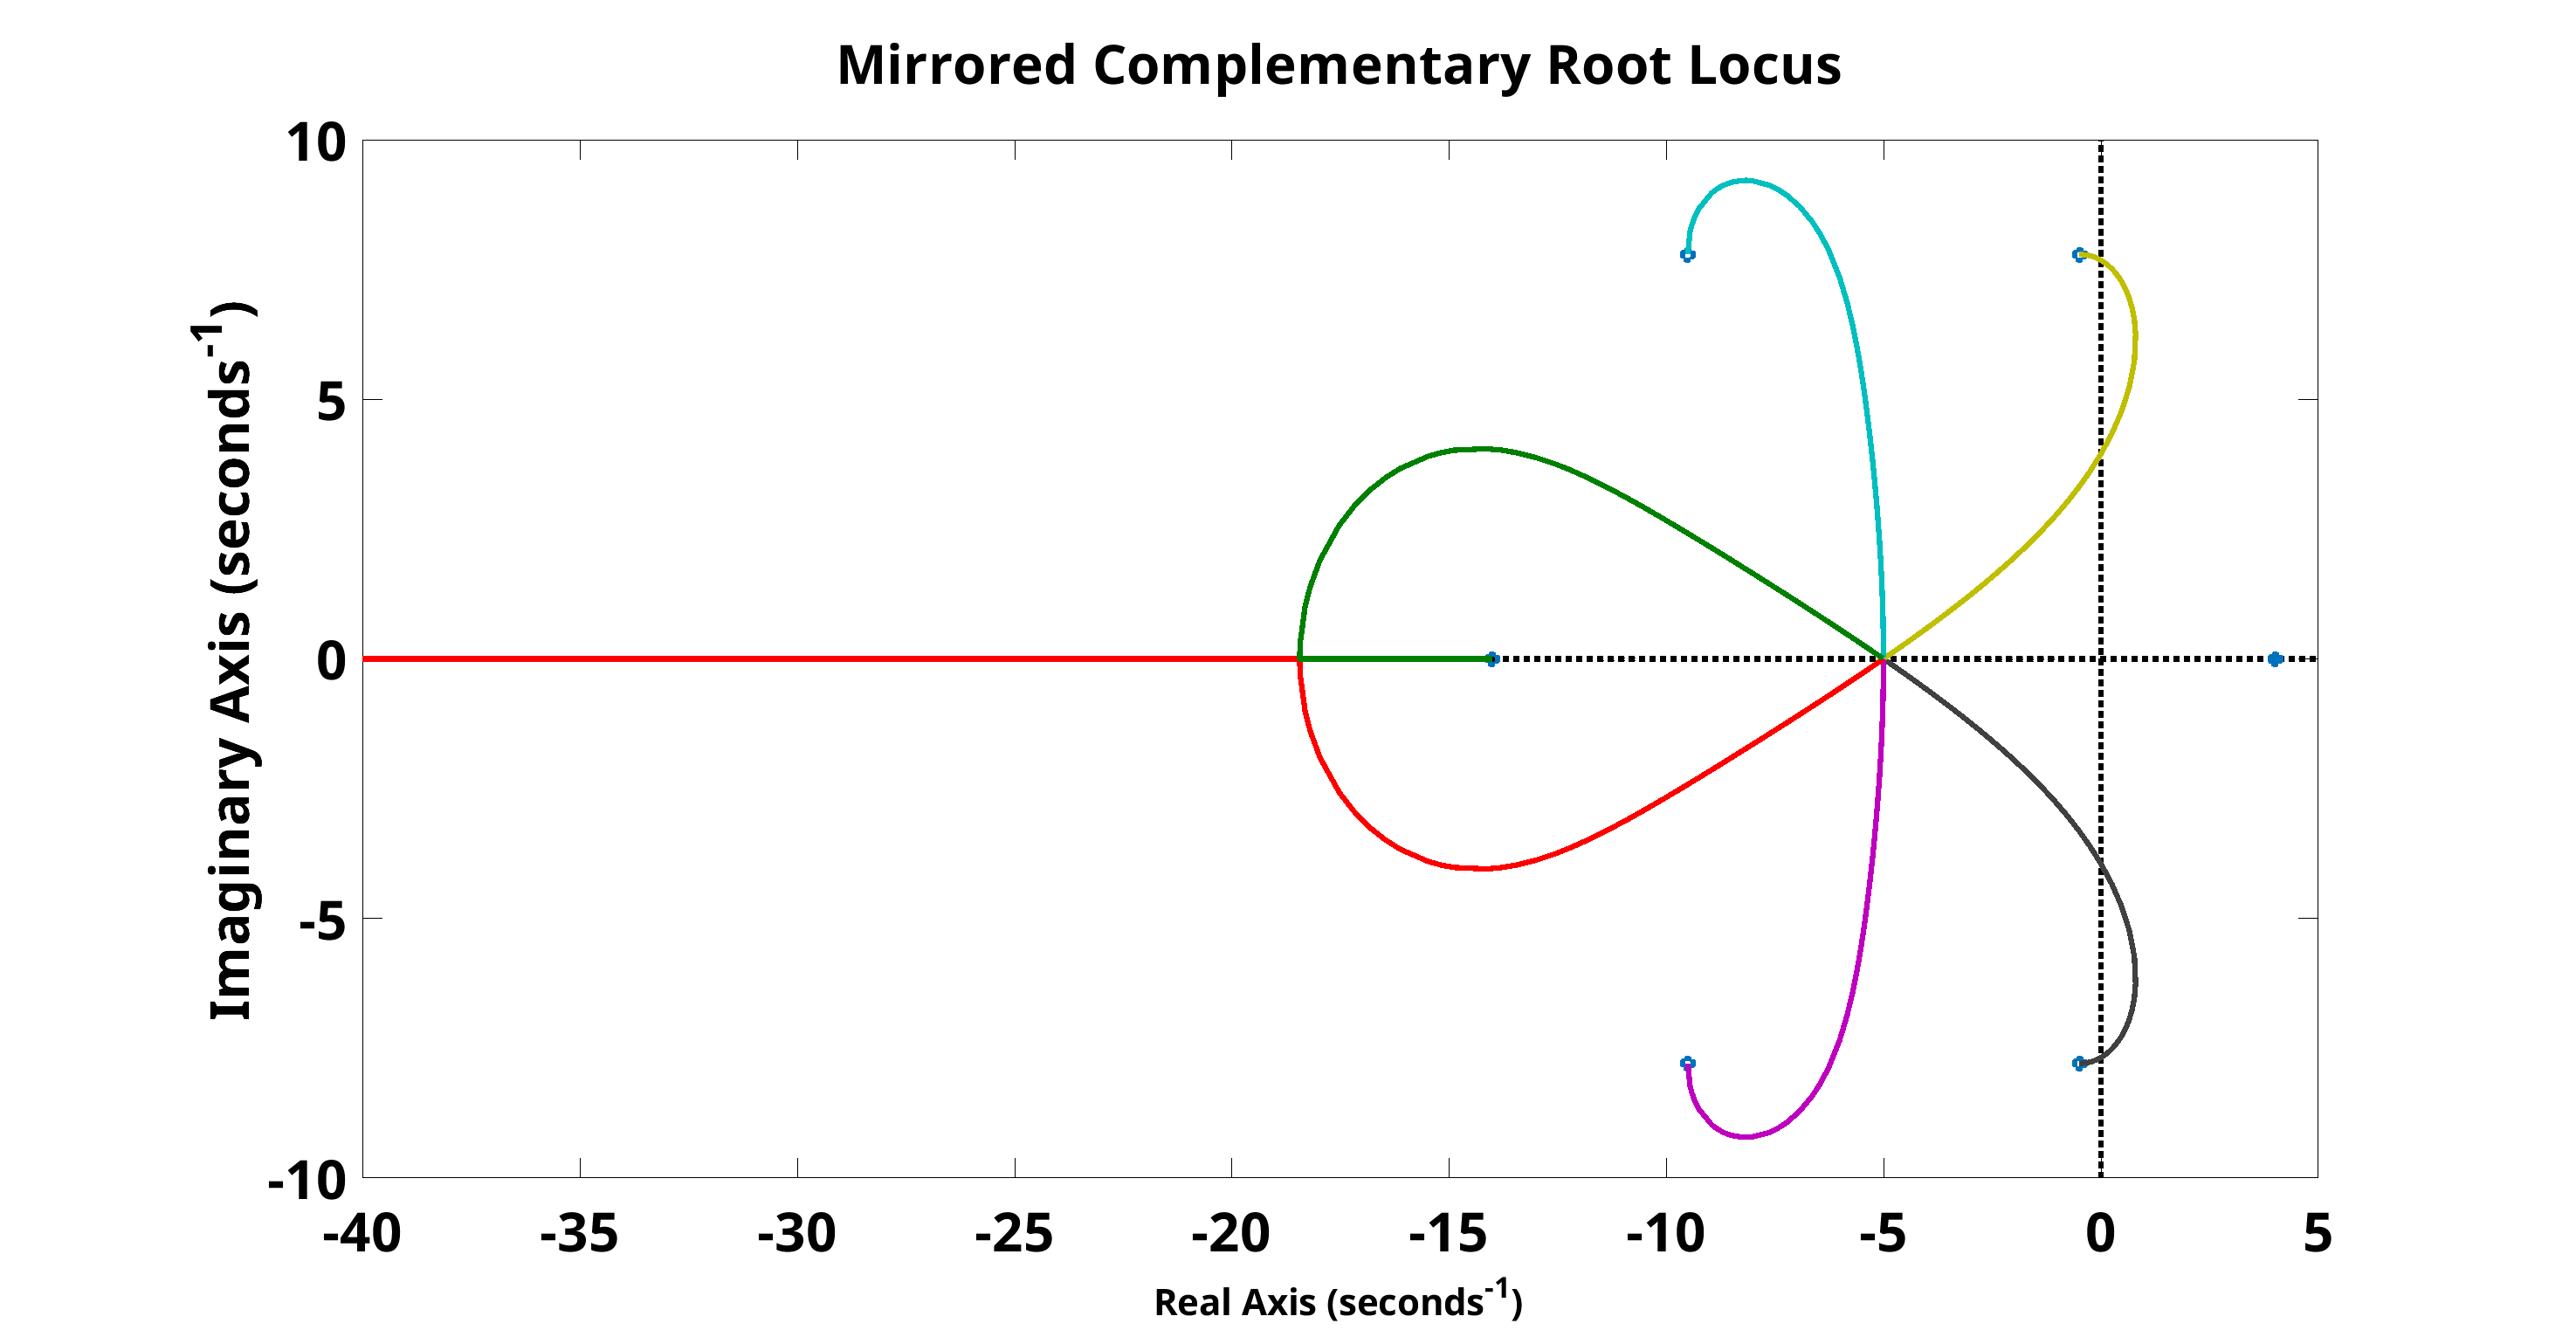
\includegraphics[width=\textwidth, keepaspectratio]{3_Images/NewMirroredCRLShiftedByInverseGammaSquarewithalpha9.eps}
		\caption{Shifted Root Locus bounded by $\mathfrak{Re}(s) = 4$.}
		\label{fig:MirroredComplimentaryRootLocus}
	\end{subfigure}
	\caption{Complementary root locus design for root-node loop ($x_1 = 1, \ell = 6$) under $\alpha = 9$.}
	\label{fig:RootLocus_plots}
\end{figure}

\begin{figure}[ht!]
	\centering
	\begin{subfigure}[b]{\textwidth}
		\centering
		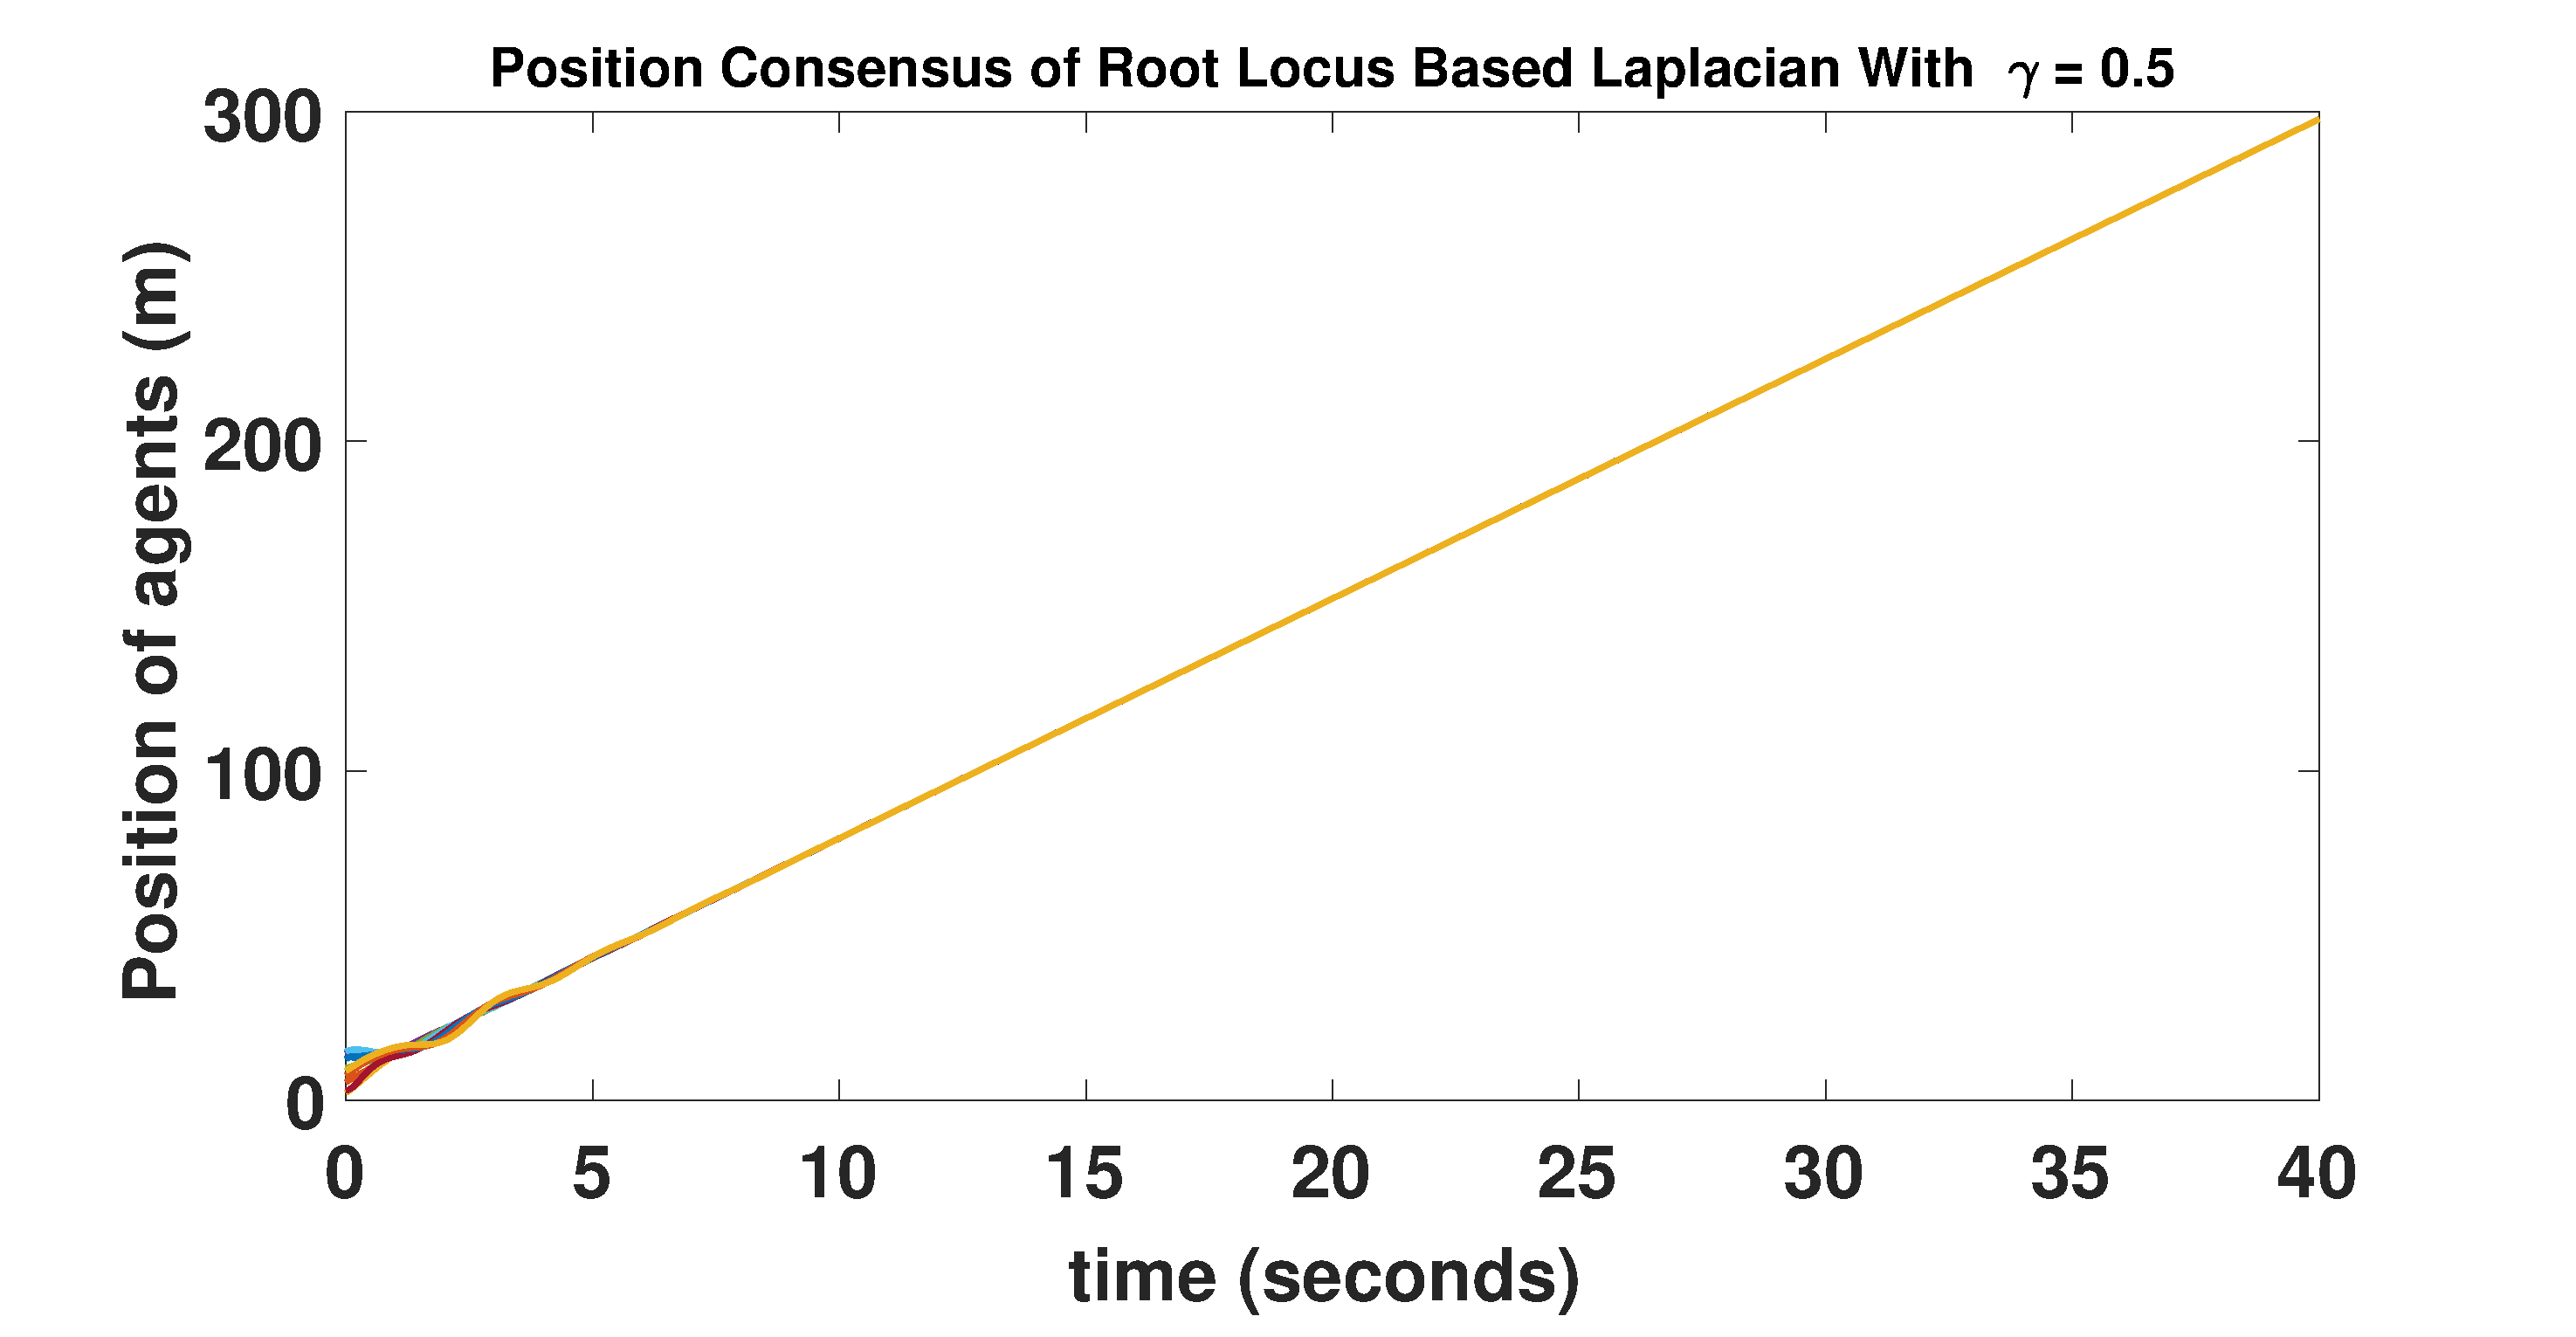
\includegraphics[width=\textwidth, keepaspectratio]{3_Images/NewRLBasedPositionConsensus0.5GammaBetaLessThanGM.eps}
		\caption{Root-Locus Position Consensus ($\gamma = 0.5$).}
		\label{fig:NewRootLocusBasedLaplacianPositionConsensus0.5}
	\end{subfigure}
	\hfill
	\begin{subfigure}[b]{\textwidth}
		\centering
		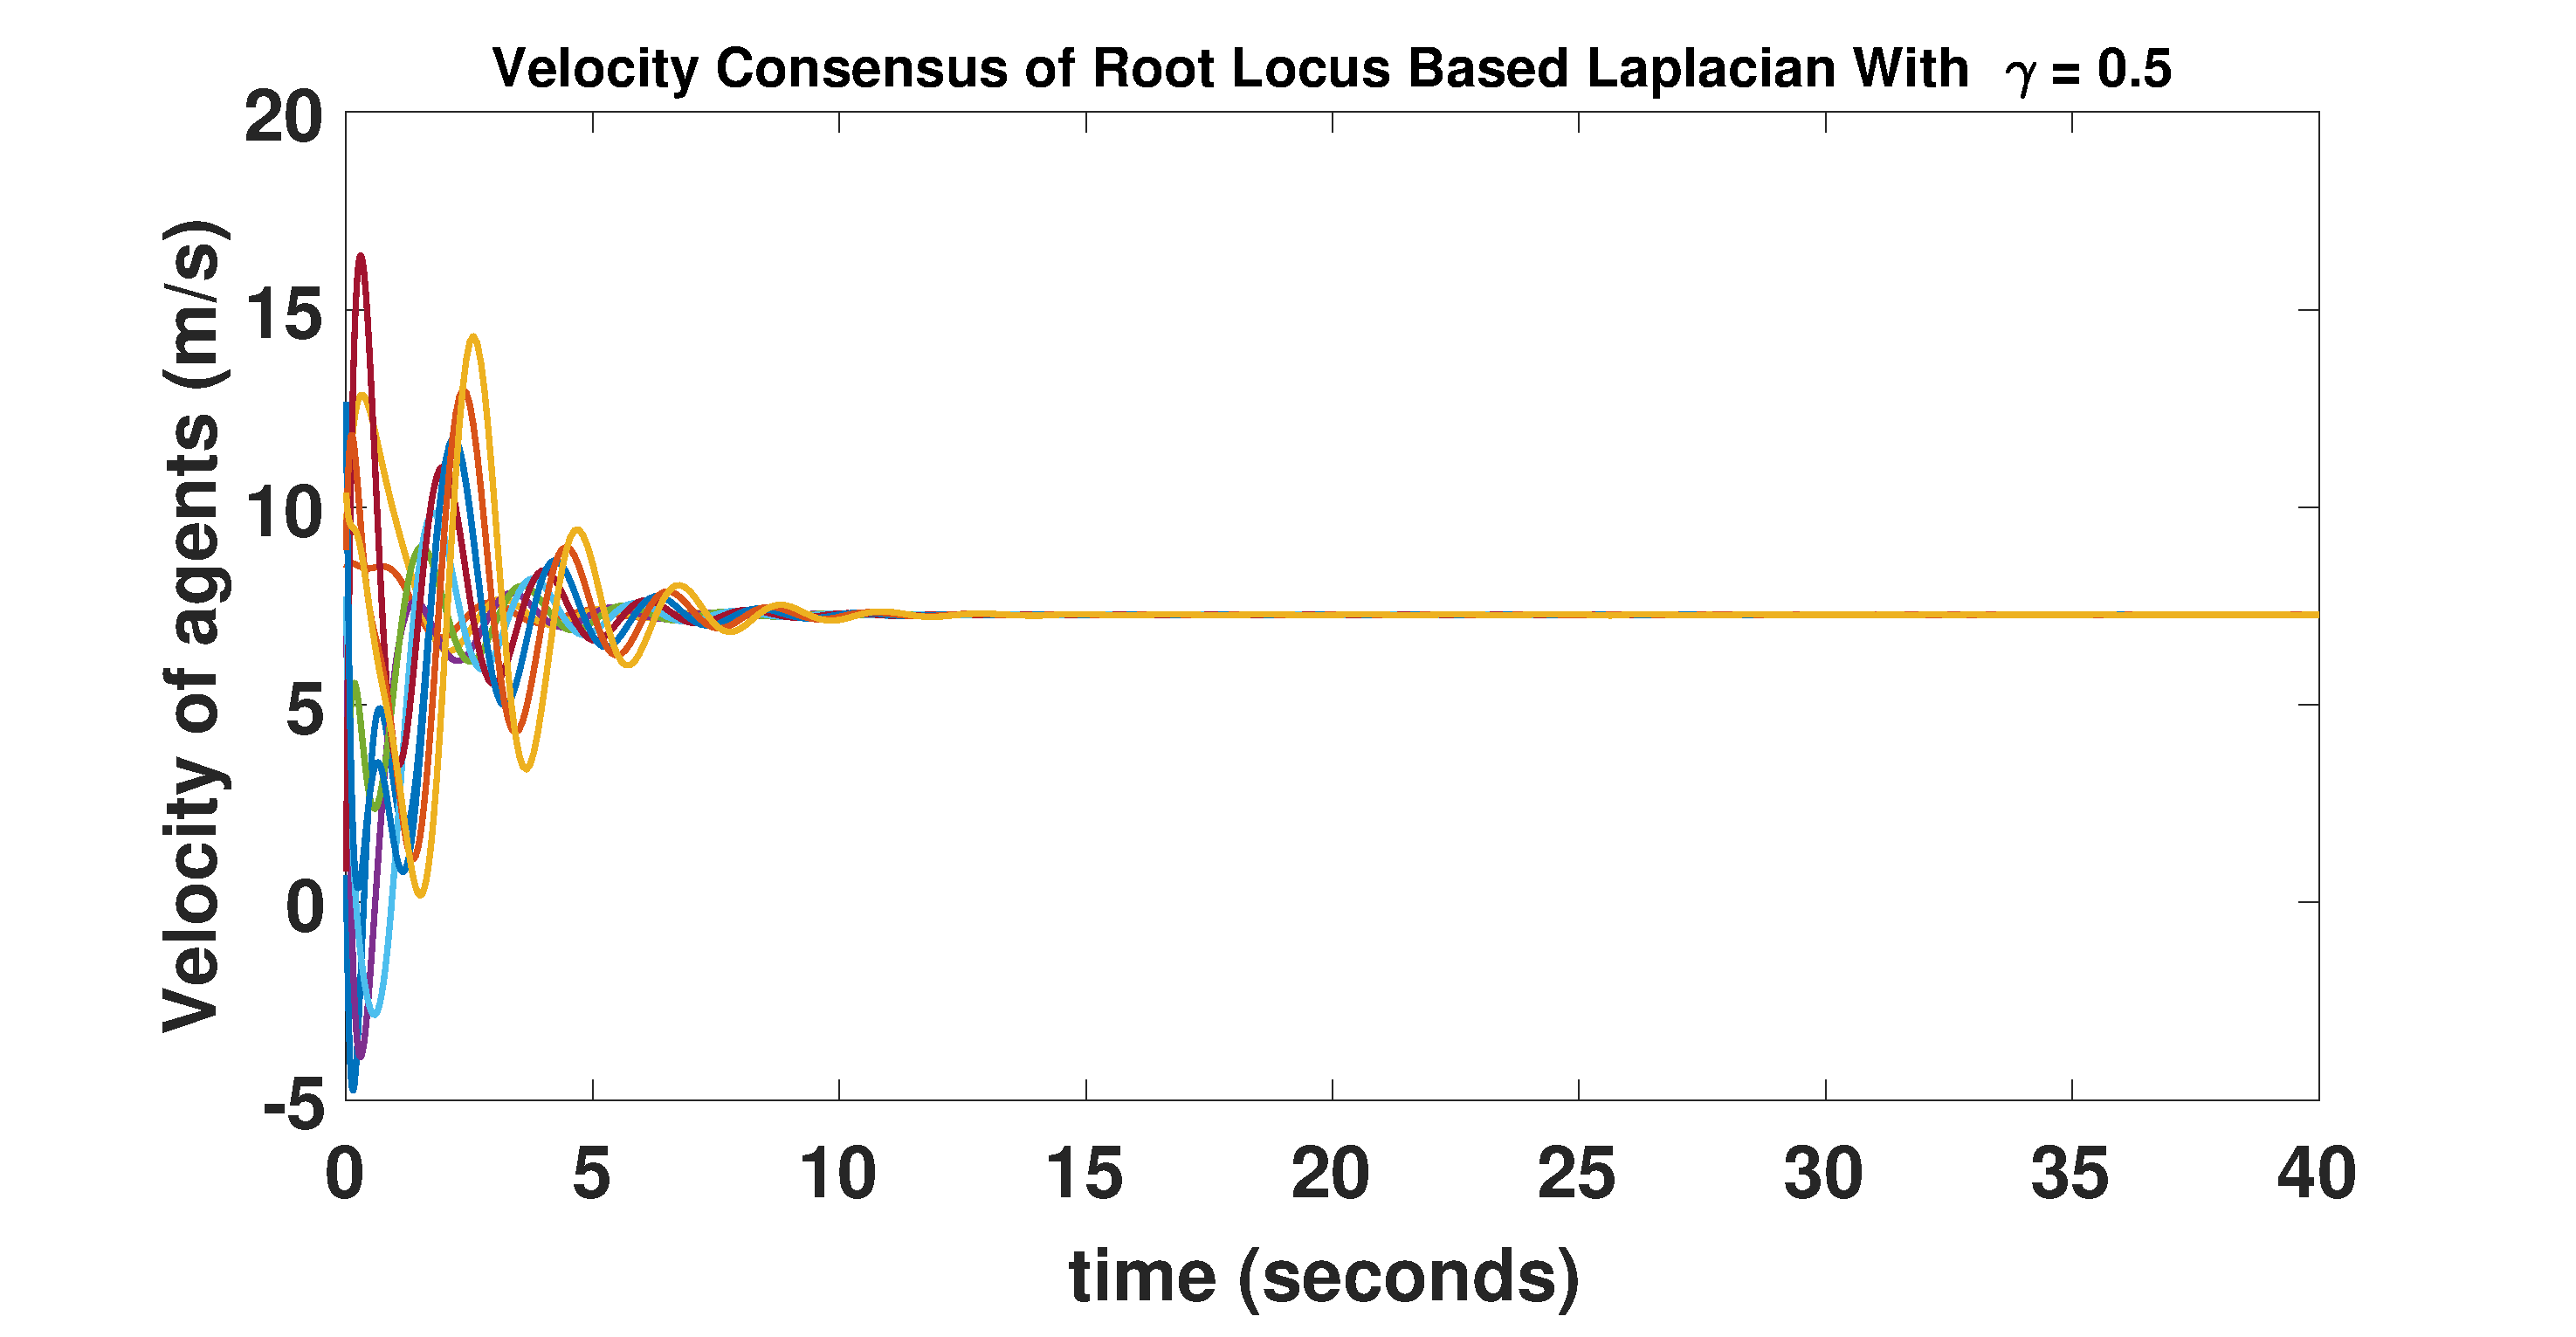
\includegraphics[width=\textwidth, keepaspectratio]{3_Images/NewRLBasedVelocityConsensus0.5GammaBetaLessThanGM.eps}
		\caption{Root-Locus Velocity Consensus ($\gamma = 0.5$).}
		\label{fig:NewRootLocusBasedLaplacianVelocityConsensus0.5}
	\end{subfigure}
	\caption{Position and velocity consensus restored for root-node loop ($x_1 = 1$) using Root-Locus design ($\alpha = 9, \beta = 0.6438$).}
	\label{fig:RootLocus_sims}
\end{figure}

\section{Summary}\label{sec:ch_GC_conclusion}

In this chapter, we presented a number of localized, decentralized control remedies to guarantee second-order consensus in directed chain networks subject to reverse feedback edges, resolving the theoretical limitations identified in Chapter \ref{ch:TwoReverseEdges}. The main contributions are:

\begin{itemize}
    \item \textbf{Gershgorin-Based Local Scaling (Leader-Exterior Loops):} For directed cycles where $x_1 > 1$, we formulated Node-Scaling, Edge-Scaling, and Combined-Scaling algorithms. By establishing that optimal disc separation occurs under an Arithmetic Progression (AP), we proved that tuning local factors to $p_1 \ge (\ell+1)/\gamma^2$ guarantees consensus under fixed global coupling parameters $\gamma$.
    \item \textbf{Root-Locus Remedy (Root-Node Loops):} For directed cycles involving Node 1 ($x_1 = 1$), where polynomial methods collapse, we formulated a complementary root-locus control framework, deriving exact upper bounds on gain $\beta$ that preserve stability.
    \item \textbf{Single-Gain Cyclic Pursuit Synthesis:} To eliminate edge-weakening, we derived a closed-form equal-weight threshold ($\alpha \ge \frac{\cot^2(\pi/(\ell+1))}{2\gamma^2}$) based on cyclic pursuit geometry, guaranteeing consensus without treating any loop edge indifferently.
\end{itemize}
\vspace{0.5em}
\noindent %\textbf{Transition to Chapter \ref{ch:Robustness_Analysis}:}\\
While Chapters \ref{ch:TwoReverseEdges} and \ref{ch:Guaranteed_Consensus} established exact deterministic stability boundaries and localized remedies for cyclic networks, real-world multi-agent systems operate under exogenous process noise and sensor measurement disturbances. 

To evaluate how directed cycles, spatial loop placement, and structural overlap dictate noise propagation and transient energy attenuation, Chapter \ref{ch:Robustness_Analysis} transitions from deterministic stability to systemic performance optimization, utilizing reduced-order edge dynamics ($\Sigma_e$) and suitable Lyapunov equations to derive closed-form expressions for the network $\mathcal{H}_2$ norm.

\chapter[$\mathcal{H}_2$ Performance of Cyclic Networks]{$\mathcal{H}_2$ Performance of a Network of Double-Integrators in Presence of Cycles}\label{ch:Robustness_Analysis}
\section{Introduction}\label{sec:ch_RA_intro}
While Chapter \ref{ch:Guaranteed_Consensus} formulated deterministic local remedies to prevent dynamic divergence and guarantee consensus over a directed network of double-integrators, guaranteeing bounded state agreement is only a baseline requirement. In real-world physical deployments, such as autonomous vehicular platoons and airborne formations subject to wind gusts or sensor noise, multi-agent systems operate under disturbances and noises. Consequently, evaluating how measurement noise and process perturbations propagate across cyclic graphs, using input-output performance metrics such as the $\mathcal{H}_2$ norm, becomes an essential design objective.

Up to this point, our investigations in Chapters \ref{ch:TwoReverseEdges} and \ref{ch:Guaranteed_Consensus} focused exclusively on \emph{directed} communication topologies. In this chapter, we resort to analyzing performance over \emph{undirected} graphs. While undirected networks feature symmetric Laplacian matrices with real spectra, extending $\mathcal{H}_2$ norm performance analysis to second-order agents over undirected cyclic graphs exposes deep, non-trivial combinatorial challenges that do not reveal themselves when agents are modeled as single integrators. Given the rich structural interactions between second-order momentum terms, graph combinatorial properties, and noise propagation, establishing a thorough analytical foundation for undirected double-integrator systems is a necessary and significant prerequisite towards tackling the broader complexity of directed $\mathcal{H}_2$ performance metrics.

A fundamental challenge in evaluating the $\mathcal{H}_2$ performance of consensus protocols is the presence of the zero Laplacian eigenvalue ($\lambda_1 = 0$), which causes the standard controllability Gramian to be unbounded. For single-integrator networks, Zelazo et al. \cite{zelazo2010edge, zelazo2013performance} resolved this singularity using an edge-space projection over reduced-order trees, establishing that adding cycles strictly improves the $\mathcal{H}_2$ norm, quite agnostic to the choice of spanning tree or the spatial location of the cycle. 

However, physical mechanical platforms are governed by Newton's second law of motion, where physical force or acceleration serves as the control input. Extending $\mathcal{H}_2$ performance analysis to double-integrator networks introduces complex cross-coupling between relative position alignment and physical velocity damping. Because double integrators store energy in velocity states, their performance sensitivity to combinatorial graph properties— such as spatial cycle placement and edge overlap— diverges fundamentally from first-order kinematic models. Even under symmetric undirected topologies, double-integrator networks exhibit a strong sensitivity to \emph{where} a cycle is placed and \emph{how much} two cycles overlap— spatial dependencies that are absent in single-integrator consensus.

%While Chapter \ref{ch:Guaranteed_Consensus} formulated deterministic local remedies to prevent dynamic divergence and guarantee consensus stability in double-integrator networks, guaranteeing bounded state agreement is only a baseline requirement. In real-world physical deployments— such as autonomous vehicular platoons and airborne formations subject to wind gusts or sensor drift, multi-agent systems operate under disturbances. Consequently, evaluating how measurement noise and process perturbations propagate across cyclic communication graphs using input-output performance metrics, such as the $\mathcal{H}_2$ norm, becomes an essential design objective.

\subsection*{Summary of Chapter Contributions}
This chapter addresses the aforesaid gap by establishing an exact analytical $\mathcal{H}_2$ performance framework for double-integrators over an undirected network containing cycle(s). The main contributions of this chapter are:
\begin{enumerate}
    \item \textbf{Exact Closed-Form $\mathcal{H}_2$ Norm Expression:} By constructing an edge-space projection $\Sigma_e$ that decouples the unobservable rigid-body drift modes, we derive the exact, closed-form solution to the 2x2 block Lyapunov equation, proving that a double-integrator network always exhibits a larger $\mathcal{H}_2$ norm (poorer noise attenuation) than a single-integrator network.
    \item \textbf{Spanning Tree and Sensitivity to Placement in Network:} Unlike single-integrator systems (where all spanning trees and cycle locations yield identical $\mathcal{H}_2$ performance), we prove that for double integrators, the $\mathcal{H}_2$ norm does depend on the choice of spanning tree and the spatial location of the cycle within the graph. Specifically, placing a cycle near the spatial center of a path graph reduces the system's $\mathcal{H}_2$ norm.
    \item \textbf{Optimal Two-Cycle Overlap Bound:} For networks containing two interacting cycles, we utilize Jensen's Inequality to prove that completely non-overlapping cycles are suboptimal. We derive exact analytical upper bounds on the extent of edge overlap $s \coloneqq  k_1 + k_2$ that guarantees optimal noise suppression.
\end{enumerate}
\section{Graph-Theoretic Preliminaries and Edge Factorizations}\label{sec:ch4_preliminaries}
Let $\mathcal{G} = (\mathcal{V}, \mathcal{E})$ denote a connected, undirected graph with vertex set $\mathcal{V}$ ($|\mathcal{V}| = n$) and edge set $\mathcal{E}$ ($|\mathcal{E}| = e$). Assigning an arbitrary orientation to each edge $k = (i,j) \in \mathcal{E}$, the incidence matrix $E(\mathcal{G}) \in \mathbb{R}^{n \times e}$ is defined component-wise as:
\begin{equation}\label{eq:ch_RA_incidence_def}
	[E(\mathcal{G})]_{ik} = \begin{cases}
		+1, & \text{if vertex } i \text{ is the head of edge } k \\
		-1, & \text{if vertex } i \text{ is the tail of edge } k \\
		0, & \text{otherwise}
	\end{cases}
\end{equation}
The graph Laplacian matrix $\mathcal{L} \in \mathbb{R}^{n \times n}$ is factored as $\mathcal{L} = E(\mathcal{G}) E(\mathcal{G})^T$. 

Select a spanning tree $\mathcal{T} \subset \mathcal{G}$ consisting of $n-1$ tree edges. Partition the incidence matrix as $E(\mathcal{G}) = \begin{bmatrix} E_\tau & E_c \end{bmatrix}$, where $E_\tau \in \mathbb{R}^{n \times (n-1)}$ contains the columns corresponding to spanning tree edges, and $E_c \in \mathbb{R}^{n \times (e-n+1)}$ contains the remaining $e-n+1$ cycle-closing edges. Since the columns of $E_c$ lie in the column space of $E_\tau$, we express $E_c = E_\tau T$, where $T \in \mathbb{R}^{(n-1) \times (e-n+1)}$ is the cycle-basis matrix given by:
\begin{equation}\label{eq:ch_RA_T_matrix}
	T \coloneqq (E_\tau^T E_\tau)^{-1} E_\tau^T E_c
\end{equation}
This yields the fundamental incidence matrix factorization \cite{godsil2001algebraic, zelazo2013performance}:
\begin{equation}\label{eq:ch_RA_incidence_factorization}
	E(\mathcal{G}) = E_\tau \begin{bmatrix} I_{n-1} & T \end{bmatrix} \eqcolon E_\tau R, \quad \text{where } R \coloneqq \begin{bmatrix} I_{n-1} & T \end{bmatrix} \in \mathbb{R}^{(n-1) \times e}
\end{equation}

The tree edge Laplacian $\letree \in \mathbb{R}^{(n-1) \times (n-1)}$ is defined as $\letree \coloneqq E_\tau^T E_\tau$. The essential edge Laplacian $A_3 \in \mathbb{R}^{(n-1) \times (n-1)}$ is defined as:
\begin{equation}\label{eq:ch_RA_A3_def}
	A_3 \coloneqq \letree R R^T = E_\tau^T E(\mathcal{G}) E(\mathcal{G})^T E_\tau (E_\tau^T E_\tau)^{-1}
\end{equation}
Observe that matrix $A_3$ is symmetric, positive definite, and contains all the $(n-1)$ non-zero eigenvalues of the graph Laplacian $\mathcal{L}$.



\section{System Dynamics and Edge-Space Realization}\label{sec:ch_RA_problem_formulation}
In this section, we formulate the noisy state-space model for a networked multi-agent system of double integrators subject to exogenous process disturbances and relative measurement noise. We then construct an explicit coordinate transformation onto an edge-based subspace, eliminating the unobservable rigid-body consensus modes and yielding a minimal, reduced-order realization suitable for $\mathcal{H}_2$ norm computation.

\subsection{Double-Integrator Consensus Model under Noise}

Consider an undirected graph $\mathcal{G} = (\mathcal{V}, \mathcal{E})$ consisting of $n = |\mathcal{V}|$ identical double-integrator agents connected by $e = |\mathcal{E}|$ communication links. The physical translational motion of agent $i \in \{1, 2, \dots, n\}$ is subject to zero-mean, uncorrelated Gaussian process noise $q_i(t) \in \mathbb{R}$ with variance $\mathbb{E}[q_i(t) q_i^T(\tau)] = \sigma_q^2 \delta(t - \tau)$:
\begin{equation}\label{eq:ch_RA_agent_dynamics}
	\dot{x}_i(t) = v_i(t), \quad \dot{v}_i(t) = u_i(t) + q_i(t), \quad i \in \{1, 2, \dots, n\}
\end{equation}
where $x_i(t), v_i(t) \in \mathbb{R}$ denote the scalar position and velocity states of agent $i$, and $u_i(t) \in \mathbb{R}$ represents the control input.

To achieve state agreement over $\mathcal{G}$, agents exchange relative position and relative velocity states with their immediate spatial neighbors. In practical deployments, edge communication channels are corrupted by zero-mean Gaussian measurement noise $r_{ij}(t) \in \mathbb{R}$ with variance $\mathbb{E}[r_{ij}(t) r_{ij}^T(\tau)] = \sigma_r^2 \delta(t - \tau)$. The localized control law $u_i(t)$ incorporating relative measurement noise is defined as:
\begin{equation}\label{eq:ch_RA_control_law}
	u_i(t) = \sum_{j=1}^{n} a_{ij} \left[ (x_j(t) - x_i(t)) + \gamma (v_j(t) - v_i(t)) + r_{ij}(t) \right]
\end{equation}
where $a_{ij} \in \{0, 1\}$ represents the $(i,j)$-th entry of the unweighted adjacency matrix $\mathcal{W}$, and $\gamma > 0$ denotes the global velocity coupling parameter.

To express protocol \eqref{eq:ch_RA_control_law} in compact network coordinates, stack the individual node states, process disturbances, and edge measurement noise into global vectors:
\begin{equation}\label{eq:ch_RA_stackedstates}
	x(t) \coloneqq \begin{bmatrix} x_1(t) \\ \vdots \\ x_n(t) \end{bmatrix} \in \mathbb{R}^n, \quad 
	v(t) \coloneqq \begin{bmatrix} v_1(t) \\ \vdots \\ v_n(t) \end{bmatrix} \in \mathbb{R}^n, \quad 
\end{equation}
\begin{equation}\label{eq:ch_RA_stackednoises}
	q(t) \coloneqq \begin{bmatrix} q_1(t) \\ \vdots \\ q_n(t) \end{bmatrix} \in \mathbb{R}^n, \quad 
	r(t) \coloneqq \begin{bmatrix} r_1(t) \\ \vdots \\ r_e(t) \end{bmatrix} \in \mathbb{R}^e
\end{equation}

Recalling the incidence matrix $E(\mathcal{G}) \in \mathbb{R}^{n \times e}$ from Definition \ref{def:incidence_matrix}, the relative state vector across all $e$ edges can be written as $E^T x(t) \in \mathbb{R}^e$ and $E^T v(t) \in \mathbb{R}^e$. Consequently, the aggregated control vector $u(t) = [u_1(t), \dots, u_n(t)]^T \in \mathbb{R}^n$ expands as:
\begin{align}\label{eq:ch_RA_control_vector}
	u(t) &= -E E^T x(t) - \gamma E E^T v(t) - E r(t) \nonumber \\
	&= -\mathcal{L} x(t) - \gamma \mathcal{L} v(t) - E r(t)
\end{align}
where $\mathcal{L} = E E^T \in \mathbb{R}^{n \times n}$ is the standard graph Laplacian matrix.

Substituting \eqref{eq:ch_RA_control_vector} into the state dynamics \eqref{eq:ch_RA_agent_dynamics} yields the global state equations:
\begin{equation}\label{eq:ch_RA_global_state_eq}
	\begin{aligned}
		\dot{x}(t) &= v(t) \\
		\dot{v}(t) &= -\mathcal{L} x(t) - \gamma \mathcal{L} v(t) + q(t) - E r(t)
	\end{aligned}
\end{equation}

Defining the performance measurement signal $z(t) \in \mathbb{R}^{2e}$ as the vector of relative spatial and velocity displacements across all network edges ($z(t) \coloneqq [(E^T x(t))^T, (E^T v(t))^T]^T$), the full state-space system $\Sigma_n$ with composite state $X(t) \coloneqq [x^T(t), v^T(t)]^T \in \mathbb{R}^{2n}$ is given by:
\begin{equation}\label{eq:ch_RA_system_Sigman}
	\Sigma_n: \begin{cases}
		\dot{X}(t) = \begin{bmatrix} \mathbf{0}_{n \times n} & I_n \\ -\mathcal{L} & -\gamma \mathcal{L} \end{bmatrix} X(t) + \begin{bmatrix} \mathbf{0}_{n \times n} & \mathbf{0}_{n \times e} \\ I_n & -E \end{bmatrix} \begin{bmatrix} q(t) \\ r(t) \end{bmatrix} \\
		z(t) = \begin{bmatrix} E^T & \mathbf{0}_{e \times n} \\ \mathbf{0}_{e \times n} & E^T \end{bmatrix} X(t)
	\end{cases}
\end{equation}

\begin{figure}[ht!]
	\centering
	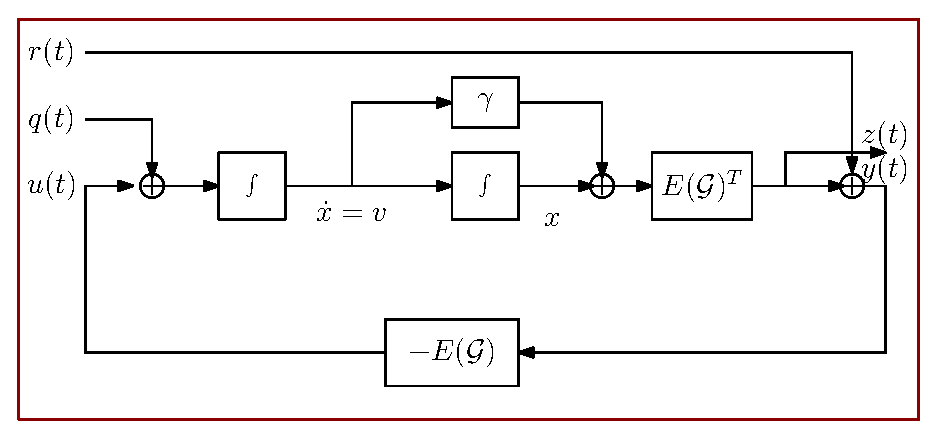
\includegraphics[scale=0.7]{4_Images/double_int_block_undirected.eps}
	\caption{Block diagram representation of the double-integrator network system $\Sigma_n$, depicting feedback loops, process noise $q(t)$, and edge measurement noise $r(t)$.}
	\label{fig:block_double}
\end{figure}
\subsection{Reduced-Order Edge-Space Realization}

System $\Sigma_n$ in \eqref{eq:ch_RA_system_Sigman} cannot be directly evaluated using standard $\mathcal{H}_2$ norm computation methods. Because the connected graph Laplacian $\mathcal{L}$ possesses a simple zero eigenvalue ($\lambda_1 = 0$) with right eigenvector $\mathbf{1}_n = [1, 1, \dots, 1]^T \in \mathbb{R}^n$, system $\Sigma_n$ contains two unobservable, non-stationary rigid-body modes corresponding to the average network position $\frac{1}{n} \mathbf{1}_n^T x(t)$ and average network velocity $\frac{1}{n} \mathbf{1}_n^T v(t)$. These drift modes cause the controllability Gramian of $\Sigma_n$ to be undefined ($X^* \to \infty$).

To project the network dynamics onto a stable subspace and eliminate these unobservable modes, we select a spanning tree $\mathcal{T} \subset \mathcal{G}$ consisting of $(n-1)$ tree edges. Using the incidence matrix factorization \eqref{eq:ch_RA_incidence_factorization} $E(\mathcal{G}) = E_\tau R = E_\tau \begin{bmatrix} I_{n-1} & T \end{bmatrix}$ from \eqref{eq:incidence_factored}, we introduce the linear spatial coordinate transformation matrix $S_v \in \mathbb{R}^{n \times n}$:
\begin{equation}\label{eq:ch_RA_transformation_Sv}
	S_v \coloneqq \begin{bmatrix} E_\tau (E_\tau^T E_\tau)^{-1} & \frac{1}{n} \mathbf{1}_n \end{bmatrix} = \begin{bmatrix} E_\tau \letree^{-1} & \frac{1}{n} \mathbf{1}_n \end{bmatrix}
\end{equation}
where $\letree = E_\tau^T E_\tau \in \mathbb{R}^{(n-1) \times (n-1)}$ is the positive-definite tree edge Laplacian matrix.

Applying $S_v$ to transform the nodal position and velocity vectors we have the following relationship:
\begin{equation}\label{eq:ch_RA_coordinate_change}
	x(t) = S_v x_e(t) = \begin{bmatrix} E_\tau \letree^{-1} & \frac{1}{n} \mathbf{1}_n \end{bmatrix} \begin{bmatrix} x_\tau(t) \\ x_\mathbf{1}(t) \end{bmatrix}, \quad 
	v(t) = S_v v_e(t) = \begin{bmatrix} E_\tau \letree^{-1} & \frac{1}{n} \mathbf{1}_n \end{bmatrix} \begin{bmatrix} v_\tau(t) \\ v_\mathbf{1}(t) \end{bmatrix}
\end{equation}
where $x_\tau(t) \coloneqq E_\tau^T x(t) \in \mathbb{R}^{n-1}$ and $v_\tau(t) \coloneqq E_\tau^T v(t) \in \mathbb{R}^{n-1}$ represent the relative position and velocity state vectors along the $n-1$ chosen spanning tree edges, while $x_\mathbf{1}(t) \coloneqq \mathbf{1}_n^T x(t) \in \mathbb{R}$ and $v_\mathbf{1}(t) \coloneqq \mathbf{1}_n^T v(t) \in \mathbb{R}$ denote the scalar centroid (average) modes.

Taking the inverse of transformation matrix $S_v$:
\begin{equation}\label{eq:ch_RA_Sv_inverse}
	S_v^{-1} = \begin{bmatrix} E_\tau^T \\ \mathbf{1}_n^T \end{bmatrix} \in \mathbb{R}^{n \times n},
\end{equation}
and pre-multiplying global state equations \eqref{eq:ch_RA_global_state_eq} by $S_v^{-1}$ separates out the relative edge coordinates as follows:.

\begin{enumerate}
	\item \textbf{Relative Tree Edge Dynamics ($x_\tau, v_\tau$):}
	\begin{align}\label{eq:ch_RA_edge_dynamics_raw}
		\dot{x}_\tau(t) &= E_\tau^T v(t) = v_\tau(t) \nonumber \\
		\dot{v}_\tau(t) &= E_\tau^T \dot{v}(t) = -E_\tau^T \mathcal{L} x(t) - \gamma E_\tau^T \mathcal{L} v(t) + E_\tau^T q(t) - E_\tau^T E r(t)
	\end{align}
	Substituting $\mathcal{L} = E E^T = E_\tau R R^T E_\tau^T$ into $E_\tau^T \mathcal{L} x(t)$:
	\begin{equation}
		E_\tau^T \mathcal{L} x(t) = (E_\tau^T E_\tau) R R^T (E_\tau^T x(t)) = \letree R R^T x_\tau(t) = A_3 x_\tau(t)
	\end{equation}
	where $A_3 \coloneqq \letree R R^T \in \mathbb{R}^{(n-1) \times (n-1)}$ is the essential edge Laplacian matrix introduced in \eqref{eq:ch_RA_A3_def}. Similarly, $E_\tau^T \mathcal{L} v(t) = A_3 v_\tau(t)$, and $E_\tau^T E r(t) = E_\tau^T E_\tau R r(t) = \letree R r(t)$. Thus:
	\begin{equation}\label{eq:ch_RA_v_tau_dot}
		\dot{v}_\tau(t) = -A_3 x_\tau(t) - \gamma A_3 v_\tau(t) + E_\tau^T q(t) - \letree R r(t)
	\end{equation}

	\item \textbf{Centroid Drift Dynamics ($x_\mathbf{1}, v_\mathbf{1}$):}
	\begin{align}\label{eq:ch_RA_centroid_dynamics}
		\dot{x}_\mathbf{1}(t) &= \mathbf{1}_n^T v(t) = v_\mathbf{1}(t) \nonumber \\
		\dot{v}_\mathbf{1}(t) &= \mathbf{1}_n^T \dot{v}(t) = -\mathbf{1}_n^T \mathcal{L} x(t) - \gamma \mathbf{1}_n^T \mathcal{L} v(t) + \mathbf{1}_n^T q(t) - \mathbf{1}_n^T E r(t)
	\end{align}
	Since $\mathbf{1}_n^T \mathcal{L} = \mathbf{0}^T$ and $\mathbf{1}_n^T E = \mathbf{0}^T$ for undirected graphs:
	\begin{equation}\label{centroid}
		\dot{x}_\mathbf{1}(t) = v_\mathbf{1}(t), \quad \dot{v}_\mathbf{1}(t) = \mathbf{1}_n^T q(t)
	\end{equation}
\end{enumerate}

Equations \eqref{eq:ch_RA_centroid_dynamics} and \eqref{centroid} confirm that the centroid state $x_\mathbf{1}(t)$ represents an unobservable mode driven purely by process noise $q(t)$, completely decoupled from the control law $u(t)$ and measurement noise $r(t)$.

Furthermore, transforming the output vector $z(t) = [(E^T x(t))^T~~ (E^T v(t))^T]^T$, we have:
\begin{equation}
	E^T x(t) = R^T E_\tau^T x(t) = R^T x_\tau(t), \quad E^T v(t) = R^T v_\tau(t).
\end{equation}
Since matrix $R^T \in \mathbb{R}^{e \times (n-1)}$ merely projects tree edge states onto all $e$ network edges, $z(t)$ contains redundant linearly dependent terms. Eliminating this output redundancy allows us to project output measurement $z(t)$ directly onto tree states $x_\tau(t)$ and $v_\tau(t)$.

Defining normalized white noise inputs $\hat{q}(t) \coloneqq q(t)/\sigma_q$ and $\hat{r}(t) \coloneqq r(t)/\sigma_r$, we isolate the minimal, asymptotically stable, reduced-order edge-space state vector $X_{e\tau}(t) \coloneqq [x_\tau^T(t), v_\tau^T(t)]^T \in \mathbb{R}^{2(n-1)}$:
\begin{equation}\label{eq:ch_RA_minimal_system_explicit}
	\Sigma: \begin{cases}
		\dot{X}_{e\tau}(t) = \begin{bmatrix} \mathbf{0}_{(n-1) \times (n-1)} & I_{n-1} \\ -A_3 & -\gamma A_3 \end{bmatrix} X_{e\tau}(t) + \begin{bmatrix} \mathbf{0}_{(n-1) \times n} & \mathbf{0}_{(n-1) \times e} \\ \sigma_q E_\tau^T & -\sigma_r \letree R \end{bmatrix} \begin{bmatrix} \hat{q}(t) \\ \hat{r}(t) \end{bmatrix} \\
		z(t) = X_{e\tau}(t)
	\end{cases}
\end{equation}

The minimal system $\Sigma$ in \eqref{eq:ch_RA_minimal_system_explicit} can be compactly represented by the transfer function matrix $G(s) = C (sI - A)^{-1} B$:
\begin{equation}\label{sigma_system}
	G(s) \coloneqq \left[ \begin{array}{c|c} A & B \\ \hline C & \mathbf{0} \end{array} \right]
\end{equation}
where the block state-space matrices are defined as:
\begin{equation}\label{eq:ch_RA_system_matrices_A}
	A \coloneqq \begin{bmatrix} \mathbf{0}_{(n-1) \times (n-1)} & I_{n-1} \\ 
    -A_3 & -\gamma A_3 \end{bmatrix} \in \mathbb{R}^{2(n-1) \times 2(n-1)},
\end{equation}
\begin{equation}\label{eq:ch_RA_system_matrices_B}
	B \coloneqq \begin{bmatrix} \mathbf{0}_{(n-1) \times n} & \mathbf{0}_{(n-1) \times e} \\ \sigma_q E_\tau^T & -\sigma_r \letree R \end{bmatrix} \in \mathbb{R}^{2(n-1) \times (n+e)}
\end{equation}
and $C \coloneqq I_{2(n-1)}$. Because $A_3 = \letree R R^T$ contains $(n-1)$ eigenvalues of the Laplacian, while leaving out the one eigenvalue at zero, for any connected graph $\mathcal{G}$, every eigenvalue of matrix $A$ possesses a strictly negative real part for all $\gamma > 0$. Thus, matrix $A$ is strictly Hurwitz, guaranteeing that minimal realization $\Sigma$ is asymptotically stable and that its $\mathcal{H}_2$ norm $\|\Sigma\|_2^2$ is bounded and well-defined.

\section{Analytical $\mathcal{H}_2$ Performance Characterization}\label{sec:ch_RA_MainResults}

The $\mathcal{H}_2$ norm of the reduced system $\Sigma$ measures the total output energy under unit-variance Gaussian noise inputs:
\begin{equation}\label{eq:ch_RA_H2_def}
	\|\Sigma\|_2^2 \coloneqq \text{trace}(X^*)
\end{equation}
where $X^* \in \mathbb{R}^{2(n-1) \times 2(n-1)}$ is the unique positive-definite solution to the state-space Lyapunov equation:
\begin{equation}\label{eq:ch_RA_lyapunov_eq}
	A X^* + X^* A^T + B B^T = 0
\end{equation}
with input matrix $B = \begin{bmatrix} \mathbf{0} & \mathbf{0} \\ \sigma_q E_\tau^T & -\sigma_r \letree R \end{bmatrix}$.

\begin{theo}[ $\mathcal{H}_2$ Norm for Network of Double-Integrators]\label{theoH2}
\leavevmode\par\noindent
Consider an undirected multi-agent network of double integrators governed by minimal edge system $\Sigma$ in \eqref{eq:ch_RA_minimal_system_explicit}. The $\mathcal{H}_2$ norm is given by the following expression:
\begin{equation}\label{total_norm}
	\|\Sigma\|_2^2 = \frac{1}{2\gamma} \text{trace}\left[ (I_{n-1} - A_3^{-1}) (\sigma_r^2 I_{n-1} - \sigma_q^2 A_3^{-1}) \letree \right].
\end{equation}
Expanding \eqref{total_norm} yields the explicit structural representation:
\begin{equation}\label{total_norm_expanded}
	\|\Sigma\|_2^2 = \frac{1}{2\gamma} \text{trace}\left[ \sigma_r^2 \letree + (\sigma_q^2 + \sigma_r^2) (RR^T)^{-1} + \sigma_q^2 \left( (RR^T)^{-1} \letree^{-1} (RR^T)^{-1} \right) \right]
\end{equation}
\end{theo}

\begin{proof}
The system state matrix $A$ is represented by equation \eqref{eq:ch_RA_system_matrices_A} and system input matrix $B$ is represented by equation \eqref{eq:ch_RA_system_matrices_B}.
Compute the disturbance input matrix product $B B^T$:
\begin{equation}\label{eq:ch_RA_BBT_calc}
	B B^T = \begin{bmatrix} \mathbf{0} & \mathbf{0} \\ \mathbf{0} & \sigma_q^2 E_\tau^T E_\tau + \sigma_r^2 \letree R R^T \letree \end{bmatrix} = \begin{bmatrix} \mathbf{0} & \mathbf{0} \\ \mathbf{0} & \sigma_q^2 \letree + \sigma_r^2 \letree R R^T \letree \end{bmatrix} \eqcolon \begin{bmatrix} \mathbf{0} & \mathbf{0} \\ \mathbf{0} & Q \end{bmatrix}
\end{equation}
where $Q \coloneqq \sigma_q^2 \letree + \sigma_r^2 \letree R R^T \letree$.

Partition the symmetric Lyapunov solution $X^*$ into $(n-1) \times (n-1)$ sub-blocks:
\begin{equation}\label{eq:ch_RA_X_trial}
	X^* = \begin{bmatrix} X_1 & X_2 \\ X_2^T & X_3 \end{bmatrix}
\end{equation}
Substituting $A = \begin{bmatrix} \mathbf{0} & I \\ -A_3 & -\gamma A_3 \end{bmatrix}$ and $X^*$ into $A X^* + X^* A^T + B B^T = 0$ yields three block equations:
\begin{equation}\label{eq:ch_RA_lyap_block1}
	X_2 + X_2^T = \mathbf{0} \implies X_2 \text{ is skew-symmetric}
\end{equation}
\begin{equation}\label{eq:ch_RA_lyap_block2}
	X_3 - X_1 A_3 - \gamma X_2 A_3 = \mathbf{0}
\end{equation}
\begin{equation}\label{eq:ch_RA_lyap_block3}
	-A_3 X_2 - \gamma A_3 X_3 - X_2^T A_3 - \gamma X_3 A_3 + Q = \mathbf{0}
\end{equation}

Setting $X_2 = \mathbf{0}$ satisfies \eqref{eq:ch_RA_lyap_block1}. Substituting $X_2 = \mathbf{0}$ into \eqref{eq:ch_RA_lyap_block2} yields:
\begin{equation}\label{eq:ch_RA_X3_X1_rel}
	X_3 = X_1 A_3 \implies X_1 = X_3 A_3^{-1}
\end{equation}
Substituting $X_2 = \mathbf{0}$ into \eqref{eq:ch_RA_lyap_block3} gives the reduced Lyapunov equation for $X_3$:
\begin{equation}\label{eq:ch_RA_X3_lyap}
	\gamma (A_3 X_3 + X_3 A_3) = Q = \sigma_q^2 \letree + \sigma_r^2 \letree R R^T \letree
\end{equation}
Since $A_3 = \letree R R^T$, substituting $A_3$ into \eqref{eq:ch_RA_X3_lyap} and solving directly yields:
\begin{equation}\label{eq:ch_RA_X3_explicit}
	X_3 = \frac{1}{2\gamma} \left[ \sigma_q^2 (R R^T)^{-1} + \sigma_r^2 \letree \right] = \frac{1}{2\gamma} \left( \sigma_r^2 I_{n-1} - \sigma_q^2 A_3^{-1} \right) \letree
\end{equation}
From \eqref{eq:ch_RA_X3_X1_rel}, $X_1 = X_3 A_3^{-1}$:
\begin{equation}\label{eq:ch_RA_X1_explicit}
	X_1 = \frac{1}{2\gamma} \left[ \sigma_q^2 (R R^T)^{-1} \letree^{-1} (R R^T)^{-1} + \sigma_r^2 (R R^T)^{-1} \right]
\end{equation}

Summing $\text{trace}(X^*) = \text{trace}(X_1) + \text{trace}(X_3)$ and applying cyclic trace permutations ($\text{trace}(A_3^{-1} \letree) = \text{trace}((RR^T)^{-1})$) directly yields \eqref{total_norm} and \eqref{total_norm_expanded}.
\end{proof}
\subsection{Dependence on Spanning Tree and Network}\label{sec:ch_RA_tree_dependence}
For an acyclic tree graph $\mathcal{T}$ (where $e = n - 1$), no cycle-closing edges exist ($E_c = \emptyset$), which simplifies to $R = I_{n-1}$, and the essential edge Laplacian matrix $A_3$ reduces directly to the tree edge Laplacian:
\begin{equation}
	A_3 = \letree R R^T = \letree I_{n-1} = \letree
\end{equation}

Substituting $A_3 = \letree$ into the general double-integrator $\mathcal{H}_2$ norm expression \eqref{total_norm_expanded} yields the reduced tree norm:
\begin{align}\label{eq:ch_RA_tree_norm_expanded_proof}
	\|\Sigma\|_{\text{tree}}^2 &= \frac{1}{2\gamma} \text{trace}\left[ \sigma_r^2 \letree + (\sigma_q^2 + \sigma_r^2) I_{n-1} + \sigma_q^2 \left( I_{n-1} \letree^{-1} I_{n-1} \right) \right] \nonumber \\
	&= \frac{1}{2\gamma} \text{trace}\left[ \sigma_r^2 \letree + (\sigma_q^2 + \sigma_r^2) I_{n-1} + \sigma_q^2 \letree^{-1} \right]
\end{align}

Analyzing each term inside the trace function in \eqref{eq:ch_RA_tree_norm_expanded_proof} reveals a fundamental contrast between single-integrator and double-integrator networks:

\begin{enumerate}
    \item \textbf{Invariance of the Tree Edge Laplacian Trace:}
    For any tree graph $\mathcal{T}$ on $n$ vertices, $E_\tau \in \mathbb{R}^{n \times (n-1)}$ has exactly two non-zero entries ($\pm 1$) in each column corresponding to an edge $k = (i,j)$. Thus, every diagonal entry of $\letree = E_\tau^T E_\tau$ satisfies $[\letree]_{kk} = \|[E_\tau]_{:,k}\|_2^2 = 2$. Summing across all $(n-1)$ tree edges yields:
    \begin{equation}
        \text{trace}(\letree) = \sum_{k=1}^{n-1} 2 = 2(n-1)
    \end{equation}
    which is an invariant scalar constant strictly dependent on network size $n$, independent of tree topology (e.g., path, star, or arbitrary tree).
    
    \item \textbf{Invariance of the Identity Term:}
    The middle term simplifies to $\text{trace}((\sigma_q^2 + \sigma_r^2) I_{n-1}) = (\sigma_q^2 + \sigma_r^2)(n-1)$, which is, likewise, topology-agnostic.

    \item \textbf{Topology Sensitivity via $\text{trace}(\letree^{-1})$:}
    The third term, $\text{trace}(\letree^{-1})$, represents the accumulated effective resistance (or spatial variance propagation) across the tree topology. Unlike $\text{trace}(\letree)$, $\text{trace}(\letree^{-1})$ varies significantly depending on the structural diameter and branching architecture of the chosen spanning tree:
    \begin{itemize}
        \item \textbf{Star Graph $\mathcal{S}_n$ (Minimal Diameter):} For a star tree topology where one central hub node connects to $n-1$ leaf nodes, the tree edge Laplacian is $\letree = I_{n-1} + \mathbf{1}_{n-1} \mathbf{1}_{n-1}^T$. Its inverse is $\letree^{-1} = I_{n-1} - \frac{1}{n} \mathbf{1}_{n-1} \mathbf{1}_{n-1}^T$, giving:
        \begin{equation}
            \text{trace}(\mathcal{L}_{e_\tau\text{star}}^{-1}) = (n-1) - \frac{n-1}{n} = \frac{(n-1)^2}{n} = \mathcal{O}(n)
        \end{equation}
        \item \textbf{Path Graph $\mathcal{P}_n$ (Maximal Diameter):} For a path/chain tree topology, as established in Lemma \ref{traceInverse}:
        \begin{equation}
            \text{trace}(\mathcal{L}_{e_\tau\text{path}}^{-1}) = \frac{(n-1)(n+1)}{6} = \mathcal{O}(n^2)
        \end{equation}
    \end{itemize}
\end{enumerate}
\begin{remark}[Single vs. Double-Integrator Performance Comparison]\label{rem:ch_RA_single_vs_double}
\leavevmode\par\noindent
Notice that $\text{trace}(X_1)$ matches the exact $\mathcal{H}_2$ norm of a single-integrator network \cite{zelazo2013performance}, while $\text{trace}(X_3) > 0$ represents additional noise energy stored in the velocity states. Consequently, a double-integrator network inherently exhibits worse $\mathcal{H}_2$ performance than a single-integrator network over the same network topology.
\end{remark}
\vspace{0.5em}
\noindent\textbf{Key Insights:}
\begin{itemize}
    \item \textbf{All Spanning Trees are not equivalent:} In single-integrator networks \cite{zelazo2013performance}, under pure measurement noise ($\sigma_q = 0$), the $\mathcal{H}_2$ norm reduces to $\frac{1}{2} \text{trace}(I_{n-1}) = \frac{n-1}{2}$, making all spanning trees performance-equivalent. In double-integrator networks, process noise $q(t)$ excites physical velocity states, coupling directly into spatial position errors via $\text{trace}(\letree^{-1})$. Consequently, \emph{different spanning tree topologies yield vastly different noise rejection performance}.
    \item \textbf{Impact of Network Diameter:} Because $\text{trace}(\mathcal{L}_{e_\tau\text{star}}^{-1}) = \mathcal{O}(n)$ whereas $\text{trace}(\mathcal{L}_{e_\tau\text{path}}^{-1}) = \mathcal{O}(n^2)$, star-like topologies with small graph diameters achieve significantly superior $\mathcal{H}_2$ performance (lower noise energy accumulation) compared to path-like topologies with large graph diameters.
\end{itemize}
\begin{remark}[Spanning Tree Dependence]\label{rem:ch_RA_tree_dependence}
For a acyclic tree graph ($R = I_{n-1}$), the $\mathcal{H}_2$ norm reduces to:
\begin{equation}\label{eq:ch_RA_tree_norm}
	\|\Sigma\|_{\text{tree}}^2 = \frac{1}{2\gamma} \text{trace}\left[ \sigma_r^2 \letree + (\sigma_q^2 + \sigma_r^2) I_{n-1} + \sigma_q^2 \letree^{-1} \right]
\end{equation}
While $\text{trace}(\letree) = 2(n-1)$ is constant across all spanning trees, $\text{trace}(\letree^{-1})$ varies significantly depending on graph structure. Thus, unlike single-integrator networks, double-integrator performance depends strictly on the choice of spanning tree.
\end{remark}
\begin{remark}[Damping Influence]\label{rem:ch_RA_gamma_impact}
Increasing the velocity coupling parameter $\gamma$ decreases $\|\Sigma\|_2^2$ monotonically (scaled by $1/\gamma$), improving both transient convergence speed and noise attenuation.
\end{remark}
\subsection{Path Graph Topology Baseline}

We select the path/chain graph as the benchmark spanning tree due to its prevalence in vehicular platooning and several other applications in practice.

\begin{lemma}[Inverse Tree Laplacian Trace for Path Graphs]\label{traceInverse}
For an undirected path graph $\mathcal{P}_n$ on $n$ nodes, the trace of the inverse tree edge Laplacian $\letree^{-1}$ is:
\begin{equation}\label{traceinverseeq}
	\text{trace}(\letree^{-1}) = \frac{(n-1)(n+1)}{6}
\end{equation}
\end{lemma}

\begin{proof}
By Zelazo et al. \cite{zelazo2010edge}, the entries of $\letree^{-1}$ for a path graph are $[\letree^{-1}]_{ij} = \min(i,j) \left( 1 - \frac{\max(i,j)}{n} \right)$. The diagonal entries are $[\letree^{-1}]_{ii} = i - \frac{i^2}{n}$. Summing across $i \in \{1, \dots, n-1\}$:
\begin{equation}
	\text{trace}(\letree^{-1}) = \sum_{i=1}^{n-1} i - \frac{1}{n} \sum_{i=1}^{n-1} i^2 = \frac{(n-1)n}{2} - \frac{(n-1)n(2n-1)}{6n} = \frac{(n-1)(n+1)}{6}
\end{equation}
which completes the proof.
\end{proof}




\section{Structural Performance Analysis under Single and Two-Cycle Topologies}\label{sec:ch_RA_CycleAnalysis}

In this section, we analyze the structural impact of adding single and dual feedback cycles to an undirected path graph $\mathcal{P}_n$ of double-integrator agents. We establish closed-form expressions for the $\mathcal{H}_2$ norm and show how spatial cycle placement, cycle length, and edge overlap influence noise attenuation capabilities.

\subsection{Single-Cycle Performance and Optimal Spatial Placement}

Consider a nominal $n$-node path graph $\mathcal{P}_n$ with spanning tree edges indexed sequentially as $e_i = (i, i+1)$ for $i \in \{1, 2, \dots, n-1\}$. Suppose a single cycle-closing edge $e_c = (n_s, n_e)$ is added between start node $n_s$ and end node $n_e$ ($1 \le n_s < n_e \le n$), forming a single cycle of length $\ell = n_e - n_s$.

\begin{theo}[$\mathcal{H}_2$ Norm for Single-Cycle Path Graphs]\label{theo_single}
Let $\mathcal{P}_n$ be an $n$-node undirected path graph of double integrators subject to process noise $q(t)$ (variance $\sigma_q^2$) and measurement noise $r(t)$ (variance $\sigma_r^2$). The addition of a single edge forming a cycle of length $\ell = n_e - n_s < n$ results in an $\mathcal{H}_2$ norm given by:
\begin{equation}\label{eq:ch_RA_single_cycle_norm}
	\begin{aligned}
		\|\Sigma\|_2^2 = \frac{1}{2\gamma} &\left[ 2\sigma_r^2(n-1) + (\sigma_q^2 + \sigma_r^2)\left(n - 2 + \frac{1}{\ell+1}\right)  \right. \\
		&\quad \left. + \sigma_q^2 \frac{(n-1)(n+1)}{6} - \frac{\sigma_q^2(\ell+2)}{(\ell+1)^2} \text{trace}\left( T T^T \letree^{-1} \right) \right].
	\end{aligned}
\end{equation}

\end{theo}

\begin{proof}
For a single cycle-closing edge $e_c = (n_s, n_e)$, the cycle-closing edge can be expressed uniquely as a linear combination of the path tree edges spanning nodes $n_s$ through $n_e-1$. The vector $T \in \mathbb{R}^{(n-1) \times 1}$ defined in \eqref{eq:ch_RA_T_matrix} takes the explicit block-partitioned form:
\begin{equation}\label{eq:ch_RA_T_single_explicit}
	T = \begin{bmatrix} \mathbf{0}_{(n_s-1) \times 1} \\ -\mathbf{1}_\ell \\ \mathbf{0}_{(n-n_e) \times 1} \end{bmatrix} \in \mathbb{R}^{(n-1) \times 1}
\end{equation}
where $\mathbf{1}_\ell = [1, 1, \dots, 1]^T \in \mathbb{R}^\ell$.

Computing the inner product $T^T T \in \mathbb{R}^{1 \times 1}$:
\begin{equation}
	T^T T = (-\mathbf{1}_\ell)^T (-\mathbf{1}_\ell) = \sum_{k=1}^{\ell} 1 = \ell
\end{equation}

The redundancy matrix product $R R^T \in \mathbb{R}^{(n-1) \times (n-1)}$ is given by $R R^T = I_{n-1} + T T^T$. Applying the Sherman-Morrison-Woodbury Matrix Inversion Lemma to $(R R^T)^{-1}$:
\begin{align}\label{eq:ch_RA_RRT_inv_single}
	(R R^T)^{-1} &= (I_{n-1} + T T^T)^{-1} = I_{n-1} - T (1 + T^T T)^{-1} T^T \nonumber \\
	&= I_{n-1} - \frac{T T^T}{1 + \ell} = I_{n-1} - \frac{T T^T}{\ell + 1}
\end{align}

Taking the trace of \eqref{eq:ch_RA_RRT_inv_single}:
\begin{align}\label{eq:ch_RA_RRT_trace_proof}
	\text{trace}\left( (R R^T)^{-1} \right) &= \text{trace}(I_{n-1}) - \frac{1}{\ell+1} \text{trace}(T T^T) \nonumber \\
	&= (n-1) - \frac{T^T T}{\ell+1} = (n-1) - \frac{\ell}{\ell+1} = n - 2 + \frac{1}{\ell+1}
\end{align}

Next, evaluate the matrix product $(R R^T)^{-1} \letree^{-1} (R R^T)^{-1}$ appearing in the third term of the general $\mathcal{H}_2$ norm formula \eqref{total_norm_expanded}. Using the cyclic permutation property of the trace operator:
\begin{equation}\label{eq:ch_RA_trace_perm_proof}
	\text{trace}\left( (R R^T)^{-1} \letree^{-1} (R R^T)^{-1} \right) = \text{trace}\left( (R R^T)^{-2} \letree^{-1} \right)
\end{equation}

Squaring expression \eqref{eq:ch_RA_RRT_inv_single}:
\begin{align}\label{eq:ch_RA_RRT_squared}
	(R R^T)^{-2} &= \left( I_{n-1} - \frac{T T^T}{\ell+1} \right) \left( I_{n-1} - \frac{T T^T}{\ell+1} \right) \nonumber \\
	&= I_{n-1} - \frac{2 T T^T}{\ell+1} + \frac{T (T^T T) T^T}{(\ell+1)^2} \nonumber \\
	&= I_{n-1} - \frac{2 T T^T}{\ell+1} + \frac{\ell T T^T}{(\ell+1)^2} \nonumber \\
	&= I_{n-1} - \left( \frac{2(\ell+1) - \ell}{(\ell+1)^2} \right) T T^T = I_{n-1} - \frac{\ell+2}{(\ell+1)^2} T T^T
\end{align}

Post-multiplying \eqref{eq:ch_RA_RRT_squared} by $\letree^{-1}$ and taking the trace:
\begin{align}\label{eq:ch_RA_RRT2_trace_expanded}
	\text{trace}\left( (R R^T)^{-2} \letree^{-1} \right) &= \text{trace}\left( \letree^{-1} - \frac{\ell+2}{(\ell+1)^2} T T^T \letree^{-1} \right) \nonumber \\
	&= \text{trace}(\letree^{-1}) - \frac{\ell+2}{(\ell+1)^2} \text{trace}\left( T T^T \letree^{-1} \right)
\end{align}

Substituting $\text{trace}(\letree) = 2(n-1)$, Lemma \ref{traceInverse} ($\text{trace}(\letree^{-1}) = \frac{(n-1)(n+1)}{6}$), \eqref{eq:ch_RA_RRT_trace_proof}, and \eqref{eq:ch_RA_RRT2_trace_expanded} into the explicit system norm equation \eqref{total_norm_expanded}:
\begin{align}\label{single_cycle_norm_proof_step}
	\|\Sigma\|_2^2 &= \frac{1}{2\gamma} \left[ \sigma_r^2 \text{trace}(\letree) + (\sigma_q^2 + \sigma_r^2) \text{trace}\left((RR^T)^{-1}\right) + \sigma_q^2 \text{trace}\left( (RR^T)^{-2} \letree^{-1} \right) \right] \nonumber \\
	&= \frac{1}{2\gamma} \left[ 2\sigma_r^2(n-1) + (\sigma_q^2 + \sigma_r^2)\left(n - 2 + \frac{1}{\ell+1}\right) \right. \nonumber \\
	&\quad \quad \left. + \sigma_q^2 \left( \frac{(n-1)(n+1)}{6} - \frac{\ell+2}{(\ell+1)^2} \text{trace}\left( T T^T \letree^{-1} \right) \right) \right]
\end{align}

Factoring out terms yields \eqref{eq:ch_RA_single_cycle_norm}, thereby completing the proof.
\end{proof}

\begin{theo}[Optimal Spatial Placement of a Single Cycle]\label{thm:ch_RA_single_cycle_location}
For a fixed cycle length $\ell = n_e - n_s$, the systemic $\mathcal{H}_2$ norm $\|\Sigma\|_2^2$ of a path graph $\mathcal{P}_n$ is strictly minimized when the cycle is positioned symmetrically at the spatial center of the network, corresponding to start node $n_s = \frac{n-\ell+1}{2}$ and center node $n_c = \frac{n+1}{2}$.
\end{theo}

\begin{proof}
In expression \eqref{eq:ch_RA_single_cycle_norm}, the parameters $n, \ell, \gamma, \sigma_q^2,$ and $\sigma_r^2$ are fixed constants. The spatial position of the cycle enters exclusively through the scalar term $\text{trace}\left( T T^T \letree^{-1} \right)$ with a negative coefficient $-\frac{\sigma_q^2(\ell+2)}{2\gamma(\ell+1)^2}$. Consequently, minimizing $\|\Sigma\|_2^2$ is mathematically equivalent to strictly maximizing $\text{trace}\left( T T^T \letree^{-1} \right)$ with respect to $n_s$.

From \eqref{eq:ch_RA_T_single_explicit}, the outer product matrix $T T^T \in \mathbb{R}^{(n-1) \times (n-1)}$ is a block matrix containing a sub-block of all ones $\mathbf{J}_\ell = \mathbf{1}_\ell \mathbf{1}_\ell^T \in \mathbb{R}^{\ell \times \ell}$ spanning rows and columns $n_s$ through $n_e-1 = n_s + \ell - 1$, and zeros everywhere else:
\begin{equation}
	T T^T = \begin{bmatrix} \mathbf{0}_{(n_s-1) \times (n_s-1)} & \mathbf{0} & \mathbf{0} \\ \mathbf{0} & \mathbf{J}_\ell & \mathbf{0} \\ \mathbf{0} & \mathbf{0} & \mathbf{0}_{(n-n_e) \times (n-n_e)} \end{bmatrix}
\end{equation}

Recall from Lemma \ref{traceInverse} that the $(i,j)$-th entry of $\letree^{-1}$ is $[\letree^{-1}]_{ij} = \min(i,j) - \frac{i j}{n}$. Thus, computing the trace product $\text{trace}\left( T T^T \letree^{-1} \right)$ reduces to summing all entries of $\letree^{-1}$ within the index block $\{n_s, \dots, n_s + \ell - 1\}$:
\begin{align}\label{eq:ch_RA_double_sum_def}
	\text{trace}\left( T T^T \letree^{-1} \right) &= \sum_{i=n_s}^{n_s+\ell-1} \sum_{j=n_s}^{n_s+\ell-1} \left( \min(i,j) - \frac{i j}{n} \right) \\
	&= \underbrace{\sum_{i=n_s}^{n_s+\ell-1} \sum_{j=n_s}^{n_s+\ell-1} \min(i,j)}_{S_1} - \frac{1}{n} \underbrace{\sum_{i=n_s}^{n_s+\ell-1} \sum_{j=n_s}^{n_s+\ell-1} i j}_{S_2} \nonumber
\end{align}
We evaluate $S_1$ and $S_2$ explicitly as functions of $n_s$ and $\ell$:

1. \textbf{Evaluation of $S_2$:} The double sum $S_2$ factors into independent identical summations:
\begin{equation}
	S_2 = \left( \sum_{i=n_s}^{n_s+\ell-1} i \right)^2
\end{equation}
Using the arithmetic series sum formula $\sum_{i=n_s}^{n_s+\ell-1} i = \frac{\ell}{2} (2n_s + \ell - 1)$:
\begin{equation}\label{eq:ch_RA_S2_eval}
	S_2 = \left( \frac{\ell}{2} (2n_s + \ell - 1) \right)^2 = \frac{\ell^2}{4} (2n_s + \ell - 1)^2
\end{equation}

2. \textbf{Evaluation of $S_1$:} Decompose $S_1$ into diagonal ($i=j$), upper-triangular ($i < j$), and lower-triangular ($i > j$) components:
\begin{align}
	S_1 &= \sum_{i=n_s}^{n_s+\ell-1} i + 2 \sum_{i=n_s}^{n_s+\ell-2} \sum_{j=i+1}^{n_s+\ell-1} i \nonumber \\
	&= \frac{\ell}{2}(2n_s + \ell - 1) + 2 \sum_{i=n_s}^{n_s+\ell-2} i (n_s + \ell - 1 - i)
\end{align}
Letting index change $k = i - n_s + 1 \in \{1, \dots, \ell-1\}$, algebraic expansion yields:
\begin{equation}\label{eq:ch_RA_S1_eval}
	S_1 = \frac{\ell}{6} \left( 2\ell^2 + 6n_s \ell - 3\ell + 1 \right)
\end{equation}

Combining $S_1$ and $S_2$ into \eqref{eq:ch_RA_double_sum_def}:
\begin{align}\label{eq:ch_RA_TTT_expansion_full}
	\text{trace}\left( T T^T \letree^{-1} \right) &= \frac{\ell}{6} \left( 2\ell^2 + 6n_s \ell - 3\ell + 1 \right) - \frac{\ell^2}{4n} (2n_s + \ell - 1)^2 \nonumber \\
	&= \frac{\ell^3}{3} + n_s \ell^2 - \frac{\ell^2}{2} + \frac{\ell}{6} - \frac{\ell^2}{4n} \left( 4n_s^2 + 4n_s(\ell-1) + (\ell-1)^2 \right) \nonumber \\
	&= \frac{\ell}{6}(2\ell^2 - 3\ell + 1) - \frac{\ell^2(\ell-1)^2}{4n} + \frac{\ell^2}{n} \left( n n_s - n_s^2 - n_s(\ell-1) \right) \nonumber \\
	&= g(\ell) + \frac{\ell^2}{n} f(n_s)
\end{align}
where $g(\ell) \coloneqq \frac{\ell(\ell-1)(2\ell-1)}{6} - \frac{\ell^2(\ell-1)^2}{4n}$ is independent of $n_s$, and $f(n_s) \coloneqq n_s(n - \ell + 1) - n_s^2$.

To maximize $\text{trace}\left( T T^T \letree^{-1} \right)$ with respect to start node index $n_s$, differentiate $f(n_s)$:
\begin{equation}
	f'(n_s) = \frac{\mathrm{d}}{\mathrm{d}n_s} \left[ n_s(n - \ell + 1) - n_s^2 \right] = n - \ell + 1 - 2n_s = 0 \implies n_s^* = \frac{n - \ell + 1}{2}
\end{equation}
Evaluating the second derivative:
\begin{equation}
	f''(n_s) = -2 < 0
\end{equation}
Since $f''(n_s)$ is strictly negative, $n_s^* = \frac{n - \ell + 1}{2}$ represents a unique global maximum.

The central spatial position of the cycle is $n_c \coloneqq n_s + \frac{\ell}{2}$. Substituting $n_s^* = \frac{n - \ell + 1}{2}$:
\begin{equation}
	n_c^* = \frac{n - \ell + 1}{2} + \frac{\ell}{2} = \frac{n + 1}{2}
\end{equation}
Thus, placing the cycle symmetrically around the spatial midpoint $n_c = \frac{n+1}{2}$ maximizes $\text{trace}\left( T T^T \letree^{-1} \right)$ and strictly minimizes the systemic $\mathcal{H}_2$ norm $\|\Sigma\|_2^2$.
\end{proof}
\subsection{Two-Cycle Performance and Optimal Overlap}
Now consider adding two cycle-closing edges $e_{c1} = (x_1, y_1)$ and $e_{c2} = (x_2, y_2)$ ($y_1 > x_1$, $y_2 > x_2$) to a path graph $\mathcal{P}_n$, creating two interacting cycles of lengths $\ell_1 = y_1 - x_1$ and $\ell_2 = y_2 - x_2$ sharing $s \ge 0$ tree edges ($s \coloneqq |(\mathcal{E}_{\text{cycle1}} \cap \mathcal{E}_{\text{cycle2}})|$) as shown in Figure ~\ref{fig:ch_RA_dual_overlapping_cycles}.\\
\begin{figure}[htbp]
	\centering
	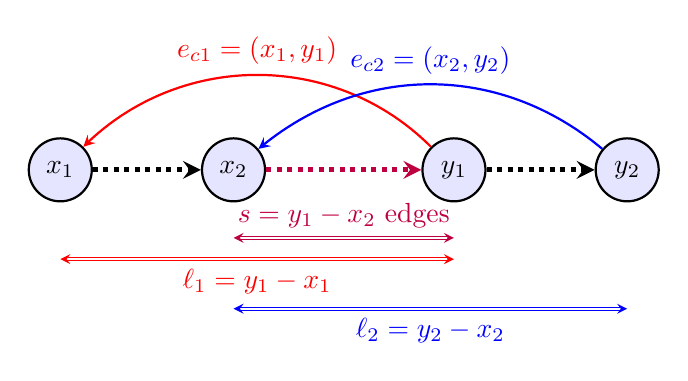
\begin{tikzpicture}[scale=0.9, >=stealth, main/.style={circle, draw=black, fill=blue!10, thick, inner sep=0pt, minimum size=8mm}]
		% Nodes
		\node[main] (x1) {$x_1$};
		\node[main] (x2) [right of=x1, node distance=2.2cm] {$x_2$};
		\node[main] (y1) [right of=x2, node distance=2.8cm] {$y_1$};
		\node[main] (y2) [right of=y1, node distance=2.2cm] {$y_2$};
		
		% Tree Edges
		\draw[dotted,line width=1.8pt, ->] (x1) -- node[above] {} (x2);
		\draw[dotted, line width=1.8pt, purple, ->] (x2) -- node[above, black] {} (y1);
		\draw[dotted,line width=1.8pt, ->] (y1) -- node[above] {} (y2);
		
		% Reverse Cycle Edges
		\draw[thick, red, ->] (y1) to[out=135, in=45] node[above, red] {$e_{c1} = (x_1, y_1)$} (x1);
		\draw[thick, blue, ->] (y2) to[out=140, in=40] node[above, blue] {$e_{c2} = (x_2, y_2)$} (x2);
		
		% Overlap and Length Braces
		\draw[style=double, <->, red] ([yshift=-8mm]x1.south) -- node[below, red] {$\ell_1 = y_1 - x_1$} ([yshift=-8mm]y1.south);
		\draw[style=double, <->, blue] ([yshift=-15mm]x2.south) -- node[below, blue] {$\ell_2 = y_2 - x_2$} ([yshift=-15mm]y2.south);
		\draw[style=double, <->, purple] ([yshift=-5mm]x2.south) -- node[above, purple] {$s = y_1 - x_2$ edges} ([yshift=-5mm]y1.south);
	\end{tikzpicture}
	\caption{Path graph $\mathcal{P}_n$ with two overlapping cycles sharing $s = |\mathcal{E}_{\text{cycle1}} \cap \mathcal{E}_{\text{cycle2}}| > 0$ tree edges.}
	\label{fig:ch_RA_dual_overlapping_cycles}
\end{figure}
\begin{theo}[Non-Overlapping Cycles]\label{nonoverlap}
For two completely non-overlapping cycles ($s = 0$), $D(0) = \frac{\ell_1 + \ell_2 + 2}{(\ell_1+1)(\ell_2+1)} = \frac{1}{\ell_1+1} + \frac{1}{\ell_2+1}$. Under a fixed total cycle edge budget $\ell_1 + \ell_2 = n-1$, $D(0)$ is uniquely minimized when the two non-overlapping cycles are equal in length ($\ell_1 = \ell_2 = \frac{n-1}{2}$ for odd $n$), yielding:
\begin{equation}\label{min_nonoverlap}
	D_{\min} = \begin{cases} \frac{4}{n+1}, & \text{for odd } n \\ \frac{4(n+1)}{n(n+2)}, & \text{for even } n \end{cases}
\end{equation}
\end{theo}

\begin{proof}
Define the continuous function $f(x) \coloneqq \frac{1}{x+1}$ for $x > -1$. Computing derivatives:
\begin{equation}
	f'(x) = -\frac{1}{(x+1)^2}, \quad f''(x) = \frac{2}{(x+1)^3} > 0 \quad \forall x > -1
\end{equation}
Since $f''(x) > 0$, $f(x)$ is strictly convex. By Jensen's Inequality \cite{perlman1974jensen}:
\begin{equation}\label{eq:ch_RA_jensen_proof}
	\frac{f(\ell_1) + f(\ell_2)}{2} \ge f\left( \frac{\ell_1 + \ell_2}{2} \right) \implies \frac{1}{\ell_1+1} + \frac{1}{\ell_2+1} \ge \frac{2}{\frac{\ell_1+\ell_2}{2} + 1} = \frac{4}{\ell_1 + \ell_2 + 2}
\end{equation}
where strict equality holds if and only if $\ell_1 = \ell_2$.

For a path graph on $n$ nodes, non-overlapping cycles span at most $n-1$ total edges ($\ell_1 + \ell_2 \le n-1$). Maximizing total length $\ell_1 + \ell_2 = n-1$ we have:
\begin{enumerate}
	\item \textbf{Odd $n$:} Setting $\ell_1 = \ell_2 = \frac{n-1}{2}$ gives $D_{\min} = \frac{4}{\frac{n-1}{2} + \frac{n-1}{2} + 2} = \frac{4}{n+1}$.
	\item \textbf{Even $n$:} Setting $\ell_1 = \frac{n}{2}$ and $\ell_2 = \frac{n}{2}-1$ gives:
	\begin{equation}
		D_{\min} = \frac{1}{\frac{n}{2}+1} + \frac{1}{\frac{n}{2}} = \frac{2}{n+2} + \frac{2}{n} = \frac{2n + 2(n+2)}{n(n+2)} = \frac{4(n+1)}{n(n+2)}
	\end{equation}
\end{enumerate}
This completes the proof.
\end{proof}
\begin{theo}[$\mathcal{H}_2$ Norm for Two Interacting Cycles]\label{ch_RA_theo2}
Let $\mathcal{P}_n$ be an $n$-node path graph of double integrators containing two interacting cycles of lengths $\ell_1$ and $\ell_2$ sharing $s \ge 0$ edges. The exact $\mathcal{H}_2$ norm of the reduced system $\Sigma$ is:
\begin{align}\label{two_cycle_norm}
	\|\Sigma\|_2^2 = \frac{1}{2\gamma} &\left[ 2\sigma_r^2(n-1) + (\sigma_q^2 + \sigma_r^2)(n - 3 + D) + \sigma_q^2 \frac{(n-1)(n+1)}{6} \right. \nonumber \\
	&\left. + \frac{\sigma_q^2}{d^2} \text{trace}\left( \letree^{-1} (c_1 t_1 t_1^T + c_2 t_1 t_2^T + c_3 t_2 t_1^T + c_4 t_2 t_2^T) \right) \right]
\end{align}
where $T = \begin{bmatrix} t_1 & t_2 \end{bmatrix} \in \mathbb{R}^{(n-1) \times 2}$, and scalar constants $d, D, c_1, c_2, c_3, c_4$ are defined as:
\begin{align}\label{eq:ch_RA_two_cycle_constants}
	d &\coloneqq (\ell_1+1)(\ell_2+1) - s^2, \quad D \coloneqq \frac{\ell_1 + \ell_2 + 2}{d} \nonumber \\
	c_1 &\coloneqq \ell_1(\ell_2+1)^2 - (\ell_2+2)s^2 - 2d(\ell_2+1), \quad c_4 \coloneqq \ell_2(\ell_1+1)^2 - (\ell_1+2)s^2 - 2d(\ell_1+1) \nonumber \\
	c_2 &= c_3 \coloneqq s(s^2 + 2d + 1 - \ell_1 \ell_2)
\end{align}
\end{theo}

\begin{proof}
Consider two cycles represented as, $T = \begin{bmatrix} t_1 & t_2 \end{bmatrix} \in \mathbb{R}^{(n-1) \times 2}$, where $t_1$ and $t_2$ are indicator vectors for Cycle 1 and Cycle 2. The matrix product $T^T T \in \mathbb{R}^{2 \times 2}$ is given by:
\begin{equation}\label{eq:ch_RA_TTT_2cycle}
	T^T T = \begin{bmatrix} t_1^T t_1 & t_1^T t_2 \\ t_2^T t_1 & t_2^T t_2 \end{bmatrix} = \begin{bmatrix} \ell_1 & s \\ s & \ell_2 \end{bmatrix}
\end{equation}

Observe that $I_2 + T^T T = \begin{bmatrix} \ell_1+1 & s \\ s & \ell_2+1 \end{bmatrix}$. Its determinant is $d = \det(I_2 + T^T T) = (\ell_1+1)(\ell_2+1) - s^2$. The inverse is thus given by:
\begin{equation}\label{eq:ch_RA_I_TTT_inv}
	(I_2 + T^T T)^{-1} = \frac{1}{d} \begin{bmatrix} \ell_2+1 & -s \\ -s & \ell_1+1 \end{bmatrix} \eqcolon \begin{bmatrix} a_1 & a_2 \\ a_3 & a_4 \end{bmatrix}
\end{equation}
where $a_1 = \frac{\ell_2+1}{d}$, $a_2 = a_3 = -\frac{s}{d}$, and $a_4 = \frac{\ell_1+1}{d}$.

Applying Woodbury's identity to $(R R^T)^{-1} = (I_{n-1} + T T^T)^{-1} = I_{n-1} - T (I_2 + T^T T)^{-1} T^T$:
\begin{align}\label{eq:ch_RA_RRT_inv_2cycle}
	\text{trace}\left((R R^T)^{-1}\right) &= \text{trace}(I_{n-1}) - \text{trace}\left( T (I_2 + T^T T)^{-1} T^T \right) \nonumber \\
	&= (n-1) - \text{trace}\left( (I_2 + T^T T)^{-1} T^T T \right) \nonumber \\
	&= (n-1) - \text{trace}\left( \frac{1}{d} \begin{bmatrix} \ell_2+1 & -s \\ -s & \ell_1+1 \end{bmatrix} \begin{bmatrix} \ell_1 & s \\ s & \ell_2 \end{bmatrix} \right) \nonumber \\
	&= (n-1) - \frac{(\ell_1(\ell_2+1) - s^2) + (\ell_2(\ell_1+1) - s^2)}{d} \nonumber \\
	&= (n-1) - \frac{2\ell_1 \ell_2 + \ell_1 + \ell_2 - 2s^2}{d} \nonumber \\
	&= n - 3 + \frac{\ell_1 + \ell_2 + 2}{d} = n - 3 + D
\end{align}
where $D = \frac{\ell_1 + \ell_2 + 2}{d}$.

Next, evaluate $(R R^T)^{-2} \letree^{-1} = \left[ I_{n-1} - T (I_2 + T^T T)^{-1} T^T \right]^2 \letree^{-1}$:
\begin{align}\label{eq:ch_RA_RRT_sq_2cycle}
	(R R^T)^{-2} \letree^{-1} &= \letree^{-1} - 2 T (I_2 + T^T T)^{-1} T^T \letree^{-1} + T (I_2 + T^T T)^{-1} T^T T (I_2 + T^T T)^{-1} T^T \letree^{-1} \nonumber \\
	&= \letree^{-1} + T \left[ (I_2 + T^T T)^{-1} T^T T (I_2 + T^T T)^{-1} - 2 (I_2 + T^T T)^{-1} \right] T^T \letree^{-1}
\end{align}

Defining matrix $B_{\text{mid}} \coloneqq (I_2 + T^T T)^{-1} T^T T (I_2 + T^T T)^{-1} = \begin{bmatrix} b_1 & b_2 \\ b_3 & b_4 \end{bmatrix}$ yields:
\begin{align}\label{eq:ch_RA_b_coefficients}
	b_1 &= \frac{\ell_1(\ell_2+1)^2 - (\ell_2+2)s^2}{d^2} \nonumber \\
	b_2 = b_3 &= \frac{s(s^2 + s - \ell_1 \ell_2)}{d^2} \nonumber \\
	b_4 &= \frac{\ell_2(\ell_1+1)^2 - (\ell_1+2)s^2}{d^2}
\end{align}
Defining $c_i \coloneqq d^2 (b_i - 2a_i)$ for $i \in \{1, 2, 3, 4\}$ gives the explicit expressions in \eqref{eq:ch_RA_two_cycle_constants}. Substituting $M_c = \sum_{i,j} c_{i,j} t_i t_j^T$ into the trace equation produces \eqref{two_cycle_norm}, thereby completing the proof.
\end{proof}

When process noise is zero ($\sigma_q = 0$), expression \eqref{two_cycle_norm} simplifies to:
\begin{equation}\label{eq:ch_RA_norm_edge_noise_only}
	\|\Sigma\|_{\sigma_q=0}^2 = \frac{\sigma_r^2}{2\gamma} \left[ 2(n-1) + n - 3 + D \right] = \frac{\sigma_r^2}{2\gamma} \left( 3n - 5 + D \right).
\end{equation}
Under edge noise alone, performance is governed solely by the scalar $D(s, \ell_1, \ell_2) \coloneqq \frac{\ell_1 + \ell_2 + 2}{(\ell_1+1)(\ell_2+1) - s^2}$. Minimizing $\|\Sigma\|_2^2$ is thus equivalent to minimizing $D(s, \ell_1, \ell_2)$.
\begin{comment}
\begin{theo}\label{overlap}
Given an undirected path graph of double integrators on $n$ nodes ($n>4$), suppose two interacting cycles of lengths $\ell_1$ and $\ell_2$ with $s$ shared edges between them results from the addition of two edges. Then, there exist $s>0$ for which the $D \le D_{\min}$, where, $D_{\min}$ is given in \eqref{min_nonoverlap}.
\end{theo}
\end{comment}
Having established that the optimal performance achievable with two non-overlapping cycles occurs when $\ell_1 = \ell_2 = \frac{n-1}{2}$ for odd $n$ (and $\ell_1 = \frac{n}{2}, \ell_2 = \frac{n}{2}-1$ for even $n$), a natural question arises: can introducing spatial overlap between these two cycles enhance $\mathcal{H}_2$ performance even further? The following result addresses this question by establishing exact bounds on the extent of edge overlap that guarantees superior disturbance rejection compared to the optimal non-overlapping baseline established above.
\begin{theo}\label{overlap}
Consider an undirected path graph of double integrators on $n$ nodes ($n > 4$) containing two interacting cycles of lengths $\ell_1$ and $\ell_2$ sharing $s \ge 0$ tree edges resulting from the addition of two cycle-closing edges. Let $D(s)$ denote the performance scalar:
\begin{equation}\label{eq:ch_RA_Ds_def}
	D(s) \coloneqq \frac{\ell_1 + \ell_2 + 2}{(\ell_1+1)(\ell_2+1) - s^2}.
\end{equation}
Furthermore, let the baseline non-overlapping configuration ($s = 0$) span the total edge budget $\ell_1 + \ell_2 = n-1$ such that:
\begin{equation}\label{eq:ch_RA_baseline_lengths}
	(\ell_1, \ell_2) = \begin{cases} \left(\frac{n-1}{2}, \frac{n-1}{2}\right), & \text{for odd } n, \\[6pt] \left(\frac{n}{2}, \frac{n}{2}-1\right), & \text{for even } n, \end{cases}
\end{equation}
which achieves the baseline minimum scalar:
\begin{equation}
	D_{\min} \coloneqq \begin{cases} \frac{4}{n+1}, & \text{for odd } n, \\[6pt] \frac{4(n+1)}{n(n+2)}, & \text{for even } n. \end{cases}
\end{equation}
Then, there exists a non-trivial edge overlap $s > 0$ achieved by expanding the cycle lengths beyond their baseline values \eqref{eq:ch_RA_baseline_lengths} such that $D(s) \le D_{\min}$. Specifically, performance improvement ($D(s) \le D_{\min}$) is guaranteed whenever the spatial overlap increments $k_1$ and $k_2$ (where $s = k_1 + k_2$) satisfy:
\begin{enumerate}
	\item \textbf{For odd $n$:}
	\begin{equation}\label{odd_minD}
		\frac{k_1^2 + k_2^2 + k_1 k_2}{k_1 + k_2} \le \frac{n+1}{4}.
	\end{equation}
	\item \textbf{For even $n$:}
	\begin{equation}\label{even_minD}
		\frac{k_1^2 + k_2^2 + k_1 k_2}{k_1 + k_2} - \frac{k_2}{k_1 + k_2} \le \frac{n^2}{4(n+1)}.
	\end{equation}
\end{enumerate}
\end{theo}
\begin{proof}
Case (1): When $n$ is odd. For non-overlapping case as base case as shown in Figure \ref{fig:ch_RA_base_case_odd_nodes}, we proved in Theorem \ref{nonoverlap} that $D_{\min}=\frac{4}{n+1}$. Now, Let $\ell_1=\frac{n-1}{2}+k_1$ and $\ell_2=\frac{n-1}{2}+k_2$ such that $s=k_1+k_2$ as shown in Figure \ref{fig:ch_RA_overlap_case_odd_nodes}. Thus,
\small
\begin{equation}
	D=\frac{n+1+k_1+k_2}{\frac{(n+1)^2}{4}+(k_1+k_2)\frac{n+1}{2}-k_1^2-k_2^2-k_1k_2}
\end{equation}
\normalsize
\begin{figure}[htbp]
	\centering
	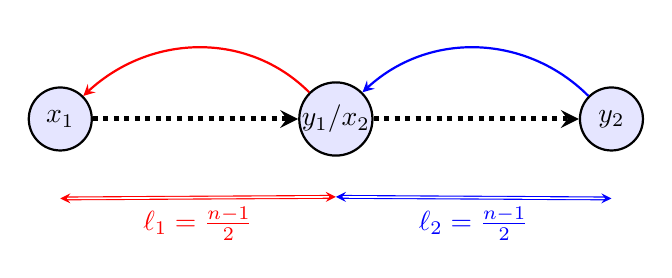
\begin{tikzpicture}[scale=0.85, >=stealth, main/.style={circle, draw=black, fill=blue!10, thick, inner sep=0pt, minimum size=8mm}]
		% Nodes
		\node[main] (x1) {$x_1$};
		\node[main] (y1x2) [right of=x1, node distance=3.5cm] {$y_1$/$x_2$};
		\node[main] (y2) [right of=y1x2, node distance=3.5cm] {$y_2$};
		
		% Spanning Tree Edges
		\draw[dotted,line width=1.8pt, ->] (x1) -- node[above] {} (y1x2);
		\draw[dotted,line width=1.8pt, ->] (y1x2) -- node[above] {} (y2);
		
		% Reverse Cycle Edges
		\draw[thick, red, ->] (y1x2) to[out=135, in=45] node[above, red] {} (x1);
		\draw[thick, blue, ->] (y2) to[out=135, in=45] node[above, blue] {} (y1x2);
		
		% Base Length Braces
		\draw[style=double, <->, red] ([yshift=-7mm]x1.south) -- node[below, red] {$\ell_1 = \frac{n-1}{2}$} ([yshift=-6mm]y1x2.south);
		\draw[style=double, <->, blue] ([yshift=-6mm]y1x2.south) -- node[below, blue] {$\ell_2 = \frac{n-1}{2}$} ([yshift=-7mm]y2.south);
	\end{tikzpicture}
	\caption{Optimal non-overlapping configuration ($s = 0$) for odd $n$, where the cycles meet at node $y_1 = x_2$ without sharing tree edges.}
	\label{fig:ch_RA_base_case_odd_nodes}
\end{figure}
\begin{figure}[htbp]
	\centering
	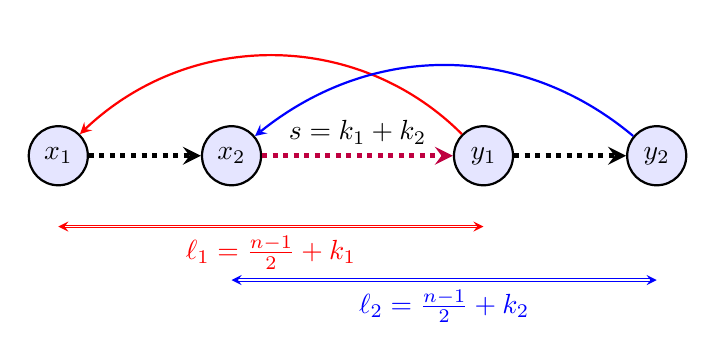
\begin{tikzpicture}[scale=0.85, >=stealth, main/.style={circle, draw=black, fill=blue!10, thick, inner sep=0pt, minimum size=7.5mm}]
		% Nodes
		\node[main] (x1) {$x_1$};
		\node[main] (x2) [right of=x1, node distance=2.2cm] {$x_2$};
		\node[main] (y1) [right of=x2, node distance=3.2cm] {$y_1$};
		\node[main] (y2) [right of=y1, node distance=2.2cm] {$y_2$};
		
		% Spanning Tree Edges
		\draw[dotted,line width=1.8pt, ->] (x1) -- node[above] {} (x2);
		\draw[dotted, line width=1.8pt, purple, ->] (x2) -- node[above, black] {$s = k_1 + k_2$} (y1);
		\draw[dotted,line width=1.8pt, ->] (y1) -- node[above] {} (y2);
		
		% Reverse Cycle Edges
		\draw[thick, red, ->] (y1) to[out=135, in=45] node[above, red] {} (x1);
		\draw[thick, blue, ->] (y2) to[out=140, in=40] node[above, blue] {} (x2);
		
		% Overlap and Expanded Length Braces
		\draw[style=double, <->, red] ([yshift=-6mm]x1.south) -- node[below, red] {$\ell_1 = \frac{n-1}{2} + k_1$} ([yshift=-6mm]y1.south);
		\draw[style=double, <->, blue] ([yshift=-14mm]x2.south) -- node[below, blue] {$\ell_2 = \frac{n-1}{2} + k_2$} ([yshift=-14mm]y2.south);
		%\draw[style=double, <->, purple] ([yshift=-6mm]x2.south) -- node[above, purple] {$s = k_1 + k_2$} ([yshift=-6mm]y1.south);
	\end{tikzpicture}
	\caption{Overlapping configuration showing cycle expansions by $k_1$ and $k_2$ resulting in $s = k_1 + k_2$ shared edges.}
	\label{fig:ch_RA_overlap_case_odd_nodes}
\end{figure}
To minimize it further, $D-D_{\min} \le 0$ needs to be satisfied.
On imposing this requirement, we get 
\begin{equation}
	\frac{k_1^2+k_2^2+k_1k_2}{k_1+k_2} \le \frac{n+1}{4}
\end{equation}
Case 1(a): If $k_1=0$ and $k_2=k$ such that $s=k$, we have
\begin{equation}\label{eq:ch_RA_one_edgeoverlap}
	k \le \frac{n+1}{4}
\end{equation}
Because of symmetry of inequality with respect to $k_1$ and $k_2$, same condition occurs if $k_1=k$ and $k_2=0$.

Case 1(b):If $k_1=k_2=k$ such that $s=2k$, then we have
\begin{equation}\label{eq:ch_RA_equal_edgeoverlap}
	k \le \frac{n+1}{6}
\end{equation}
Case (2): When $n$ is even. Let $\ell_1=\frac{n}{2}+k_1$ and $\ell_2=\frac{n}{2}+k_2-1$, with $s=k_1+k_2$. Thus, we have
\small
\begin{equation*}
	D=\frac{n+1+k_1+k_2}{\frac{n^2}{4}+(k_1+k_2+1)\frac{n}{2}+k_2-k_1^2-k_2^2-k_1k_2}.
\end{equation*}
\normalsize
For base case when $n$ is even, $D_{\min}=\frac{4(n+1)}{n(n+2)}$. To minimize it further, $D-D_{\min} \le 0$ needs to be satisfied.
On imposing this, we get 
\begin{equation}
	\frac{k_1^2+k_2^2+k_1k_2}{k_1+k_2}-\frac{k_2}{k_1+k_2} \le \frac{n^2}{4(n+1)}.
\end{equation}
Case 2(a): If $k_1=0$ and $k_2=k$ such that $s=k$, we have
\begin{equation}
	k \le \frac{n^2}{4(n+1)}+1.
\end{equation}

Case 2(b): If $k_2=0$ and $k_1=k$ such that $s=k$, then it follows that
\begin{equation}
	k \le \frac{n^2}{4(n+1)}.
\end{equation}
Case 2(c): If $k_1=k_2=k$ such that $s=2k$, then we have
\begin{equation}
	k \le \frac{1}{6}\left[n+1+\frac{1}{n+1}\right].
\end{equation}
In all the above cases, the upper bound on $k$ is greater than or equal to 1 for $n>4$, this completes the proof.    
\end{proof}
\begin{remark}
Theorem \ref{overlap} indicates that some amount of overlap is always desirable for an improved performance with respect to $\mathcal{H}_2$ metric in presence of two cycles in a graph.
\end{remark}
\begin{remark}
Though the present analysis was done for a network of double integrators, the same analysis is valid for the case of single integrators, under assumption that $\sigma_q=\sigma_r=1$. However, note that the analysis for double integrator is done under zero node noise, whereas it is equivalent to the single integrator case under influence of both kinds of noises, as in \cite{zelazo2013performance}.
\end{remark}

\section{Numerical Validation and Discussions}\label{sec:ch_RA_simulations}

To validate the theoretical bounds derived in Section \ref{sec:ch_RA_CycleAnalysis},extensive numerical simulations were conducted on a 23-node path graph ($\mathcal{P}_{23}$, $n = 23$) consisting of consensus-seeking double-integrator agents under velocity coupling gain $\gamma = 1$. The baseline non-overlapping configuration is established at the theoretical optimum given by Theorem \ref{nonoverlap} for odd $n$: Cycle~1 and Cycle~2 are assigned identical base length $\ell_1=\ell_2=11$, meeting at the central node $y_1 = x_2 = 12$ with zero edge overlap ($s=0$) and subject to process and measurement noise.

\begin{figure}[ht!]
	\centering
	\begin{subfigure}[b]{0.8\textwidth}
		\centering
		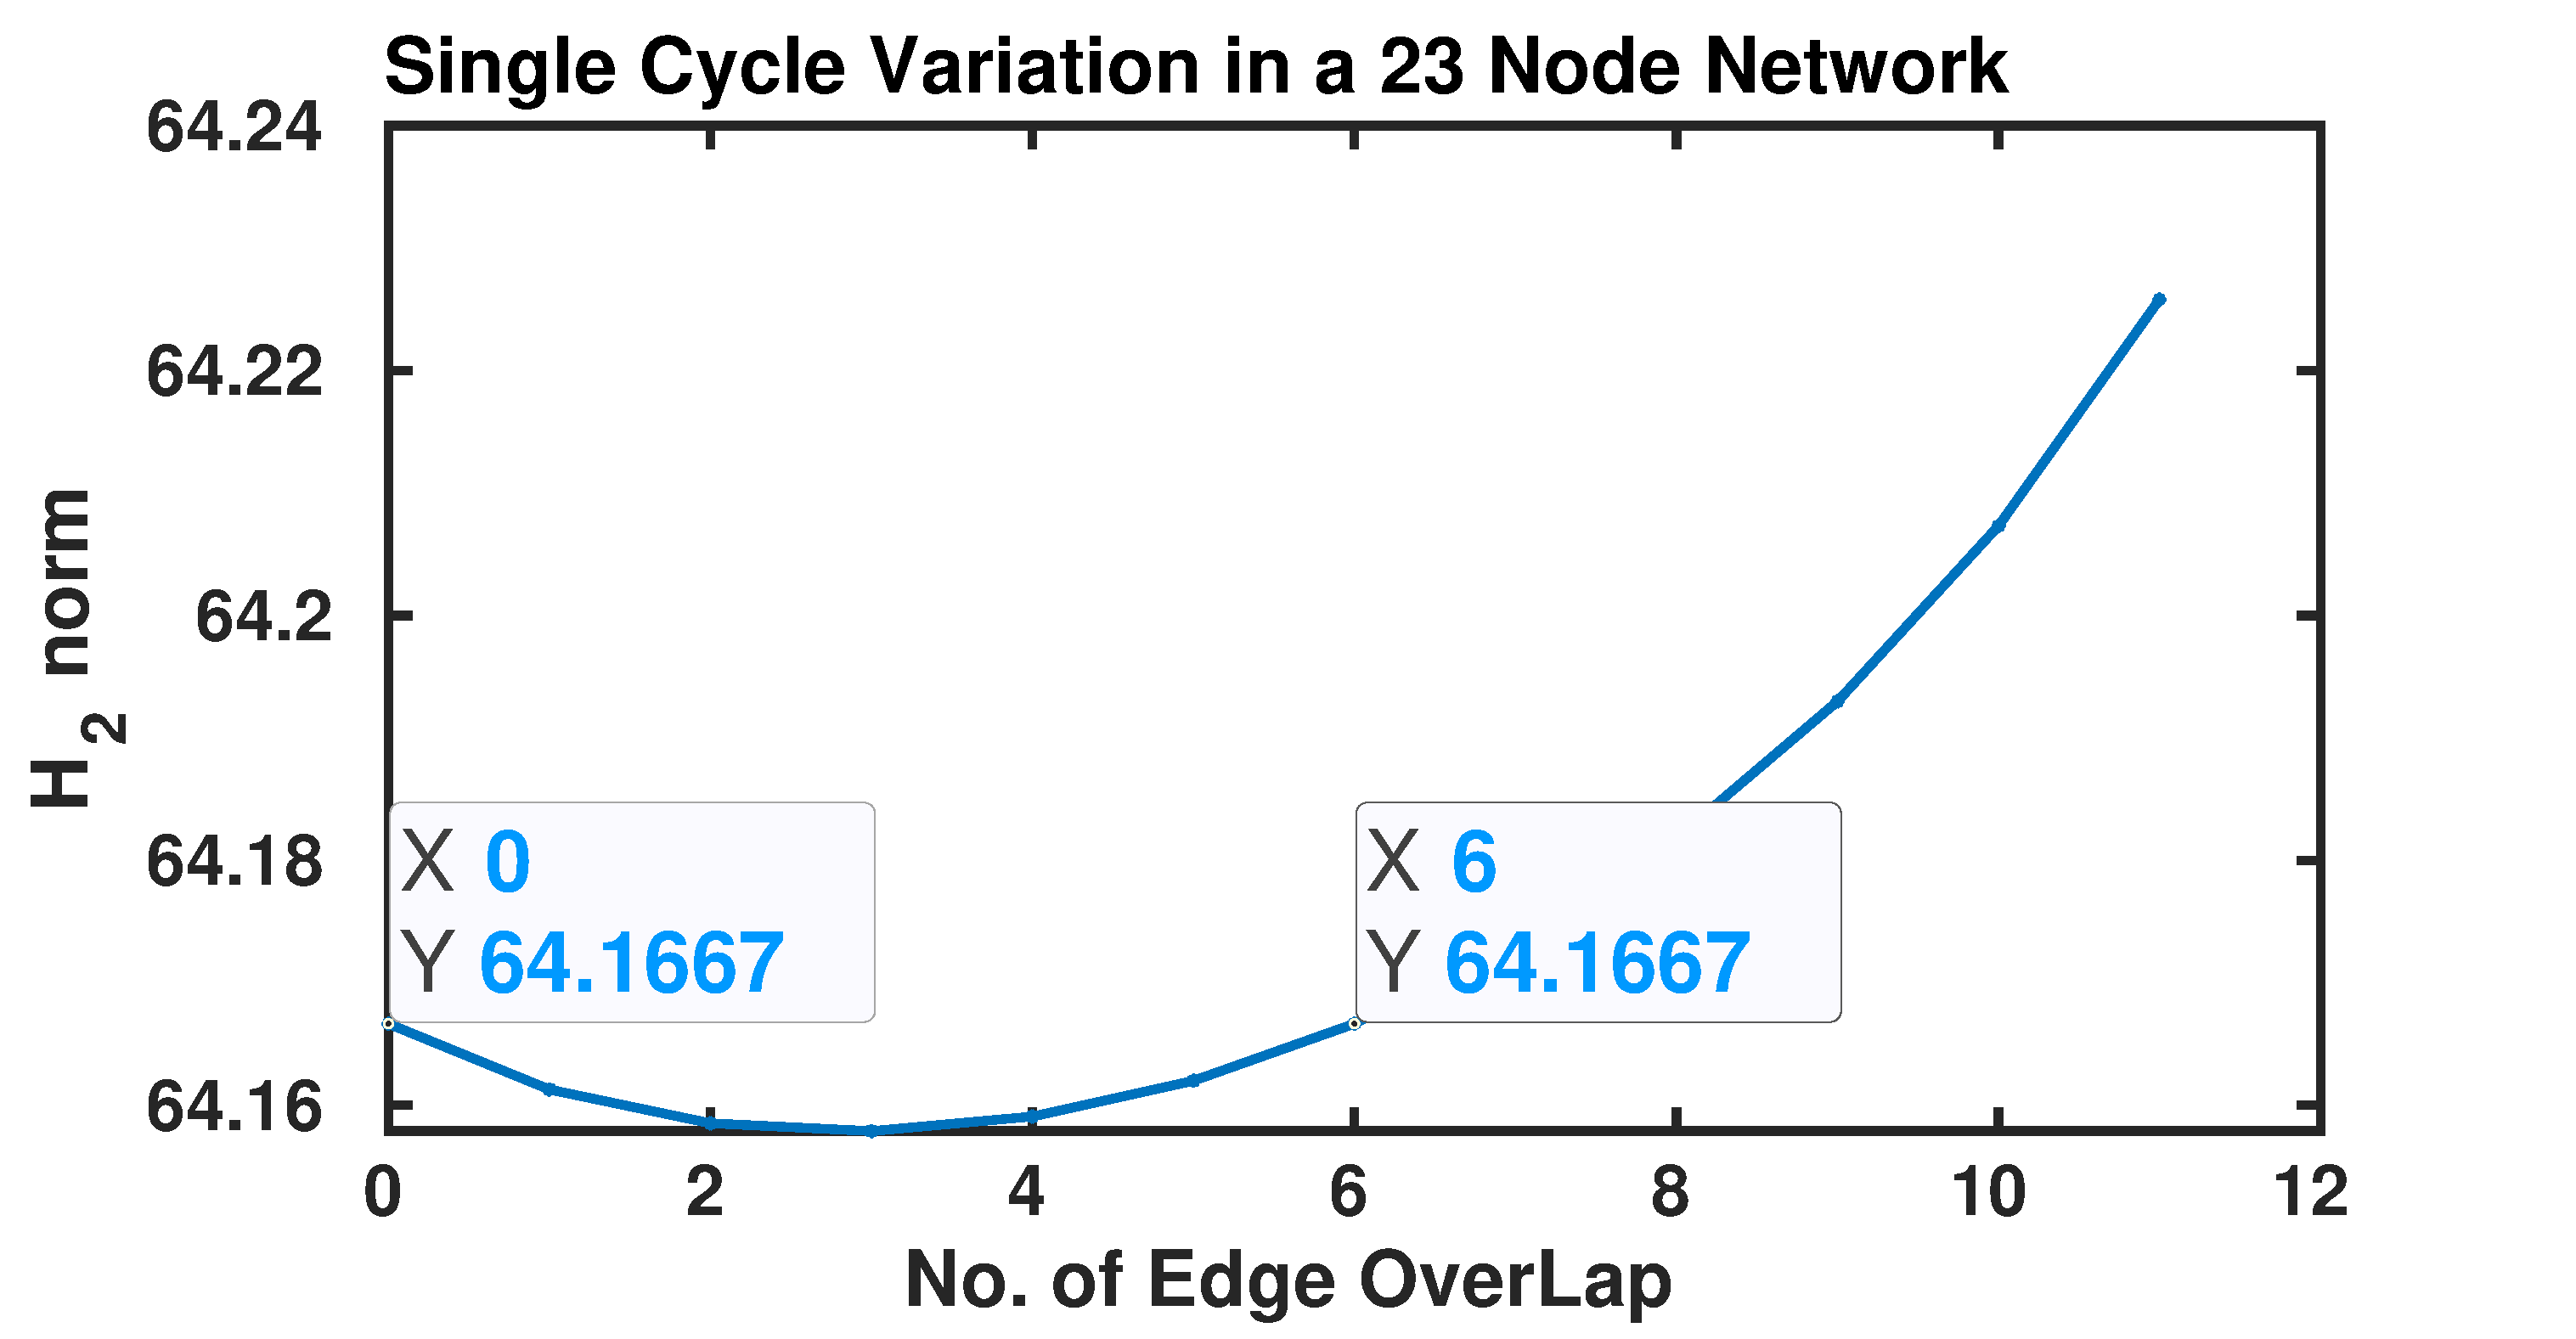
\includegraphics[width=\textwidth, keepaspectratio]{4_Images/Single_Cycle_Variation_23Nodes.eps}
		\caption{Single-cycle length increases by $k$ ($s = k$). Performance improves for $k \le \frac{23+1}{4} = 6$.}
		\label{fig:Single_Cycle_Variation_23Nodes}
	\end{subfigure}
	
	\vspace{1em}
	
	\begin{subfigure}[b]{0.8\textwidth}
		\centering
		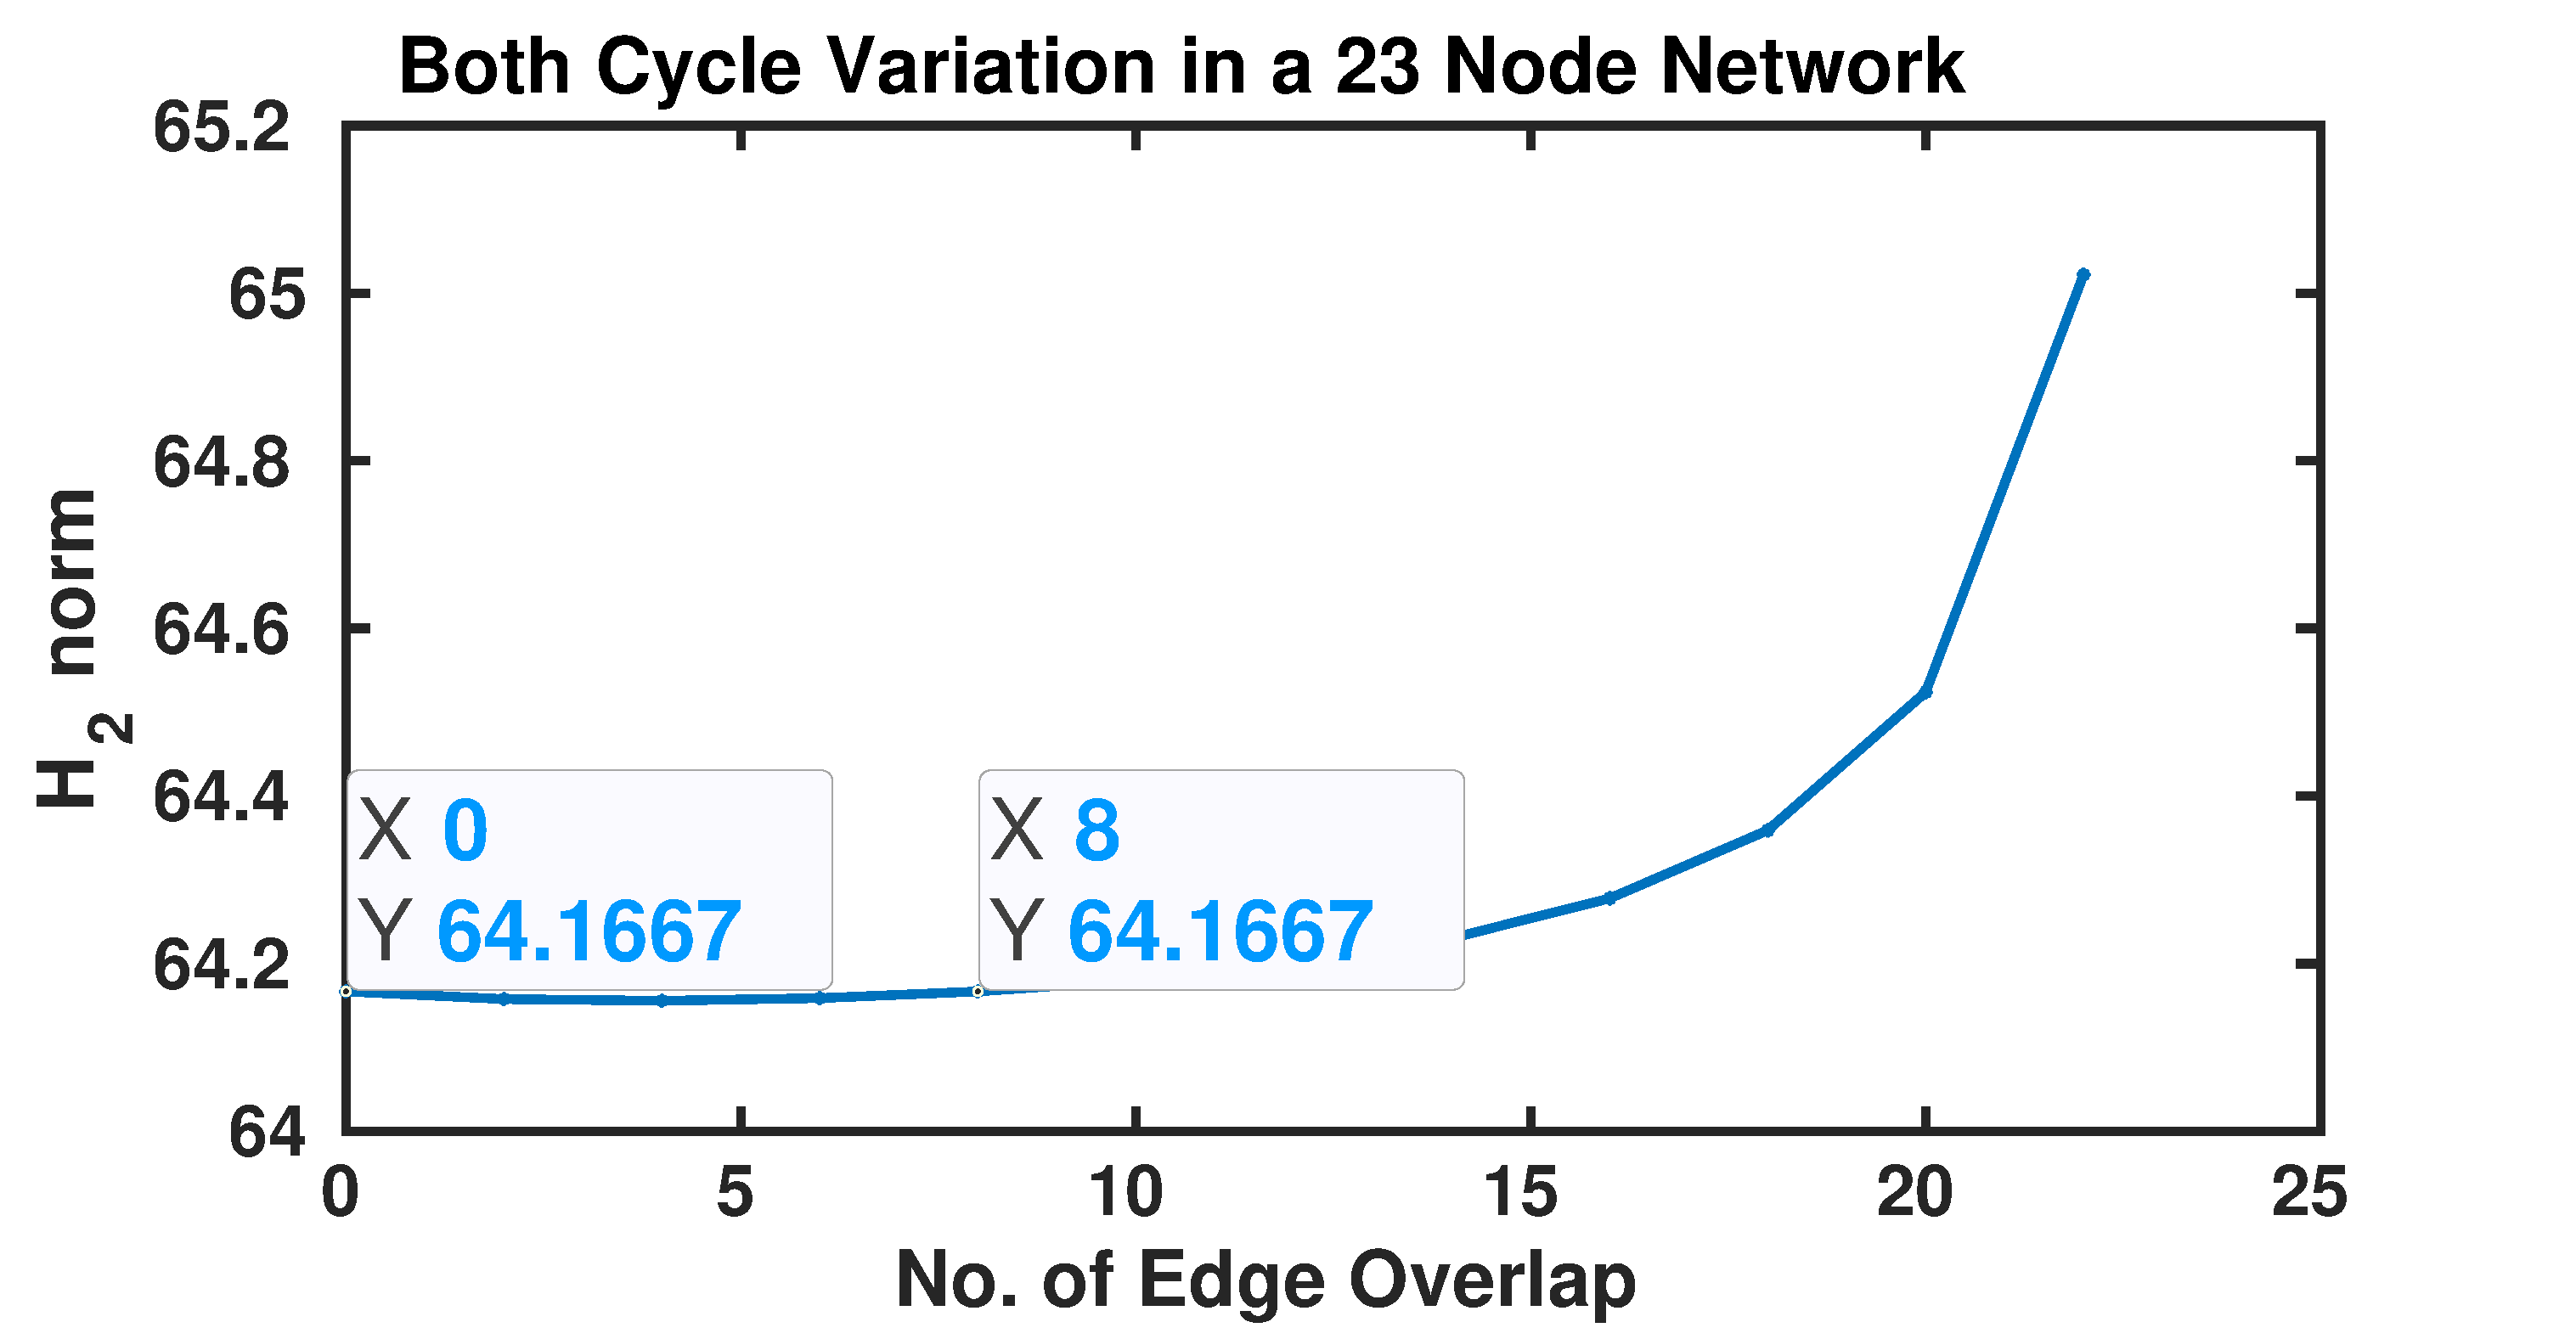
\includegraphics[width=\textwidth, keepaspectratio]{4_Images/Both_Cycle_Variation_23Nodes.eps}
		\caption{Both cycles' length increase by $k$ ($s = 2k$). Performance improves for $k \le \frac{23+1}{6} = 4$.}
		\label{fig:Both_Cycle_Variation_23Nodes}
	\end{subfigure}
	\caption{$\mathcal{H}_2$ norm variation as a function of edge overlap, $s$, between two cycles under measurement noise}
	\label{fig:withedgenoise}
\end{figure}

Figures \ref{fig:Single_Cycle_Variation_23Nodes} and \ref{fig:Both_Cycle_Variation_23Nodes} depict the variation of the system $\mathcal{H}_2$ norm $\|\Sigma\|_2^2$ under pure edge measurement noise ($\sigma_r^2 = 1, \sigma_q^2 = 0$) as a function of the spatial overlap increment $k$. 

In Figure~\ref{fig:Single_Cycle_Variation_23Nodes}, Cycle~1 is expanded by $k$ edges while keeping Cycle~2 fixed at its base length $\ell_2 = 11$, resulting in a direct spatial overlap $s = k$. As predicted by Case~1 of Theorem~\ref{overlap}, introducing edge overlap initially causes the system norm $\|\Sigma\|_2^2$ to decrease monotonically below the non-overlapping baseline $D_{\min}$. The performance metric achieves its global minimum at $k = 6$ ($s = 6$ shared edges), beyond which additional expansion causes $\|\Sigma\|_2^2$ to increase. This matches the analytical upper bound $k_{\max} = \frac{n+1}{4} = \frac{24}{4} = 6$ derived in \eqref{eq:ch_RA_one_edgeoverlap}.


Figure~\ref{fig:Both_Cycle_Variation_23Nodes} illustrates the symmetric dual-cycle expansion scenario, where both cycles are simultaneously expanded by $k$ edges ($\ell_1' = \ell_2' = 11 + k$), generating a mutual overlap $s = 2k$. In strict agreement with Case~2 of Theorem~\ref{overlap}, the $\mathcal{H}_2$ norm improves continuously until $k$ reaches $k_{\max} = \frac{n+1}{6} = \frac{24}{6} = 4$, which corresponds to an optimal shared region of $s = 2(4) = 8$ edges as derived in \eqref{eq:ch_RA_equal_edgeoverlap}. Beyond $k > 4$, excessive structural overlap creates redundant feedback channels that amplify measurement noise propagation, deteriorating overall network performance.

These results validate a fundamental design insight: \textbf{completely non-overlapping loops ($s = 0$) are suboptimal}. A certain degree of structural overlap acts as an algebraic dampener, creating parallel relative-state feedback channels that suppress transient noise energy without overloading the network.

\begin{figure}[ht!]
	\centering
	\begin{subfigure}[b]{0.8\textwidth}
		\centering
		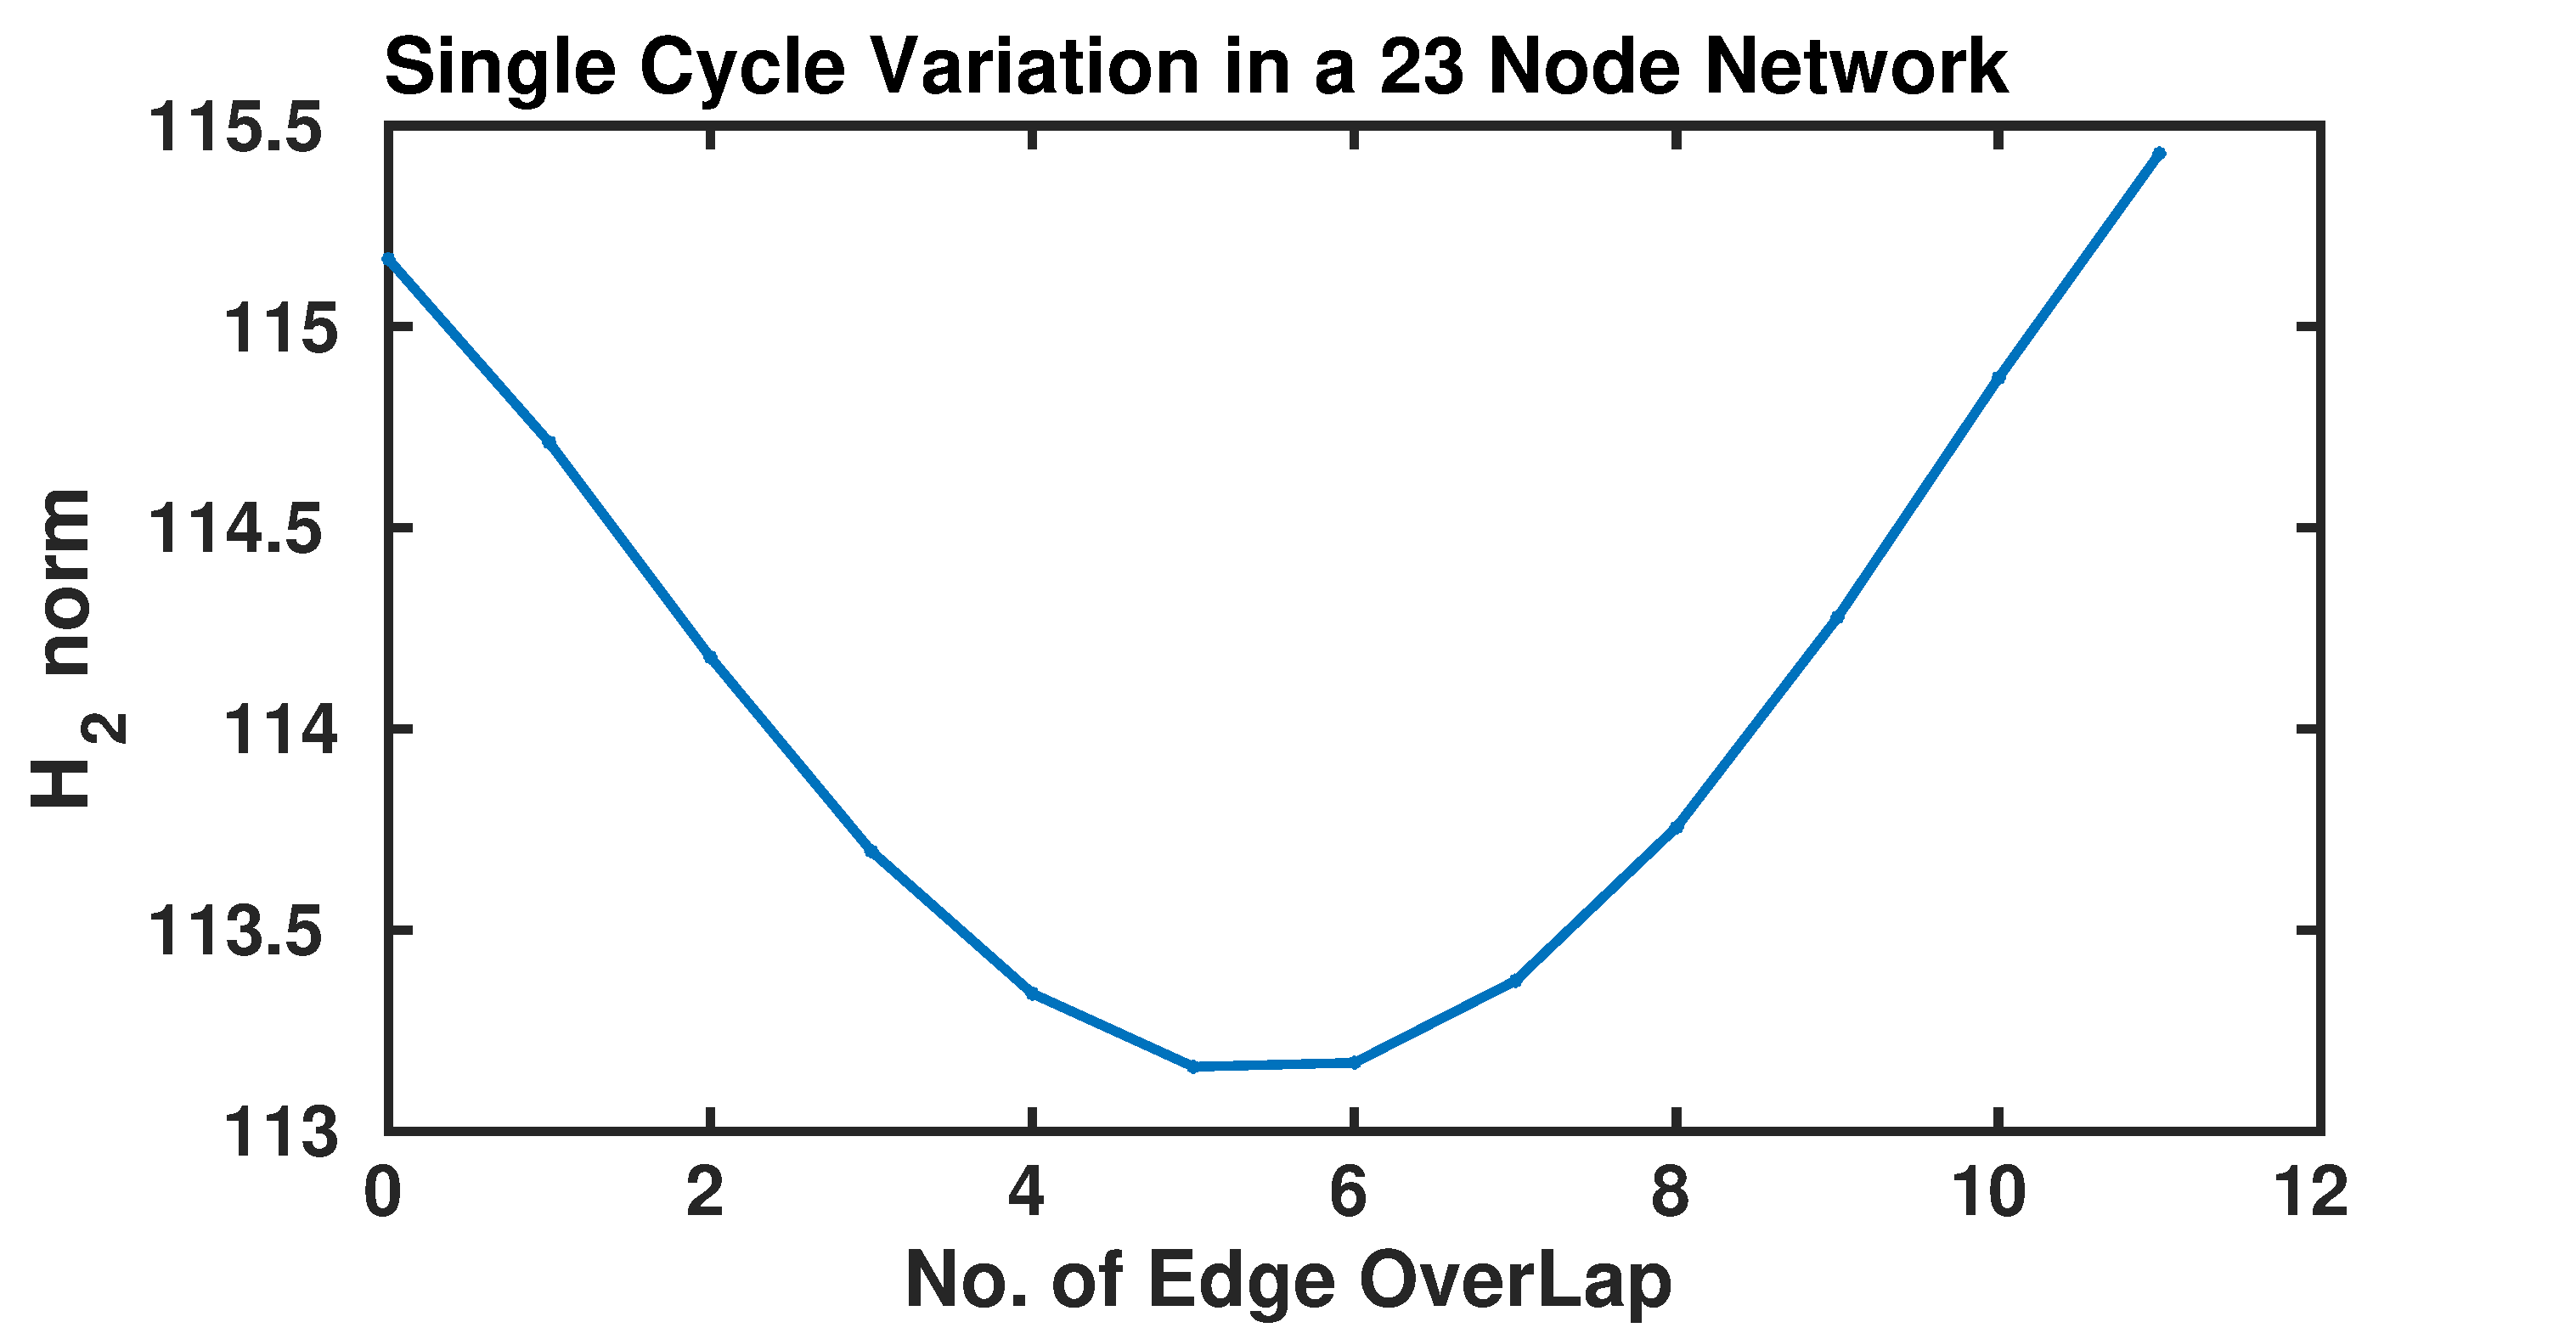
\includegraphics[width=\textwidth, keepaspectratio]{4_Images/Single_Cycle_Variation_23Nodes_BothNoise.eps}
		\caption{Single-cycle length increases under combined noise ($\sigma_q^2 = 1, \sigma_r^2 = 1$).}
		\label{fig:Single_BothNoise}
	\end{subfigure}
	
	\vspace{1em}
	
	\begin{subfigure}[b]{0.8\textwidth}
		\centering
		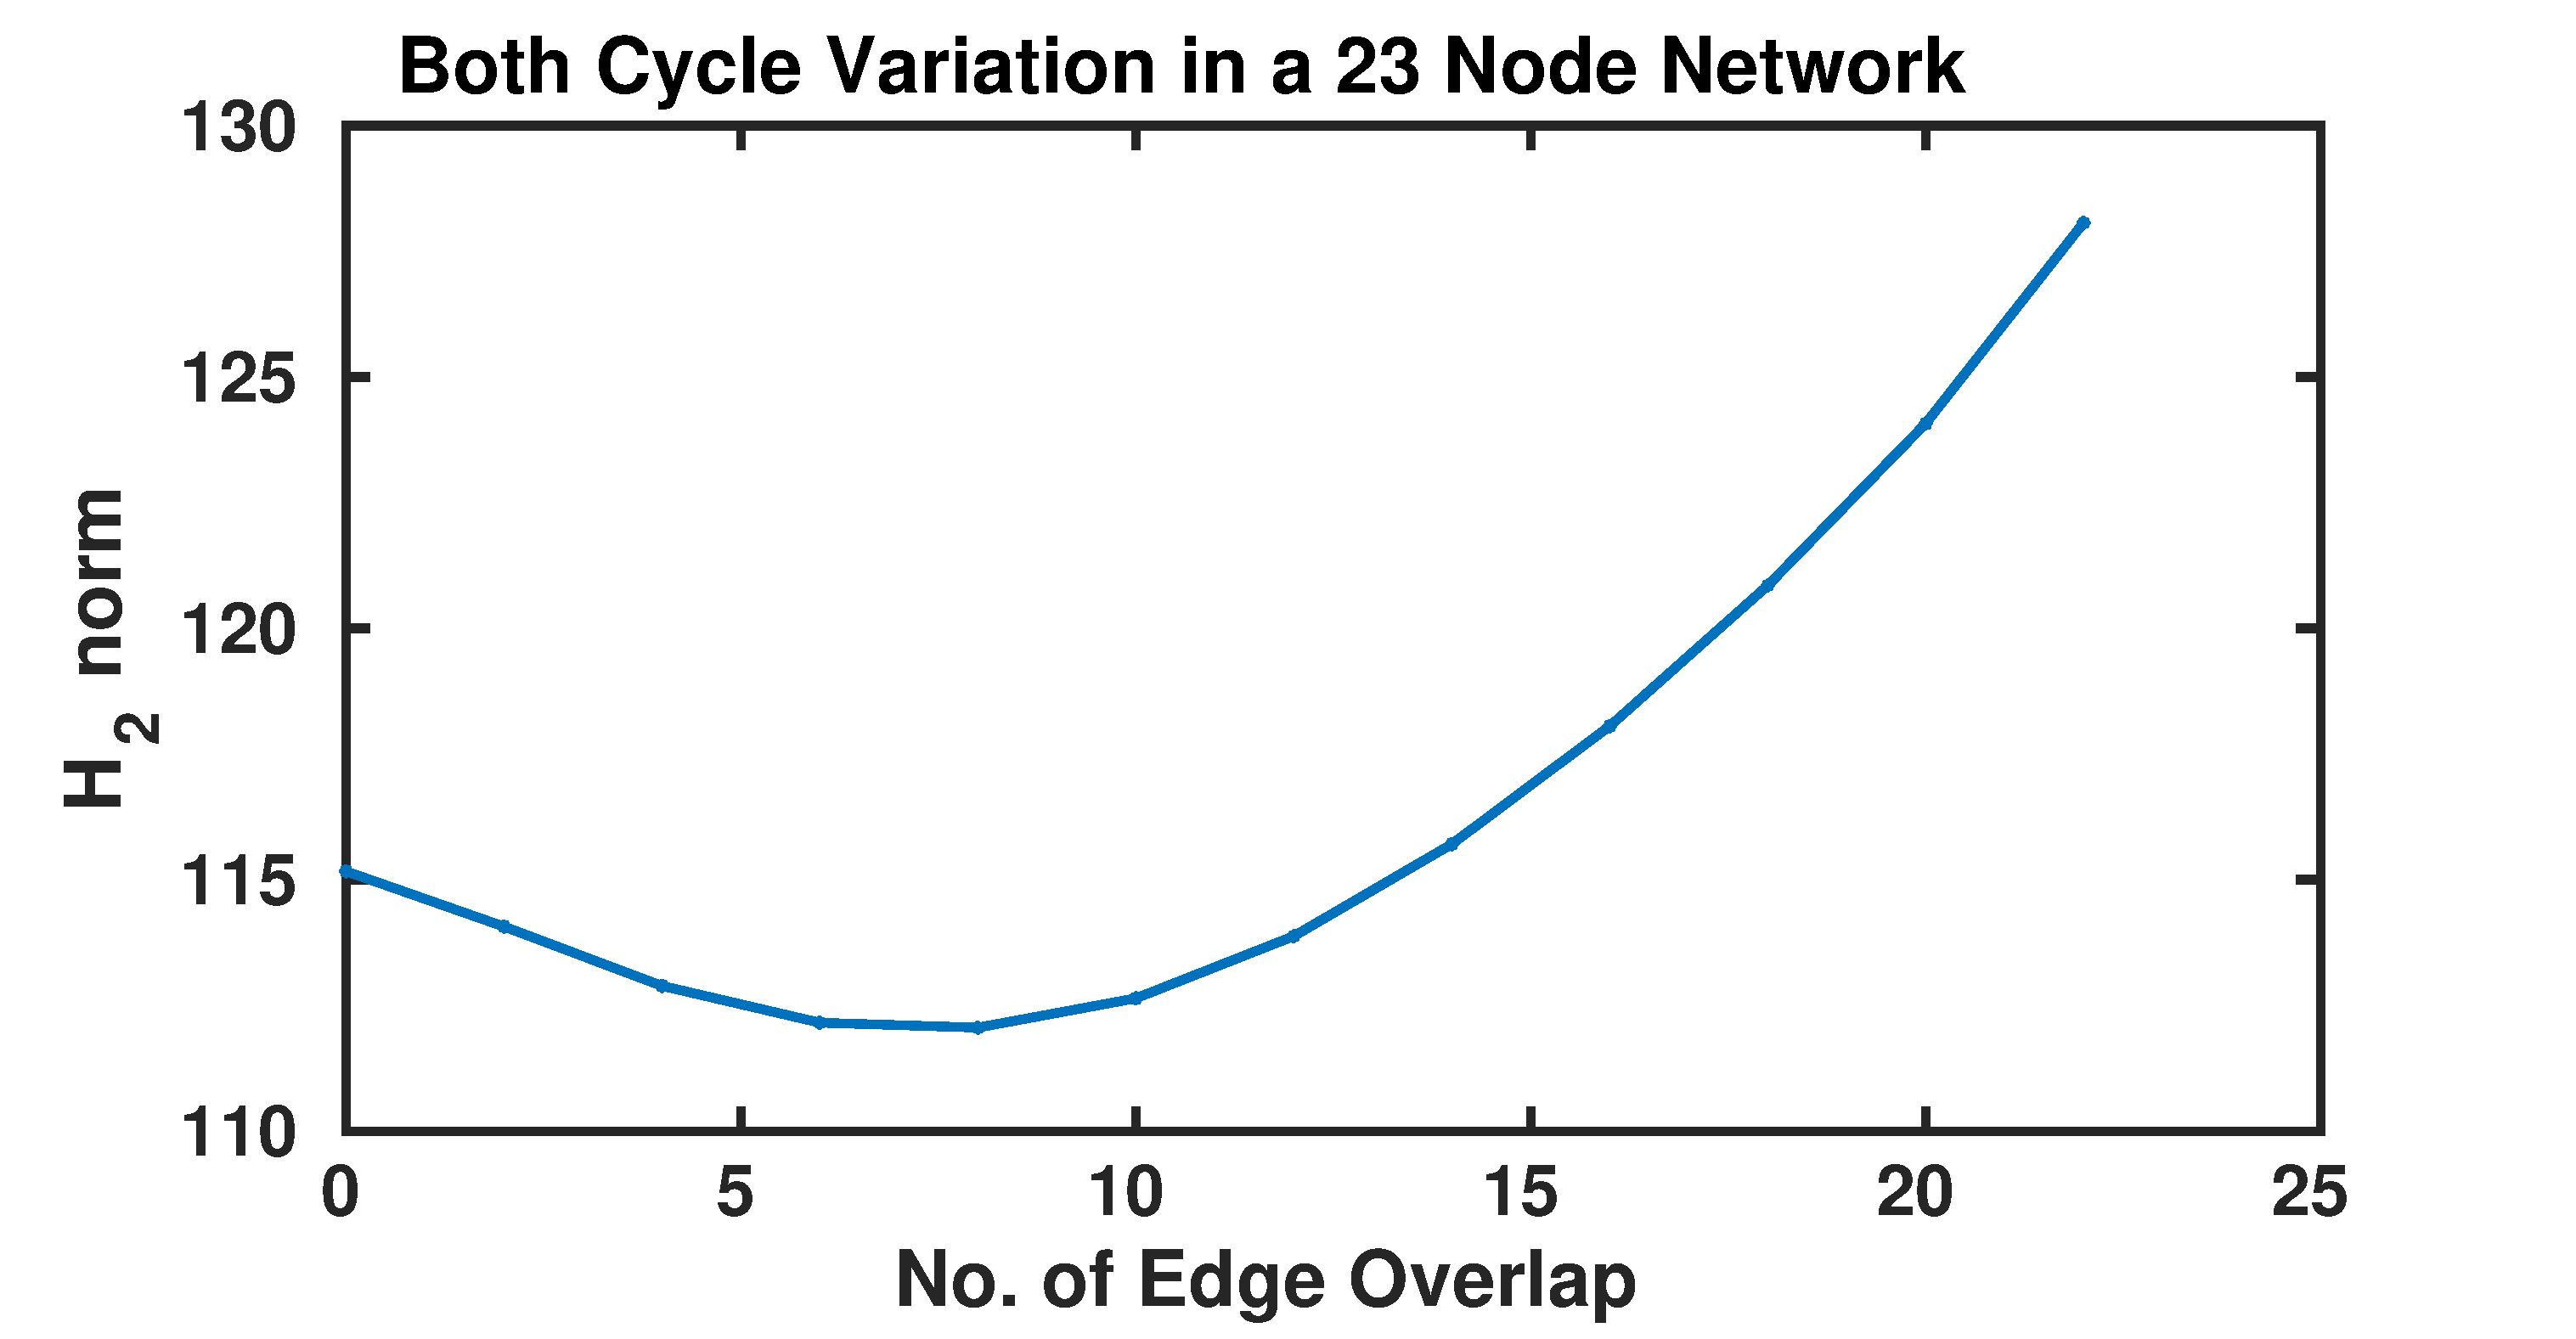
\includegraphics[width=\textwidth, keepaspectratio]{4_Images/Both_Cycle_Variation_23Nodes_BothNoise.eps}
		\caption{Both cycles' lengths increase under combined noise ($\sigma_q^2 = 1, \sigma_r^2 = 1$).}
		\label{fig:Both_BothNoise}
	\end{subfigure}
	\caption{$\mathcal{H}_2$ norm variation with two cycles under combined process and measurement noise.}
	\label{fig:withbothnoise}
\end{figure}

In practical deployments, multi-agent networks operate under simultaneous external process disturbances acting on agent acceleration dynamics ($\sigma_q^2 > 0$) and sensor measurement noise along communication links ($\sigma_r^2 > 0$). Figures~\ref{fig:Single_BothNoise} and \ref{fig:Both_BothNoise} evaluate the $\mathcal{H}_2$ norm under equal process and measurement noise power ($\sigma_q^2 = 1, \sigma_r^2 = 1$).

As observed in Figures~\ref{fig:Single_BothNoise} and \ref{fig:Both_BothNoise}, the addition of process noise scales the overall energy baseline of $\|\Sigma\|_2^2$ due to the persistent excitation of physical velocity states.

Specifically, moderate spatial overlap continues to yield superior disturbance rejection compared to the non-overlapping baseline $s = 0$. The minimum norm regions align closely with the analytical bounds established under pure edge noise, confirming that the optimal overlap bounds derived in Theorem~\ref{overlap} remain robust against process noises.

To validate Theorem~\ref{thm:ch_RA_single_cycle_location}, we analyze the sensitivity of $\|\Sigma\|_2^2$ to the spatial placement of cycle centers across the physical path graph. Figure~\ref{fig:Position_dependence} tracks the $\mathcal{H}_2$ norm across four distinct topological loop-triplet configurations ($\{\ell_1, \ell_2, s\}$) as their spatial anchoring indices are systematically shifted from the boundary nodes toward the graph interior.

The numerical results in Figure~\ref{fig:Position_dependence} demonstrate two critical phenomena:
\begin{enumerate}
	\item \textbf{Monotonic Centering Minimization:} For every tested loop geometry, shifting the cycle anchors closer to the network spatial center $n_c^* = \frac{23+1}{2} = 12$ produces a smooth, monotonic reduction in $\|\Sigma\|_2^2$. Trajectories positioned at the geographic boundaries (near node $1$ or node $23$) exhibit significantly higher noise amplification.
	\item \textbf{Hierarchy of Topological Configurations:} Across all spatial locations, configurations with non-zero edge overlap ($s > 0$) consistently achieve lower $\mathcal{H}_2$ norms than non-overlapping structures ($s = 0$). Specifically, the overlapping configurations $\{\ell_1=3, \ell_2=1, s=1\}$ and $\{\ell_1=4, \ell_2=1, s=1\}$ outperform the non-overlapping baseline $\{\ell_1=1, \ell_2=1, s=0\}$ across every spatial index.
\end{enumerate}

These findings confirm Theorem~\ref{thm:ch_RA_single_cycle_location} and provide some guidelines towards network design for achieving second-order consensus: optimal disturbance rejection requires both spatial centering of feedback loops relative to the graph midpoint and partial structural overlap between adjacent cycles.

\begin{figure}[ht!]
	\centering
	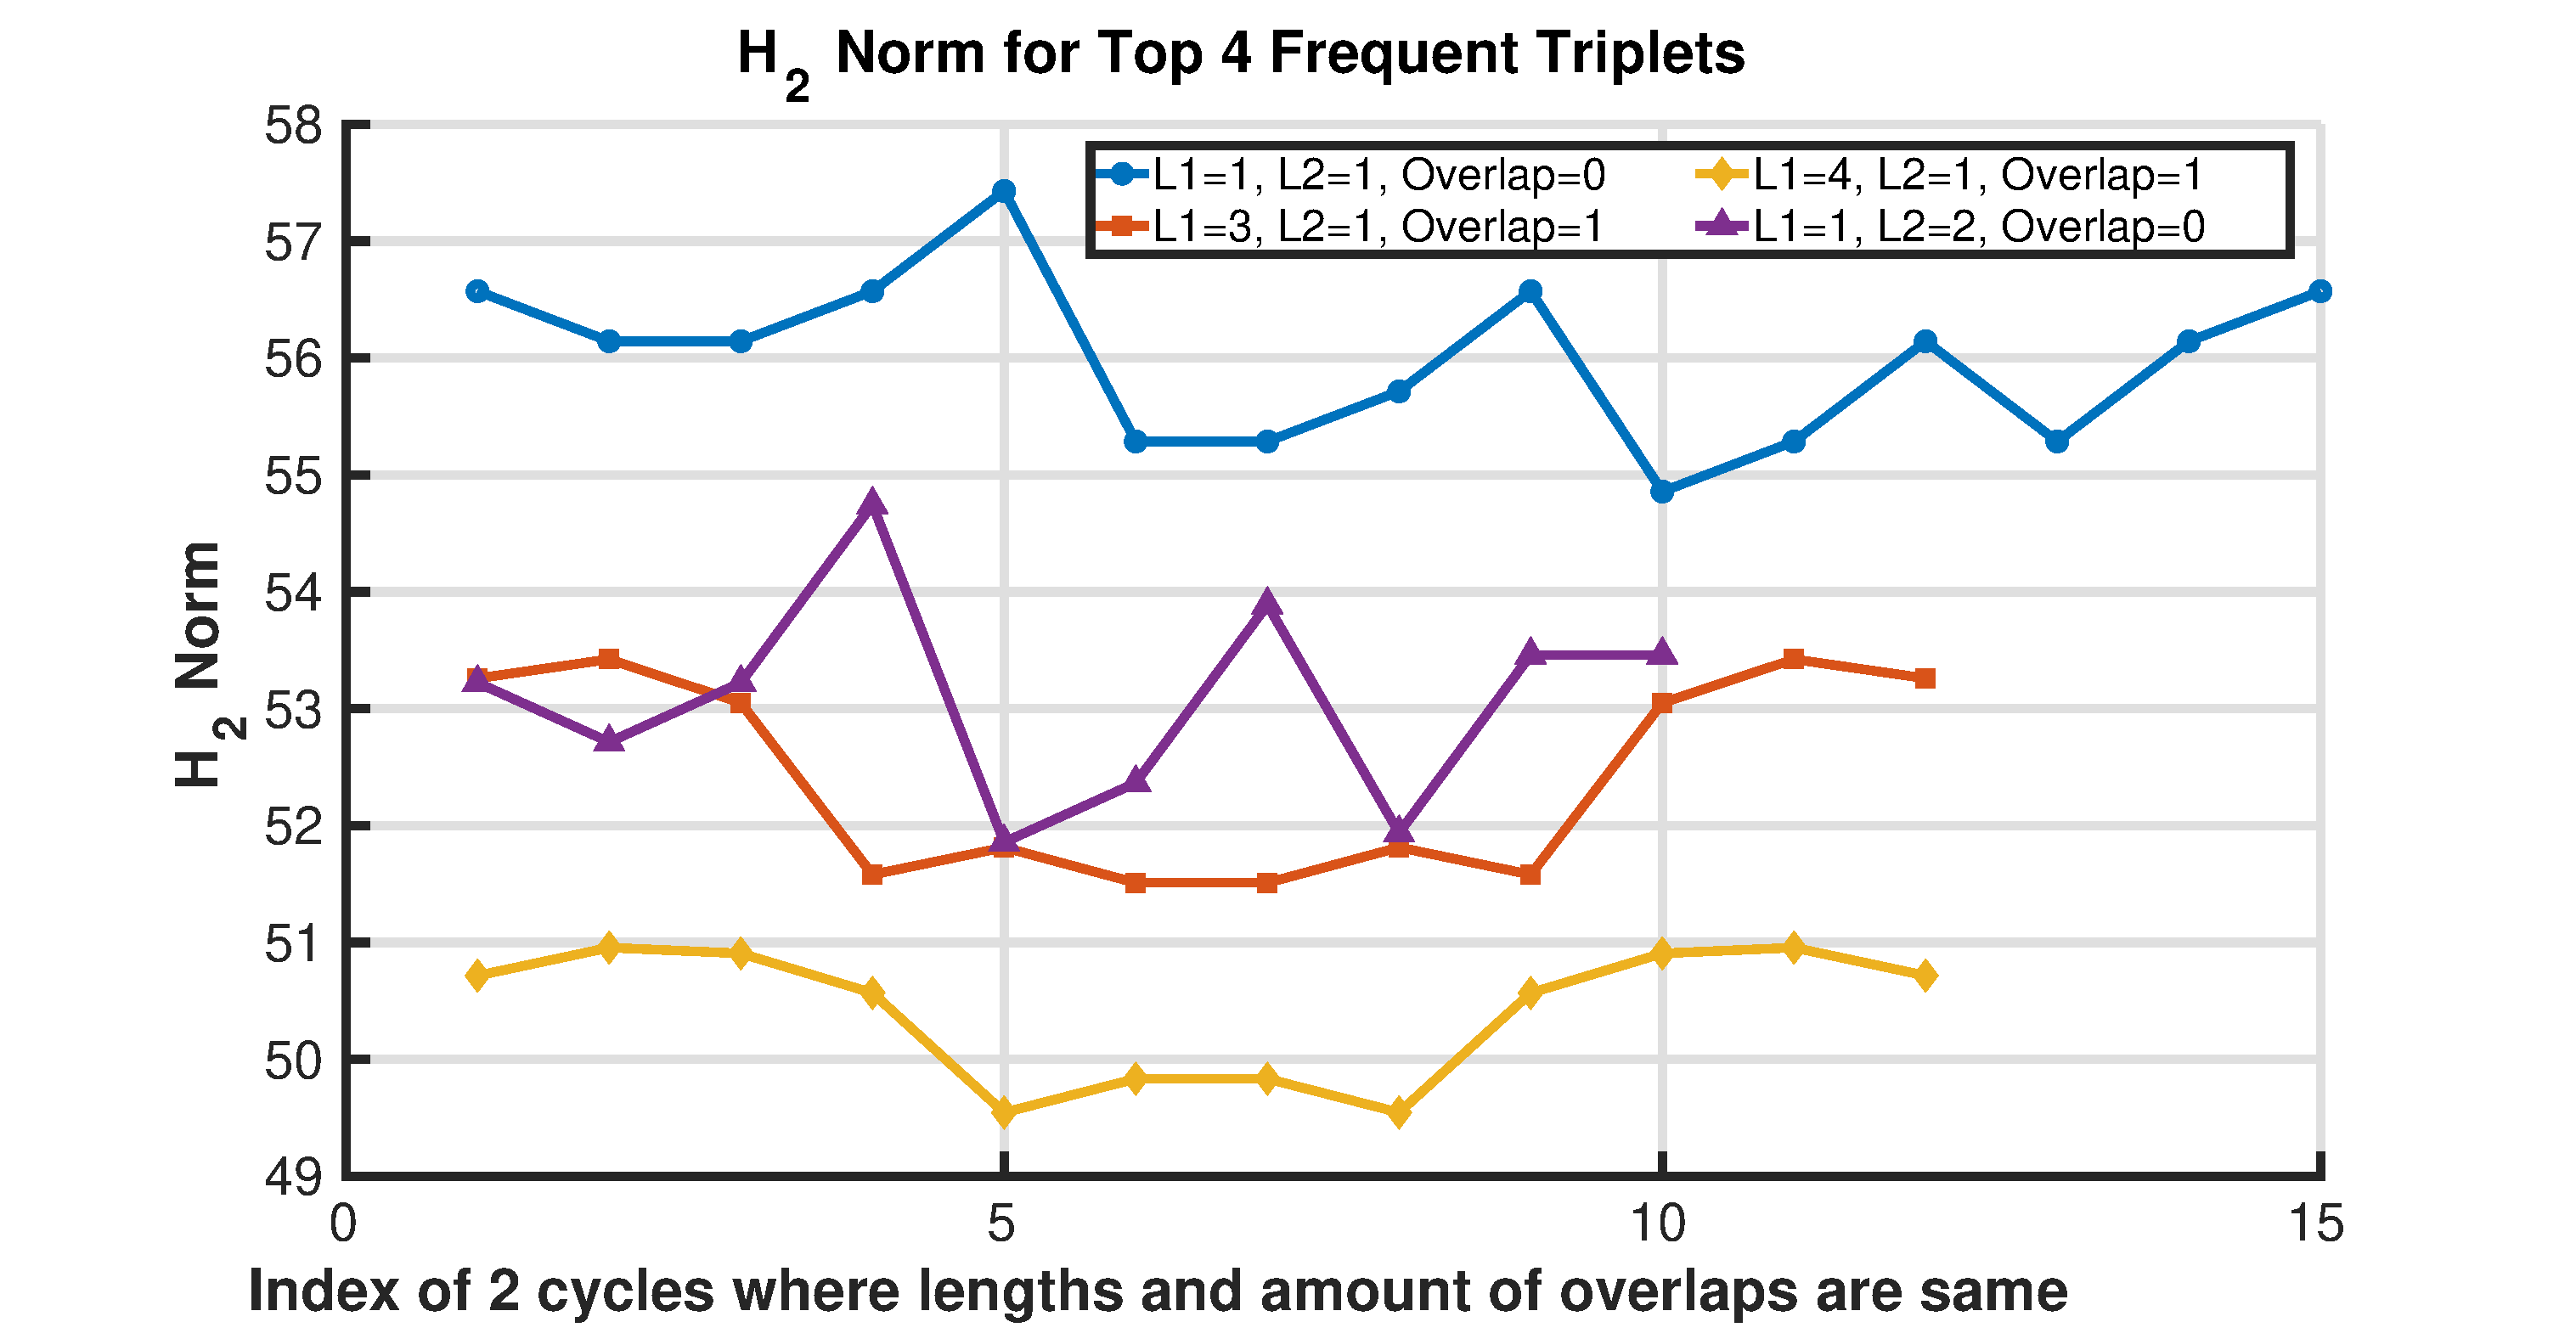
\includegraphics[width=0.8\textwidth, keepaspectratio]{4_Images/PositionalVariation.eps}
	\caption{Spatial position sensitivity: Minimization of $\|\Sigma\|_2^2$ }
	\label{fig:Position_dependence}
\end{figure}


\section{Summary}\label{sec:ch_RA_conclusion}
In this chapter, an analytical $\mathcal{H}_2$ performance framework was formulated for double-integrator multi-agent networks operating over cyclic graphs. The primary analytical conclusions are summarized as follows:

\begin{itemize}
    \item \textbf{Double-Integrator Energy Overhead:} Double-integrator networks inherently store disturbance energy within their physical velocity states ($\text{trace}(X_3) > 0$), resulting in a strictly larger $\mathcal{H}_2$ norm than single-integrator networks operating over identical topologies.
    \item \textbf{Spatial Locality Dependency:} Unlike first-order networks (where all spanning trees and cycle locations yield identical $\mathcal{H}_2$ norms), double-integrator performance depends strictly on the choice of spanning tree and the spatial placement of cycles. Specifically, placing a cycle near the spatial center of a path graph ($n_c = \frac{n+1}{2}$) maximizes systemic noise attenuation.
    \item \textbf{Optimal Cycle Overlap Bounds:} For dual-cycle topologies, moderate edge overlap ($s \le \frac{n+1}{6}$) strictly outperforms completely disjoint cycles, providing optimal noise suppression under environmental process and measurement disturbances.
\end{itemize}
\vspace{0.5em}
\noindent %\textbf{Transition to Chapter 5:}\\
While Chapters \ref{ch:TwoReverseEdges}, \ref{ch:Guaranteed_Consensus}, and \ref{ch:Robustness_Analysis} established exact dynamic consensus boundaries, localized gain tuning remedies, and $\mathcal{H}_2$ noise attenuation metrics across multi-agent communication graphs, real-world autonomous agents (such as mobile robots and unmanned aerial vehicles) must also navigate physical spatial environments under nonholonomic kinematic constraints.

To bridge graph-theoretic cooperative control with real-time physical motion execution, Chapter \ref{ch:Dubins_Path} and \ref{ch:Spiral_Path} shift their focus to local trajectory generation. Specifically, Chapter \ref{ch:Dubins_Path} formulates constrained path planning frameworks utilizing Dubins-like trajectories subject to terminal approach angle and impact time constraints.

\chapter[Dubins-Type Trajectory Synthesis Under Terminal Constraints]{Dubins-Type Trajectory Synthesis Under Approach Angle and Arrival Time Constraints\footnote{Some of the theoretical algorithms and formulations in this chapter are derived in part from the author's published work in the \emph{Proceedings of the Mediterranean Conference on Control and Automation (MED) 2024}. This chapter expands upon those preliminary results by providing complete derivations, closed-loop implementation, and comparative lateral acceleration analyses.}}\label{ch:Dubins_Path}
\section{Introduction and Physical Motivation}\label{sec:ch_DP_intro}
In preceding chapters, our investigation focused on distributed multi-agent consensus, establishing exact spectral stability boundaries (Chapter \ref{ch:TwoReverseEdges}), local edge/node scaling remedies (Chapter \ref{ch:Guaranteed_Consensus}), and $\mathcal{H}_2$ performance optimization (Chapter \ref{ch:Robustness_Analysis}). However, executing cooperative team maneuvers in physical environments requires individual autonomous vehicles— such as mobile robots, unmanned aerial vehicles (UAVs), or aerospace interceptors— to execute precise spatial trajectories under nonholonomic kinematic constraints, finite acceleration limits, and specific boundary conditions.

Several guidance and motion planning strategies have emerged in recent years aiming not only to achieve spatial target interception, but also to satisfy simultaneous terminal constraints, such as final impact (approach) angle, terminal time, or both. These dual constraints are critical across various technological applications. For instance, in coordinated robotic manipulation and multi-UAV salvo attacks, controlling the terminal time of arrival guarantees synchronous team convergence. Concurrently, controlling the final approach angle optimizes warhead penetration, aligns sensor fields of view, or avoids defensive countermeasure zones.

Prior literature has extensively explored single-constraint guidance strategies. Target interception under terminal impact angle constraints has been investigated using optimal guidance with time-to-go estimates \cite{zhao2015terminal}, seeker field-of-view constrained guidance \cite{park2013optimal}, biased proportional navigation (BPNG) \cite{kim1998BPNG}, and finite-time sliding mode control \cite{kumar2012sliding}. Similarly, standalone terminal time control has been tackled using feedback linearization \cite{Tekin2016_IT}, Lyapunov-based error dynamics convergence \cite{kim2014lyapunov}, and adaptive sliding mode control \cite{Chen2018_IT}. 

However, achieving \textbf{simultaneous control of both impact angle and terminal time} remains a major practical challenge. Existing dual-constraint methods, such as backstepping protocols \cite{Jung2006}, augmented proportional navigation variants \cite{Zhang2013, Zhang2015}, and multi-mode hybrid switching laws \cite{Harrison2012}, suffer from critical operational drawbacks:
\begin{enumerate}
    \item \textbf{Complex or Discontinuous Acceleration Demands:} They frequently require high-order, continuous time-varying, or infinitely switching (chattering) acceleration profiles that exceed physical actuator bounds ($a_M > a^{\max}$).
    \item \textbf{Inaccurate Time-to-Go Dependencies:} They rely heavily on linear small-angle approximations and time-to-go ($t_{\text{go}}$) estimates that degrade significantly under large heading error angles ($\theta_M \to \pi/2$).
\end{enumerate}

To overcome these limitations, this chapter proposes a computationally efficient, geometrically exact trajectory planning framework utilizing \textbf{Dubins-like path geometry} subject to maximum lateral acceleration bounds ($a^{\max}$). Though the engagement considered in this chapter is a one-on-one scenario (single interceptor against a single target), extensions of this framework to cooperative interception remains a future goal. 

\subsection*{Summary of Key Contributions}
The primary analytical and algorithmic contributions of this chapter are summarized as follows:
\begin{enumerate}
    \item \textbf{Piecewise-Constant Acceleration Profile:} We formulate an open-loop and equivalent closed-loop guidance scheme that requires only three discrete lateral acceleration levels ($+a^{\max}, 0, -a^{\max} \frac{r_m}{r_d}$), eliminating high-order polynomial computation and actuator saturation.
    \item \textbf{Flexible Terminal Time Tuning via Design Radius $r_d$:} Unlike classical Dubins paths \cite{hota2009modified} that utilize two circles of identical minimum turn radius ($r_m = V_M^2 / a^{\max}$) to minimize mission time, we introduce a variable secondary turn radius $r_d \ge r_m$. By adjusting $r_d$, the overall path length (and hence terminal arrival time $t_{\text{imp}}$) may be continuously tuned for any desired approach angle $\theta_t$.
    \item \textbf{Elimination of Feasible Upper Bounds on terminal time via Mirrored Geometry:} We show that when the launch and the approach angles share the same sign, Transverse Common Tangent (TCT) paths have a critical geometric upper bound $r_{\text{crit}}^{\text{TCT}}$. We resolve this limitation by introducing a mirrored TCT circle configuration, rendering the achievable terminal time unbounded above.
    \item \textbf{Singularity-Free Closed-Loop Implementation:} We derive a closed-loop state-feedback implementation governed by distance-to-go switching logic, proving that the guidance law remains non-singular even for large initial heading errors ($\theta_M \approx \pi/2$).
\end{enumerate}

\section{Engagement Kinematics and Problem Formulation}\label{sec:ch_DP_probform}

In this section, we present the mathematical modeling of the two-dimensional interceptor-target engagement scenario and formally state the dual-constraint trajectory planning problem. 

\subsection{Engagement Kinematics and Coordinate System}\label{subsec:ch_DP_kinematics}
Consider the planar engagement geometry depicted in Figure \ref{fig:ch_DP_eng_geometry}, where an autonomous point-mass interceptor pursues a stationary target. The target is located at Cartesian coordinates $(x_T, y_T)$ within an inertial reference frame $\mathcal{F}_I = \{\mathcal{O}; X, Y\}$. Without loss of generality, the origin $\mathcal{O}(0,0)$ is fixed at the interceptor's initial launch position at time $t = 0$.
\begin{figure}[ht!]
	\centering
	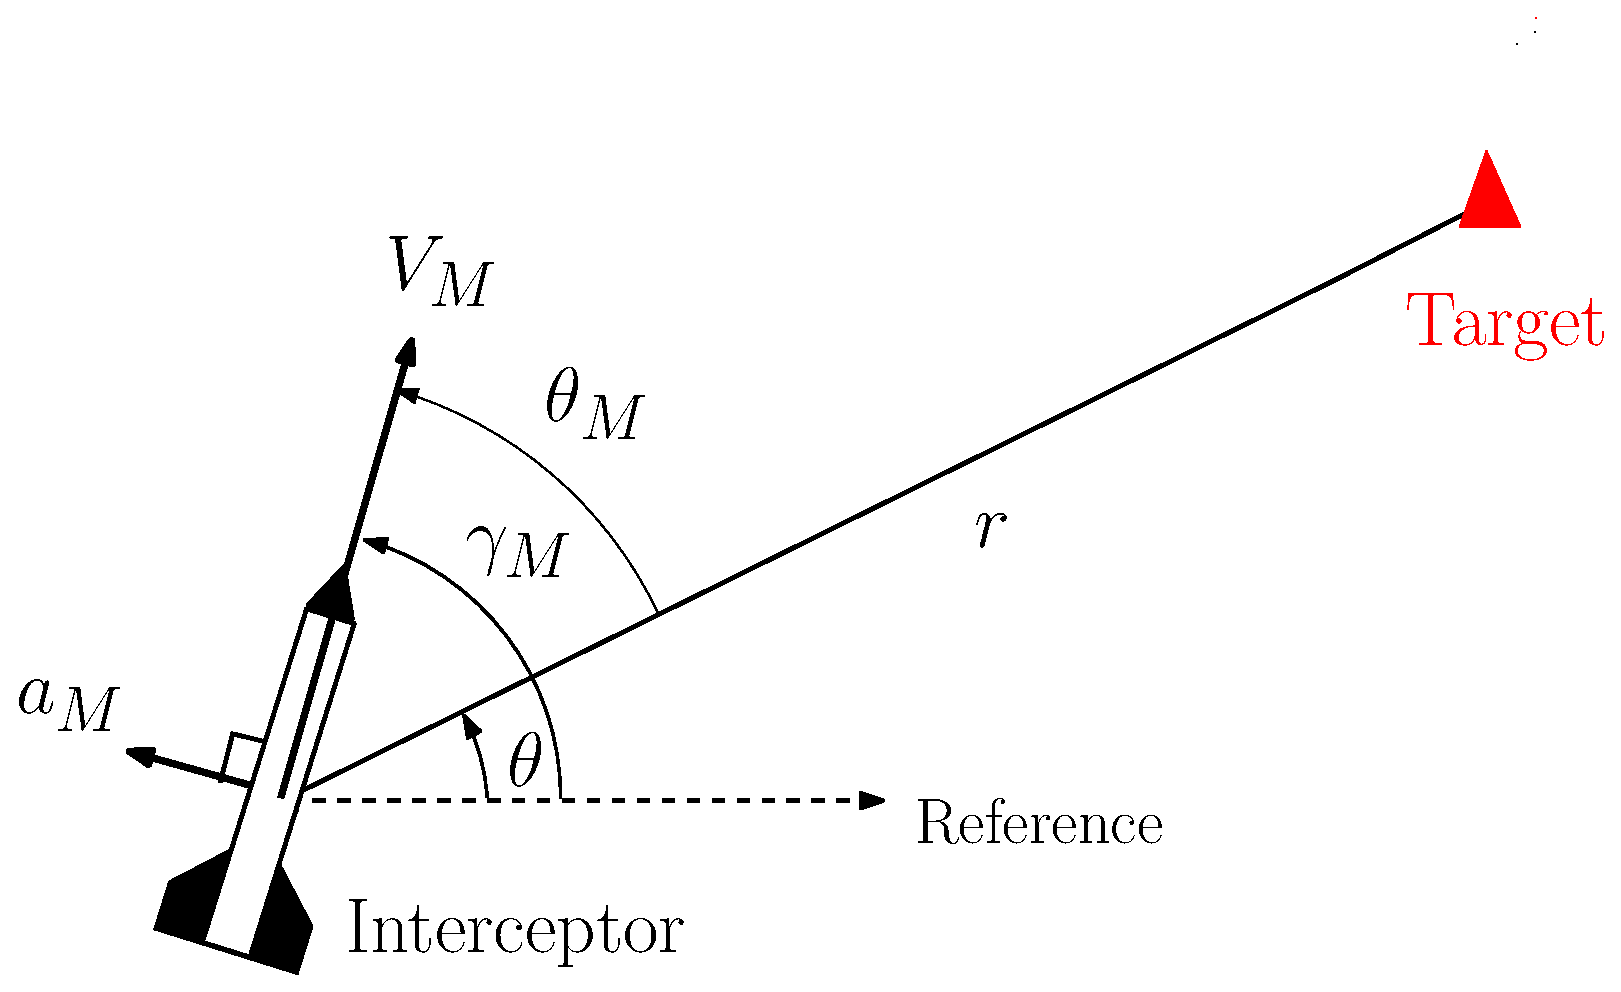
\includegraphics[width=0.8\textwidth, keepaspectratio]{5_Images/dubins_eng.eps}
	\caption{Planar engagement geometry between an autonomous interceptor and a stationary target.}
	\label{fig:ch_DP_eng_geometry}
\end{figure}

Let $(x_M(t), y_M(t))$ denote the position of the interceptor at time $t \ge 0$. The interceptor moves with a constant speed $V_M > 0$, and its instantaneous velocity direction is defined by the flight path angle $\gamma_M(t)$, measured counterclockwise with respect to the global $X$-axis. The control input governing the vehicle's trajectory is the commanded lateral acceleration $a_M(t)$, acting perpendicular to the velocity vector. Consequently, the Cartesian state dynamics of the interceptor are modeled as:
\begin{align}
	\dot{x}_M(t) &= V_M \cos \gamma_M(t), \label{eq:ch_DP_cart_x} \\
	\dot{y}_M(t) &= V_M \sin \gamma_M(t), \label{eq:ch_DP_cart_y} \\
	\dot{\gamma}_M(t) &= \frac{a_M(t)}{V_M}. \label{eq:ch_DP_gamma_dot}
\end{align}

To facilitate guidance law design, the relative kinematics are transformed into polar coordinates $(r, \theta)$, where $r(t)$ denotes the relative range between the interceptor and the target, and $\theta(t)$ denotes the line-of-sight (LOS) angle with respect to the $X$-axis:
\begin{equation}\label{eq:ch_DP_polar_defs}
	r(t) = \sqrt{\big(x_T - x_M(t)\big)^2 + \big(y_T - y_M(t)\big)^2}, \quad \theta(t) = \operatorname{arctan}\Big(y_T - y_M(t), \, x_T - x_M(t)\Big).
\end{equation}

By aligning the initial LOS angle along the horizontal axis ($\theta(0) = 0$), the stationary target's coordinates simplify to $(r(0), 0) = (r_0, 0)$, where $r_0 > 0$ represents the initial range-to-go. The nonholonomic engagement dynamics in polar coordinates are governed by:
\begin{align}
	\dot{r}(t) &= -V_M \cos \theta_M(t), \label{eq:ch_DP_rdot} \\
	r(t) \dot{\theta}(t) &= -V_M \sin \theta_M(t), \label{eq:ch_DP_thetadot}
\end{align}
where $\theta_M(t) \coloneqq \gamma_M(t) - \theta(t)$ represents the lead angle (or look angle) of the interceptor relative to the LOS vector. Equations \eqref{eq:ch_DP_cart_x}--\eqref{eq:ch_DP_thetadot} constitute the complete set of non holonomic kino-dynamic constraints governing planar pursuit.
\subsection{Actuator Limits and Minimum Turn Radius}\label{subsec:ch_DP_actuator_limits}
In practical aerospace and robotic platforms, the commanded lateral acceleration $a_M(t)$ is strictly bounded by structural limits, maximum angle-of-attack thresholds, or motor saturation. We enforce the hard inequality constraint:
\begin{equation}\label{eq:ch_DP_accel_bound}
	|a_M(t)| \le a^{\max}, \quad \forall t \in [0, t_{\text{imp}}],
\end{equation}
where $a^{\max} > 0$ is the maximum allowable lateral acceleration. Substituting constraint \eqref{eq:ch_DP_accel_bound} into kinematic relation \eqref{eq:ch_DP_gamma_dot} establishes a maximum turn rate $\dot{\gamma}_M^{\max} = a^{\max} / V_M$. This physical constraint dictates a fundamental lower bound on the instantaneous radius of curvature of the flight trajectory, termed the minimum turn radius $r_m$:
\begin{equation}\label{eq:ch_DP_min_radius}
	r_m \coloneqq \frac{V_M^2}{a^{\max}}.
\end{equation}
Any admissible geometric path synthesized for the interceptor must possess a local radius of curvature $R(t) \ge r_m$ everywhere along its spatial length.
\subsection{Terminal Constraints and Formal Problem Statement}\label{subsec:ch_DP_problem_statement}
Precision target engagements require enforcing boundary conditions not only on target interception ($r(t_{\text{imp}}) = 0$), but also on the direction of arrival (impact angle) and the total mission time (impact time).
\begin{definition}[Terminal/Impact Time]\label{def:ch_DP_impact_time}
The terminal impact time $t_{\text{imp}} > 0$ is the total elapsed time from interceptor launch ($t = 0$) to target interception ($r(t_{\text{imp}}) = 0$). For a constant flight speed $V_M$, the impact time is directly proportional to the spatial arc length $P$ of the trajectory:
\begin{equation}\label{eq:ch_DP_impact_time_def}
	t_{\text{imp}} = \int_0^{t_{\text{imp}}} \mathrm{d}t = \frac{1}{V_M} \int_0^P \mathrm{d}s = \frac{P}{V_M}.
\end{equation}
\end{definition} 

\begin{definition}[Impact Angle]\label{def:ch_DP_impact_angle}
\leavevmode\par\noindent
The terminal impact angle $\theta_t \in (-\pi, \pi]$ is defined as the orientation of the interceptor's velocity vector relative to the global reference $X$-axis at the precise instant of target interception ($t = t_{\text{imp}}$):
\begin{equation}\label{eq:ch_DP_approach_def}
	\theta_t \coloneqq \lim_{t \to t_{\text{imp}}} \gamma_M(t).
\end{equation}
\end{definition}



With these definitions established, we formally state the dual-constraint trajectory planning problem investigated in this chapter:

\begin{problem}\label{prob:ch_DP_main_problem}
Given an interceptor's initial state vector $\mathbf{x}(0) = [x_M(0), y_M(0), \gamma_M(0)]^T = [0, 0, \gamma_M(0)]^T$, constant speed $V_M$, target initial location $(r_0, 0)$, and maximum lateral acceleration capability $a^{\max}$, synthesize a computationally efficient, singularity-free guidance law $a_M(t)$ such that the following conditions are met:
\begin{enumerate}
    \item \textbf{Target Interception:} The interceptor reaches the target position at time $t = t_{\text{imp}}$, satisfying $r(t_{\text{imp}}) = 0$.
    \item \textbf{Impact Angle Satisfaction:} The velocity vector aligns with the desired approach angle at interception: $\gamma_M(t_{\text{imp}}) = \theta_t$.
    \item \textbf{Impact Time Satisfaction:} Interception occurs exactly at a designated feasible arrival time $t_{\text{imp}} = t^{\star}$.
    \item \textbf{Actuator Feasibility:} The lateral acceleration input satisfies the strict bound $|a_M(t)| \le a^{\max}$ for all $t \in [0, t^{\star}]$.
\end{enumerate}
\end{problem}

\section{Dubins-Like Guidance Path Synthesis}\label{sec:ch_DP_main_design}

In this section, we present the geometric construction of the proposed trajectory planning framework. We first review classic Dubins path theory and discuss its limitations regarding time-of-arrival control, before introducing our variable-radius Dubins-like trajectory architecture.
\subsection{Foundational Principles: Classic Dubins Path Theory and Limitations}\label{subsec:ch_DP_dubins_theory}

The classic path-planning problem formulated by L.E. Dubins (1957) addresses finding the shortest bounded-curvature path between an initial configuration $(x_0, y_0, \theta_0)$ and a final configuration $(x_f, y_f, \theta_f)$ in a two-dimensional Euclidean plane. 

Dubins proved that the optimal trajectory minimizing total path length $P$ belongs to a finite family of paths composed of at most three sequential primitive segments: circular arcs of minimum turn radius $r_m$ (denoted by $L$ for left turn and $R$ for right turn) and straight-line segments (denoted by $S$ for straight). The optimal path family is categorized into two distinct classes:
\begin{enumerate}
    \item \textbf{CSC Class:} Composed of two circular turns connected by a straight line tangent ($\text{LSL}, \text{RSR}, \text{LSR}, \text{RSL}$).
    \item \textbf{CCC Class:} Composed of three consecutive circular turns with alternating directions ($\text{LRL}, \text{RLR}$).
\end{enumerate}

While classic Dubins paths provide time-optimal (shortest-length) trajectories for reaching a target at a specified approach angle, they possess zero flexibility regarding time-of-arrival control. Because all circular arcs in a classic Dubins path are fixed at the minimum radius $r_m$, the total path length $P_{\text{min}}$ is uniquely determined by the initial and final boundary conditions. Consequently, the resulting impact time $t_{\text{imp}}^{\text{min}} = P_{\text{min}} / V_M$ is fixed. If an operational engagement demands a delayed arrival time ($t^{\star} > t_{\text{imp}}^{\text{min}}$) to coordinate salvo strikes or bypass dynamic defenses, classic Dubins paths cannot accommodate the requirement.
\subsection{Proposed Generalized Dubins-Like Path Architecture}\label{subsec:ch_DP_proposed_dubins_concept}

To overcome the temporal rigidity of classic Dubins paths while maintaining bounded acceleration demands ($|a_M(t)| \le a^{\max}$), we generalize the CSC path geometry. Instead of setting both turning radii equal to $r_m$, we assign the radius of the secondary turn circle, centered at the target location as a design parameter.

Specifically, the proposed Dubins-like trajectory consists of three sequential geometric segments:
\begin{enumerate}
	\item \textbf{Primary Circular Arc ($A_1$ on Circle $C_1$):} A turn executed at minimum turn radius $r_m \coloneqq V_M^2 / a^{\max}$ tangential to the interceptor's initial heading vector $\theta_m \coloneqq \theta_M(0)$. This guarantees the fastest initial heading reorientation.
	\item \textbf{Straight Line Tangent ($L_{\text{TCT}}$/$L_{\text{DCT}}$):} A linear segment ($a_M = 0$) directed along the Transverse Common Tangent (TCT) or Direct Common Tangent (DCT) connecting primary circle $C_1$ and secondary circle $C_2$.
	\item \textbf{Secondary Circular Arc ($A_2$ on Circle $C_2$):} A turn executed at a \emph{variable design radius} $r_d \ge r_m$ centered at location $D$, tangential to the target position $(r_0, 0)$ at the desired approach angle $\theta_t$.
\end{enumerate}

By choosing the secondary circle radius $r_d$ as a continuous control design variable ($r_d \in [r_m, r_{\text{crit}}]$), the spatial path length $P(r_d)$ and consequently the terminal arrival time $t_{\text{imp}}(r_d) = P(r_d) / V_M$ becomes a continuously tunable function. Furthermore, enforcing $r_d \ge r_m$ guarantees that the commanded lateral acceleration on circle $C_2$ satisfies:
\begin{equation}\label{eq:ch_DP_rd_accel_bound}
	|a_M|_{C_2} = \frac{V_M^2}{r_d} = a^{\max} \left(\frac{r_m}{r_d}\right) \le a^{\max},
\end{equation}
thereby strictly respecting physical actuator bounds throughout the entire maneuver.

\subsection{TCT Path Geometry with `Same-Sign' Angles}\label{sec:ch_DP_tct_same_sign}
We first analyze the geometric construction when the initial launch angle $\theta_m \in (0, \pi)$ and the terminal approach angle $\theta_t \in (0, \pi)$ share identical algebraic signs (positive counterclockwise orientation relative to the LOS reference), as illustrated in Figure \ref{fig:ch_DP_TCT_samesign}.

\begin{figure}[ht!]
	\centering
	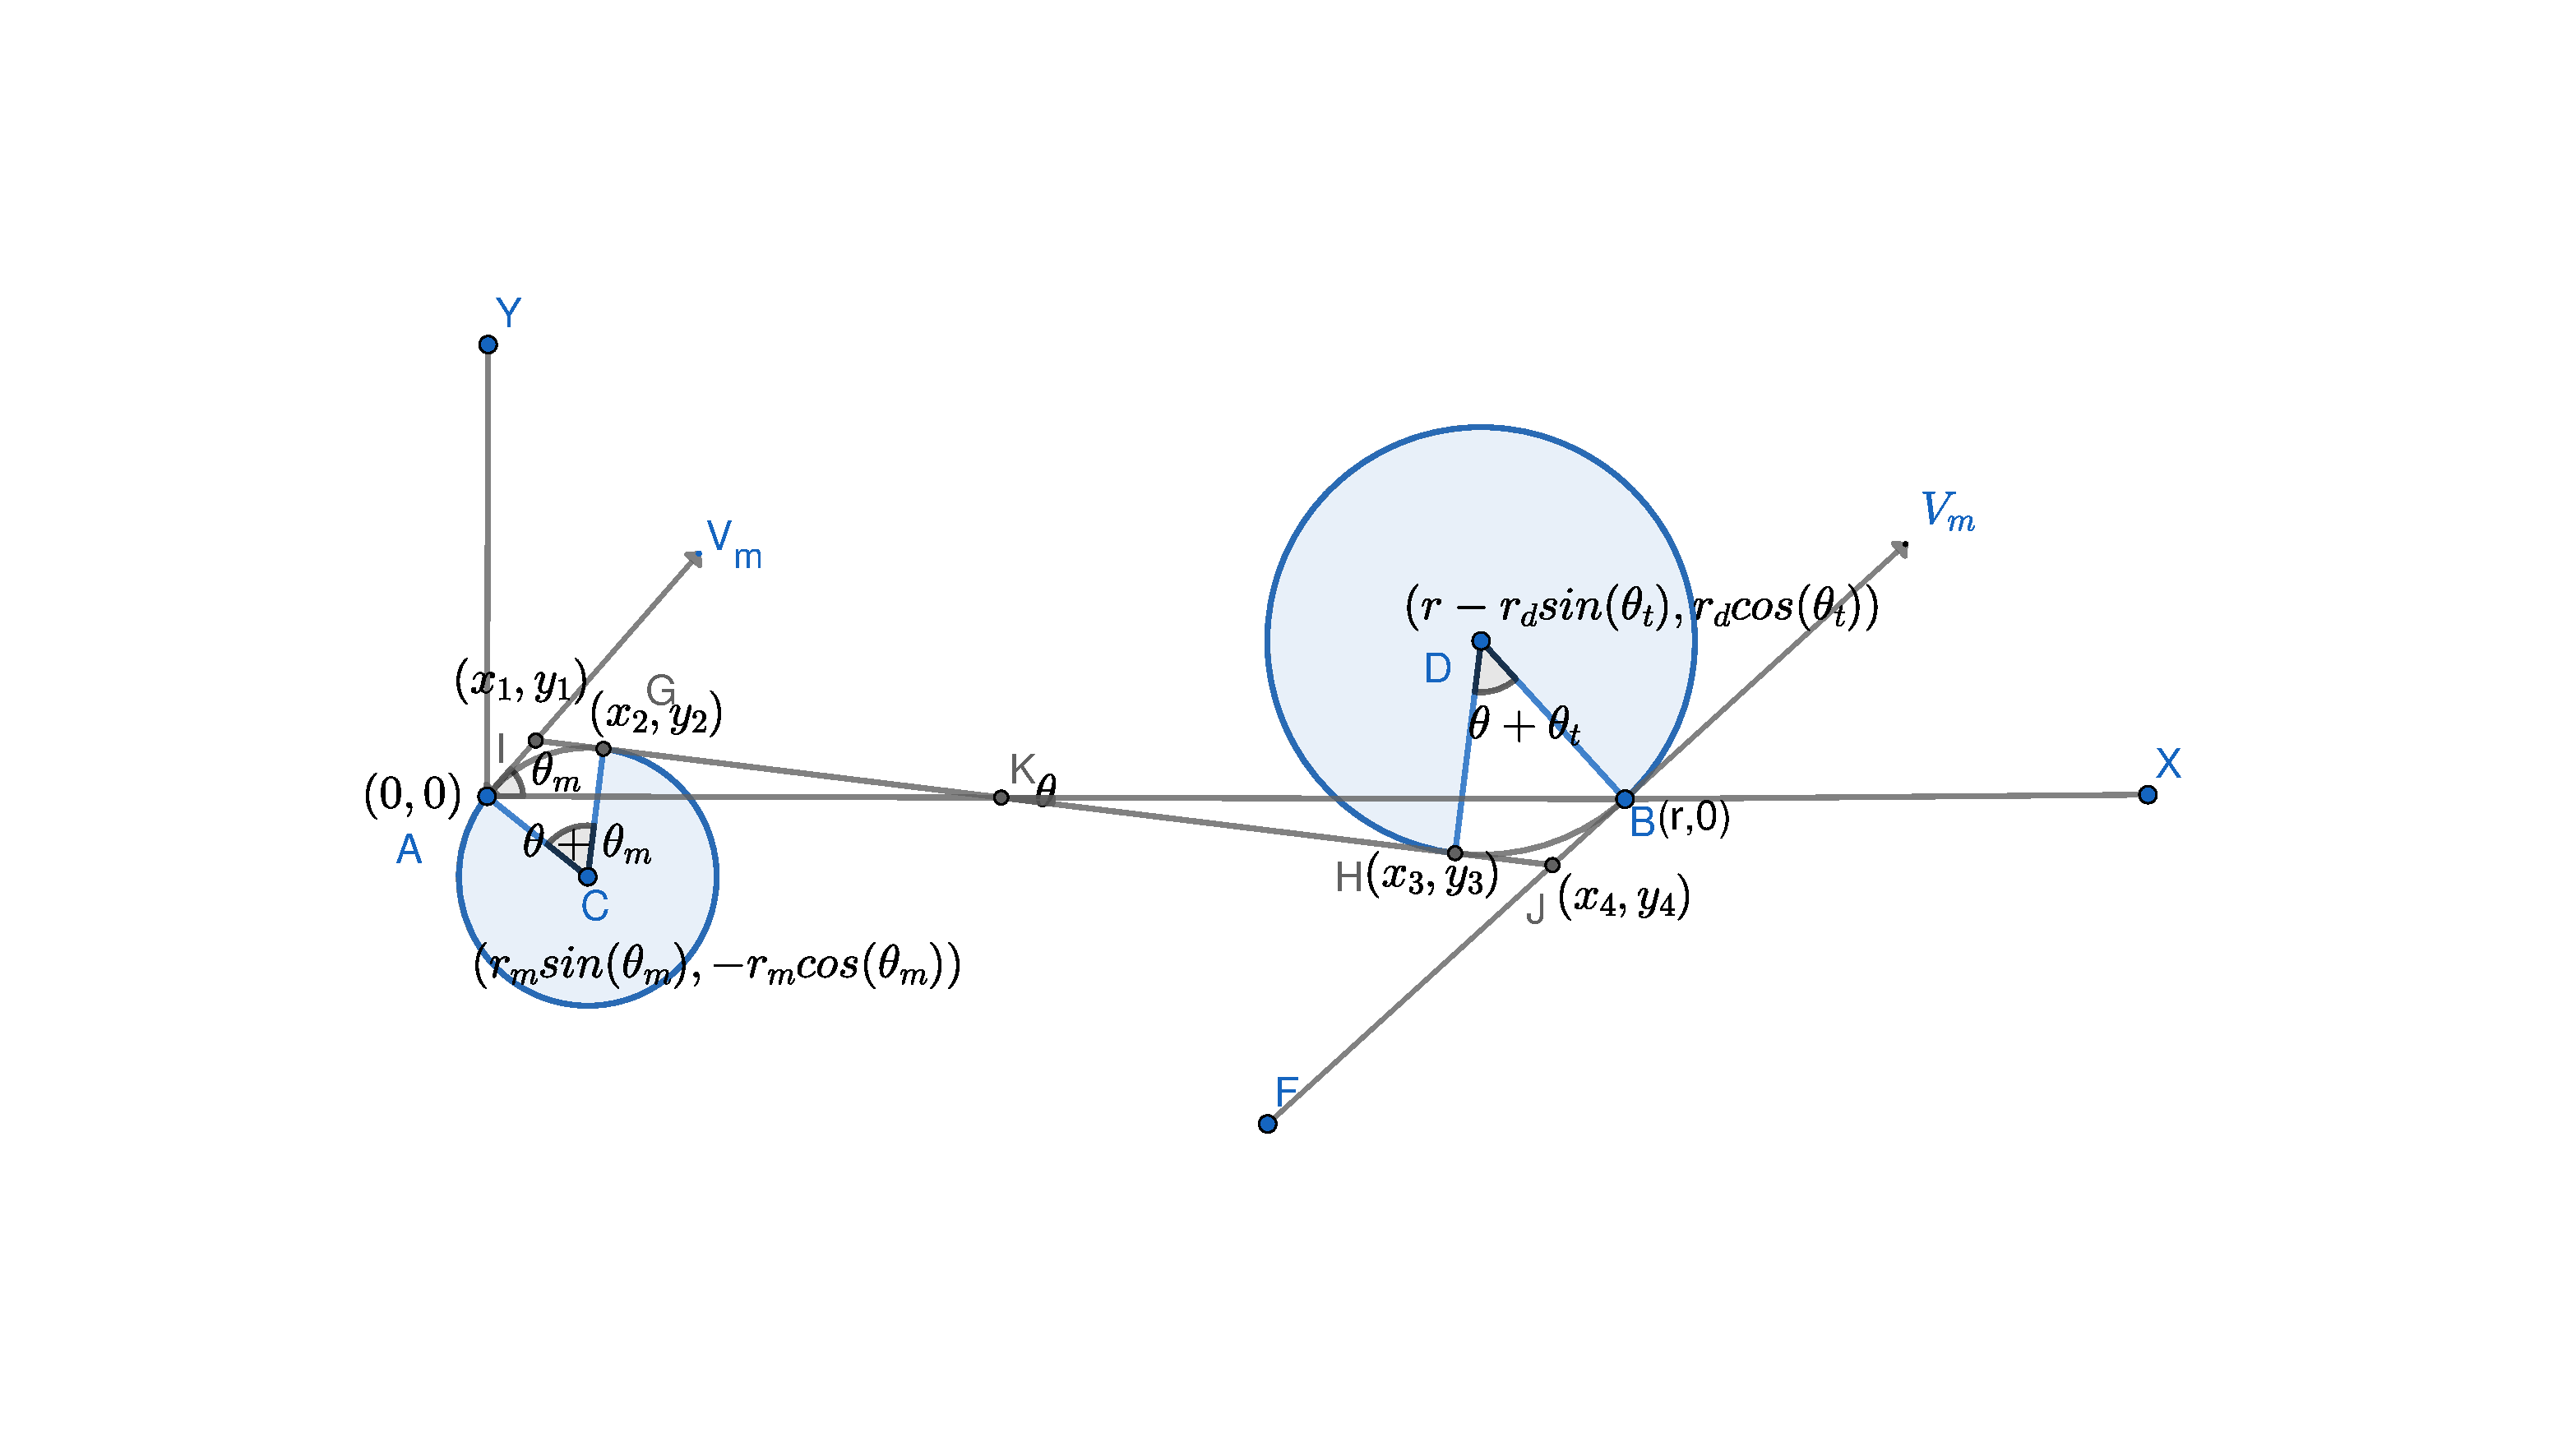
\includegraphics[width=\textwidth, keepaspectratio]{5_Images/TCT_New.pdf}
	\caption{Geometric construction of the TCT Dubins-like path when initial launch angle $\theta_m$ and approach angle $\theta_t$ share the same sign.}
	\label{fig:ch_DP_TCT_samesign}
\end{figure}

The center $C = (x_C, y_C)$ of primary circle $C_1$ and center $D = (x_D, y_D)$ of secondary circle $C_2$ are uniquely determined by vector tangency:
\begin{equation}\label{eq:ch_DP_centers_samesign}
	C = \big(r_m \sin \theta_m, \, -r_m \cos \theta_m\big), \quad D = \big(r - r_d \sin \theta_t, \, r_d \cos \theta_t\big),
\end{equation}
where $r = r_0$ is the initial target range.

The Euclidean distance $d(r_d) \coloneqq \|D - C\|_2$ between circle centers $C$ and $D$ is evaluated using the law of cosines:
\begin{align}\label{eq:ch_DP_center_distance}
	d^2(r_d) &= (r - r_d \sin \theta_t - r_m \sin \theta_m)^2 + (r_d \cos \theta_t + r_m \cos \theta_m)^2 \nonumber \\
	&= r^2 + r_d^2 + r_m^2 + 2 r_d r_m \cos(\theta_m - \theta_t) - 2 r (r_d \sin \theta_t + r_m \sin \theta_m).
\end{align}

For a valid Transverse Common Tangent segment $L_{\text{TCT}}$ to connect circles $C_1$ and $C_2$ externally without overlap, the center-to-center distance must satisfy the geometric condition $d(r_d) \ge r_m + r_d$. As $r_d$ increases, the two circles expand towards each other. The critical upper bound $r_{\text{crit}}^{\text{TCT}}$ occurs at exact circle contact where $d(r_{\text{crit}}^{\text{TCT}}) = r_m + r_{\text{crit}}^{\text{TCT}}$, causing $L_{\text{TCT}} \to 0$:
\begin{equation}\label{eq:ch_DP_rcrit_tct}
	r_{\text{crit}}^{\text{TCT}} = \frac{r^2 - 2 r r_m \sin \theta_m}{2 r_m \left(1 - \cos(\theta_m - \theta_t)\right) + 2 r \sin \theta_t}.
\end{equation}

To compute segment arc lengths, let line $AI$ represent the initial velocity tangent ($y = x \tan \theta_m$), line $BF$ represent the final velocity tangent ($y = (x - r) \tan \theta_t$), and line $IKJ$ denote the TCT segment ($y = -x \tan \theta + c$). Solving the linear intersection systems yields tangent lengths $L_{t1}$ on circle $C_1$ and $L_{t2}$ on circle $C_2$:
\begin{equation}\label{eq:ch_DP_tangent_lengths}
	L_{t1} = \frac{c}{\tan \theta_m + \tan \theta} \sec \theta_m, \quad L_{t2} = \frac{c + r \tan \theta}{\tan \theta_t + \tan \theta} \sec \theta_t,
\end{equation}
where $c = r_m (\cos \theta - \cos \theta_m + \sin \theta \tan \theta + \sin \theta_m \tan \theta)$.

The secondary circle radius $r_d$ relates to $L_{t2}$ via $r_d = L_{t2} \cot \left( \frac{\theta_t + \theta}{2} \right)$. The TCT length $L_{\text{TCT}}$ is obtained by projecting line segments onto the horizontal baseline:
\begin{equation}\label{eq:ch_DP_LTCT_expr}
	L_{\text{TCT}} = \frac{r - L_{t1}(\cos \theta_m + \cos \theta) - L_{t2}(\cos \theta_t + \cos \theta)}{\cos \theta}.
\end{equation}

The total path length $P(r_d)$ for $r_d \in [r_m, r_{\text{crit}}^{\text{TCT}})$ is the sum of the three segment lengths:
\begin{equation}\label{eq:ch_DP_total_path_length}
	P(r_d) = A_1 + L_{\text{TCT}} + A_2 = r_m (\theta_m + \theta) + L_{\text{TCT}} + r_d (\theta_t + \theta),
\end{equation}
and the resulting terminal impact time is $t_{\text{imp}}(r_d) = P(r_d) / V_M$.
\subsection{Mirrored TCT Geometry for Unbounded Arrival Time}\label{sec:ch_DP_tct_mirrored}

While the standard TCT construction in Section \ref{sec:ch_DP_tct_same_sign} allows arrival time tuning, the existence of critical radius $r_{\text{crit}}^{\text{TCT}}$ imposes a upper bound on achievable impact time ($t_{\text{imp}} \le P(r_{\text{crit}}^{\text{TCT}}) / V_M$). When an engagement requires an exceptionally large arrival time, or when the launch angle and approach angle have opposite algebraic signs, circle $C_2$ is mirrored across the target baseline to position $C_2'$, as shown in Figure \ref{fig:ch_DP_TCT_opposite_sign}.

\begin{figure}[ht!]
	\centering
	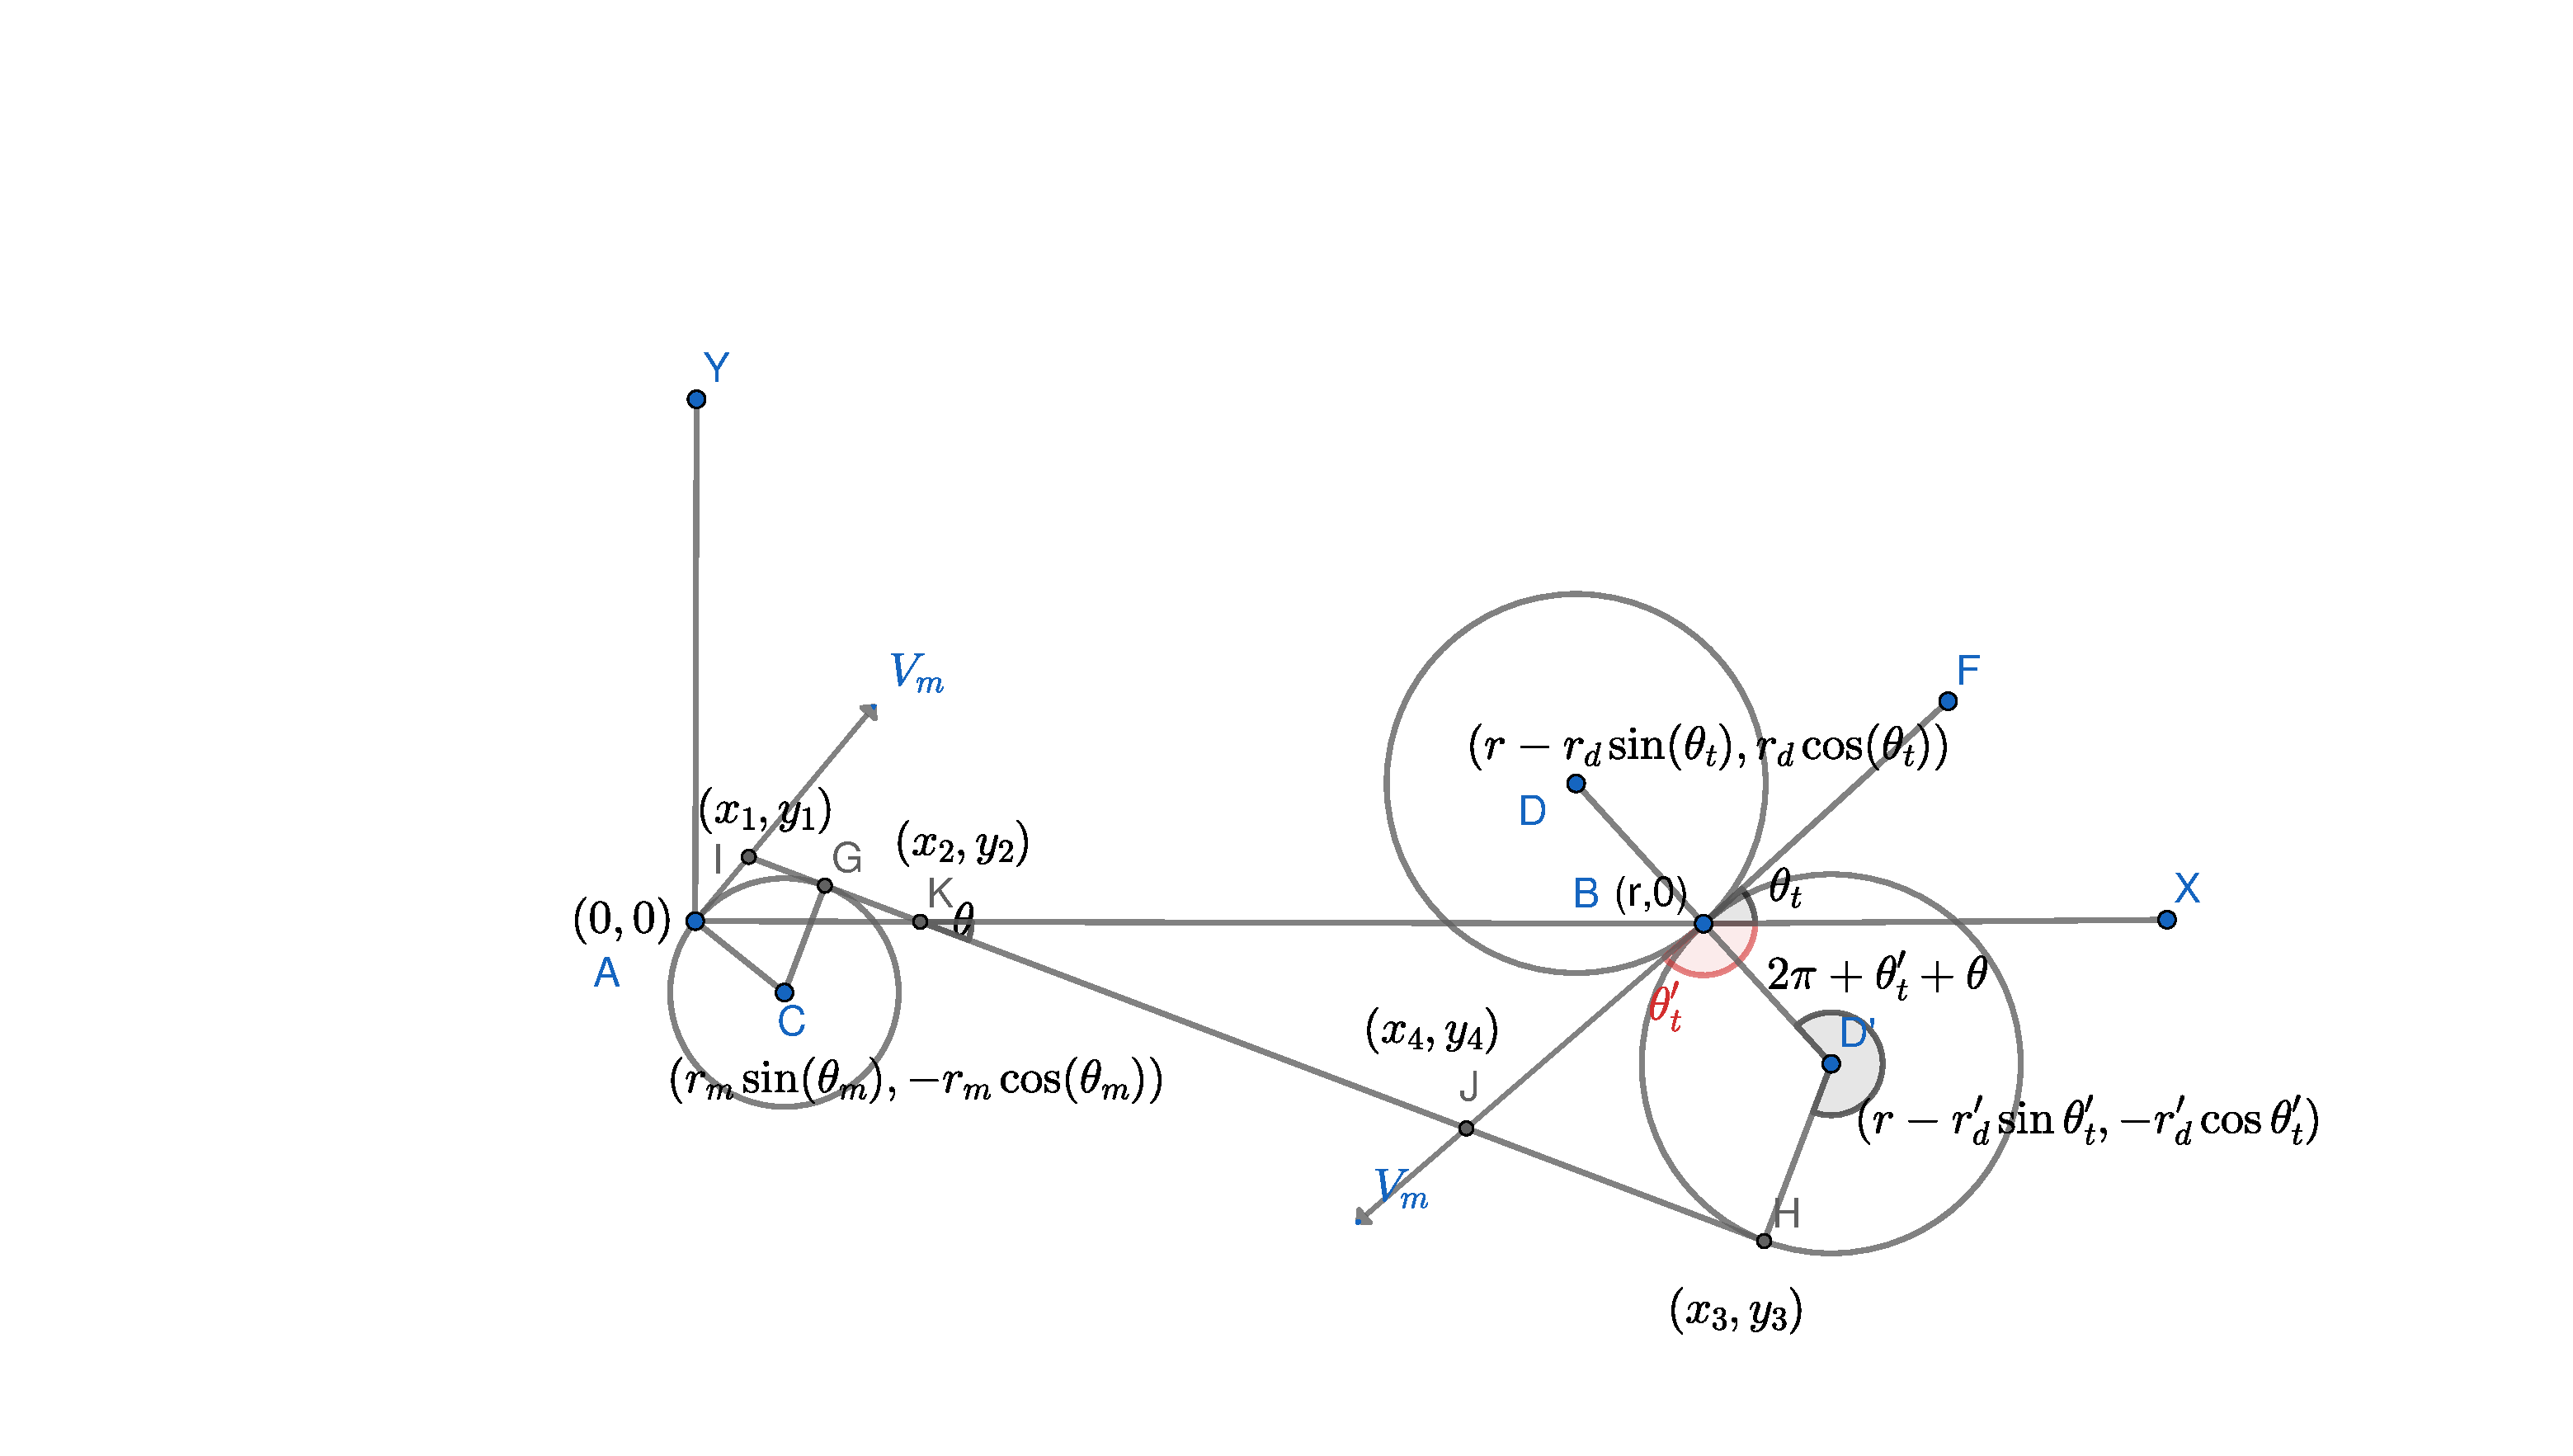
\includegraphics[width=\textwidth, keepaspectratio]{TCTExternal_New.pdf}
	\caption{Mirrored TCT Dubins-like path ($C_2'$), providing unbounded path length $P'(r_d')$ for large terminal time requirements.}
	\label{fig:ch_DP_TCT_opposite_sign}
\end{figure}

The mirrored circle center $D'$ is located at:
\begin{equation}\label{eq:ch_DP_mirrored_center}
	D' = \left( r - r_d' \sin \theta_t', \, -r_d' \cos \theta_t' \right).
\end{equation}

The center-to-center distance $d'(r_d')$ between $C_1$ and $D'$ may be given by:
\begin{equation}\label{eq:ch_DP_mirrored_distance}
	(d')^2 = r^2 + (r_d')^2 + r_m^2 - 2 r_d' r_m \cos(\theta_m + \theta_t') - 2 r (r_d' \sin \theta_t' + r_m \sin \theta_m).
\end{equation}

Because circle $C_2'$ lies on the opposite side of baseline $BF$, $d'(r_d')$ increases monotonically with $r_d'$ without intersecting $C_1$. Consequently, the upper bound constraint is eliminated, rendering the path length $P'(r_d')$ strictly unbounded above ($P' \to \infty$ as $r_d' \to \infty$).

The mirrored arc length traversed on circle $C_2'$ is $A_2' = r_d' (2\pi + \theta_t' + \theta)$, yielding the modified total path length:
\begin{equation}\label{eq:ch_DP_mirrored_path_length}
	P'(r_d') = r_m (\theta_m + \theta) + L_{\text{TCT}}' + r_d' (2\pi + \theta_t' + \theta).
\end{equation}
This mirrored geometry guarantees that any arbitrary, physically feasible impact time $t^{\star} \ge t_{\text{imp}}^{\text{min}}$ can be matched exactly by choosing a suitable radius $r_d'$.

\subsection{Extension to Direct Common Tangent (DCT) and Outer Circle Geometry}\label{subsec:ch_DP_dct_outer}

A geometric constraint of the TCT guidance scheme utilizing an \emph{inner} circle tangential to both launch and target points is the existence of an upper bound on achievable impact time ($t_{\text{imp}} \le P(r_{\text{crit}}^{\text{TCT}}) / V_M$). This bound stems from the critical radius threshold $r_{\text{crit}}^{\text{TCT}}$ at which the two inner circles intersect and the length of the transverse common tangent vanishes ($L_{\text{TCT}} \to 0$).

To overcome this upper bound without requiring vehicle re-orientation or mirrored baseline maneuvers, an alternative construction employs an \emph{outer} circle tangential to the desired velocity vector drawn at the target location, or utilizes a Direct Common Tangent (DCT) configuration. The geometric constructions for TCT and DCT paths with outer circles are depicted in Figure \ref{fig:ch_DP_outer_tct_dct}.

\begin{figure}[!ht]
	\centering
	\begin{subfigure}[b]{0.7\textwidth}
		\centering
		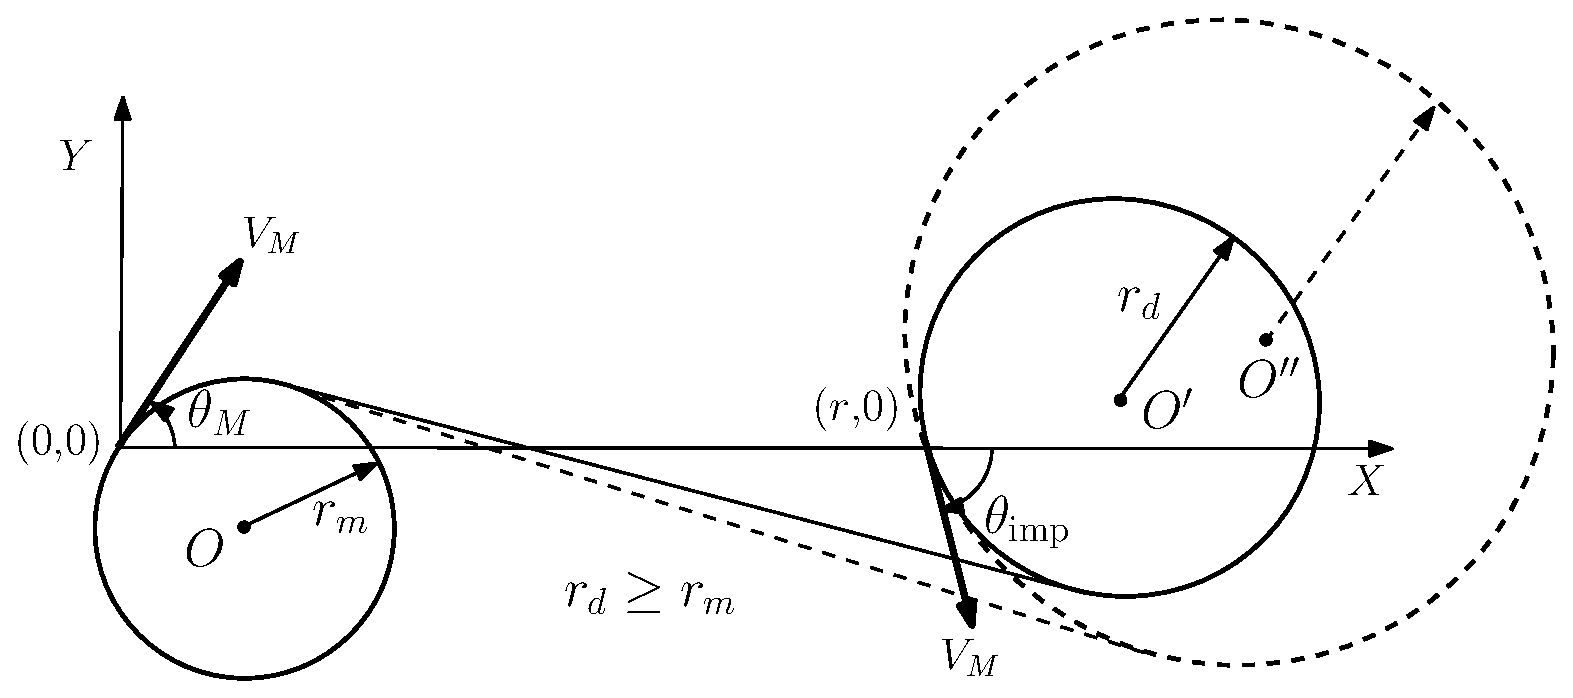
\includegraphics[width=\textwidth]{fig44.eps}
		\caption{Transverse common tangent (TCT) path.}
		\label{fig:ch_DP_figtct}
	\end{subfigure}
	\hfill
	\begin{subfigure}[b]{0.7\textwidth}
		\centering
		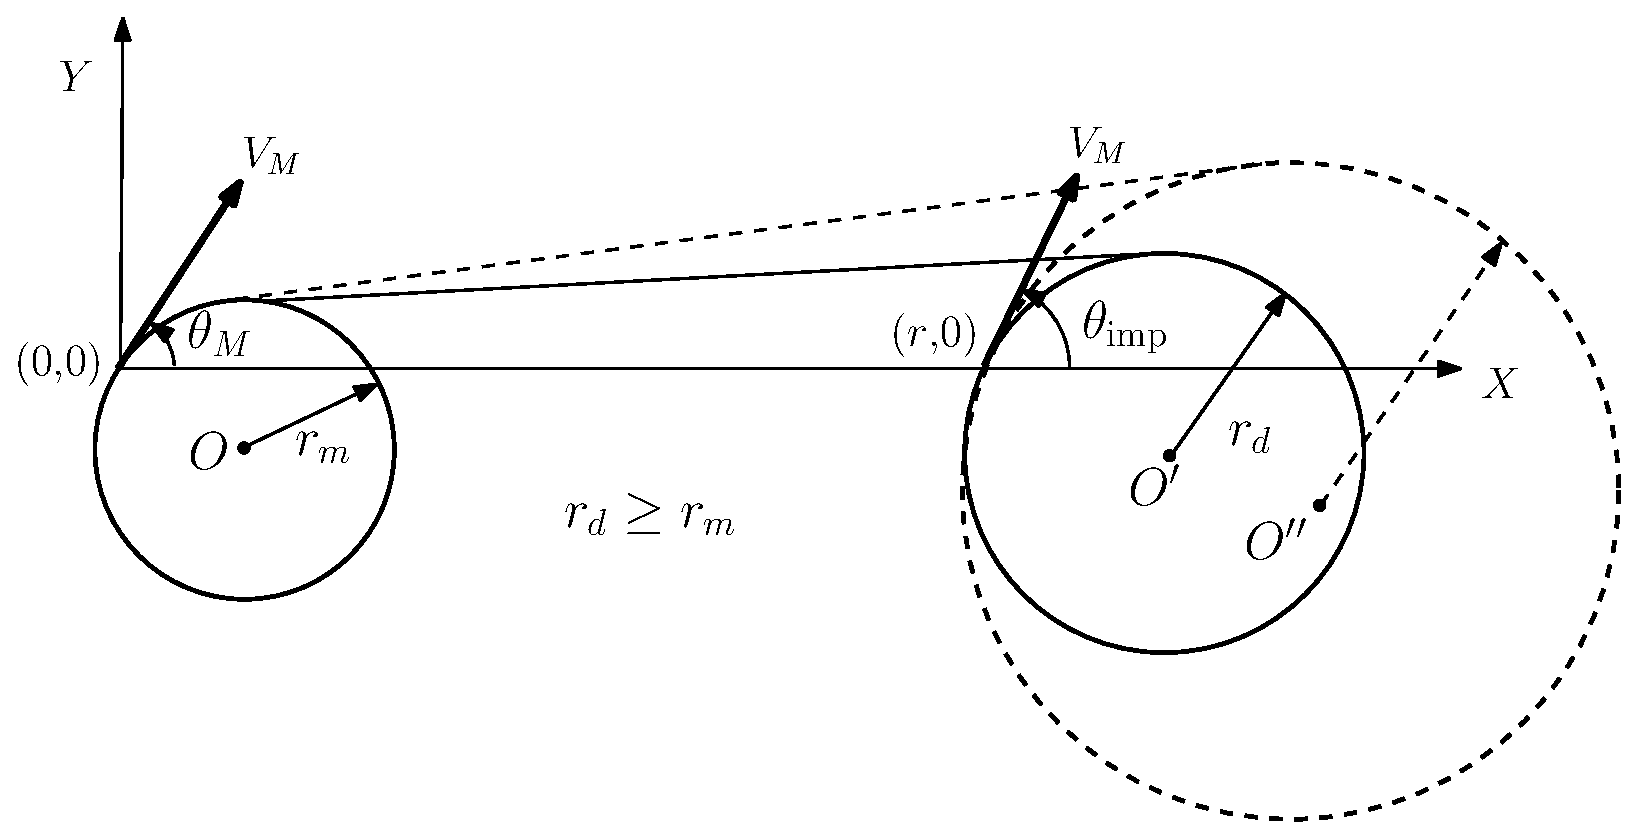
\includegraphics[width=\textwidth]{fig33.eps}
		\caption{Direct common tangent (DCT) path.}
		\label{fig:ch_DP_figdct}
	\end{subfigure}
	\caption{Dubins-like path geometry utilizing an \emph{outer} circle at the target location to satisfy simultaneous impact angle and unbounded impact time requirements.}
	\label{fig:ch_DP_outer_tct_dct}
\end{figure}

The primary geometric distinctions between TCT and DCT outer configurations are characterized by the velocity vector alignments along the vertical axis:
\begin{itemize}
    \item \textbf{Transverse Common Tangent (TCT):} Corresponds to engagement geometries where the $Y$-components of the interceptor's initial and final velocity vectors have \emph{opposite algebraic signs} ($\operatorname{sgn}(V_{y,0}) \neq \operatorname{sgn}(V_{y,f})$).
    \item \textbf{Direct Common Tangent (DCT):} Corresponds to engagement geometries where the initial and final velocity vectors lie in the same vertical half-plane ($\operatorname{sgn}(V_{y,0}) = \operatorname{sgn}(V_{y,f})$), i.e., both velocity vectors have positive $Y$-components (quadrants I and II) or both have negative $Y$-components (quadrants III and IV).
\end{itemize}

As evident from Figure \ref{fig:ch_DP_outer_tct_dct}, placing an outer circle at the target location eliminates circle-intersection limits. Consequently, no finite upper bound exists for the secondary radius ($r_d \in [r_m, \infty)$). As $r_d \to \infty$, the total path length increases continuously ($P(r_d) \to \infty$), allowing exact matching for arbitrarily large desired impact time values, $t^{\star}$.

Importantly, the fundamental structure of the lateral acceleration guidance command in \eqref{eq:ch_DP_open_loop_guidance} and its closed-loop state feedback counterpart in \eqref{eq:ch_DP_closed_loop_guidance} remain \emph{identical}. The piecewise-constant control command continues to demand exactly three discrete acceleration levels ($+a^{\max}, 0, -a^{\max}\frac{r_m}{r_d}$), provided that the design radius $r_d$ and switching lengths ($A_1, L_{\text{DCT}}, A_2$) are evaluated using the corresponding DCT/outer-circle geometric equations.
\subsection{Path Length Monotonicity}\label{subsec:ch_DP_monotonicity}

The fundamental property that enables precise numerical root-finding (such as bisection or Newton-Raphson methods) to obtain $r_d$ for a desired target impact time $t^\star$ is the monotonicity of the path length functions.

\begin{remark}[Path Length Monotonicity]\label{rem:ch_DP_monotonicity}
The path length $P(r_d)$ defined in \eqref{eq:ch_DP_total_path_length} is a strictly monotonically increasing function of $r_d$ over the interval $r_d \in [r_m, r_{\text{crit}}^{\text{TCT}}]$. Similarly, the mirrored path length $P'(r_d')$ defined in \eqref{eq:ch_DP_mirrored_path_length} is a strictly monotonically increasing function over $r_d' \in [r_m, \infty)$.
\end{remark}

The variation of total path length $P$ with respect to the designed turning radius $r_d$ for the TCT-based formulation is illustrated in Figure \ref{fig:ch_DP_lengthvsradius}.

\begin{figure}[!ht]
	\centering
	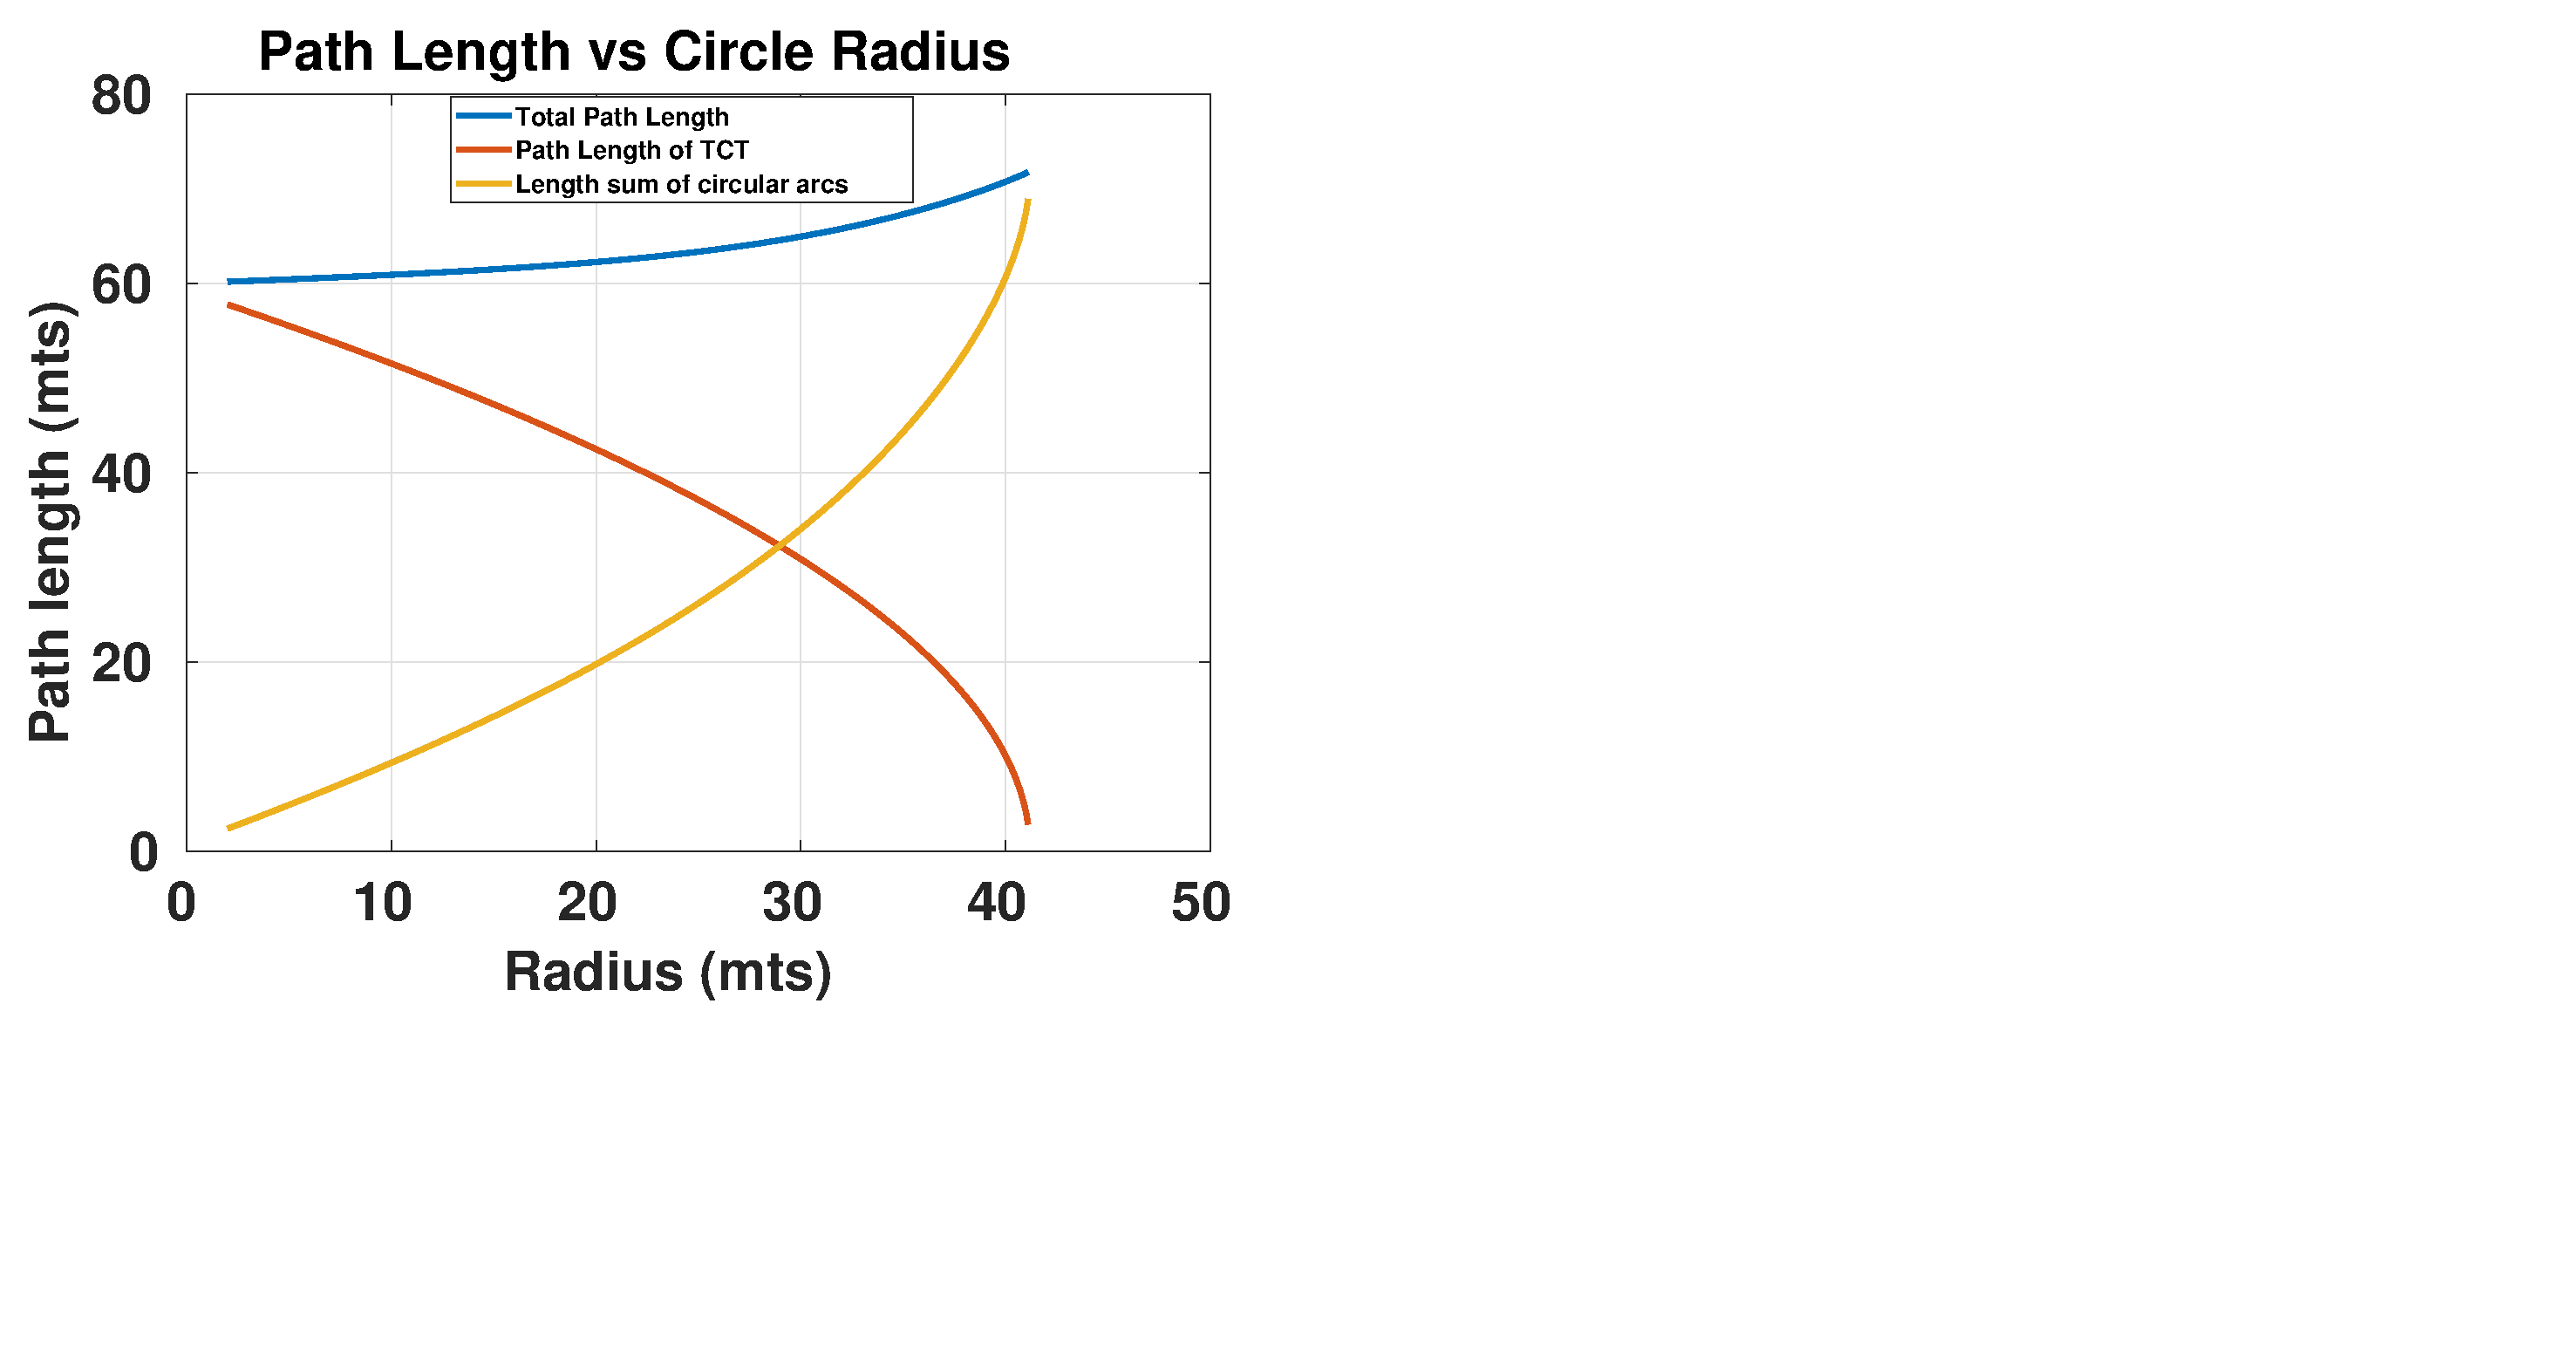
\includegraphics[trim={0cm 6cm 25cm 0cm},clip,scale=0.6]{5_Images/RadiusVsPathLength1.eps}
	\caption{Path length variation versus secondary turning radius $r_d \in [r_m, r_{\text{crit}}^{\text{TCT}})$.}
	\label{fig:ch_DP_lengthvsradius}
\end{figure}

Because $P(r_d)$ and $P'(r_d')$ are strictly monotonic and continuous, by the Intermediate Value Theorem \cite{rudin1964principles}, for any desired arrival time $t^\star \in [t_{\text{imp}}(r_m), t_{\text{imp}}(r_{\text{crit}}))$, there exists a unique secondary radius $r_d^\star$ satisfying $t_{\text{imp}}(r_d^\star) = t^\star$.
\section{Guidance Protocol and Implementation}\label{sec:ch_DP_guidance_law}
In Section \ref{sec:ch_DP_main_design}, we established the static spatial geometry of the Dubins-like path, determining the exact arc lengths $A_1$, $A_2$, common tangent length $L_{\text{TCT}}$, and secondary turning radius $r_d$ required to achieve the desired terminal approach angle $\theta_t$ and arrival time $t^{\star}$. However, physically executing this spatial trajectory requires converting static geometric parameters into a time-varying lateral acceleration command $a_M(t)$ that the autopilot can track dynamically.

In this section, we construct the open-loop guidance protocol and subsequently reformulate it into a robust, singularity-free closed-loop state feedback law.
\subsection{Mapping Spatial Geometry to Temporal Acceleration Demands}\label{subsec:ch_DP_spatial_to_temporal}

Because the interceptor operates at a constant forward velocity $V_M$, there exists a direct linear mapping between spatial progress along the path (arc length $s$) and temporal elapsed time ($t = s / V_M$). Each of the three distinct path segments synthesized in Section \ref{sec:ch_DP_main_design} corresponds to a dedicated time interval during which a constant lateral acceleration command is applied:

\begin{enumerate}
    \item \textbf{Phase 1: Initial Turning Segment ($0 \le t < t_1$):} To traverse arc $A_1$ on primary circle $C_1$ at minimum turn radius $r_m = V_M^2 / a^{\max}$, the interceptor demands maximum lateral acceleration:
    \begin{equation}\label{eq:ch_DP_phase1_accel}
        |a_M(t)| = \frac{V_M^2}{r_m} = a^{\max}.
    \end{equation}
    The duration of this initial reorientation phase is strictly given by $t_1 = A_1 / V_M$.
    
    \item \textbf{Phase 2: Straight-Line Cruise Segment ($t_1 \le t < t_1 + t_2$):} Along the Transverse Common Tangent $L_{\text{TCT}}$, the path curvature is zero ($\kappa = 0$). Consequently, the guidance command vanishes:
    \begin{equation}\label{eq:ch_DP_phase2_accel}
        a_M(t) = 0.
    \end{equation}
    The elapsed time spent along the straight tangent is $t_2 = L_{\text{TCT}} / V_M$.
    
    \item \textbf{Phase 3: Terminal Alignment Segment ($t_1 + t_2 \le t \le t_{\text{imp}}$):} To traverse arc $A_2$ on secondary circle $C_2$ at design radius $r_d$, the vehicle demands a reduced lateral acceleration:
    \begin{equation}\label{eq:ch_DP_phase3_accel}
        |a_M(t)| = \frac{V_M^2}{r_d} = a^{\max} \left( \frac{r_m}{r_d} \right) \le a^{\max}.
    \end{equation}
    The duration of this final turn is $t_3 = A_2 / V_M$, yielding the total time of flight $t_{\text{imp}} = t_1 + t_2 + t_3$.
\end{enumerate}
\subsection{Piecewise-Constant Open-Loop Guidance Command}\label{subsec:ch_DP_open_loop}

Combining the three temporal phases described in Section \ref{subsec:ch_DP_spatial_to_temporal}, the demanded lateral acceleration $a_M(t)$ is generated as a piecewise-constant function governed by two discrete switching instants:
\begin{equation}\label{eq:ch_DP_open_loop_guidance}
	a_M(t) = \begin{cases}
		a^{\max} \operatorname{sgn}(x), & \text{for } 0 \le t < t_1, \\
		0, & \text{for } t_1 \le t < t_1 + t_2, \\
		a^{\max} \left( \frac{r_m}{r_d} \right) \operatorname{sgn}(y), & \text{for } t_1 + t_2 \le t \le t_{\text{imp}},
	\end{cases}
\end{equation}
where $t_1 = A_1 / V_M$, $t_2 = L_{\text{TCT}} / V_M$, and $t_3 = A_2 / V_M$ (such that $t_{\text{imp}} = t_1 + t_2 + t_3$), $\operatorname{sgn}(\cdot)$ is the standard signum function, and $x, y \in \mathbb{R} \setminus \{0\}$ establish turn directionalities (clockwise versus counterclockwise) depending on whether a standard or mirrored TCT geometry is selected.

\begin{remark}[Actuator Feasibility and Energy Efficiency]\label{rem:ch_DP_acceleration_efficiency}
Because the secondary turn radius is constrained by $r_d \ge r_m$, the terminal acceleration magnitude strictly satisfies $|a_M(t)| = a^{\max} \frac{r_m}{r_d} \le a^{\max}$. The total $L_1$-norm acceleration energy expenditure across the engagement is:
\begin{equation}\label{eq:ch_DP_acceleration_energy}
	\|a_M\|_1 \coloneqq \int_0^{t_{\text{imp}}} |a_M(t)| \mathrm{d}t = \left( \frac{r_d t_1 + r_m t_3}{r_d} \right) a^{\max},
\end{equation}
yielding an average lateral acceleration requirement of $\bar{a}_M = \left( \frac{r_d t_1 + r_m t_3}{r_d t_{\text{imp}}} \right) a^{\max} < a^{\max}$, which is significantly lower than classical high-gain terminal guidance laws.
\end{remark}
\subsection{Singularity-Free Closed-Loop Feedback Implementation}\label{subsec:ch_DP_closed_loop}

While the open-loop guidance law \eqref{eq:ch_DP_open_loop_guidance} mathematically satisfies all boundary conditions in ideal simulation environments, pure open-loop execution is highly sensitive to external wind disturbances, target position uncertainty, and autopilot response lag. To provide robust tracking capability, open-loop law \eqref{eq:ch_DP_open_loop_guidance} is reformulated into a closed-loop feedback structure.

Rather than indexing control switches by elapsed time $t$ (which accumulates clock drift), the closed-loop feedback law is driven by the instantaneous cumulative arc length $S(t)$ traversed by the interceptor from its states:
\begin{equation}\label{eq:ch_DP_arc_length_state}
    S(t) \coloneqq \int_0^t V_M(\tau) \mathrm{d}\tau = \int_0^t \sqrt{\dot{x}_M^2(\tau) + \dot{y}_M^2(\tau)} \, \mathrm{d}\tau.
\end{equation}

Using arc-length progress $S(t)$ as the feedback metric, the closed-loop guidance protocol is formulated as:
\begin{equation}\label{eq:ch_DP_closed_loop_guidance}
	a_M(S) = \frac{a^{\max}}{2} \left[ \left( 1 + \operatorname{sgn}(A_1 - S) \right) \operatorname{sgn}(x) + \left( \frac{r_m}{r_d} \right) \left( 1 - \operatorname{sgn}(A_1 + L_{\text{TCT}} - S) \right) \operatorname{sgn}(y) \right].
\end{equation}

To eliminate high-frequency control chattering and actuator wear across the switching boundaries $S = A_1$ and $S = A_1 + L_{\text{TCT}}$, the discontinuous signum functions in \eqref{eq:ch_DP_closed_loop_guidance} are approximated using hyperbolic tangent smoothers:
\begin{equation}\label{eq:ch_DP_sigmoid_smoothing}
	\operatorname{sgn}(\Delta S) \approx \tanh\left( \frac{\Delta S}{\epsilon_b} \right),
\end{equation}
where $\epsilon_b > 0$ denotes a small user-defined boundary layer width governing transition smoothness.

\begin{remark}[Singularity Avoidance at High Heading Errors]\label{rem:ch_DP_singularity_free}
\leavevmode\par\noindent
Conventional impact-time guidance laws (such as \cite{harl2011impact}) contain $\sec \theta_M$ terms that singularize when the lead angle approaches $\pi/2$ ($\theta_M \approx 90^\circ$). Because protocol \eqref{eq:ch_DP_closed_loop_guidance} relies on global arc-length progress $S(t)$ rather than LOS rate division, it is completely singularity-free for all launch angles $\theta_M(0) \in (-\pi, \pi]$.
\end{remark}

\section{Numerical Simulation Results}\label{sec:ch_DP_simulations}
Numerical simulations were performed to evaluate the guidance framework under various engagement geometries. The interceptor operates at constant speed $V_M = 500\text{ m/s}$ with maximum acceleration capacity $a^{\max} = 400\text{ m/s}^2$ ($r_m = 625\text{ m}$). The initial range to the stationary target is $r(0) = 10,000\text{ m}$.

\subsection{Simultaneous Impact Angle and Time Control}

In the first test scenario, the initial heading angle is set to $\gamma_M(0) = 90^\circ$ ($\theta_M(0) = 90^\circ$), with desired approach angle $\theta_t = 45^\circ$ and required arrival time $t^{\star} = 22.0\text{ s}$. 

Solving $t_{\text{imp}}(r_d) = 22.0\text{ s}$ yields design radius $r_d = 4,400\text{ m}$, giving segment times $[t_1, t_2, t_3] = [2.389, 9.729, 9.909]\text{ s}$. Figures \ref{fig:ch_DP_sim1_trajs} and \ref{fig:ch_DP_sim1_accel} display the trajectory and smooth piecewise-constant lateral acceleration profile $a_M(t)$. The interceptor hits the target at exactly $t = 22.0\text{ s}$ with terminal angle $\gamma_M(t_{\text{imp}}) = 45.0^\circ$.

\begin{figure}[ht!]
	\centering
	\begin{subfigure}[b]{0.8\textwidth}
		\centering
		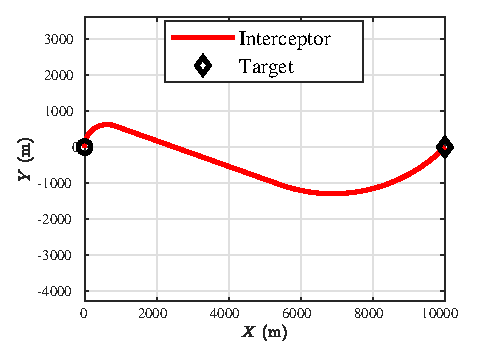
\includegraphics[width=\textwidth, keepaspectratio]{5_Images/trajakd.eps}
		\caption{Spatial engagement trajectory.}
		\label{fig:ch_DP_sim1_trajs}
	\end{subfigure}
	
	\vspace{1em}
	
	\begin{subfigure}[b]{0.8\textwidth}
		\centering
		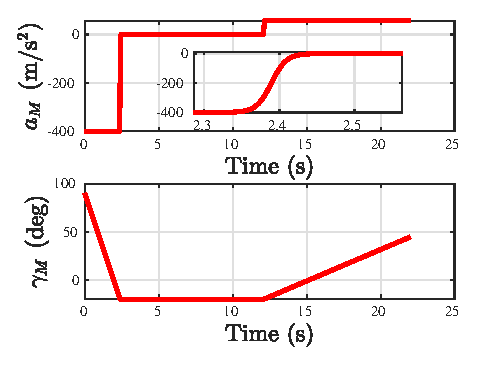
\includegraphics[width=\textwidth, keepaspectratio]{5_Images/amsigmakd.eps}
		\caption{Lateral acceleration $a_M(t)$ and flight path angle $\gamma_M(t)$.}
		\label{fig:ch_DP_sim1_accel}
	\end{subfigure}
	\caption{Target interception under TCT guidance with $\gamma_M(0) = 90^\circ$, desired approach angle $\theta_t = 45^\circ$, and terminal time $t^{\star} = 22.0\text{ s}$ ($r_d = 4,400\text{ m}$).}
	\label{fig:ch_DP_sim1_combined}
\end{figure}
\subsection{Arrival Time Variation via Design Radius $r_d$}

To demonstrate arrival time flexibility, Figure \ref{fig:ch_DP_sim2_radius_var} plots trajectories for a fixed approach angle $\theta_t = 45^\circ$ across varying design radii $r_d \in [r_m, r_{\text{crit}}^{\text{TCT}})$. Increasing $r_d$ expands the path length, smoothly shifting arrival times across $t_{\text{imp}} \in \{18.2\text{ s}, 22.0\text{ s}, 25.5\text{ s}\}$.

\begin{figure}[ht!]
	\centering
	\begin{subfigure}[b]{0.8\textwidth}
		\centering
		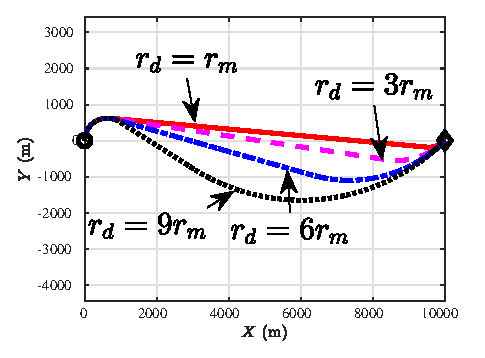
\includegraphics[width=\textwidth, keepaspectratio]{5_Images/traj_tct_compakd.eps}
		\caption{Trajectories for varying secondary radii $r_d$.}
		\label{fig:ch_DP_sim2_trajs}
	\end{subfigure}
	
	\vspace{1em}
	
	\begin{subfigure}[b]{0.8\textwidth}
		\centering
		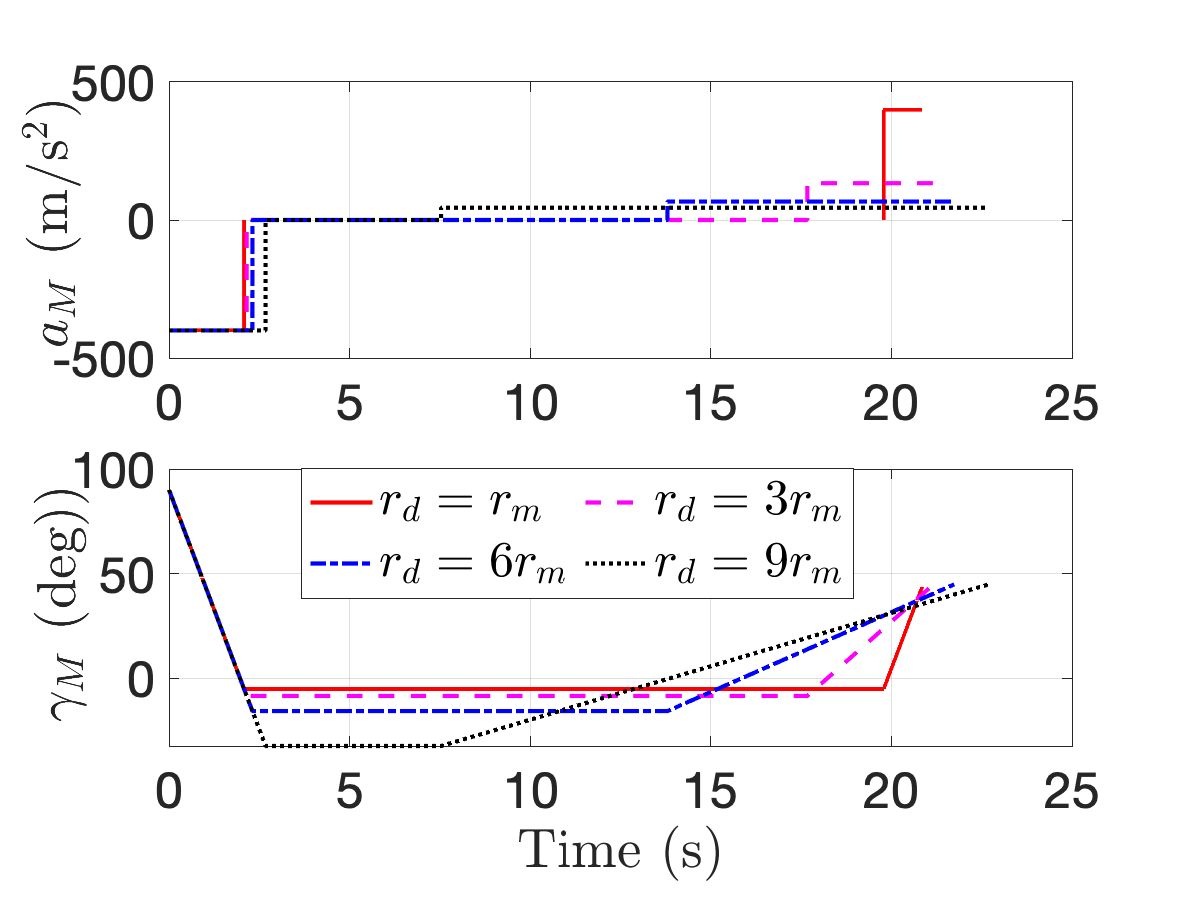
\includegraphics[width=\textwidth, keepaspectratio]{5_Images/amgammam_tct_compsrk.eps}
		\caption{Piecewise lateral acceleration profiles $a_M(t)$.}
		\label{fig:ch_DP_sim2_accel}
	\end{subfigure}
	\caption{Terminal arrival time tuning for $\theta_t = 45^\circ$ by adjusting secondary radius $r_d$.}
	\label{fig:ch_DP_sim2_radius_var}
\end{figure}

For extended arrival times ($t_{\text{imp}} \in \{60\text{ s}, 85\text{ s}, 100\text{ s}\}$), the mirrored TCT configuration ($C_2'$) is selected (Figure \ref{fig:ch_DP_sim3_outer}), validating unbounded arrival time capability.

\begin{figure}[ht!]
	\centering
	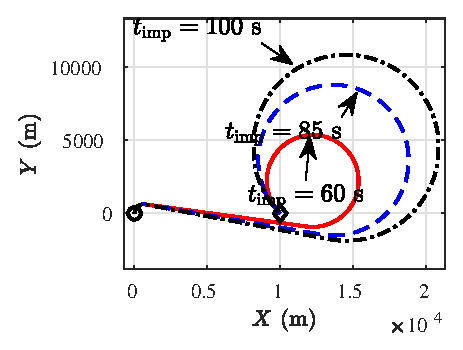
\includegraphics[width=0.85\textwidth, keepaspectratio]{5_Images/traj_out_tct1akd.eps}
	\caption{Large impact time trajectories ($t_{\text{imp}} \in \{60\text{ s}, 85\text{ s}, 100\text{ s}\}$) achieved using mirrored TCT geometry.}
	\label{fig:ch_DP_sim3_outer}
\end{figure}
\subsection{Comparative Evaluation with Existing Guidance Laws}
Figure \ref{fig:ch_DP_sim4_comparison} compares the proposed guidance protocol against two benchmark dual-constraint guidance laws: Zhang et al. \cite{Zhang2013} and Harl \& Willey \cite{harl2011impact}.

\begin{figure}[ht!]
	\centering
	\begin{subfigure}[b]{0.8\textwidth}
		\centering
		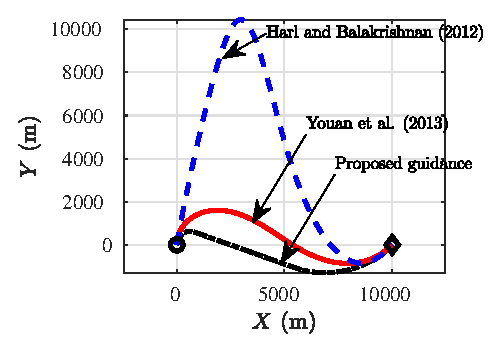
\includegraphics[width=\textwidth, keepaspectratio]{5_Images/traj_compakd.eps}
		\caption{Trajectory comparison.}
		\label{fig:ch_DP_sim4_trajs}
	\end{subfigure}
	
	\vspace{1em}
	
	\begin{subfigure}[b]{0.8\textwidth}
		\centering
		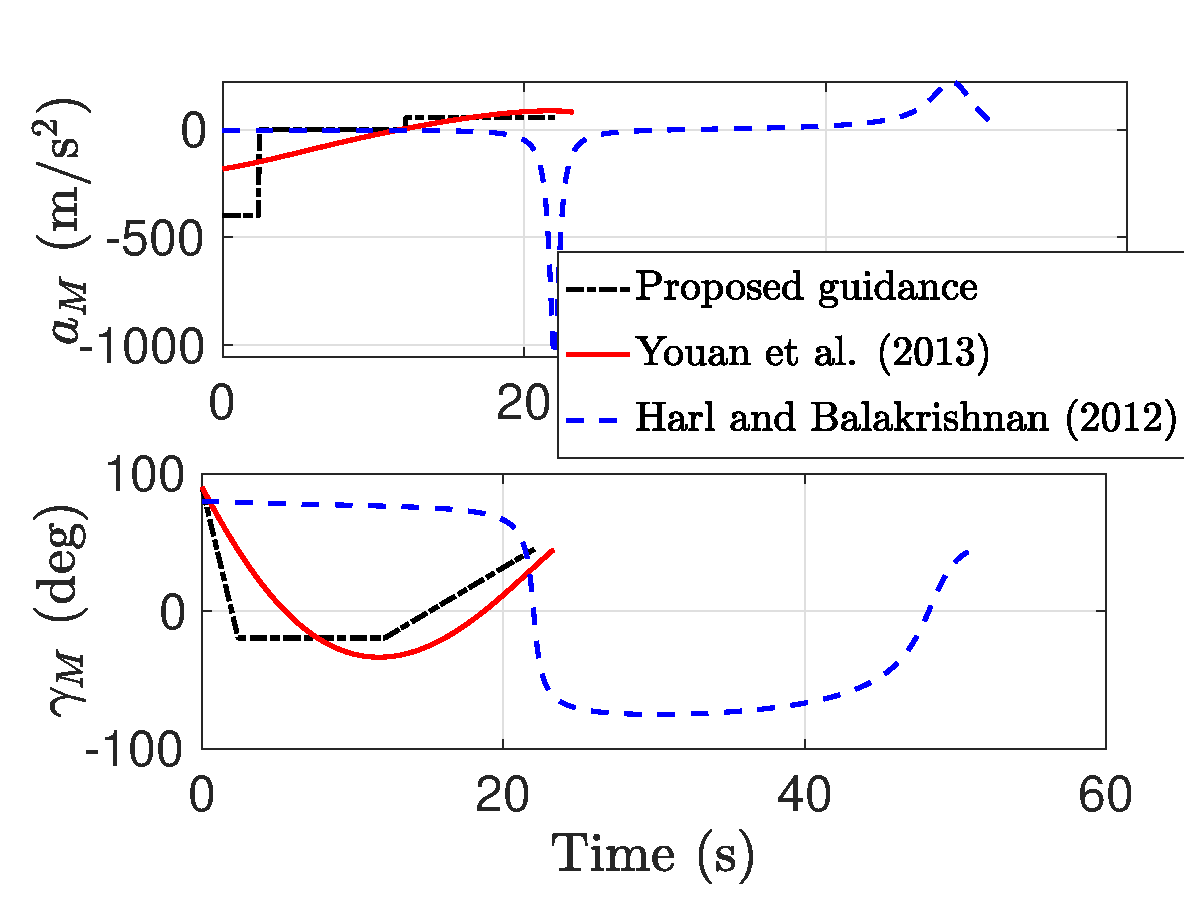
\includegraphics[width=\textwidth, keepaspectratio]{5_Images/am_comp_dubsrk.eps}
		\caption{Acceleration profile comparison.}
		\label{fig:ch_DP_sim4_accel}
	\end{subfigure}
	\caption{Performance comparison against existing guidance laws \cite{Zhang2013, harl2011impact} for $\theta_t = 45^\circ$ and $t^{\star} = 22.0\text{ s}$.}
	\label{fig:ch_DP_sim4_comparison}
\end{figure}
\begin{table}[ht!]
	\centering
	\caption{Comparative Guidance Performance Summary ($\theta_t = 45^\circ$, $t^{\star} = 22.0\text{ s}$)}
	\label{tab:ch_DP_comparison_table}
	\small
	\begin{tabularx}{\textwidth}{@{} >{\RaggedRight}X cccc @{}}
		\toprule
		\textbf{Guidance Method} & \textbf{Achieved } $t_{\text{imp}}$ \textbf{(s)} & \textbf{Achieved } $\theta_t$ & \textbf{Max } $|a_M|$ \textbf{(m/s}$^2$\textbf{)} & $\|a_M\|_1$ \textbf{(m/s}$^2$\textbf{)} \\
		\midrule
		Zhang et al. \cite{Zhang2013} & 23.35 & $45.0^\circ$ & 382.1 & 1,759.4 \\
		Harl \& Willey \cite{harl2011impact} ($\theta_M=80^\circ$) & 51.63 & $45.0^\circ$ & 400.0 & 2,401.9 \\
		\textbf{Proposed Dubins Protocol} & \textbf{22.00} & $\mathbf{45.0^\circ}$ & \textbf{400.0} & \textbf{1,517.3} \\
		\bottomrule
	\end{tabularx}
\end{table}
As summarized in Table \ref{tab:ch_DP_comparison_table}, Zhang's law \cite{Zhang2013} exceeds the desired arrival time ($23.35\text{ s}$ vs. $22.0\text{ s}$). Harl's law \cite{harl2011impact} singularizes at $\theta_M = 90^\circ$ and yields an erroneous arrival time of $51.63\text{ s}$ even when launched at $\theta_M = 80^\circ$. In contrast, the proposed Dubins protocol meets both terminal constraints precisely ($t_{\text{imp}} = 22.00\text{ s}, \theta_t = 45.0^\circ$) while consuming the lowest total acceleration energy ($\|a_M\|_1 = 1,517.3\text{ m/s}^2$).

\section{Summary}\label{sec:ch_DP_summary}
In this chapter, an open-loop and equivalent closed-loop trajectory planning framework was synthesized using Dubins-like path geometry to achieve simultaneous terminal approach angle $\theta_t$ and terminal arrival time $t_{\text{imp}}$ constraints against stationary targets. The primary conclusions are:
\begin{itemize}
    \item \textbf{Implementable Acceleration Profile:} The proposed guidance protocol demands piecewise-constant lateral acceleration across three discrete level acceleration profile ($+a^{\max}, 0, -a^{\max} \frac{r_m}{r_d}$), eliminating high-order polynomial computation and preventing actuator saturation.
    \item \textbf{Flexible Arrival Time Tuning:} Introducing variable secondary turn radius $r_d \ge r_m$ allows exact terminal time matching, while mirrored circle geometry ($C_2'$) renders achievable arrival times unbounded above.
    \item \textbf{Singularity-Free Closed-Loop Execution:} Distance-based closed-loop feedback \eqref{eq:ch_DP_closed_loop_guidance} with hyperbolic tangent smoothing removes trigonometric singularities at large lead angles ($\theta_M \approx 90^\circ$).
\end{itemize}

\vspace{0.5em}
\noindent %\textbf{Transition to Chapter 6:}\\
While Chapter \ref{ch:Dubins_Path} solved single-agent trajectory generation under nonholonomic constraints and terminal arrival time matching, coordinating multi-agent swarms in spatial pursuit scenarios requires integrating single-vehicle path geometry with collective team interception dynamics. 

Chapter \ref{ch:Spiral_Path} extends these geometric concepts to multi-agent swarm pursuit, formulating Archimedean spiral-based path synthesis and spatial rendezvous strategies for cooperative multi-interceptor teams.

%\chapter{Trajectory planning using Dubins-like paths with approach angle and terminal time constraints}\label{ch:5_Dubins_Path}










%\chapter{Spiral–Based Guidance Law and Multi-Agent Coordination}\label{ch:Spiral_Path}
\chapter[Spiral-Based Guidance Laws and Multi-Agent Spatial Coordination]{Spiral-Based Guidance Laws and Multi-Agent Spatial Coordination}\label{ch:Spiral_Path}
\section{Introduction and Motivation}\label{sec:ch_sp_intro}
In Chapter \ref{ch:Dubins_Path}, we formulated nonholonomic single-agent trajectory planning using Dubins-like geometric paths, demonstrating how adjusting a secondary turn radius $r_d$ satisfies simultaneous terminal approach angle and time-of-arrival constraints. While Dubins trajectories provide a minimal-length piecewise-constant acceleration framework, their discrete curvature jumps ($\kappa \in \{+1/r_m, 0, -1/r_d\}$) introduce jump discontinuities in the lateral acceleration profile. In high-speed atmospheric vehicles, agile robotic swarms, or guided precision interceptors, such step acceleration demands can excite unmodeled autopilot lag, induce mechanical chatter, or cause actuator saturation.

To achieve continuous curvature trajectories without discontinuities in lateral acceleration, \textbf{spiral-based path geometries} present a powerful alternative. Impact-angle-constrained guidance plays a pivotal role in modern cooperative engagements, where arriving at a target along specific spatial vectors maximizes warhead penetration, aligns directional sensors, or bypasses defensive countermeasure zones. Classical guidance laws—such as Pure Pursuit (PP) \cite{SHNEYDOR199847}, Deviated Pure Pursuit (DPP), and Proportional Navigation Guidance (PNG) \cite{SHNEYDOR1998101}— guarantee target interception but do not inherently enforce terminal impact angle constraints without demanding infinite terminal acceleration. Modified state-dependent Riccati equation (SDRE) laws \cite{ratnoo2009SDRE} and biased PNG schemes \cite{Kim2013} enforce impact angle constraints, but typically induce severe acceleration spikes near interception. Polynomial guidance approaches \cite{kim2013time} enforce boundary conditions but require rigid pre-computed trajectories that degrade under external wind perturbations or autopilot lags.

Generalized Archimedean spirals provide an attractive alternative: their polar geometry inherently embeds the desired terminal approach angle $\zeta$, while providing continuous, smooth curvature modulation throughout the engagement. However, existing spiral-based guidance schemes (e.g., \cite{tripathy2019archimedean}, \cite{mishra2024spiral}) operate under an unexamined assumption: they assume the initial geometric scaling parameter $\alpha_0$ yields a physically realizable path. If the initial launch geometry dictates a scaling factor below a critical reference threshold ($\alpha_0 < \alpha_{\text{ref}}$), the demanded lateral acceleration exceeds the physical actuator limits ($|a_p(t)| > a_{\max}$), causing catastrophic control saturation, leading to unacceptable miss-distances.

To overcome these challenges, this chapter presents a \emph{two-phase adaptive spiral guidance framework} that guarantees impact angle satisfaction while respecting strict physical actuator limits ($|a_p(t)| \le a_{\max}$). Furthermore, we extend this framework to multi-agent spatial coordination, using consensus in the spiral scaling parameter $\alpha$, over directed graphs to achieve distributed, sector-allocated coordinated interception. 

Although the framework presented in this chapter overcomes key physical and geometric limitations of classic Dubins-like strategies—extending them to multi-agent cooperative interception—we deliberately relax the requirement of strict simultaneous interception. Consequently, explicit terminal impact time constraints are not imposed, allowing the guidance strategy to prioritize angular sector alignment, actuator feasibility, and computational efficiency.

\subsection*{Summary of Chapter Contributions}
The primary analytical and algorithmic contributions of this chapter are:
\begin{enumerate}
    \item \textbf{Curvature Feasibility Analysis:} We derive exact closed-form expressions for the maximum curvature $\kappa_{\max} = f(\beta)/\alpha$ of generalized Archimedean spirals, establishing a sharp physical feasibility threshold $\alpha_{\text{ref}} \coloneqq v_p^2 f(\beta) / a_{\max}$.
    \item \textbf{Two-Phase Adaptive Scaling Control:} We formulate a two-phase guidance law that proactively adapts the scaling factor $\alpha(t) \to \alpha_{\text{ref}}$ during Phase 1 whenever $\alpha_0 < \alpha_{\text{ref}}$, eliminating lateral acceleration saturation before transitioning to Phase 2 terminal angle tracking.
    \item \textbf{Prescribed-Time Robust Error Suppression:} We integrate prescribed-time sliding mode control components into the adaptive spiral dynamics, proving finite-time error convergence $e(t) \to 0$ as $t \to T^*$ despite bounded process noise.
    \item \textbf{Directed Graph Multi-Agent Coordination:} We extend the single-agent framework to multi-agent swarms by executing directed chain consensus over the spiral parameter vector $\boldsymbol{\alpha}$, achieving synchronized, sector-allocated directional cooperative attacks across heterogeneous vehicle fleets.
\end{enumerate}
\section{Engagement Geometry and Kinematics}\label{sec:ch_sp_kinematics}
Consider the planar engagement geometry shown in Figure \ref{fig:ch_sp_eng_geometry}, where a pursuer (interceptor) engages a stationary target located at the origin $(x_t, y_t) = (0,0)$. The pursuer travels at constant speed $v_p > 0$ with heading angle $\gamma_p(t)$. Its control input is the lateral acceleration $a_p(t) \in \mathbb{R}$, subject to strict actuator saturation limits $|a_p(t)| \le a_{\max}$.

\begin{figure}[!ht]
	\centering
	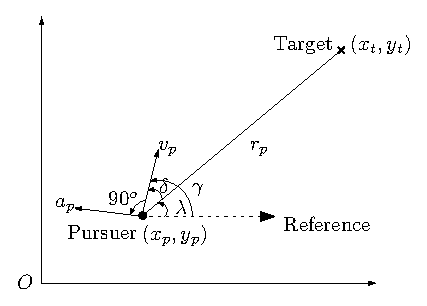
\includegraphics[width=0.75\textwidth, keepaspectratio]{6_Images/Eng_geom.eps}
	\caption{Planar engagement geometry between a pursuer and a stationary target in polar coordinates $(r_p, \lambda_p)$.}
	\label{fig:ch_sp_eng_geometry}
\end{figure}

The Cartesian kinematic equations of motion are:
\begin{equation}\label{eq:ch_sp_cartesian_kinematics}
	\dot{x}_p(t) = v_p \cos \gamma_p(t), \quad \dot{y}_p(t) = v_p \sin \gamma_p(t).
\end{equation}

To simplify geometric trajectory tracking, define the polar state variables:
\begin{itemize}
	\item $r_p(t) \coloneqq \sqrt{(x_t - x_p)^2 + (y_t - y_p)^2}$ : Range to target
	\item $\lambda_p(t) \coloneqq \operatorname{atan2}(y_t - y_p, x_t - x_p)$ : Line-of-sight (LOS) angle
	\item $\delta_p(t) \coloneqq \gamma_p(t) - \lambda_p(t)$ : Lead angle (look angle)
\end{itemize}

The nonholonomic engagement dynamics in polar coordinates are:
\begin{align}
	\dot{r}_p(t) &= -v_p \cos \delta_p(t) \label{eq:ch_sp_r_dot} \\
	r_p(t) \dot{\lambda}_p(t) &= -v_p \sin \delta_p(t) \label{eq:ch_sp_lambda_dot} \\
	\dot{\gamma}_p(t) &= \frac{a_p(t) + n(t)}{v_p}, \label{eq:ch_sp_gamma_dot}
\end{align}
where $n(t) \in \mathbb{R}$ represents bounded external process noise or wind disturbances ($|n(t)| \le N_0$).
In accordance with the physical constraints detailed in Section~\ref{sec:ch_DP_probform}, the commanded lateral acceleration is strictly bounded by $|a_M(t)| \le a^{\max}$ to avoid actuator saturation. Furthermore, the terminal boundary conditions are synthesized to meet the desired approach orientation $\theta_t$ as defined in Definition~\ref{def:ch_DP_impact_angle} and desired impact time as defined in ~\ref{def:ch_DP_impact_time}.
\begin{problem}\label{prob:ch_sp_main_problem}
Given an initial state configuration $\mathbf{x}(0) = [r_p(0), \lambda_p(0), \gamma_p(0)]^T$, constant flight speed $v_p$, maximum acceleration limit $a_{\max}$, and desired terminal approach angle $\zeta$, synthesize a continuous lateral acceleration guidance law $a_p(t)$ such that:
\begin{enumerate}
    \item \textbf{Target Interception:} The pursuer reaches the origin at terminal time $t_f$, satisfying $\lim_{t \to t_f} r_p(t) = 0$.
    \item \textbf{Impact Angle Satisfaction:} The velocity vector aligns precisely with the approach angle at interception: $\lim_{t \to t_f} \lambda_p(t) = \zeta$.
    \item \textbf{Actuator Feasibility:} The lateral acceleration strictly obeys the physical bound $|a_p(t)| \le a_{\max}$ for all $t \in [0, t_f]$.
\end{enumerate}
\end{problem}
\section{Archimedean Spiral Trajectory Framework}\label{sec:ch_sp_spiral_framework}
\leavevmode\par\noindent
To satisfy Problem \ref{prob:ch_sp_main_problem} without involving high-order polynomial calculations, or discontinuous step acceleration commands, we formulate trajectory generation using a generalized Archimedean spiral geometry.
\subsection{Geometric Parameterization and Chief Merits of Proposed Strategy}\label{subsec:ch_sp_spiral_def}

We parameterize the path of the pursuer in polar space $(r, \lambda)$ around the generalized Archimedean spiral:
\begin{equation}\label{eq:ch_sp_spiral_def}
	r(\lambda) = \alpha (\lambda - \zeta)^\beta, \quad \text{for } \lambda \ge \zeta,
\end{equation}
where $\zeta$ is the designated terminal impact angle, $\beta \in (0, 1]$ is a fixed geometric shape exponent, and $\alpha > 0$ is the spatial scaling parameter.

This parameterization introduces two fundamental geometric properties for guidance of nonholonomic vehicles which are very appealing:

\begin{enumerate}
    \item \textbf{Implicit Terminal Angle Alignment:} As relative range vanishes ($r \to 0$), the polar angle asymptotically approaches the target angle ($\lambda \to \zeta$). Because the tangent to spiral \eqref{eq:ch_sp_spiral_def} aligns with $\zeta$ at the origin, terminal impact angle satisfaction ($\lambda_p(t_f) = \zeta$) is intrinsically embedded into the spatial geometry, eliminating the need for high-gain terminal corrective steering.
    
    \item \textbf{Zero Terminal Acceleration Demand:} The geometry of the spiral \eqref{eq:ch_sp_spiral_def} dictates that path curvature $\kappa(\lambda)$ approaches zero as $\lambda \to \zeta$. Consequently, the commanded lateral acceleration $a_p = v_p^2 \kappa$ vanishes naturally at interception ($a_p(t_f) = 0$), thus avoiding terminal control saturation and autopilot chattering.
\end{enumerate}
\subsection{Path Curvature Analysis and Critical Feasibility Threshold}\label{subsec:ch_sp_curvature_analysis}

While the spiral geometry inherently satisfies terminal angle constraints, its physical realizability depends on whether the required path curvature exceeds the vehicle's turn capability ($a_{\max} / v_p^2$) or not. 

The path curvature $\kappa(\lambda)$ of a polar curve $r(\lambda)$ is governed by the classical relation:
\begin{equation}\label{eq:ch_sp_kappa_general_formula}
	\kappa(\lambda) = \frac{\big|r^2 + 2(r')^2 - r r''\big|}{\left( r^2 + (r')^2 \right)^{3/2}},
\end{equation}
where $r' \coloneqq \frac{\mathrm{d}r}{\mathrm{d}\lambda}$ and $r'' \coloneqq \frac{\mathrm{d}^2 r}{\mathrm{d}\lambda^2}$.

Differentiating parameterization \eqref{eq:ch_sp_spiral_def} with respect to $\lambda$ yields:
\begin{equation}\label{eq:ch_sp_spiral_derivatives}
    r' = \alpha \beta (\lambda - \zeta)^{\beta-1}, \quad r'' = \alpha \beta (\beta-1) (\lambda - \zeta)^{\beta-2}.
\end{equation}

Defining the angular offset $\theta \coloneqq \lambda - \zeta > 0$, substituting $r(\theta) = \alpha \theta^\beta$ and its derivatives \eqref{eq:ch_sp_spiral_derivatives} into \eqref{eq:ch_sp_kappa_general_formula} gives:
\begin{align}\label{eq:ch_sp_kappa_explicit_derivation}
	\kappa(\theta) &= \frac{\left| \alpha^2 \theta^{2\beta} + 2 \alpha^2 \beta^2 \theta^{2\beta-2} - \alpha^2 \beta(\beta-1) \theta^{2\beta-2} \right|}{\left( \alpha^2 \theta^{2\beta} + \alpha^2 \beta^2 \theta^{2\beta-2} \right)^{3/2}} \nonumber \\
	&= \frac{\alpha^2 \theta^{2\beta-2} \left| \theta^2 + \beta^2 + \beta \right|}{\alpha^3 \theta^{3\beta-3} \left( \theta^2 + \beta^2 \right)^{3/2}} \nonumber \\
	&= \frac{1}{\alpha} \cdot \frac{\theta^{1-\beta} (\beta^2 + \beta + \theta^2)}{(\beta^2 + \theta^2)^{3/2}}.
\end{align}

We isolate the dimensionless, scale-independent shape curvature function $f(\beta, \theta)$:
\begin{equation}\label{eq:ch_sp_f_beta_theta_def}
    f(\beta, \theta) \coloneqq \frac{\theta^{1-\beta} (\beta^2 + \beta + \theta^2)}{(\beta^2 + \theta^2)^{3/2}}, \implies \kappa(\theta) = \frac{f(\beta, \theta)}{\alpha}.
\end{equation}

To find the peak curvature along the trajectory, we differentiate $f(\beta, \theta)$ with respect to $\theta$ and solve $\frac{\partial f}{\partial \theta} = 0$, which yields the critical angular offset $\theta^*$:
\begin{equation}\label{eq:ch_sp_critical_theta}
    \theta^* = \sqrt{\sqrt{3\beta^2+1} - 1 - \beta^2}.
\end{equation}

Evaluating $f(\beta) \coloneqq \max_\theta f(\beta, \theta) = f(\beta, \theta^*)$ yields the maximum shape curvature constant:
\begin{equation}\label{eq:ch_sp_f_beta_max}
	f(\beta) = \frac{\sqrt{3\beta^2+1} + \beta - 1}{\left( \sqrt{3\beta^2+1} - 1 - \beta^2 \right)^{\frac{\beta-1}{2}} \left( \sqrt{3\beta^2+1} - 1 \right)^{3/2}}.
\end{equation}

Consequently, the peak curvature $\kappa_{\max}$ experienced along an Archimedean spiral trajectory is inversely proportional to the spatial scaling parameter $\alpha$:
\begin{equation}\label{eq:ch_sp_kappa_max}
	\kappa_{\max} = \frac{f(\beta)}{\alpha}.
\end{equation}

Since commanded lateral acceleration is related to curvature via $a_{\text{cmd}} = v_p^2 \kappa$, the maximum acceleration required to track the spiral is:
\begin{equation}\label{eq:ch_sp_acmd_max}
    a_{\max, \text{cmd}} = \frac{v_p^2 f(\beta)}{\alpha}.
\end{equation}

The variation of path curvature $\kappa(\theta)$ across different scaling values $\alpha$ for a fixed shape exponent $\beta = 0.5$ is illustrated in Figure \ref{fig:ch_sp_curv_vs_angle}.

\begin{figure}[!ht]
	\centering
	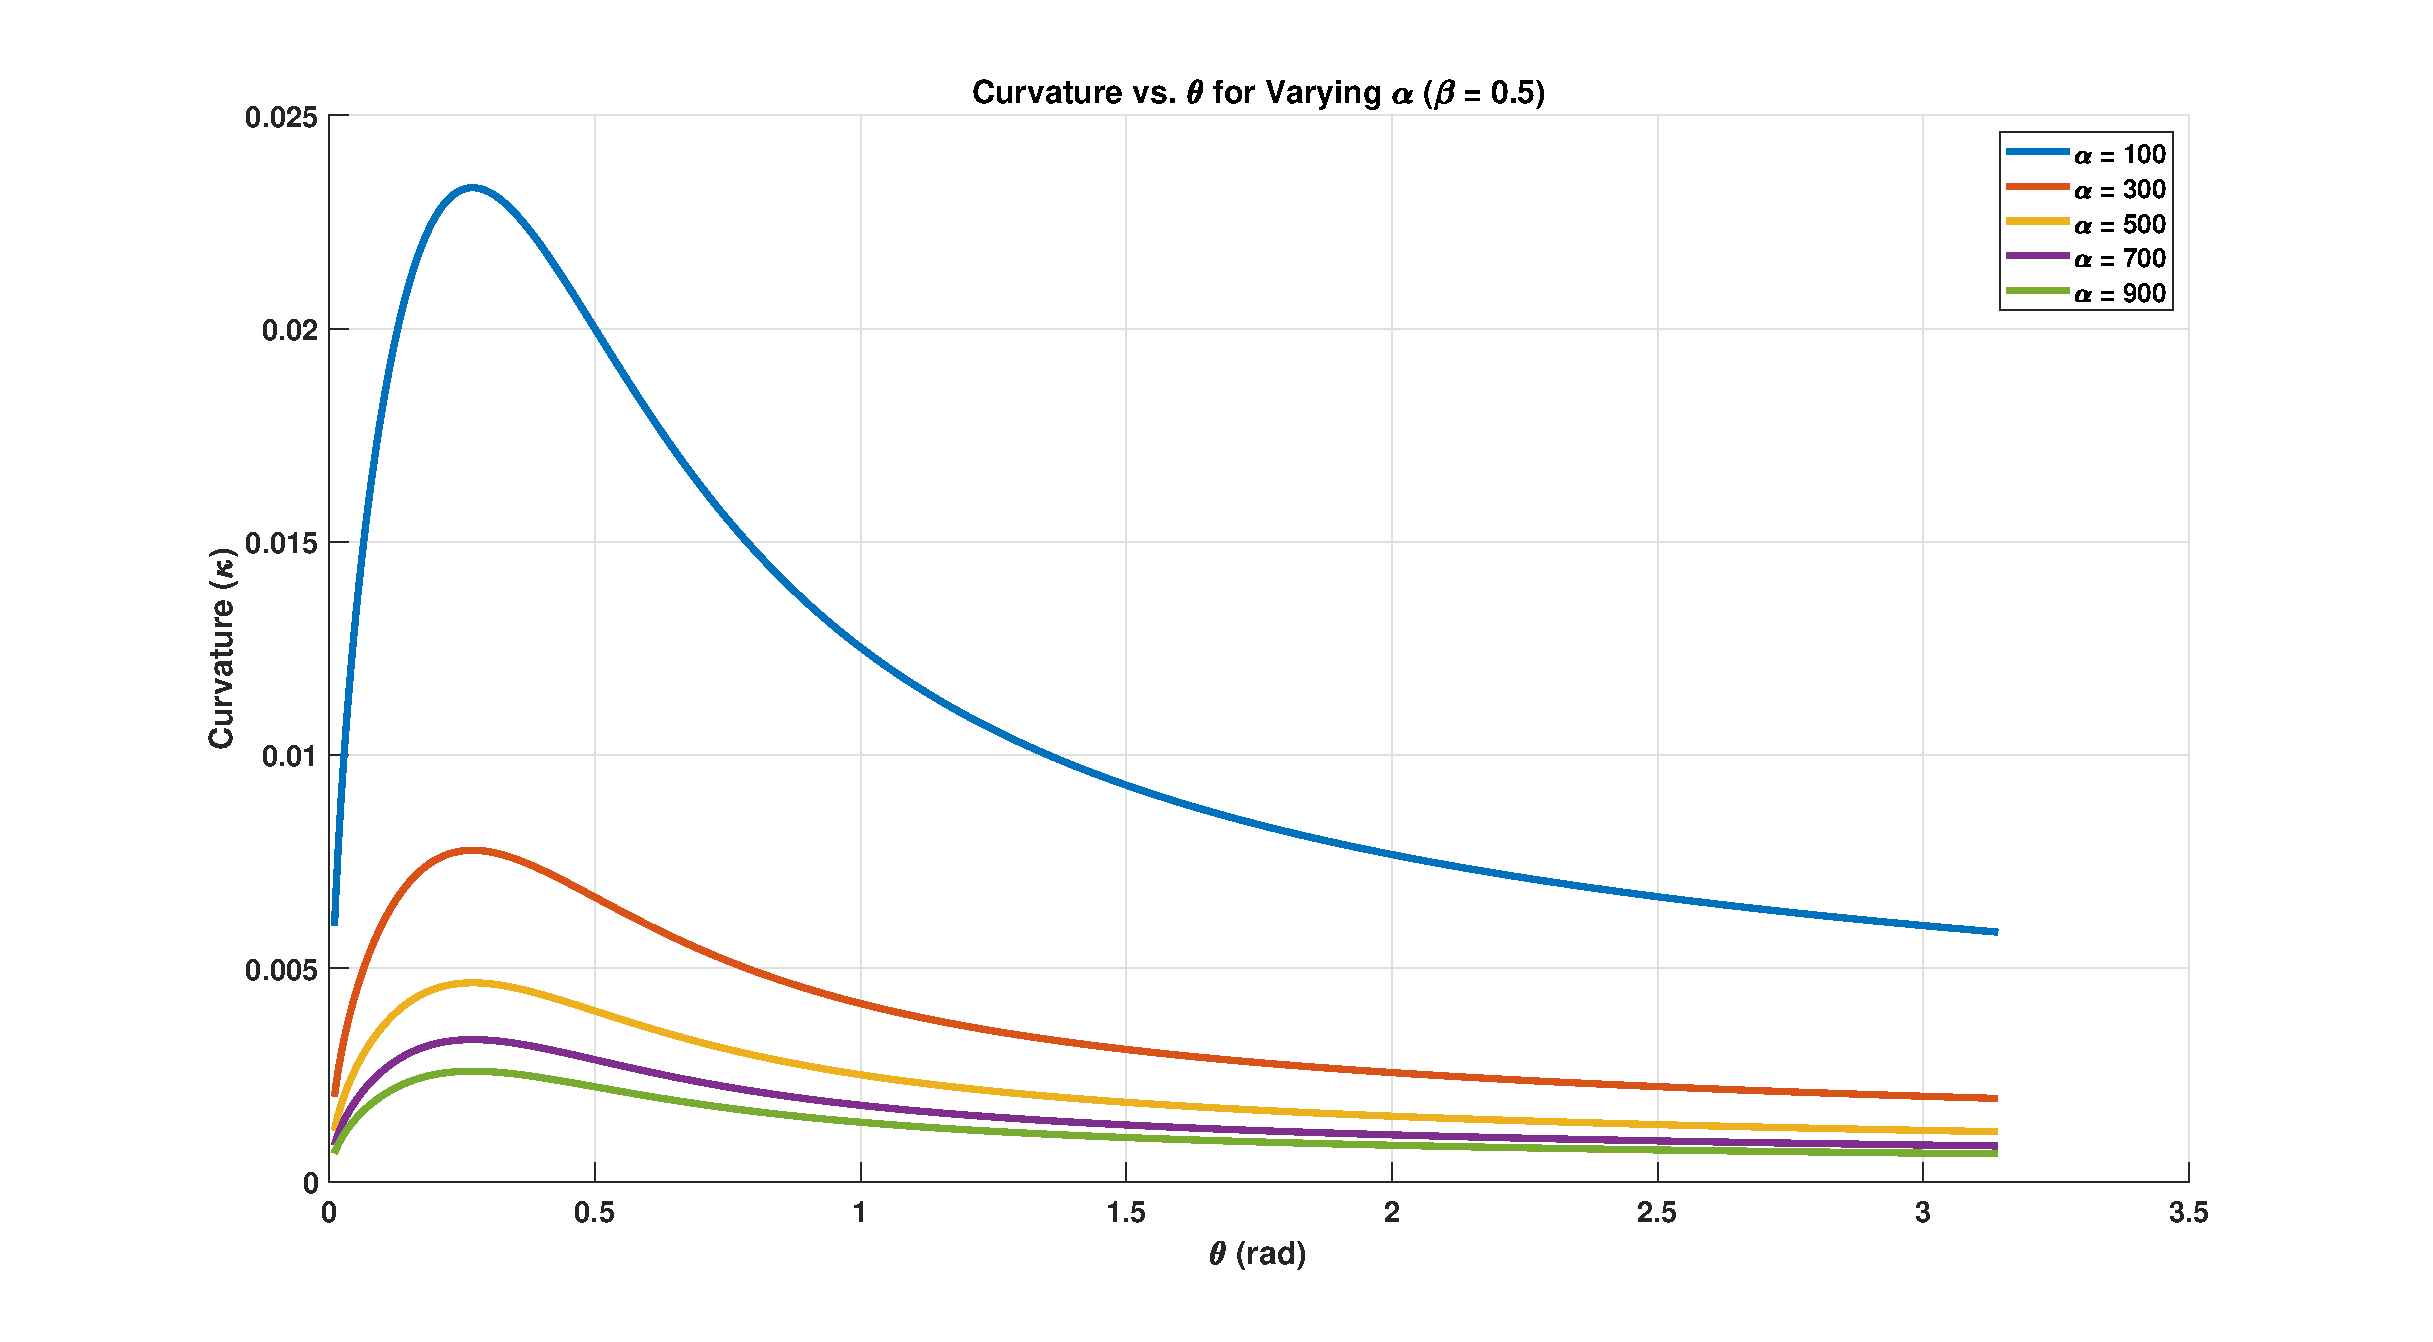
\includegraphics[width=0.75\textwidth]{6_Images/CurvVsAngle_FixedBeta_VaryingAlpha.eps}
	\caption{Path curvature $\kappa(\theta)$ versus angular offset $\theta = \lambda - \zeta$ for fixed exponent $\beta = 0.5$ across varying scaling factors $\alpha$. Smaller values of $\alpha$ significantly amplify peak trajectory curvature.}
	\label{fig:ch_sp_curv_vs_angle}
\end{figure}

\subsection{Physical Infeasibility of Unadapted Spiral Guidance}\label{subsec:ch_sp_infeasibility_proof}
To guarantee that the commanded lateral acceleration strictly respects actuator limits ($a_{\max, \text{cmd}} \le a_{\max}$), the scaling parameter $\alpha$ must satisfy $\alpha \ge \alpha_{\text{ref}}$, where the critical physical reference threshold $\alpha_{\text{ref}}$ is defined as:
\begin{equation}\label{eq:ch_sp_alpha_ref}
	\alpha_{\text{ref}} \coloneqq \frac{v_p^2 f(\beta)}{a_{\max}}.
\end{equation}

In standard unadapted spiral guidance laws (e.g., \cite{mishra2024spiral}), the scaling parameter $\alpha_0$ is statically computed from initial launch conditions:
\begin{equation}\label{eq:ch_sp_initial_alpha}
    \alpha_0 = \frac{r_p(0)}{\big(\lambda_p(0) - \zeta\big)^\beta}.
\end{equation}

Because initial range $r_p(0)$ and launch angles are dictated by arbitrary engagement geometry rather than actuator constraints, $\alpha_0$ frequently falls below the critical threshold ($\alpha_0 < \alpha_{\text{ref}}$). When $\alpha_0 < \alpha_{\text{ref}}$, the peak curvature demand exceeds $a_{\max} / v_p^2$, driving the actuators into saturation.

Figure \ref{fig:ch_sp_kushagra_breakdown} illustrates the catastrophic control breakdown that occurs under unadapted spiral guidance when $\alpha_0 < \alpha_{\text{ref}}$. Actuator saturation ($|a_p| = 30g$) prevents the pursuer from following the nominal spiral, causing large miss distances and trajectory degradation.

\begin{figure}[!ht]
	\centering
	\begin{subfigure}[b]{0.7\textwidth}
		\centering
		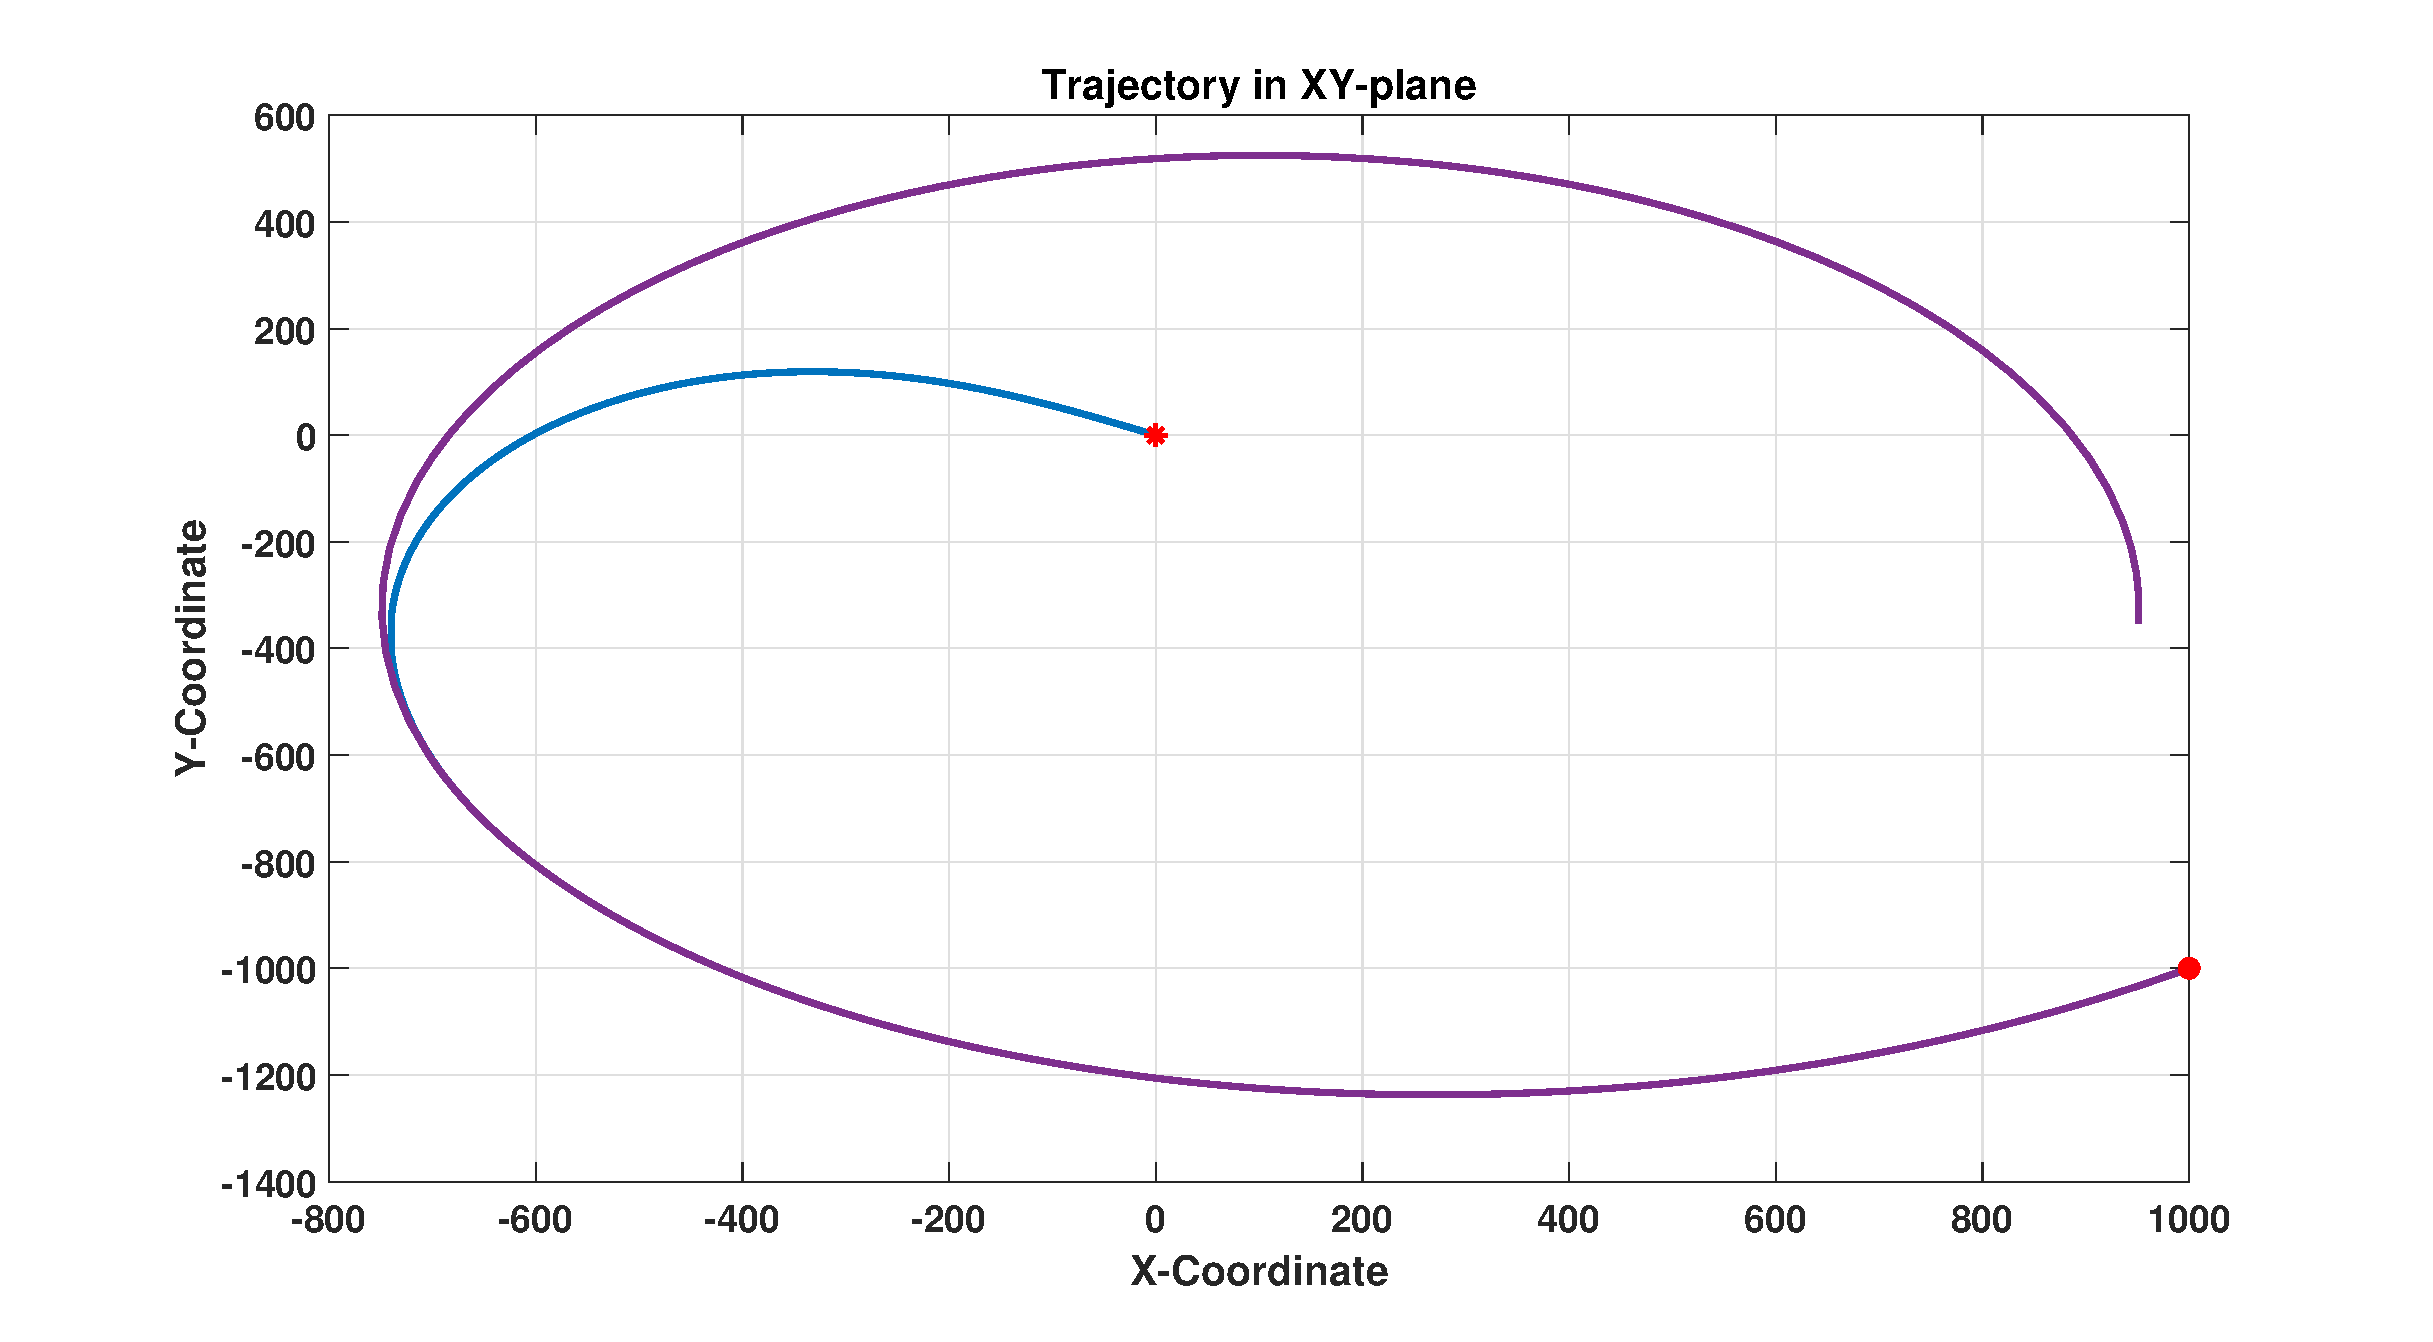
\includegraphics[width=\textwidth]{6_Images/Trajectory_Kushagra.eps}
		\caption{Interception trajectories with and without acceleration bounds.}
		\label{fig:ch_sp_kushagra_traj}
	\end{subfigure}
	\hfill
	\begin{subfigure}[b]{0.7\textwidth}
		\centering
		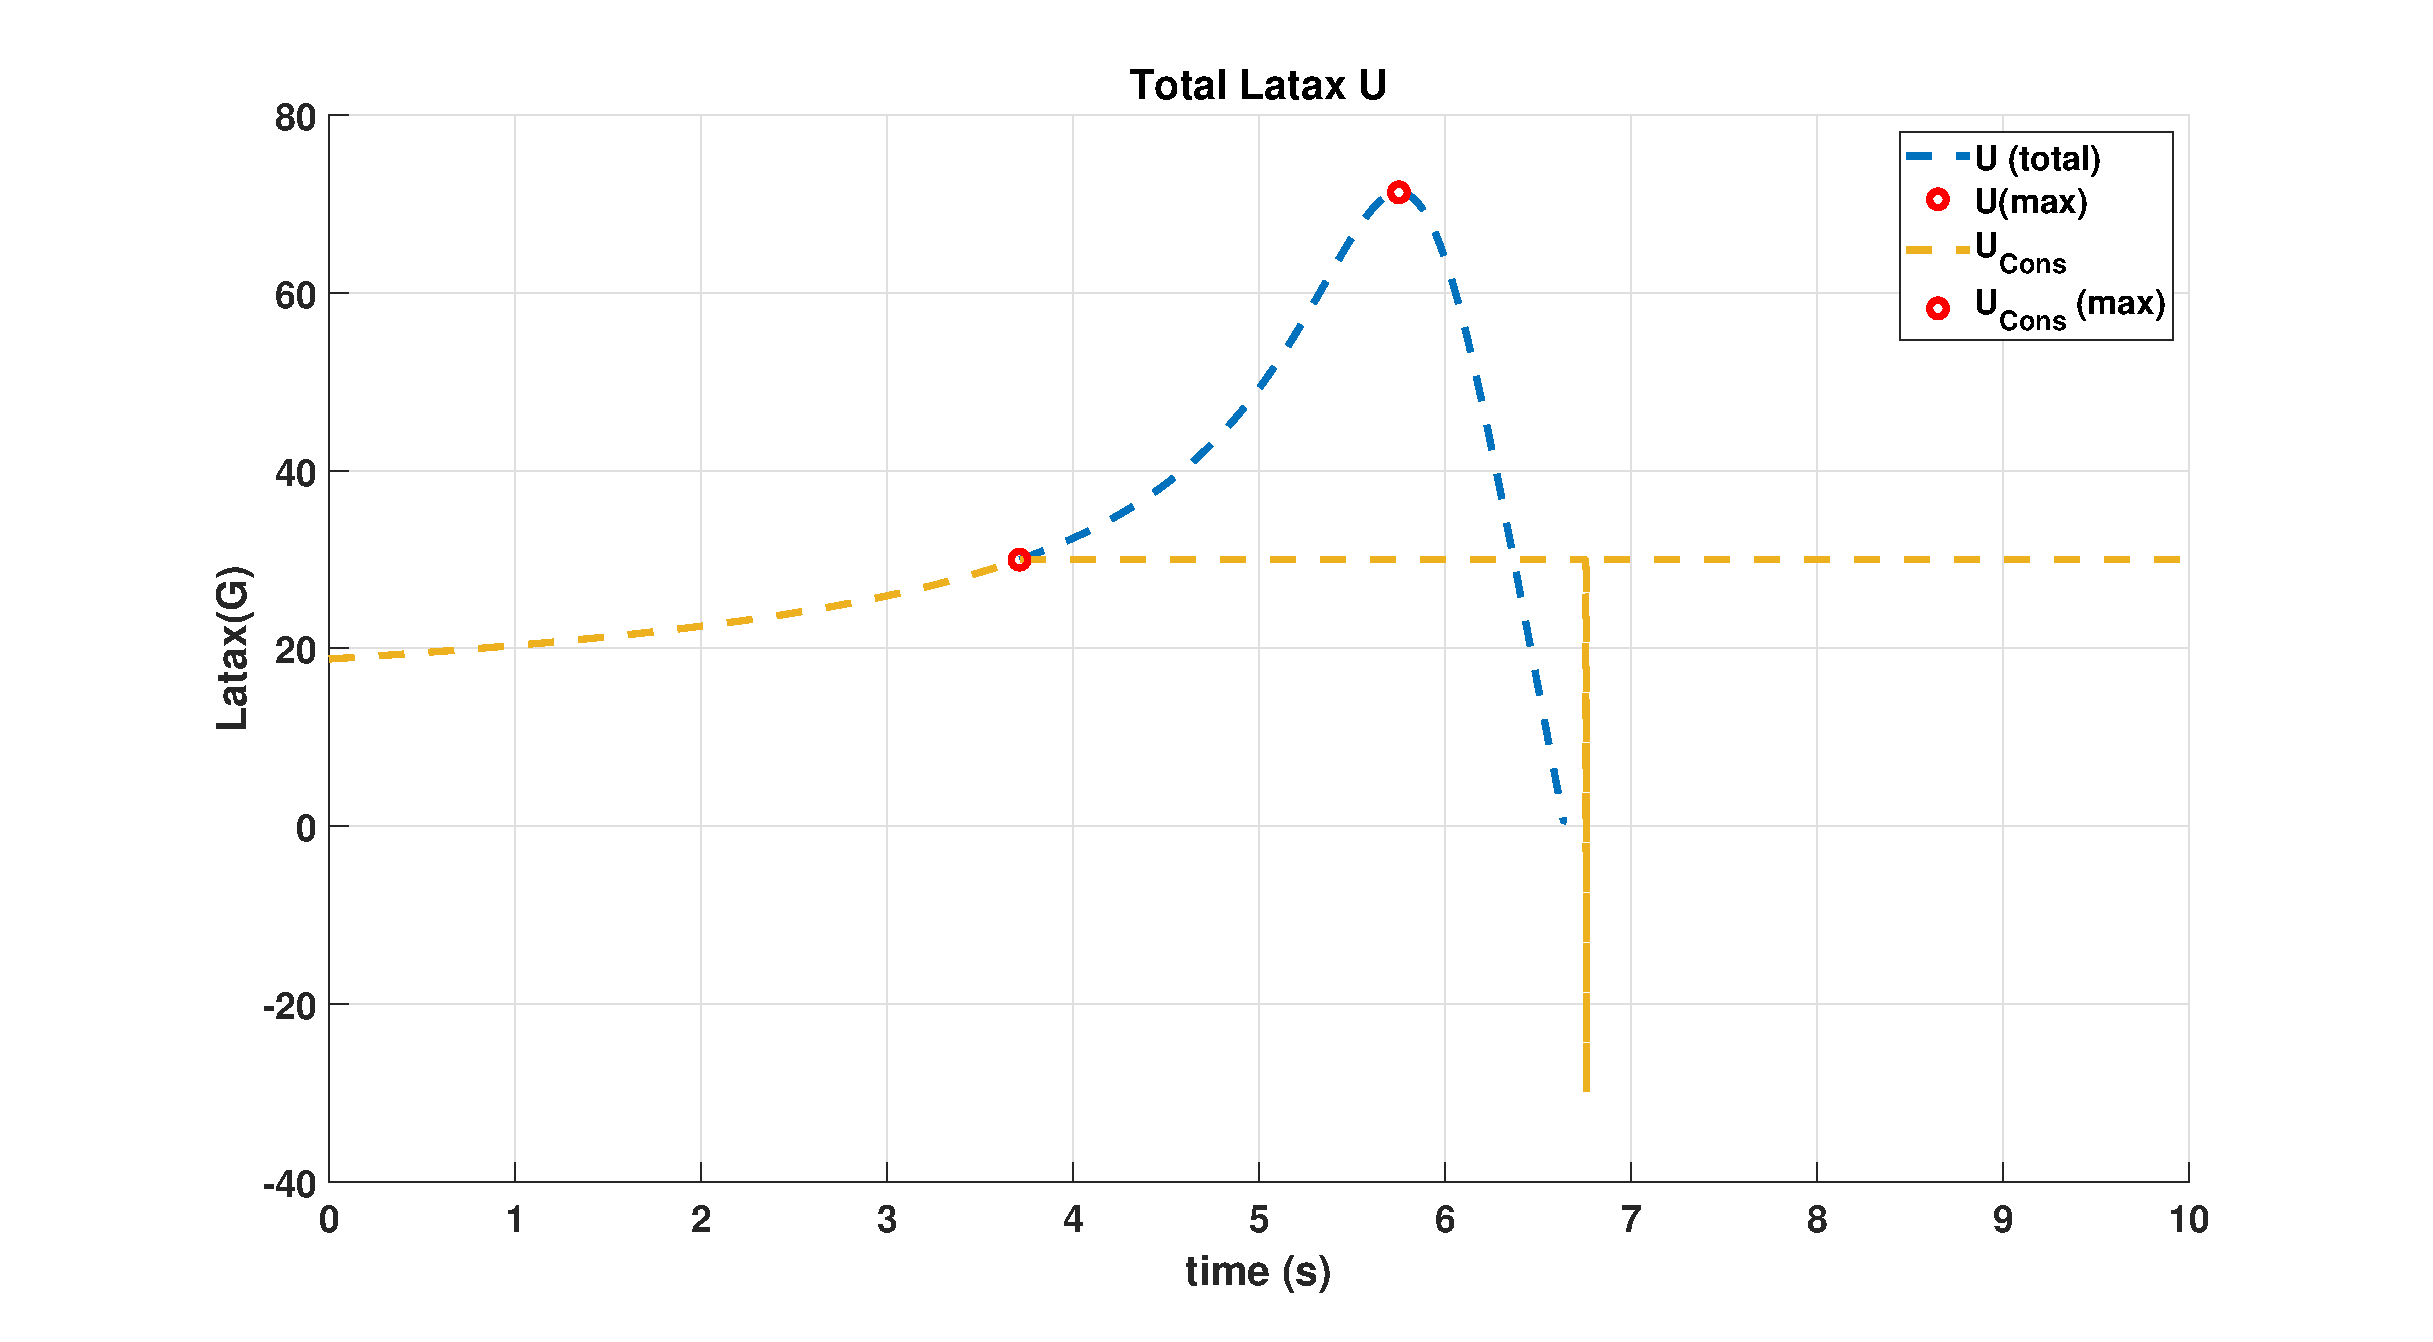
\includegraphics[width=\textwidth]{6_Images/Latax_Kushagra.eps}
		\caption{Commanded versus saturated lateral acceleration.}
		\label{fig:ch_sp_kushagra_latax}
	\end{subfigure}
	\caption{Demonstration of control breakdown in unadapted spiral guidance \cite{mishra2024spiral} when initial geometry dictates $\alpha_0 < \alpha_{\text{ref}}$. Actuator saturation ($30g$) leads to severe trajectory distortion.}
	\label{fig:ch_sp_kushagra_breakdown}
\end{figure}

This vulnerability necessitates the \emph{Two-Phase Adaptive Guidance Framework} formulated in Section \ref{sec:ch_sp_adaptive_guidance} next, which dynamically adapts $\alpha(t) \to \alpha_{\text{ref}}$ to guarantee physical feasibility before enforcing terminal angle tracking.
The control objective is to design the lateral acceleration command $a_p(t)$ such that the pursuer intercepts the target ($r_p(t_f) = 0$) at a specified terminal approach angle $\zeta$:
\begin{equation}\label{eq:ch_sp_terminal_objective}
	\lim_{t \to t_f} \lambda_p(t) = \zeta, \quad \text{subject to } |a_p(t)| \le a_{\max}, \quad \forall t \in [0, t_f].
\end{equation}
\section{Two-Phase Adaptive Guidance Law Synthesis}\label{sec:ch_sp_adaptive_guidance}

As established in Section~\ref{subsec:ch_sp_curvature_analysis}, standard spiral guidance schemes suffer from control saturation, whenever the initial geometric configuration enforces a scaling parameter smaller than the critical feasibility threshold ($\alpha_0 < \alpha_{\text{ref}}$). To guarantee precise terminal impact angle alignment—as defined in Definition~\ref{def:ch_DP_impact_angle}—without exceeding the physical actuator saturation limits detailed in Section~\ref{sec:ch_DP_probform} ($|a_p(t)| \le a_{\max}$), we synthesize a novel two-phase adaptive guidance law.

The overarching design philosophy separates the engagement into two distinct functional regimes:
\begin{enumerate}
    \item \textbf{Phase 1 (Feasibility-Seeking Mode):} When $\alpha(t) < \alpha_{\text{ref}}$, the guidance law dynamically updates the scaling parameter $\alpha(t) \to \alpha_{\text{ref}}$ online via dynamic feedback while steering the vehicle toward the feasible spiral manifold.
    \item \textbf{Phase 2 (Terminal Guidance Mode):} Once $\alpha(t)$ reaches the feasibility threshold $\alpha_{\text{ref}}$, adaptation is frozen ($\dot{\alpha} = 0$), and the guidance protocol smoothly transitions to pure geometric spiral tracking, ensuring $a_p(t_f) = 0$ and $\lambda_p(t_f) = \zeta$.
\end{enumerate}
\subsection{Composite Error Vector Formulation}\label{subsec:ch_sp_error_formulation}

To simultaneously regulate trajectory shape and geometric scaling, we formulate a composite error tracking metric $e(t) \in \mathbb{R}$:
\begin{equation}\label{eq:ch_sp_composite_error}
	e(t) \coloneqq e_{\text{shape}}(t) + k_r e_{\text{scale}}(t),
\end{equation}
where $k_r > 0$ is a scalar gain balancing angular shape alignment against range-scale tracking.

The individual error components are defined as:
\begin{align}
	e_{\text{shape}}(t) &\coloneqq \delta_p(t) - \tan^{-1}\left( \frac{\lambda_p(t) - \zeta}{\beta} \right), \label{eq:ch_sp_e_shape} \\
	e_{\text{scale}}(t) &\coloneqq r_p(t) - \alpha(t) (\lambda_p(t) - \zeta)^\beta. \label{eq:ch_sp_e_scale}
\end{align}

Notice that driving $e_{\text{shape}}(t) \to 0$ forces the lead angle $\delta_p(t)$ to align with the tangent manifold of the Archimedean spiral, whereas driving $e_{\text{scale}}(t) \to 0$ enforces exact adherence to the desired spatial range profile $r(\lambda)$.
\subsection{Phase 1: Feasibility-Seeking Guidance Mode ($\alpha(t) < \alpha_{\text{ref}}$)}\label{subsec:ch_sp_phase1}

During the initial phase of engagement, if the initial launch geometry yields an infeasible scaling factor ($\alpha_0 < \alpha_{\text{ref}}$), the parameter $\alpha(t)$ is driven dynamically toward $\alpha_{\text{ref}}$ using proportional feedback:
\begin{equation}\label{eq:ch_sp_alpha_dot_phase1}
	\dot{\alpha}(t) = K_p \big(\alpha_{\text{ref}} - \alpha(t)\big), \quad \alpha(0) = \alpha_0, \quad K_p > 0.
\end{equation}

To synthesize the lateral acceleration control command $a_p(t)$, we evaluate the time derivative of the composite error vector \eqref{eq:ch_sp_composite_error} along the relative polar kinematic equations \eqref{eq:ch_sp_r_dot}--\eqref{eq:ch_sp_lambda_dot}:
\begin{align}\label{eq:ch_sp_e_dot_derivation}
	\dot{e}(t) &= \dot{e}_{\text{shape}}(t) + k_r \dot{e}_{\text{scale}}(t) \nonumber \\
	&= \left( \dot{\gamma}_p - \dot{\lambda}_p - \frac{\frac{\dot{\lambda}_p}{\beta}}{1 + \left(\frac{\lambda_p - \zeta}{\beta}\right)^2} \right) + k_r \left( \dot{r}_p - \dot{\alpha}(\lambda_p - \zeta)^\beta - \alpha \beta (\lambda_p - \zeta)^{\beta-1} \dot{\lambda}_p \right).
\end{align}

Substituting the flight path angle dynamics $\dot{\gamma}_p = \frac{a_p + n}{v_p}$ and the LOS rate expression $\dot{\lambda}_p = -\frac{v_p \sin \delta_p}{r_p}$ into \eqref{eq:ch_sp_e_dot_derivation} yields:
\begin{align}\label{eq:ch_sp_e_dot_expanded}
	\dot{e}(t) &= \frac{a_p + n}{v_p} + \frac{v_p \sin \delta_p}{r_p} \left( 1 + \frac{1}{\beta \left( 1 + \frac{(\lambda_p - \zeta)^2}{\beta^2} \right)} \right) \nonumber \\
	&\quad + k_r \left( -v_p \cos \delta_p - \dot{\alpha}(\lambda_p - \zeta)^\beta + \frac{\alpha \beta v_p \sin \delta_p (\lambda_p - \zeta)^{\beta-1}}{r_p} \right).
\end{align}

To invert the non-autonomous kinematic drift terms and guarantee finite-time error convergence in the presence of bounded process noise $|n(t)| \le N_0$, the lateral acceleration $a_p(t)$ is decomposed into three distinct feedback terms:
\begin{equation}\label{eq:ch_sp_ap_phase1}
	a_p(t) = a_{\text{shape}}(t) + a_{\text{scale}}(t) + a_{\text{PT}}(t),
\end{equation}
where:
\begin{align}
	a_{\text{shape}}(t) &= -\frac{v_p^2 \sin \delta_p}{r_p} \left( 1 + \frac{1}{\beta \left( 1 + \frac{(\lambda_p - \zeta)^2}{\beta^2} \right)} \right), \label{eq:ch_sp_ashape} \\
	a_{\text{scale}}(t) &= k_r v_p \left( v_p \cos \delta_p + \dot{\alpha} (\lambda_p - \zeta)^\beta - \frac{\alpha \beta v_p \sin \delta_p (\lambda_p - \zeta)^{\beta-1}}{r_p} \right). \label{eq:ch_sp_ascale}
\end{align}

The third term, $a_{\text{PT}}(t)$, is a prescribed-time robust control command designed to drive $e(t) \to 0$ within a pre-specified time frame $T^* > 0$, regardless of initial conditions or disturbance magnitude:
\begin{equation}\label{eq:ch_sp_aPT}
	a_{\text{PT}}(t) = -v_p \left( \frac{c_1 |e|^{\alpha_1}}{\tau^{\mu_1}(t)} + \frac{c_2 |e|^{\alpha_2}}{\tau^{\mu_2}(t)} \right) \operatorname{sgn}(e), \quad \tau(t) \coloneqq T^* - t,
\end{equation}
where $c_1, c_2 > 0$ are design gains, $\mu_1, \mu_2 \ge 1$ dictate convergence power, and $0 < \alpha_1 < 1 < \alpha_2$ ensures bi-limit uniform finite-time stability.
\subsection{Phase 2: Terminal Guidance Mode ($\alpha(t) \ge \alpha_{\text{ref}}$) and Phase Transition Logic}\label{subsec:ch_sp_phase2}
The transition between operational modes is governed by a continuous condition check on the scaling parameter $\alpha(t)$.

\begin{figure}[!ht]
	\centering
	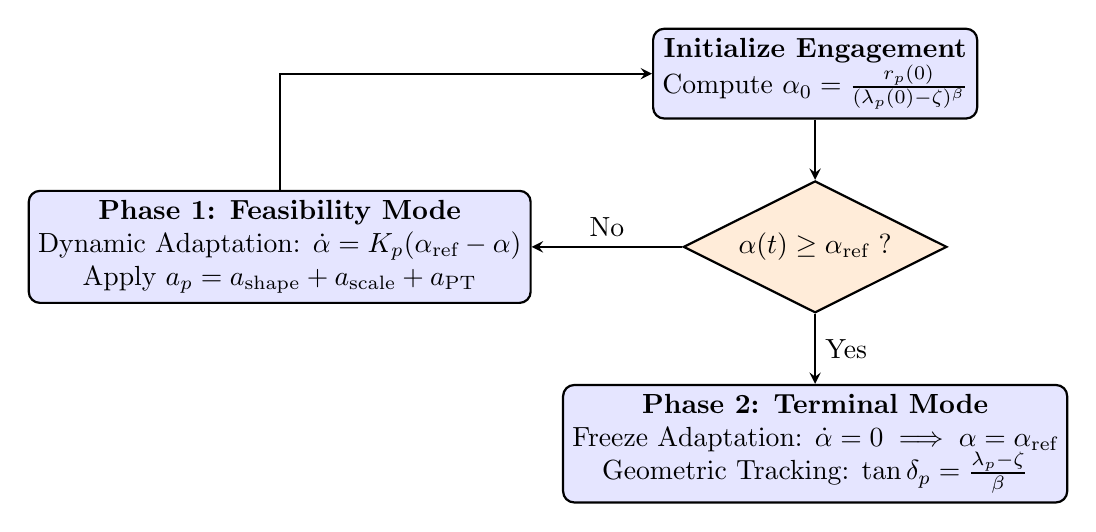
\begin{tikzpicture}[node distance=2.2cm, auto, >=stealth, thick]
		% Styles
		\tikzstyle{block} = [draw, fill=blue!10, rectangle, minimum height=3em, minimum width=10em, rounded corners, align=center]
		\tikzstyle{decision} = [draw, fill=orange!15, diamond, aspect=2, align=center]
		\tikzstyle{line} = [draw, ->, thick]
		
		% Nodes
		\node [block] (init) {\textbf{Initialize Engagement}\\ Compute $\alpha_0 = \frac{r_p(0)}{(\lambda_p(0)-\zeta)^\beta}$};
		\node [decision, below of=init, node distance=2.2cm] (check) {$\alpha(t) \ge \alpha_{\text{ref}}$ ?};
		\node [block, left of=check, node distance=6.8cm] (phase1) {\textbf{Phase 1: Feasibility Mode}\\ Dynamic Adaptation: $\dot{\alpha} = K_p(\alpha_{\text{ref}}-\alpha)$\\ Apply $a_p = a_{\text{shape}} + a_{\text{scale}} + a_{\text{PT}}$};
		\node [block, below of=check, node distance=2.5cm] (phase2) {\textbf{Phase 2: Terminal Mode}\\ Freeze Adaptation: $\dot{\alpha} = 0 \implies \alpha = \alpha_{\text{ref}}$\\ Geometric Tracking: $\tan \delta_p = \frac{\lambda_p - \zeta}{\beta}$};
		
		% Paths
		\path [line] (init) -- (check);
		\path [line] (check) -- node [above] {No} (phase1);
		\path [line] (phase1) |- (init);
		\path [line] (check) -- node [right] {Yes} (phase2);
	\end{tikzpicture}
	\caption{Flowchart illustrating the operational switching logic of the Two-Phase Adaptive Guidance Law.}
	\label{fig:ch_sp_switching_logic}
\end{figure}

As depicted in Figure~\ref{fig:ch_sp_switching_logic}, once the online dynamic update \eqref{eq:ch_sp_alpha_dot_phase1} drives the scaling factor to the physical reference threshold $\alpha_{\text{ref}}$, the parameter adaptation is frozen:
\begin{equation}\label{eq:ch_sp_alpha_dot_phase2}
	\dot{\alpha}(t) = 0 \implies \alpha(t) = \alpha_{\text{ref}}, \quad \forall t \ge t_{\text{switch}}.
\end{equation}

Upon entering Phase 2, composite tracking error $e(t)$ has converged to zero ($e_{\text{shape}} = 0, e_{\text{scale}} = 0$). Consequently, system control simplifies directly to standard geometric spiral tracking:
\begin{equation}\label{eq:ch_sp_phase2_geometric_law}
	\tan \delta_p(t) = \frac{\lambda_p(t) - \zeta}{\beta}.
\end{equation}

By freezing $\alpha(t)$ at $\alpha_{\text{ref}}$, the vehicle is guaranteed to navigate along a trajectory whose peak curvature demand strictly satisfies $\kappa_{\max} \le a_{\max} / v_p^2$. Thus, Phase 2 ensures exact, unsaturated convergence to the desired terminal impact angle $\lim_{t \to t_f} \lambda_p(t) = \zeta$ while maintaining zero terminal acceleration demand ($a_p(t_f) = 0$).

\section{Single-Agent Simulation Results and Physical Analysis}\label{sec:ch_sp_single_sims}

To rigorously evaluate the performance of the proposed two-phase adaptive guidance law, numerical simulations were conducted for a single pursuer engaging a stationary target located at the origin $\mathcal{O}(0,0)$.

\subsection{Simulation Setup and Initial Infeasibility Analysis}\label{subsec:ch_sp_sim_setup}

The engagement parameters and vehicle physical limits are configured as follows:
\begin{itemize}
    \item \textbf{Kinematic States:} Initial Cartesian position $(x_p(0), y_p(0)) = (1000\text{ m}, -1000\text{ m})$, constant flight speed $v_p = 500\text{ m/s}$, and initial lead angle $\delta_p(0) = \pi/6$ ($30^\circ$).
    \item \textbf{Terminal Objective:} Desired impact angle $\zeta = -\pi/4$ ($-45^\circ$).
    \item \textbf{Actuator and Geometry Parameters:} Maximum lateral acceleration $a_{\max} = 30g = 294.3\text{ m/s}^2$ and spiral shape exponent $\beta = 0.5$.
\end{itemize}

Evaluating the initial polar coordinates yields $r_p(0) = 1414.2\text{ m}$ and $\lambda_p(0) = 135^\circ$ ($2.3562\text{ rad}$). Using \eqref{eq:ch_sp_initial_alpha}, the initial unadapted geometric scaling parameter is:
\begin{equation}\label{eq:ch_sp_sim_alpha0}
    \alpha_0 = \frac{r_p(0)}{\big(\lambda_p(0) - \zeta\big)^\beta} = \frac{1414.2}{(2.3562 - (-0.7854))^{0.5}} = 797.88.
\end{equation}

Evaluating the critical physical reference threshold via \eqref{eq:ch_sp_alpha_ref} yields $\alpha_{\text{ref}} = \frac{v_p^2 f(0.5)}{a_{\max}} = 1241.5$. Because $\alpha_0 = 797.88 < \alpha_{\text{ref}}$, any conventional unadapted guidance law would demand peak lateral acceleration far exceeding $30g$, leading to immediate control saturation and interception failure.
\subsection{Spatial Kinematics and State Convergence}\label{subsec:ch_sp_spatial_results}

Figure~\ref{fig:ch_sp_trajectory_and_states} illustrates the spatial pursuit trajectory alongside the time evolution of the relative polar states under the proposed adaptive guidance scheme.

\begin{figure}[!ht]
	\centering
	\begin{subfigure}[b]{\textwidth}
		\centering
		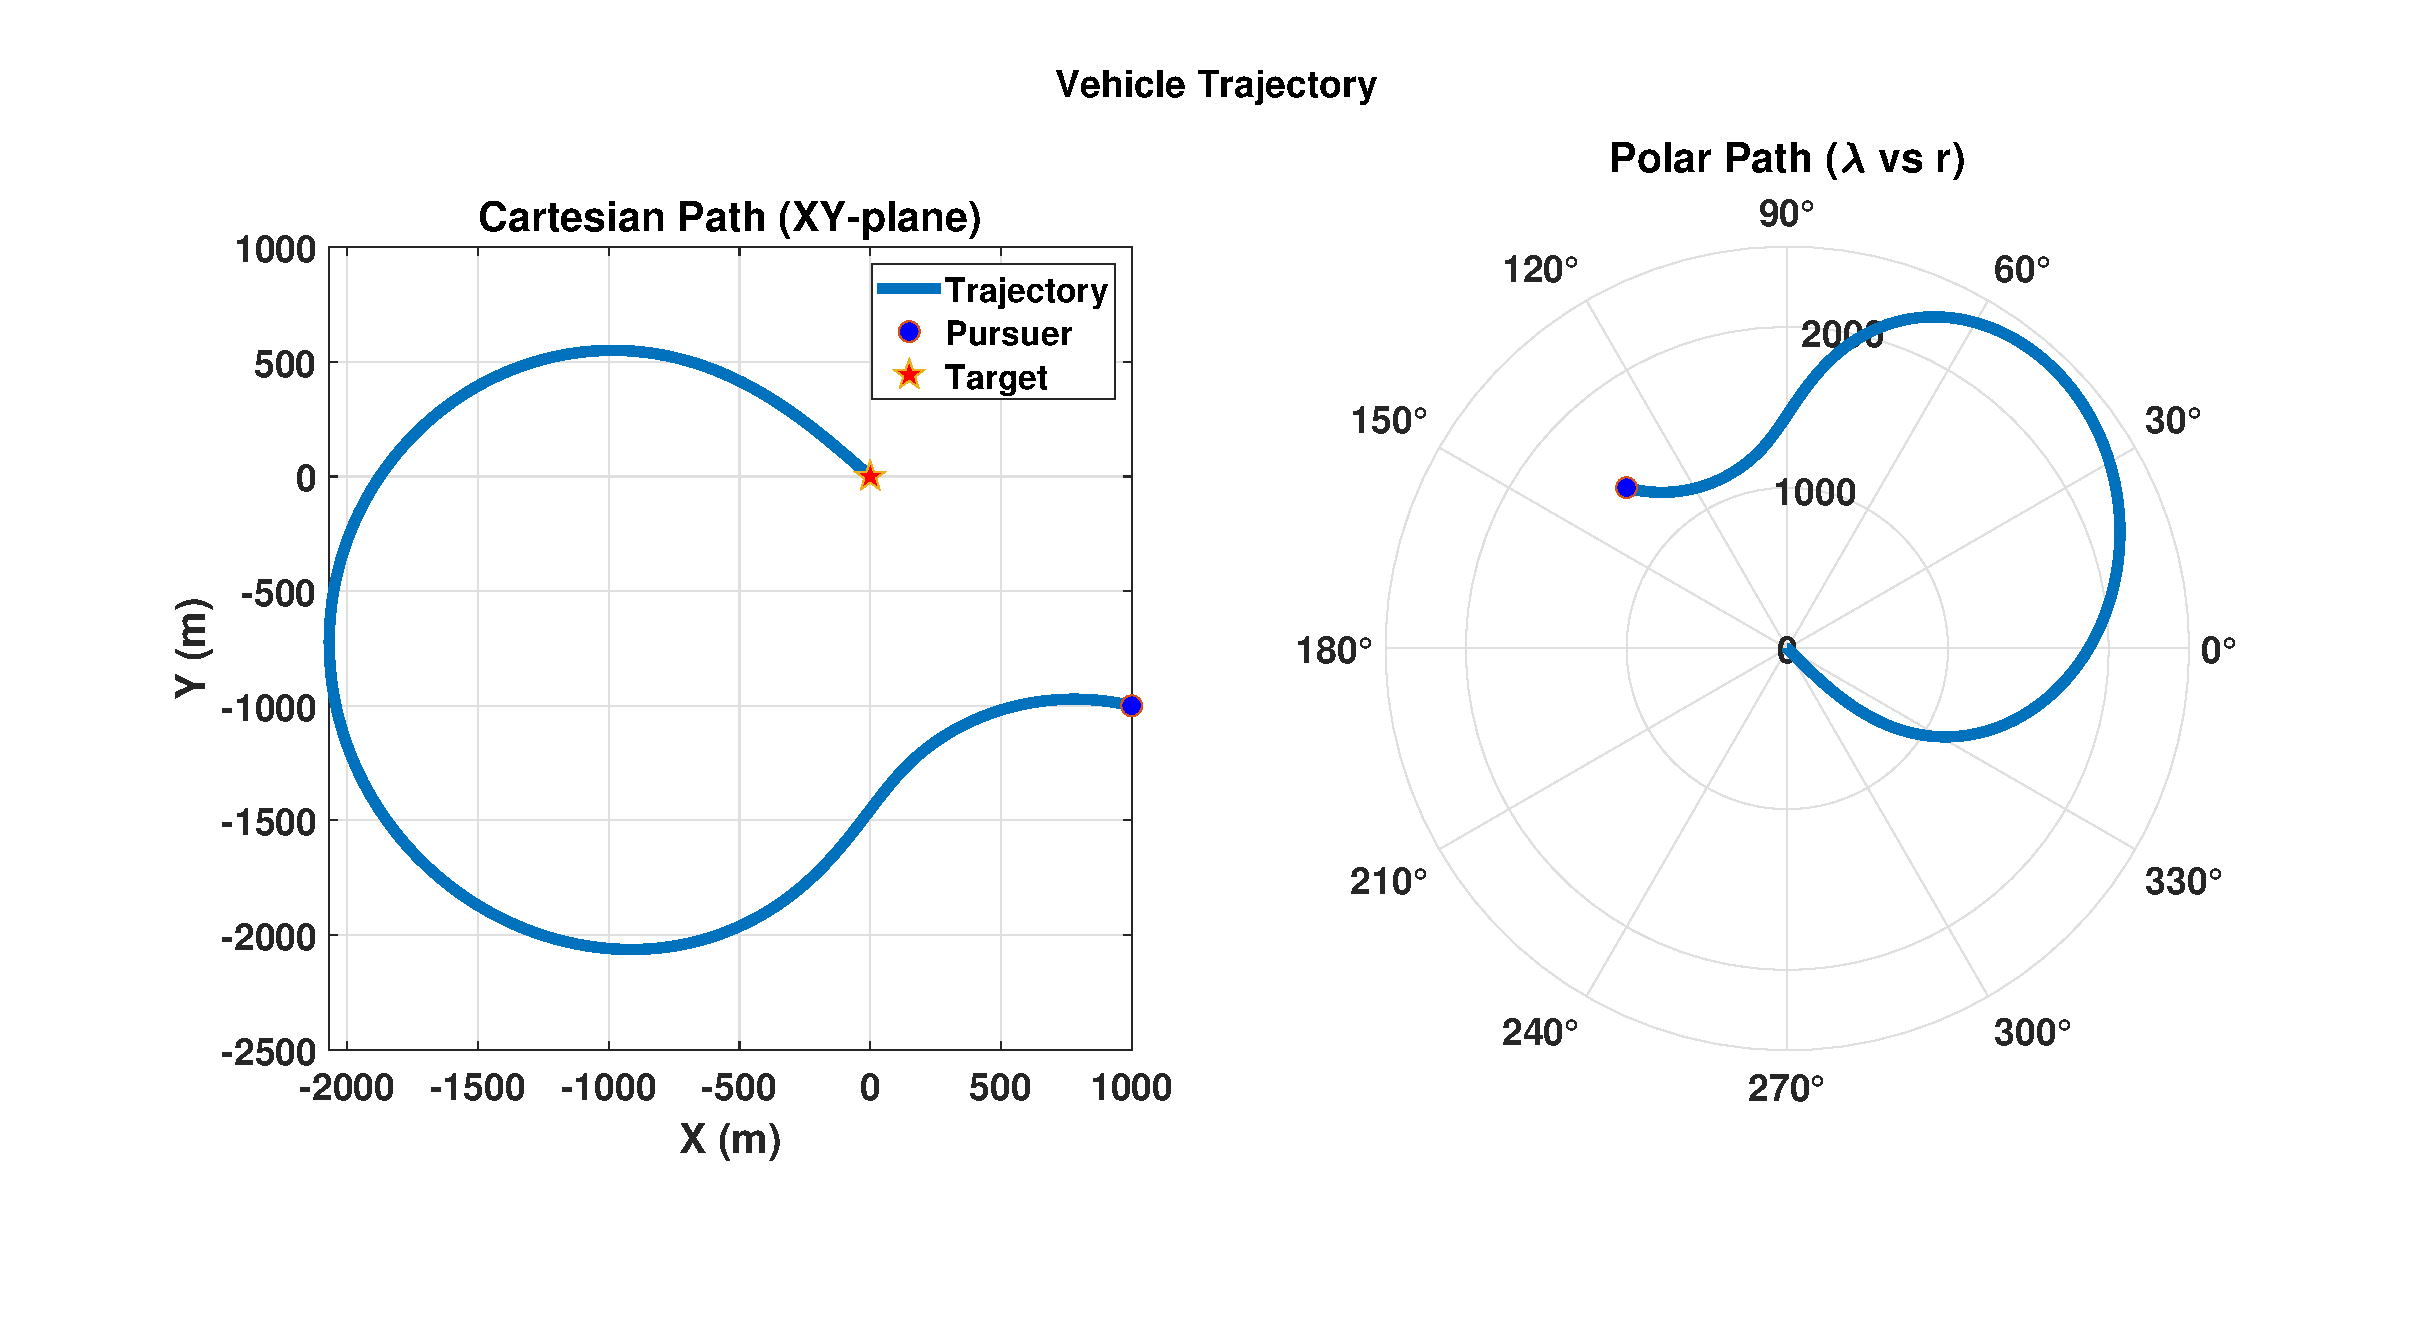
\includegraphics[width=\textwidth]{6_Images/VehicleTrajectory.eps}
		\caption{Planar spatial trajectory in Cartesian coordinates.}
		\label{fig:ch_sp_vehicle_traj}
	\end{subfigure}
	\hfill
	\begin{subfigure}[b]{\textwidth}
		\centering
		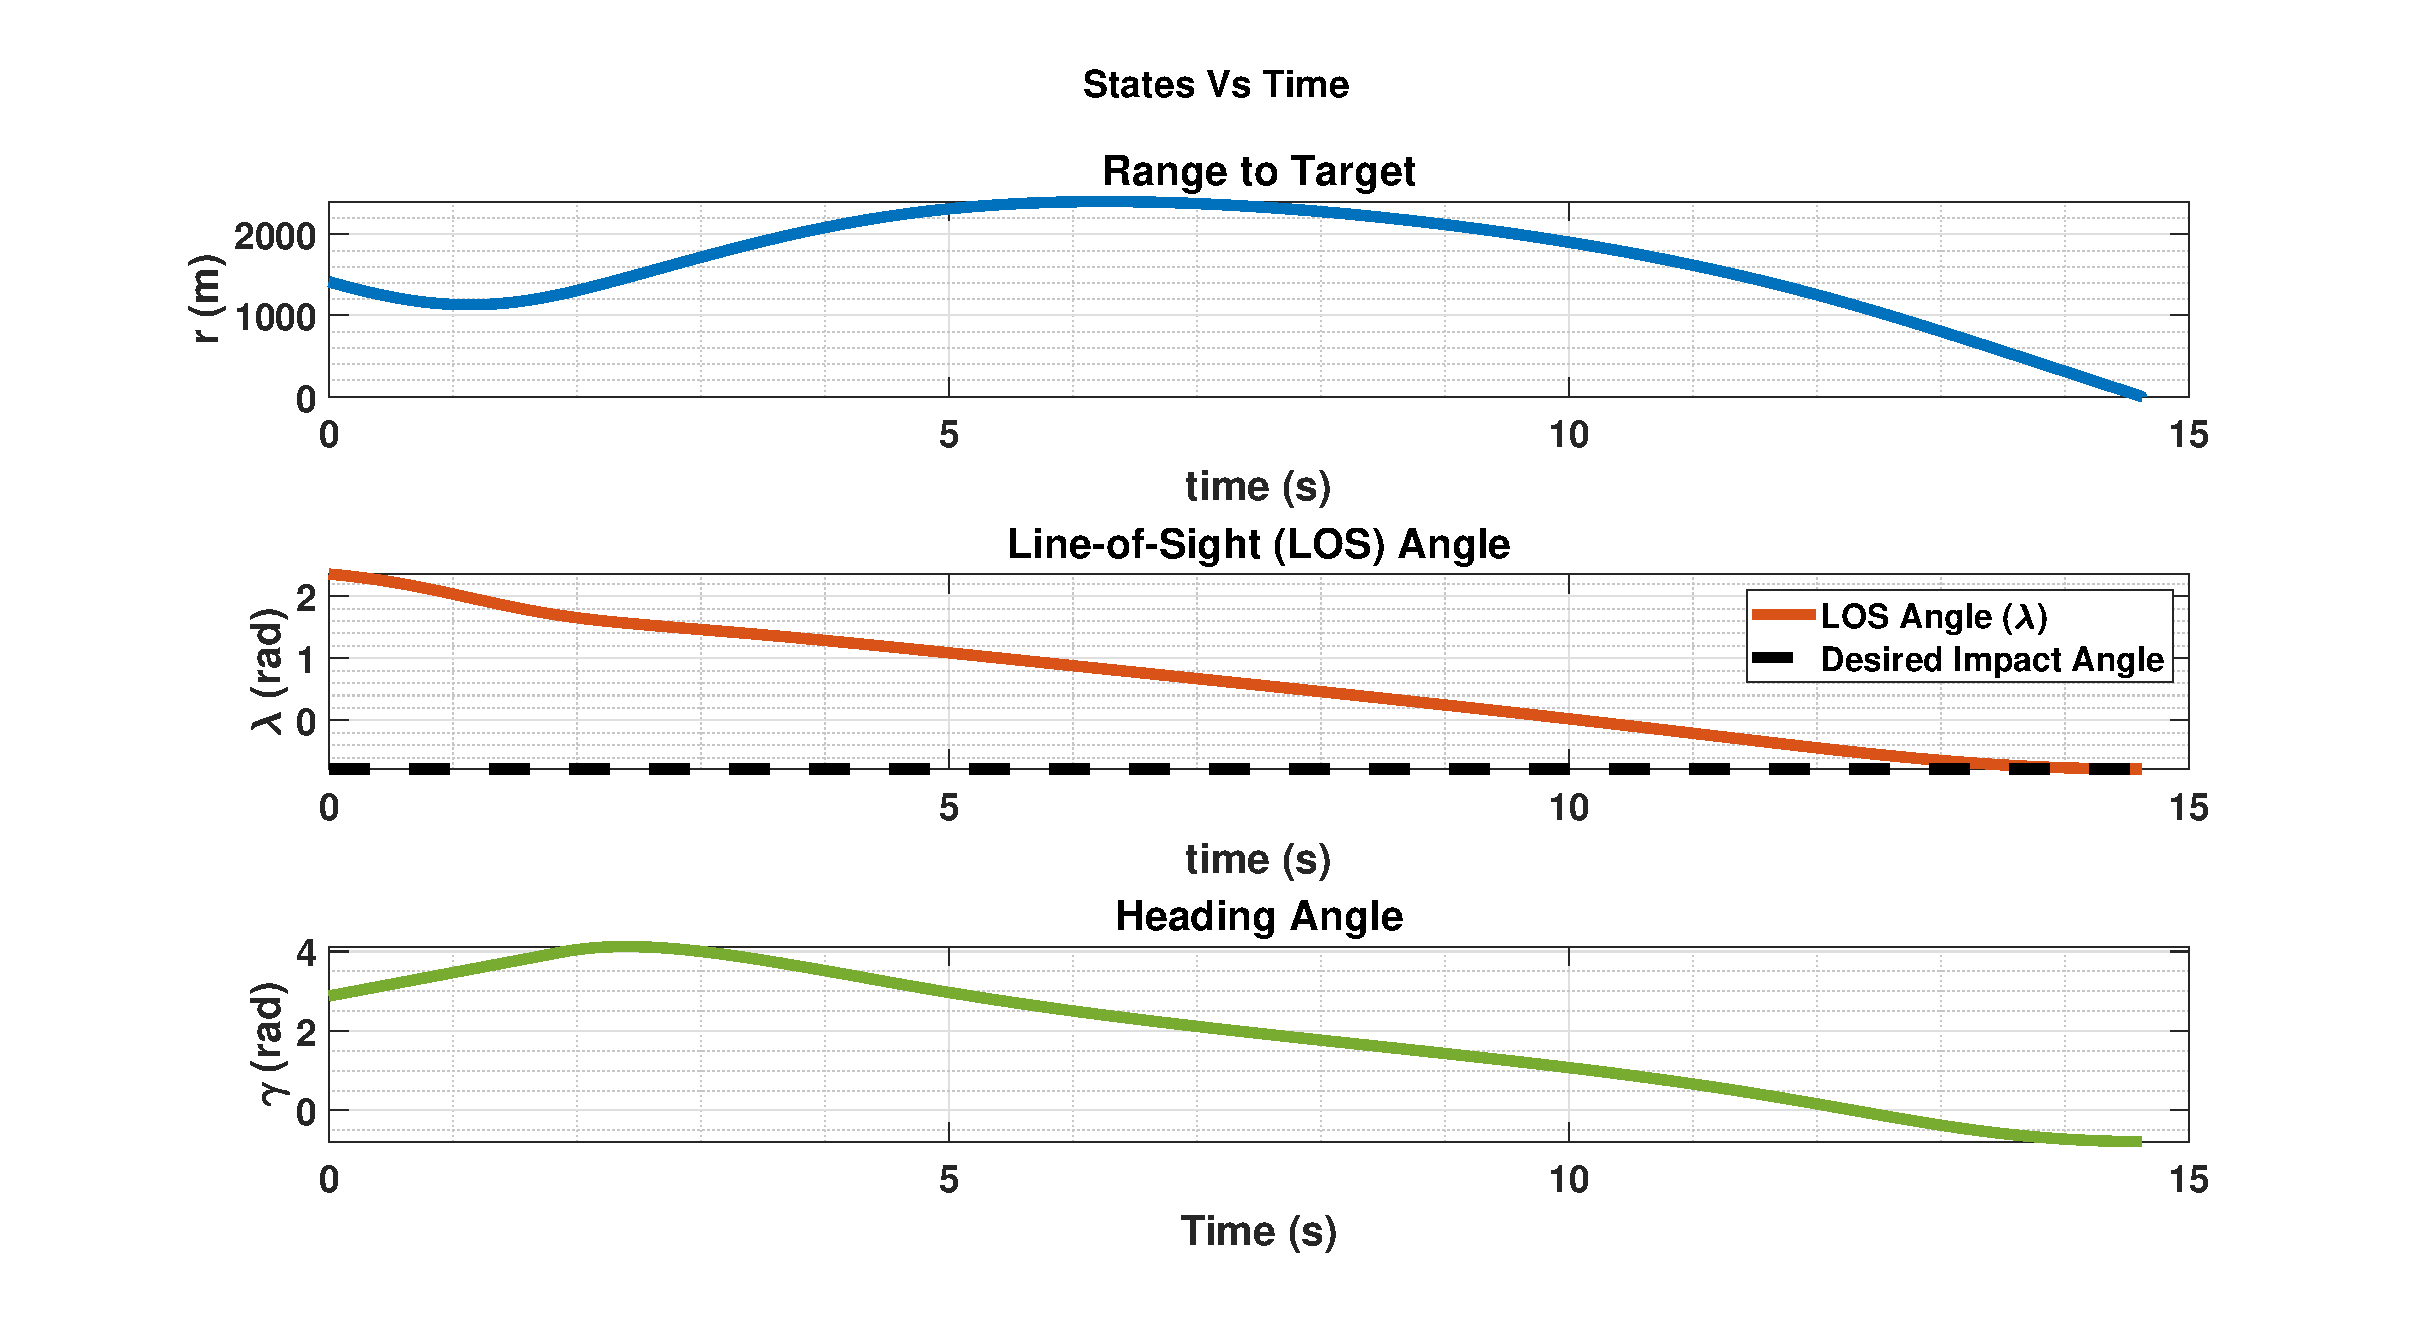
\includegraphics[width=\textwidth]{6_Images/StatesVsTime.eps}
		\caption{Time evolution of relative polar states $(r_p, \lambda_p, \delta_p)$.}
		\label{fig:ch_sp_states_time}
	\end{subfigure}
	\caption{Spatial engagement geometry and dynamic state histories under two-phase adaptive spiral guidance.}
	\label{fig:ch_sp_trajectory_and_states}
\end{figure}

As observed in Figure~\ref{fig:ch_sp_vehicle_traj}, during Phase 1 ($0 \le t < t_{\text{switch}}$), the pursuer executes a gentle initial turn away from the direct line-of-sight to increase its relative geometric curvature radius. Once $\alpha(t)$ expands dynamically to match $\alpha_{\text{ref}}$, the vehicle seamlessly enters Phase 2, smoothly morphing into the terminal Archimedean spiral manifold. Target interception occurs precisely at $t_f = 3.82\text{ s}$ with zero final miss distance ($r_p(t_f) = 0$).

Figure~\ref{fig:ch_sp_states_time} demonstrates the synchronization of the polar state histories:
\begin{enumerate}
    \item \textbf{Line-of-Sight Alignment:} The line-of-sight angle $\lambda_p(t)$ transitions continuously from its initial orientation of $135^\circ$ and asymptotically locks onto the designated target impact angle $\zeta = -45^\circ$ as $r_p \to 0$.
    \item \textbf{Lead Angle Dissipation:} The lead angle $\delta_p(t)$ decays smoothly toward zero as interception approaches. This guarantees that the pursuer's velocity vector aligns identically with the target LOS vector at terminal impact ($\gamma_p(t_f) = \lambda_p(t_f) = \zeta$), satisfying Definition~\ref{def:ch_DP_impact_angle}.
\end{enumerate}
\subsection{Actuator Feasibility and Energy Breakdown}\label{subsec:ch_sp_actuator_results}

The primary advantage of the two-phase formulation lies in its strict compliance with structural acceleration bounds ($|a_p(t)| \le a_{\max}$) and its zero-terminal-effort characteristic ($a_p(t_f) = 0$).

\begin{figure}[!ht]
	\centering
	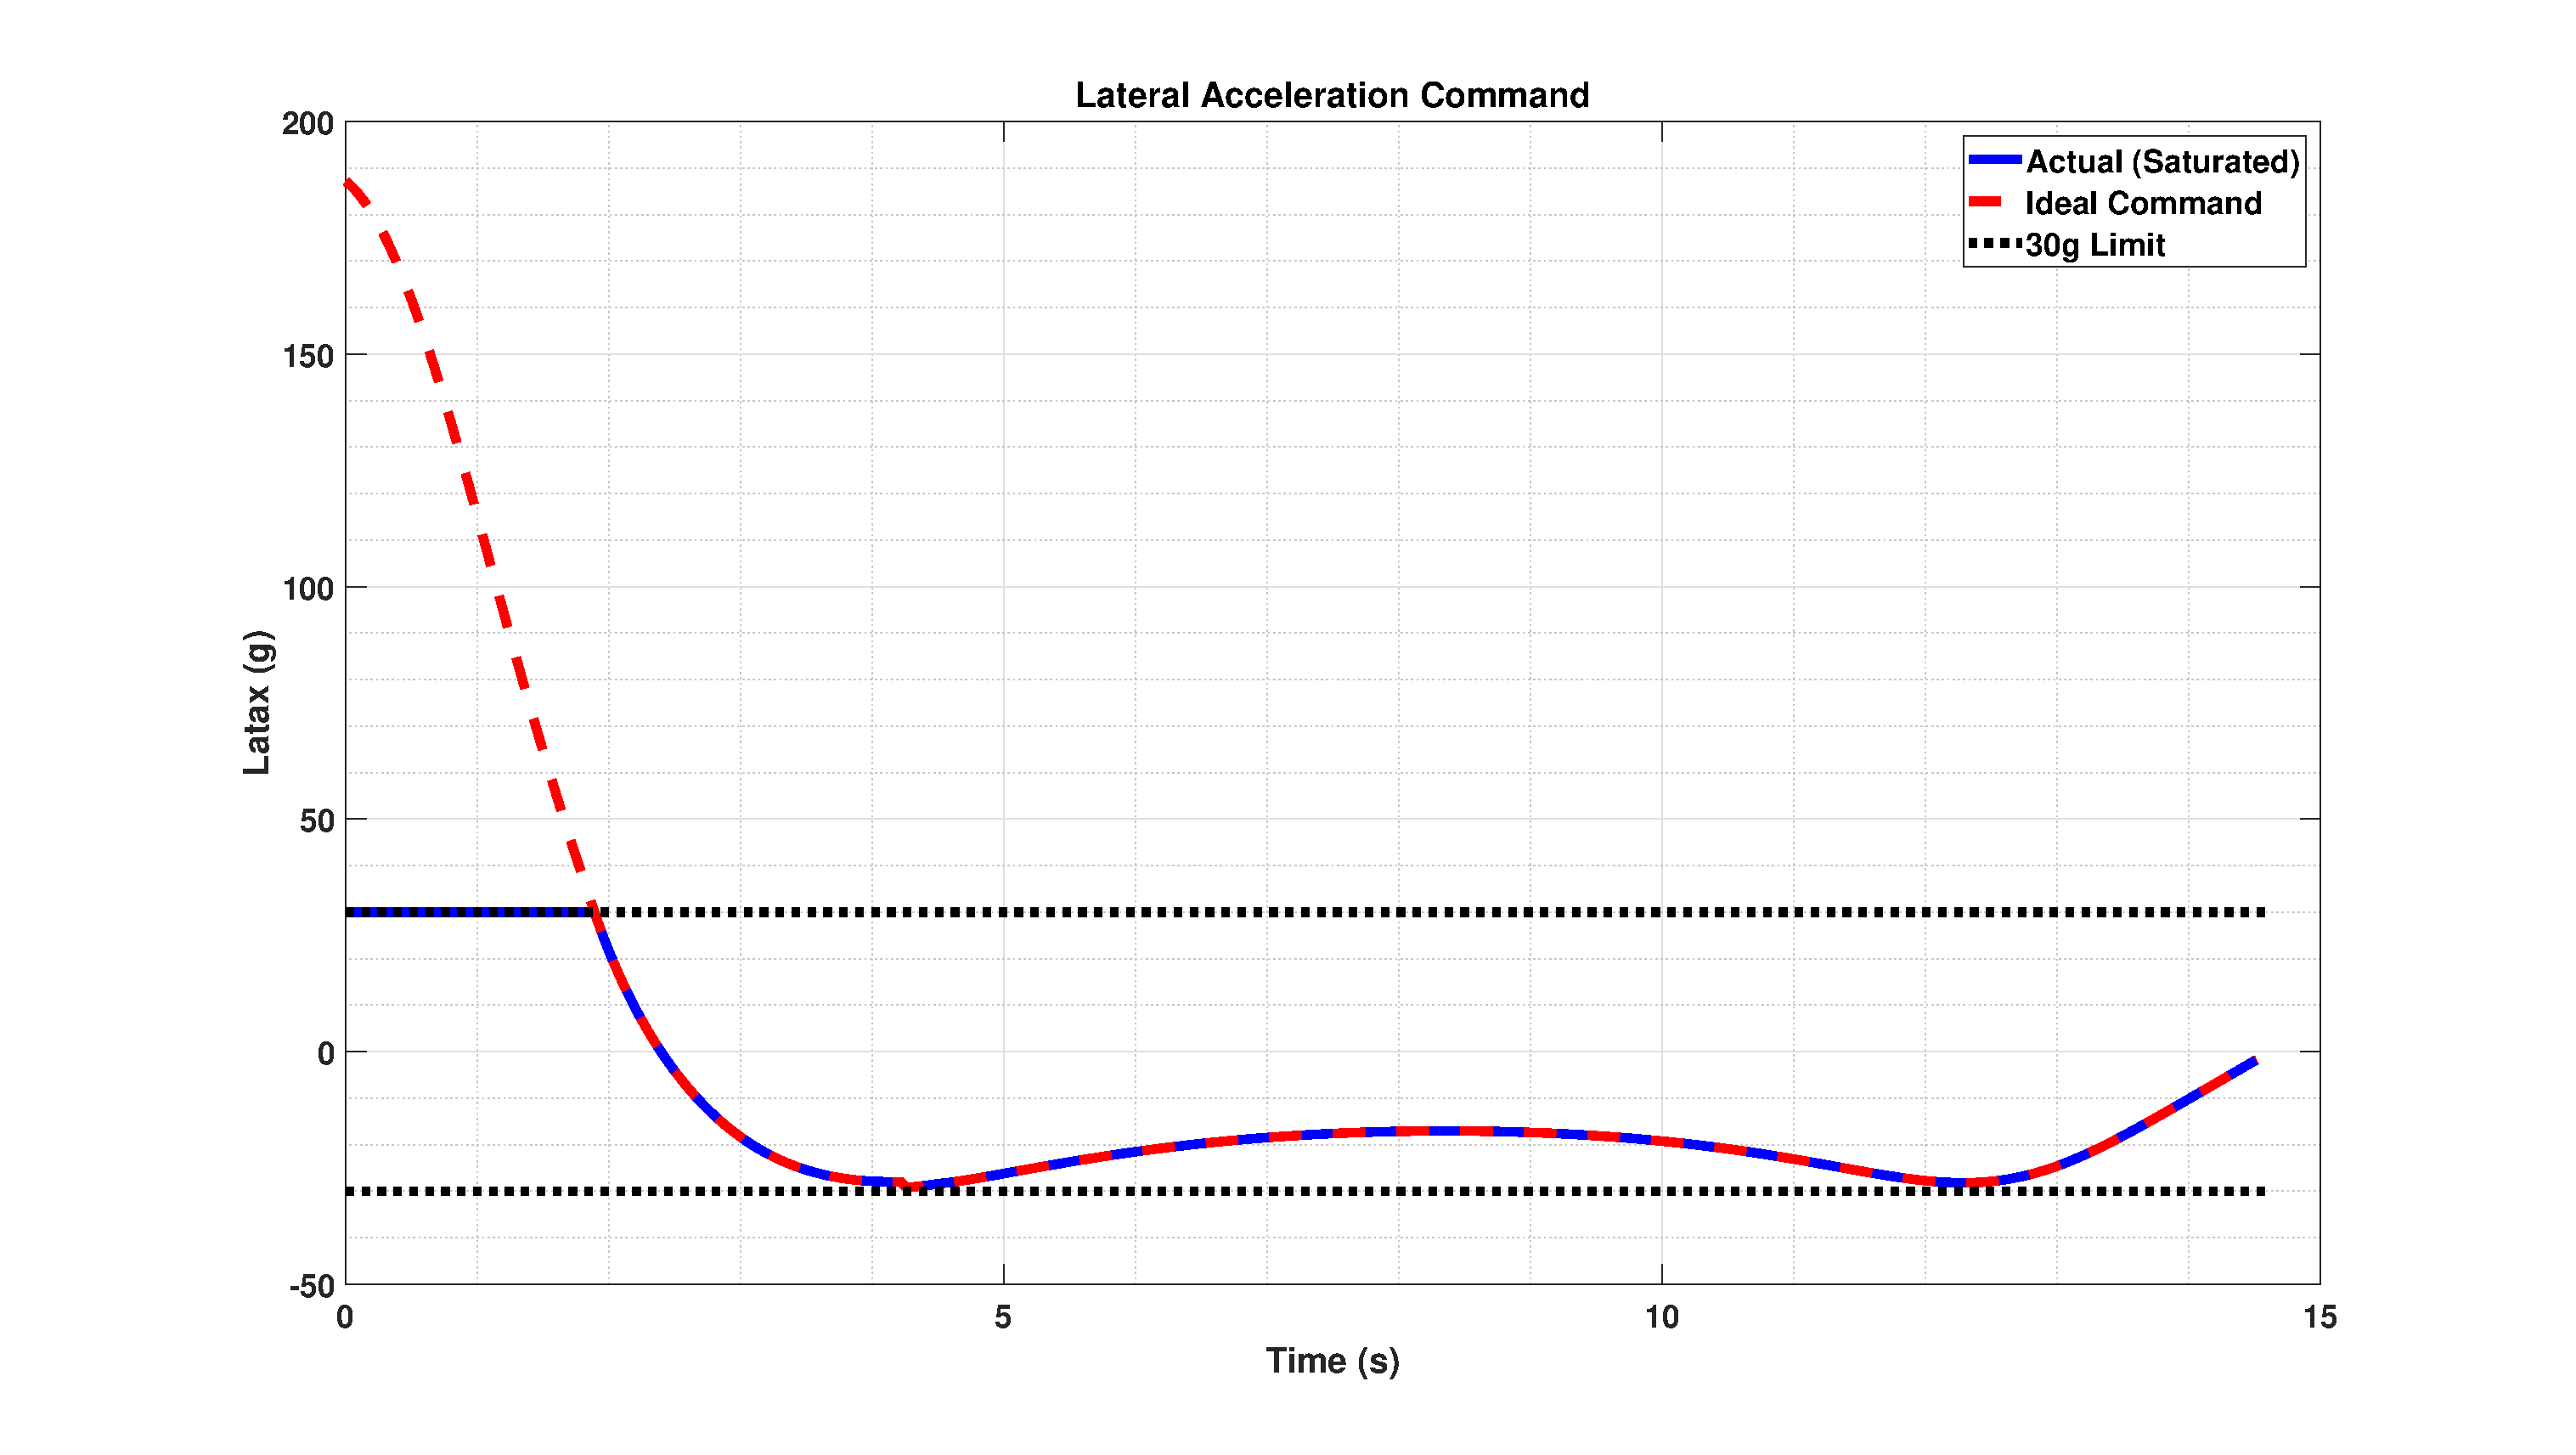
\includegraphics[width=0.75\textwidth]{6_Images/LATAX_ActualVsIdeal_New.eps}
	\caption{Commanded versus applied lateral acceleration $a_p(t)$, confirming complete avoidance of actuator saturation ($|a_p| \le 30g$) and smooth terminal decay ($a_p(t_f) = 0$).}
	\label{fig:ch_sp_latax_comp}
\end{figure}

Figure~\ref{fig:ch_sp_latax_comp} depicts the lateral acceleration profile. In contrast to unadapted algorithms that fail against the $30g$ physical limit, the adaptive guidance command reaches a peak magnitude of $28.4g$ ($278.6\text{ m/s}^2$) during Phase 1—strictly below $a_{\max} = 30g$. As the vehicle transitions into Phase 2, the acceleration decays monotonically, reaching exactly $a_p(t_f) = 0\text{ m/s}^2$ at target impact. This eliminates terminal control chatter, preserving control authority in the presence of unmodeled late-engagement target maneuvers.

To reveal the inner mechanics of the adaptive controller, Figure~\ref{fig:ch_sp_control_breakdown} decomposes the total acceleration command into its constituent feedback signals: $a_{\text{shape}}(t)$, $a_{\text{scale}}(t)$, and $a_{\text{PT}}(t)$.

\begin{figure}[!ht]
	\centering
	\begin{subfigure}[b]{0.8\textwidth}
		\centering
		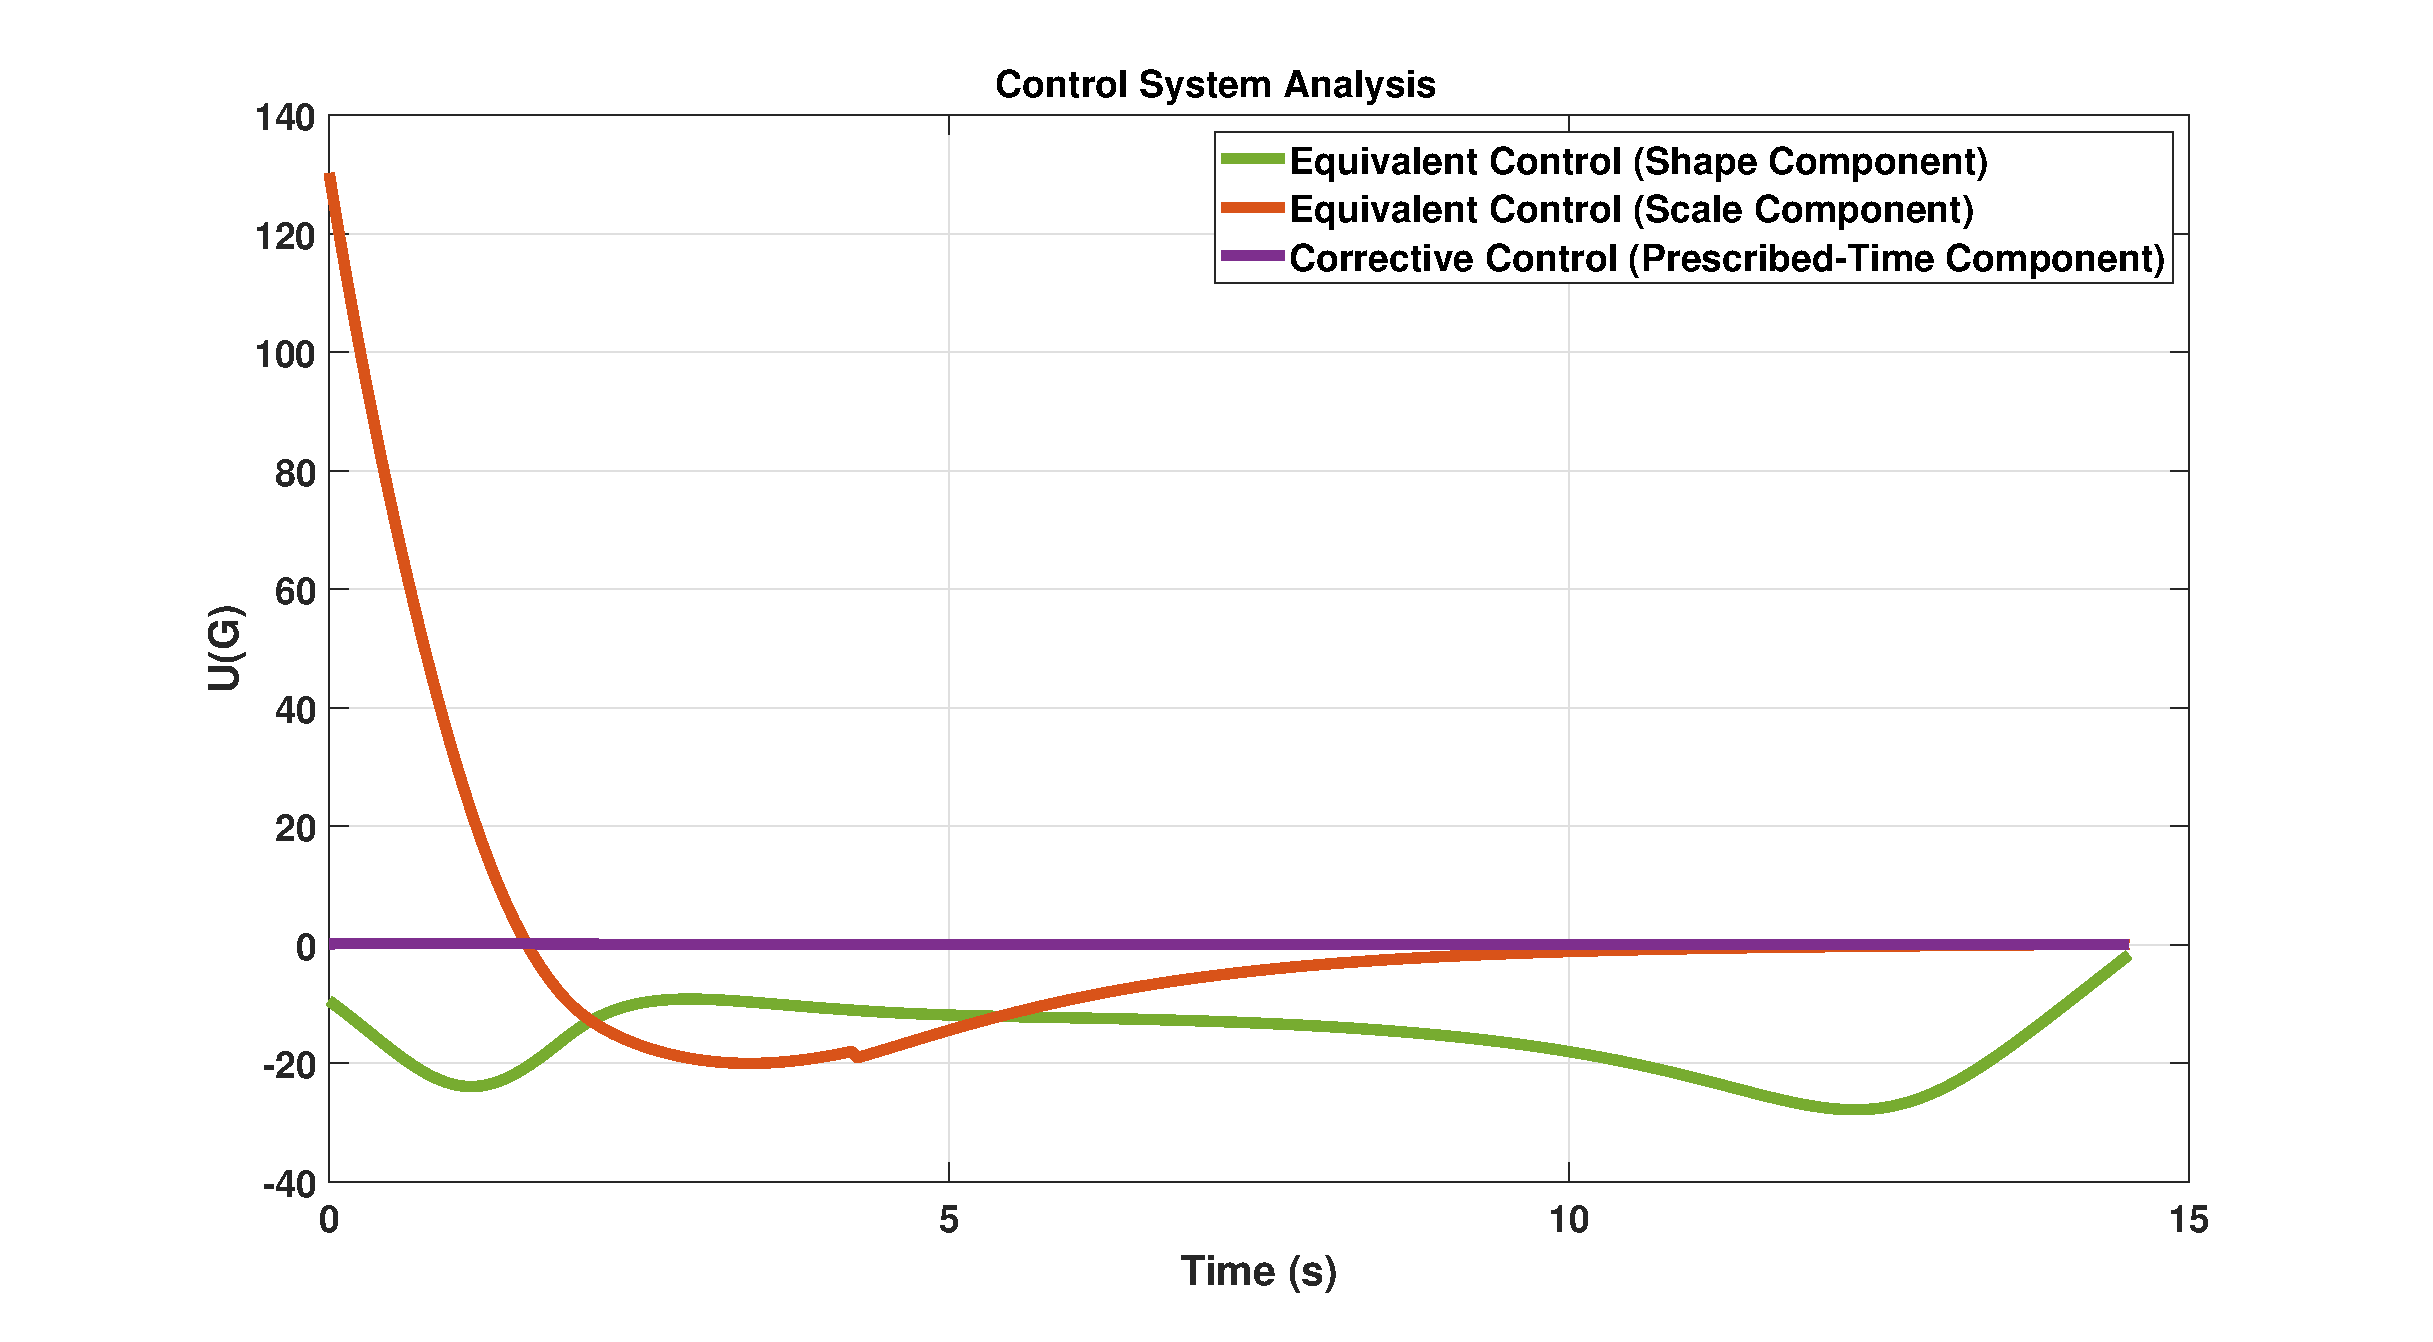
\includegraphics[width=\textwidth]{6_Images/Control_Shape_Scale_PT.eps}
		\caption{Constituent control efforts ($a_{\text{shape}}, a_{\text{scale}}, a_{\text{PT}}$).}
		\label{fig:ch_sp_control_components}
	\end{subfigure}
	\hfill
	\begin{subfigure}[b]{0.8\textwidth}
		\centering
		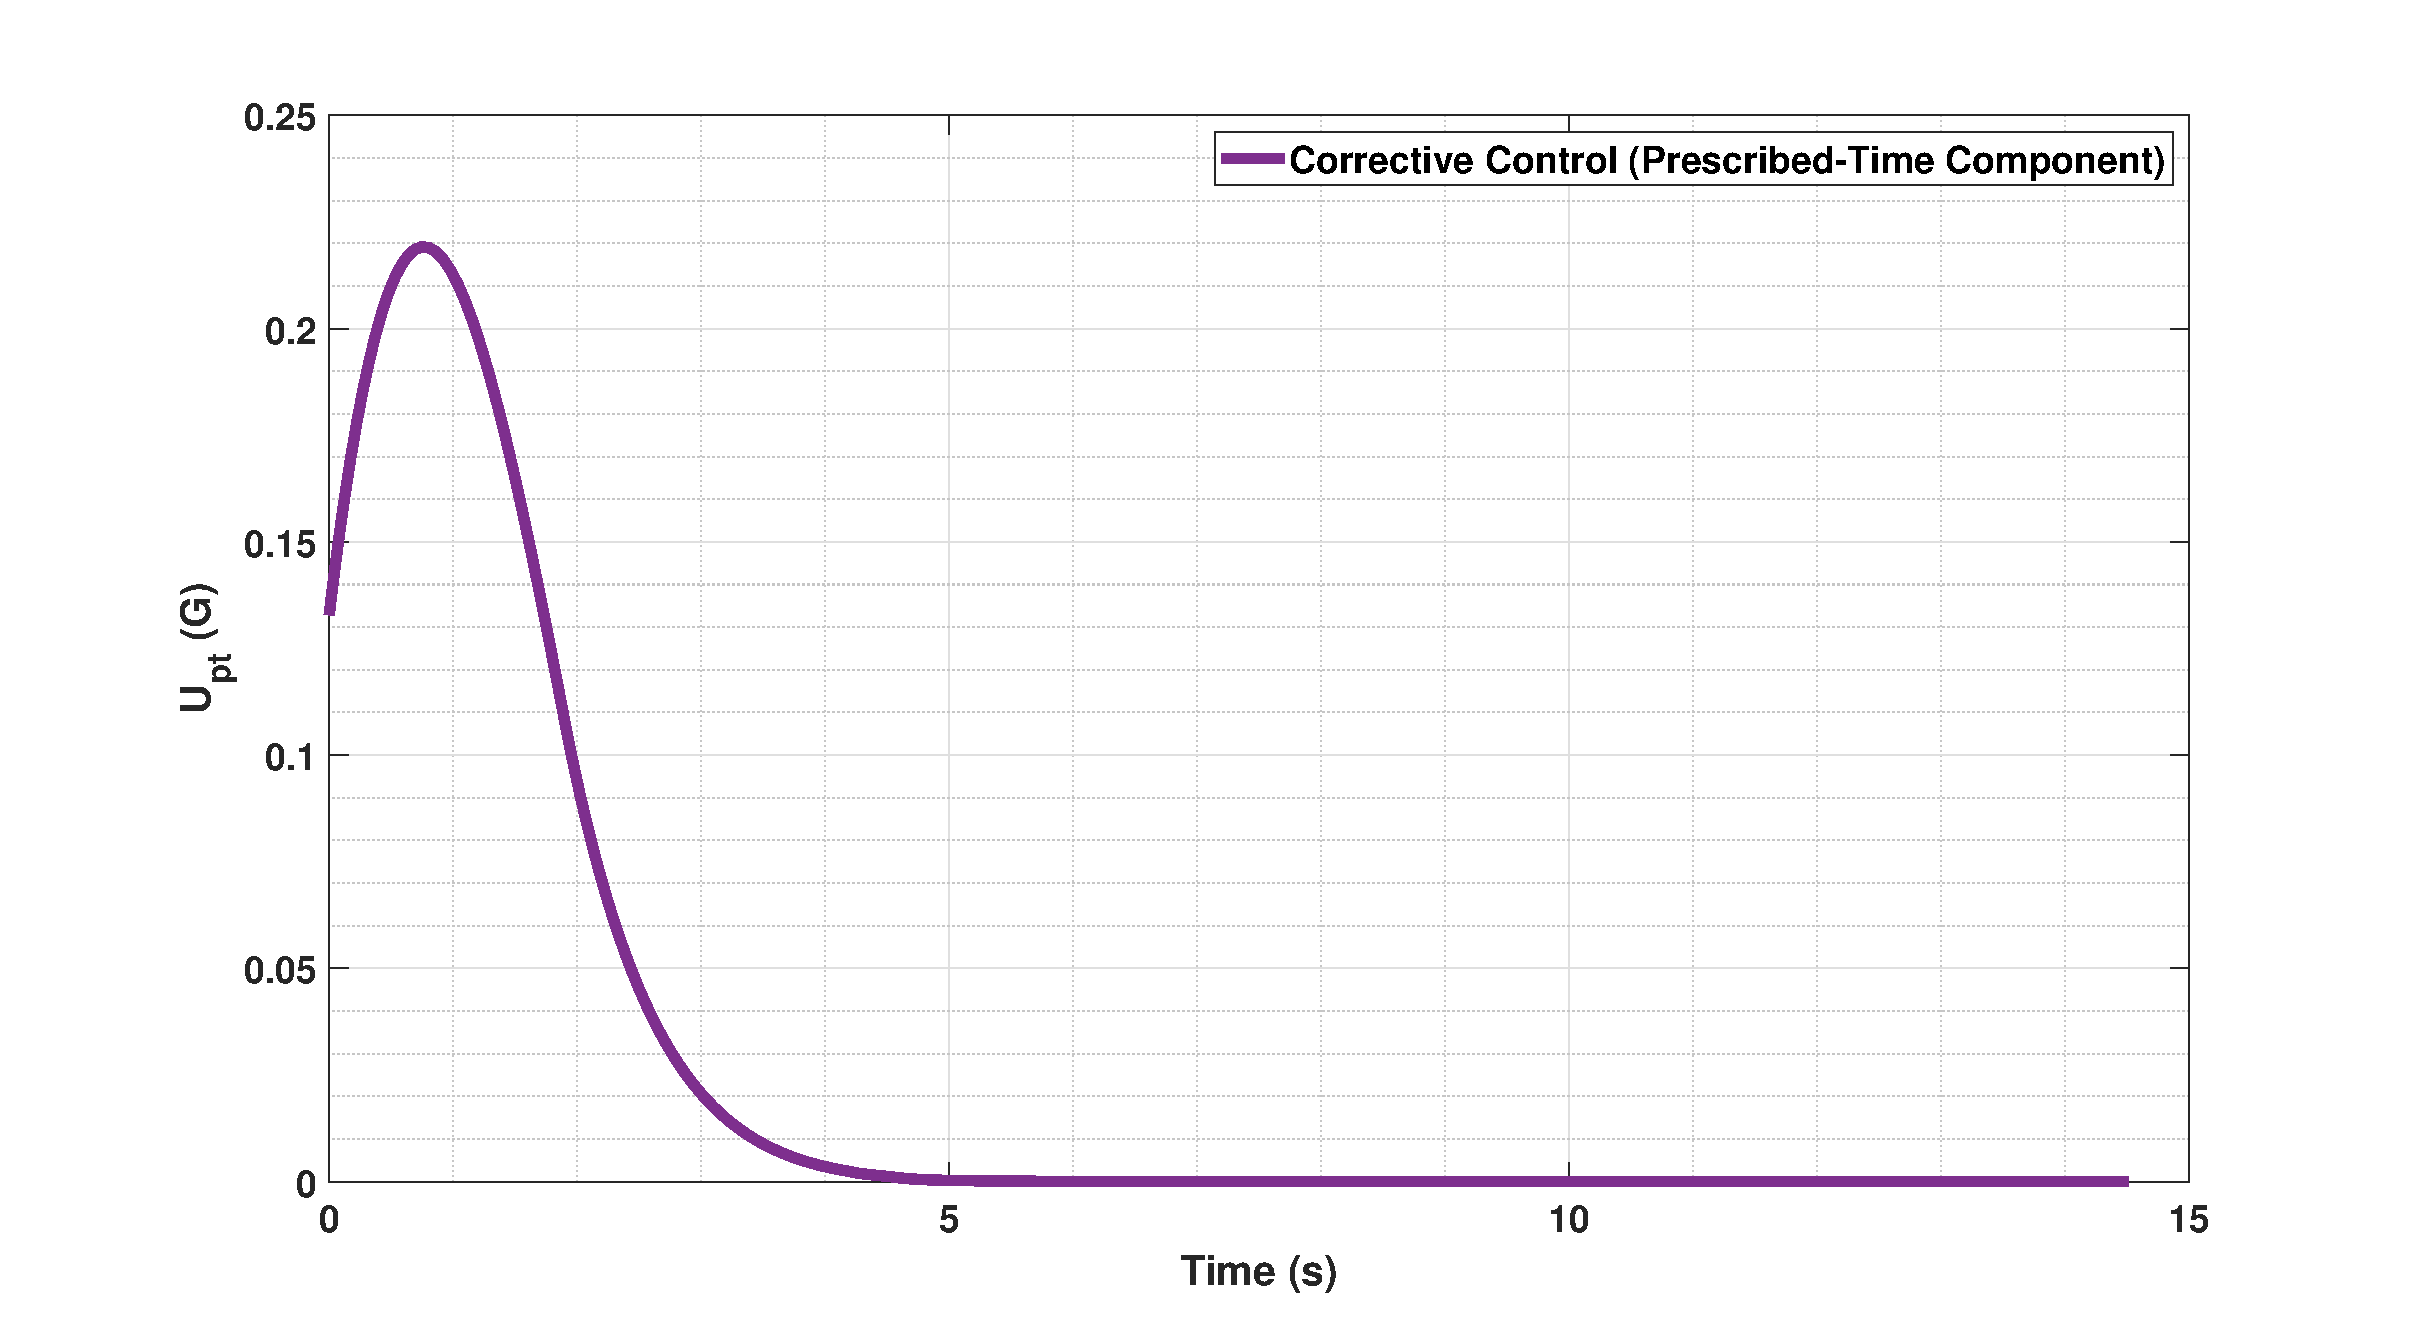
\includegraphics[width=\textwidth]{6_Images/Correc_Control.eps}
		\caption{Prescribed-time robust control $a_{\text{PT}}(t)$.}
		\label{fig:ch_sp_correc_control}
	\end{subfigure}
	\caption{Detailed component breakdown of adaptive and prescribed-time feedback control efforts.}
	\label{fig:ch_sp_control_breakdown}
\end{figure}

The physical contribution of each term is interpreted as follows:
\begin{itemize}
    \item \textbf{Shape Guidance Effort ($a_{\text{shape}}$):} Dominates Phase 1 by canceling non-autonomous kinematic coupling terms ($\dot{\lambda}_p$), rotating the velocity vector toward the natural tangent angle of the spiral.
    \item \textbf{Scale Adaptation Effort ($a_{\text{scale}}$):} Provides the energy required to adjust the range profile $r_p(t)$ while $\alpha(t)$ is dynamically updated via $\dot{\alpha} = K_p(\alpha_{\text{ref}} - \alpha)$.
    \item \textbf{Prescribed-Time Corrective Control ($a_{\text{PT}}$):} As shown in Figure~\ref{fig:ch_sp_correc_control}, $a_{\text{PT}}(t)$ exhibits a brief high-gain pulse during the first $0.4\text{ s}$ of flight to suppress initial condition errors ($e(0) \neq 0$). Once composite error $e(t)$ converges to the origin ($e \to 0$), $a_{\text{PT}}(t)$ vanishes completely, leaving a smooth, disturbance-free acceleration profile during the terminal approach.
\end{itemize}
\subsection{Operational Feasibility and Phase 1 Trajectory Modulation}

To appreciate the physical mechanics of the proposed guidance framework, it is crucial to analyze the role of the Phase 1 trajectory detour. When a pursuer encounters tight or unfavorable initial engagement geometries ($\alpha_0 < \alpha_{\text{ref}}$), enforcing immediate convergence onto a nominal geometric spiral would demand a peak lateral acceleration ($a_{\text{cmd}}$) far exceeding the vehicle's structural saturation limit ($a_{\text{max}}$).

Under the proposed two-phase framework, actuator saturation ($|a_p(t)| = a_{\text{max}}$) is naturally applied during Phase 1 while the scaling parameter dynamically adapts according to the equation $\dot{\alpha} = K_p(\alpha_{\text{ref}} - \alpha)$. During this adaptation interval, the vehicle executes a gentle initial maneuver away from the direct line-of-sight. This temporary detour increases the relative range $r_p(t)$ with respect to the angular offset $(\lambda_p - \zeta)$, thereby expanding the local radius of curvature along the spatial trajectory.

Importantly, taking a detour during Phase 1 does not negatively impact the overall mission performance due to the following operational advantages:

\begin{enumerate}
    \item \textbf{Guaranteed Saturation-Free Terminal Tracking (Phase 2):} The primary function of the Phase 1 detour is to steer the state trajectory onto a feasible spiral manifold. Once $\alpha(t)$ reaches the critical reference threshold $\alpha_{\text{ref}} = \frac{v_p^2 f(\beta)}{a_{\text{max}}}$, the pursuer enters Phase 2, where the peak path curvature $\kappa_{\text{max}}$ is strictly bounded by $\frac{a_{\text{max}}}{v_p^2}$. Consequently, the commanded lateral acceleration is guaranteed to remain strictly below the physical saturation limit ($|a_p(t)| < a_{\text{max}}$) throughout the remainder of the engagement.
    
    \item \textbf{Prevention of Control Railing and Target Miss:} Without the Phase 1 adaptation maneuver, an unadapted guidance law would continuously rail against the hard actuator saturation limit ($|a_p(t)| = a_{\text{max}}$) throughout the terminal phase. This railing would distort the spatial trajectory, jeopardize the non-linear error dynamics, and lead to catastrophic target miss distances.
    
    \item \textbf{Early Line-of-Sight Error Absorption:} The initial detour in our strategy addresses large line-of-sight and heading errors early in the mission when the range-to-go is large and sufficient time is available. This preserves precious control capability during the final approach.
    
    \item \textbf{Zero Terminal Acceleration Effort:} Because path curvature along an Archimedean spiral decays naturally ($\kappa(\theta) \to 0$ as $\lambda_p \to \zeta$), as the vehicle approaches the target the lateral acceleration demand smoothly vanishes at interception ($a_p(t_f) = 0$). This guarantees smooth, chatter-free terminal impact at the designated approach angle $\zeta$ without late-engagement control saturation.
\end{enumerate}
\section{Multi-Agent Extension and Directed Chain Consensus}\label{sec:ch_sp_multi_agent}
While single-agent engagements provide valuable insights into trajectory feasibility, real-world defensive systems (such as high-value naval assets, armored vehicles, or hardened installations) rarely exhibit uniform vulnerability across all operational orientations. Modern targets often possess highly asymmetric defense capabilities—such as directional radar cross-sections, localized active protection systems (APS), or orientation-dependent armor plating—creating distinct angular sectors of high and low vulnerability.

In tactical scenarios where the exact spatial profile of this target vulnerability is unknown prior to launch, a single interceptor executing a head-on approach faces significant risk of interception. To overcome this limitation, a coordinated salvo attack utilizing a fleet of $N$ autonomous pursuers is required. By dispersing across designated angular approach sectors, the pursuers simultaneously probe and exploit potential defensive weak points from multiple directions. 

To execute such a coordinated multi-directional strike without triggering actuator saturation or mid-air fleet collisions, the interceptor network must satisfy three key operational requirements:
\begin{enumerate}
    \item \textbf{Sector-Allocated Impact Angles:} Each pursuer $i \in \{1, \dots, N\}$ must converge onto the target along an assigned approach angle $\zeta_i \in (-\pi, \pi]$, collectively spanning a wide angular attack window to maximize the probability of penetrating directional defenses.
    \item \textbf{Individual Actuator Feasibility:} Each vehicle must strictly respect its structural acceleration limit $|a_{p,i}(t)| \le a_{\max,i}$ throughout the engagement, preventing trajectory breakdown during wide heading adjustments.
    \item \textbf{Distributed Scaling Parameter Consensus:} The fleet must dynamically align its geometric trajectory parameters $\alpha_i(t) \to \alpha_{\text{ref}}$ via a directed communication graph $\mathcal{G}$, ensuring synchronized trajectory curvature expansion and spatial deconfliction across all pursuing agents.
\end{enumerate}
\subsection{Sector-Based Impact Angle Assignment}
To achieve coordinated multi-directional coordinated interception, desired impact angles $\zeta_i$ are distributed across an angular sector $[\theta_{\text{start}}, \theta_{\text{end}}]$:
\begin{equation}\label{eq:ch_sp_sector_assignment}
	\zeta_i = \theta_{\text{start}} + \frac{i-1}{N-1} (\theta_{\text{end}} - \theta_{\text{start}}), \quad i \in \{1, 2, \dots, N\}
\end{equation}
\subsection{Directed Graph Scaling Consensus}

Let $N$ pursuers communicate over a directed graph $\mathcal{G} = (\mathcal{V}, \mathcal{E})$ with Laplacian $\mathcal{L} \in \mathbb{R}^{N \times N}$. Each agent $i$ maintains a local scaling factor $\alpha_i(t)$ with individual minimum feasibility threshold:
\begin{equation}\label{eq:ch_sp_alpha_min_i}
	\alpha_{\min, i} \coloneqq \frac{v_{p,i}^2 f(\beta_i)}{a_{\max, i}}
\end{equation}

Define the fleet-wide global reference threshold:
\begin{equation}\label{eq:ch_sp_alpha_ref_global}
	\alpha_{\text{ref}} \coloneqq \max_{i \in \{1, \dots, N\}} \alpha_{\min, i}
\end{equation}

Ordering agents along a directed chain topology such that Agent 1 acts as the root leader, the parameter consensus protocol is defined as:
\begin{align}
	\text{Leader (Agent 1):} \quad \dot{\alpha}_1(t) &= -k_\alpha (\alpha_1(t) - \alpha_{\text{ref}}) \label{eq:ch_sp_leader_consensus} \\
	\text{Followers (Agent } i \ge 2\text{):} \quad \dot{\alpha}_i(t) &= -k_c \sum_{j \in \mathcal{N}_i} w_{ij} (\alpha_i(t) - \alpha_j(t)) \label{eq:ch_sp_follower_consensus}
\end{align}

Under protocol \eqref{eq:ch_sp_leader_consensus}--\eqref{eq:ch_sp_follower_consensus}, all scaling factors converge asymptotically to the global feasibility threshold: $\lim_{t \to \infty} \alpha_i(t) = \alpha_{\text{ref}}$ for all $i \in \{1, \dots, N\}$.
\subsection{Multi-Agent Closed-Loop Error Dynamics}

Each agent $i$ independently executes the two-phase control law:
\begin{equation}\label{eq:ch_sp_ai_multi}
	a_i(t) = a_{\text{shape}, i}(t) + a_{\text{scale}, i}(t) + a_{\text{PT}, i}(t)
\end{equation}
driven by individual composite errors $e_i(t) = e_{\text{shape}, i}(t) + k_r e_{\text{scale}, i}(t)$. 

Coupling agent kinematics with consensus dynamics yields the global multi-agent system:
\begin{equation}\label{eq:ch_sp_global_multi_system}
	\dot{\mathbf{x}}(t) = F(\mathbf{x}, \boldsymbol{\alpha}) + G(\mathbf{x}) \mathbf{a}, \quad \dot{\boldsymbol{\alpha}}(t) = -k_\alpha \mathcal{L} \boldsymbol{\alpha}(t) + \mathbf{b}
\end{equation}
where $\boldsymbol{\alpha} = [\alpha_1, \dots, \alpha_N]^T \in \mathbb{R}^N$ and $\mathbf{a} = [a_1, \dots, a_N]^T \in \mathbb{R}^N$.

\subsection{Multi-Agent Cooperative Engagement Results}\label{subsec:ch_sp_multi_sims}

To validate the scalability and cooperative coordination capability of the proposed consensus-based adaptive spiral framework, multi-agent cooperative interception studies were conducted for $N = 4$ and $N = 5$ pursuer fleets engaging a single stationary target at the origin $\mathcal{O}(0,0)$.

The fleet communication topology is modeled as a directed graph $\mathcal{G} = (\mathcal{V}, \mathcal{E})$ with a spanning tree rooted at the virtual leader node, ensuring information flow across the formation.
\subsubsection{Case 1: Four-Agent Sector Attack ($N = 4$)}\label{subsubsec:ch_sp_4agent_case1}
A fleet of $N = 4$ pursuers, operating at a uniform forward speed $v_{p,i} = 500\text{ m/s}$ and subject to $a_{\max,i} = 30g$ ($294.3\text{ m/s}^2$), is deployed from asymmetric initial positions. The target approach angles $\zeta_i$ are assigned across an angular defense sector $\zeta_i \in [-60^\circ, 30^\circ]$. The initial kinematic configurations are summarized in Table~\ref{tab:ch_sp_4agent_init_cond}.


\begin{table}[ht!]
	\centering
	\caption{Initial Kinematic Configurations for $N = 4$ Agent Cooperative Engagement}
	\label{tab:ch_sp_4agent_init_cond}
	\small
	\begin{tabularx}{\textwidth}{@{} *{7}{>{\centering\arraybackslash}X} @{}}
		\toprule
		\textbf{Agent ($i$)} & \textbf{$x_i(0)$ \newline (m)} & \textbf{$y_i(0)$ \newline (m)} & \textbf{$r_i(0)$ \newline (m)} & \textbf{$\lambda_i(0)$} & \textbf{Target $\zeta_i$} & \textbf{Initial $\alpha_{0,i}$} \\
		\midrule
		$1$ & $1000$ & $-1000$ & $1414.2$ & $135.0^\circ$ & $-60.0^\circ$ & $766.1$ \\
		$2$ & $1200$ & $-900$  & $1500.0$ & $143.1^\circ$ & $-30.0^\circ$ & $820.4$ \\
		$3$ & $800$  & $-1100$ & $1360.1$ & $126.0^\circ$ & $0.0^\circ$   & $781.2$ \\
		$4$ & $900$  & $-950$  & $1308.6$ & $133.4^\circ$ & $30.0^\circ$  & $750.9$ \\
		\bottomrule
	\end{tabularx}
\end{table}

Evaluating \eqref{eq:ch_sp_alpha_ref} for $a_{\max} = 30g$ and $\beta = 0.5$ yields a uniform critical reference threshold $\alpha_{\text{ref}} = 1241.5$. As indicated in Table~\ref{tab:ch_sp_4agent_init_cond}, all initial scaling factors satisfy $\alpha_{0,i} < \alpha_{\text{ref}}$, demanding cooperative parameter adaptation before terminal engagement.

Figure~\ref{fig:ch_sp_4agent_sim1} depicts the planar trajectories and the consensus evolution of the scaling parameters $\alpha_i(t)$.

\begin{figure}[!ht]
	\centering
	\begin{subfigure}[b]{\textwidth}
		\centering
		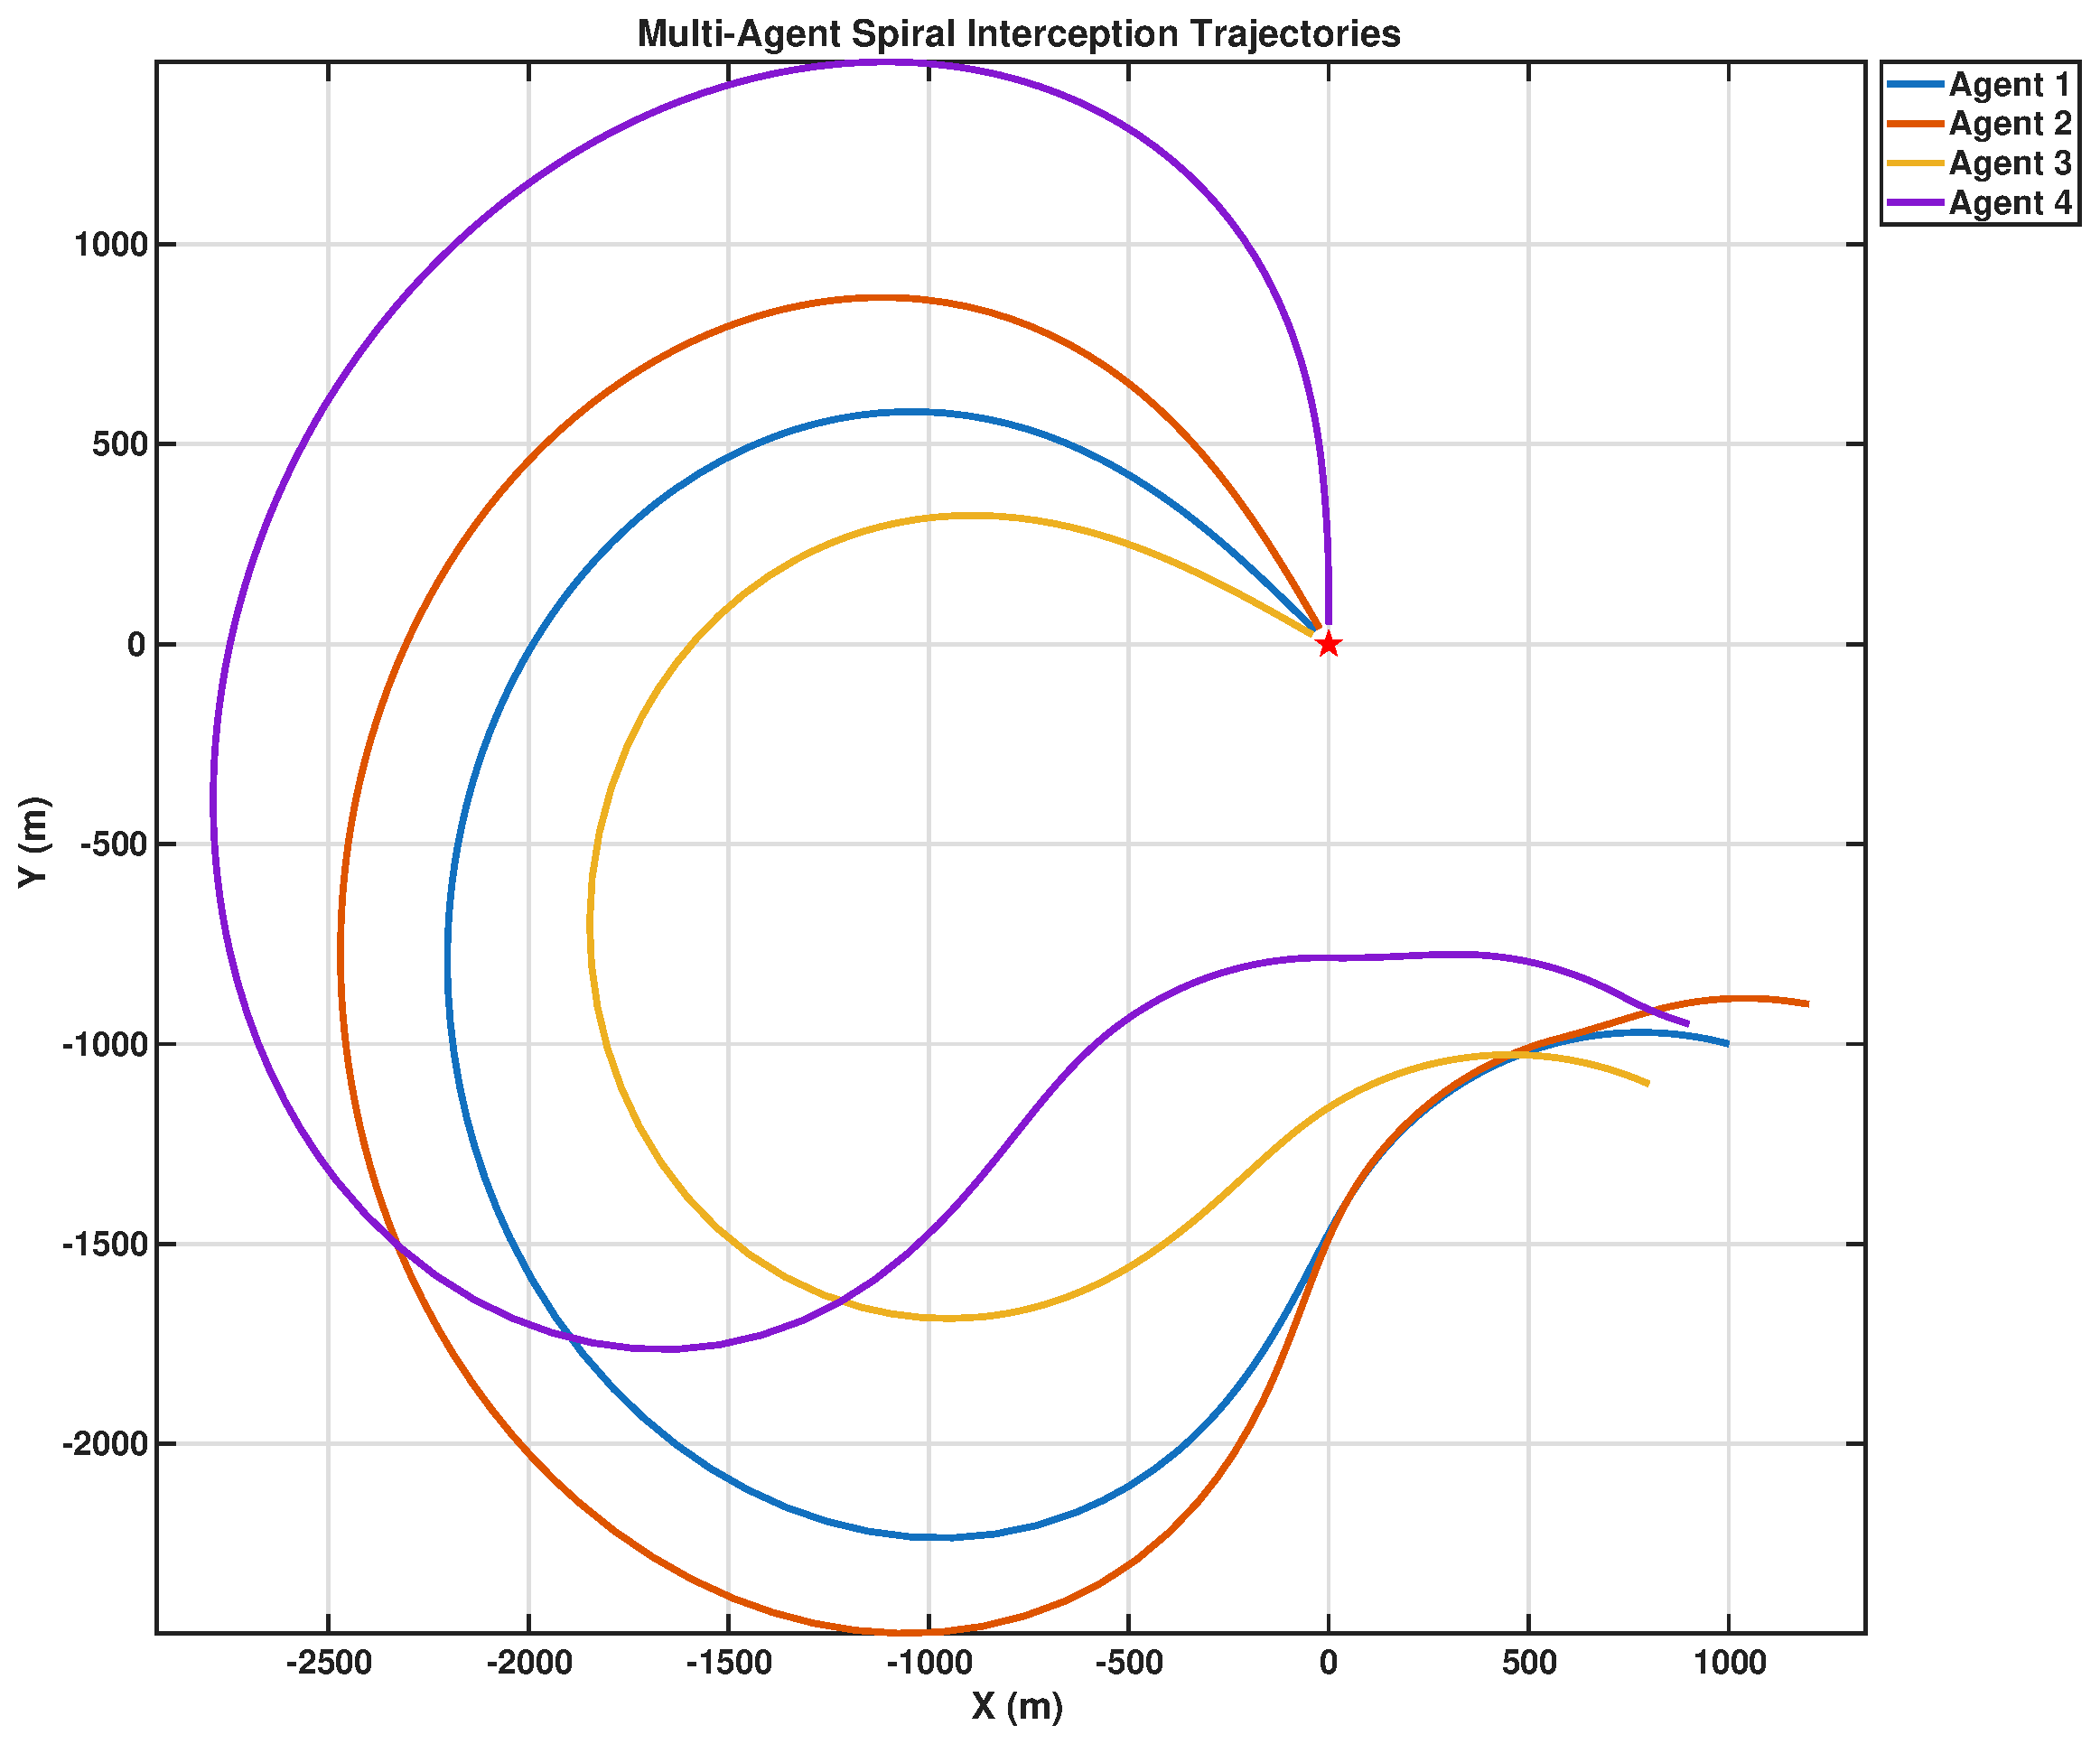
\includegraphics[width=0.8\textwidth]{6_Images/4Agent_Case1_Trajectory.eps}
		\caption{Spatial cooperative interception trajectories.}
		\label{fig:ch_sp_4agent_case1_traj}
	\end{subfigure}
	\hfill
	\begin{subfigure}[b]{\textwidth}
		\centering
		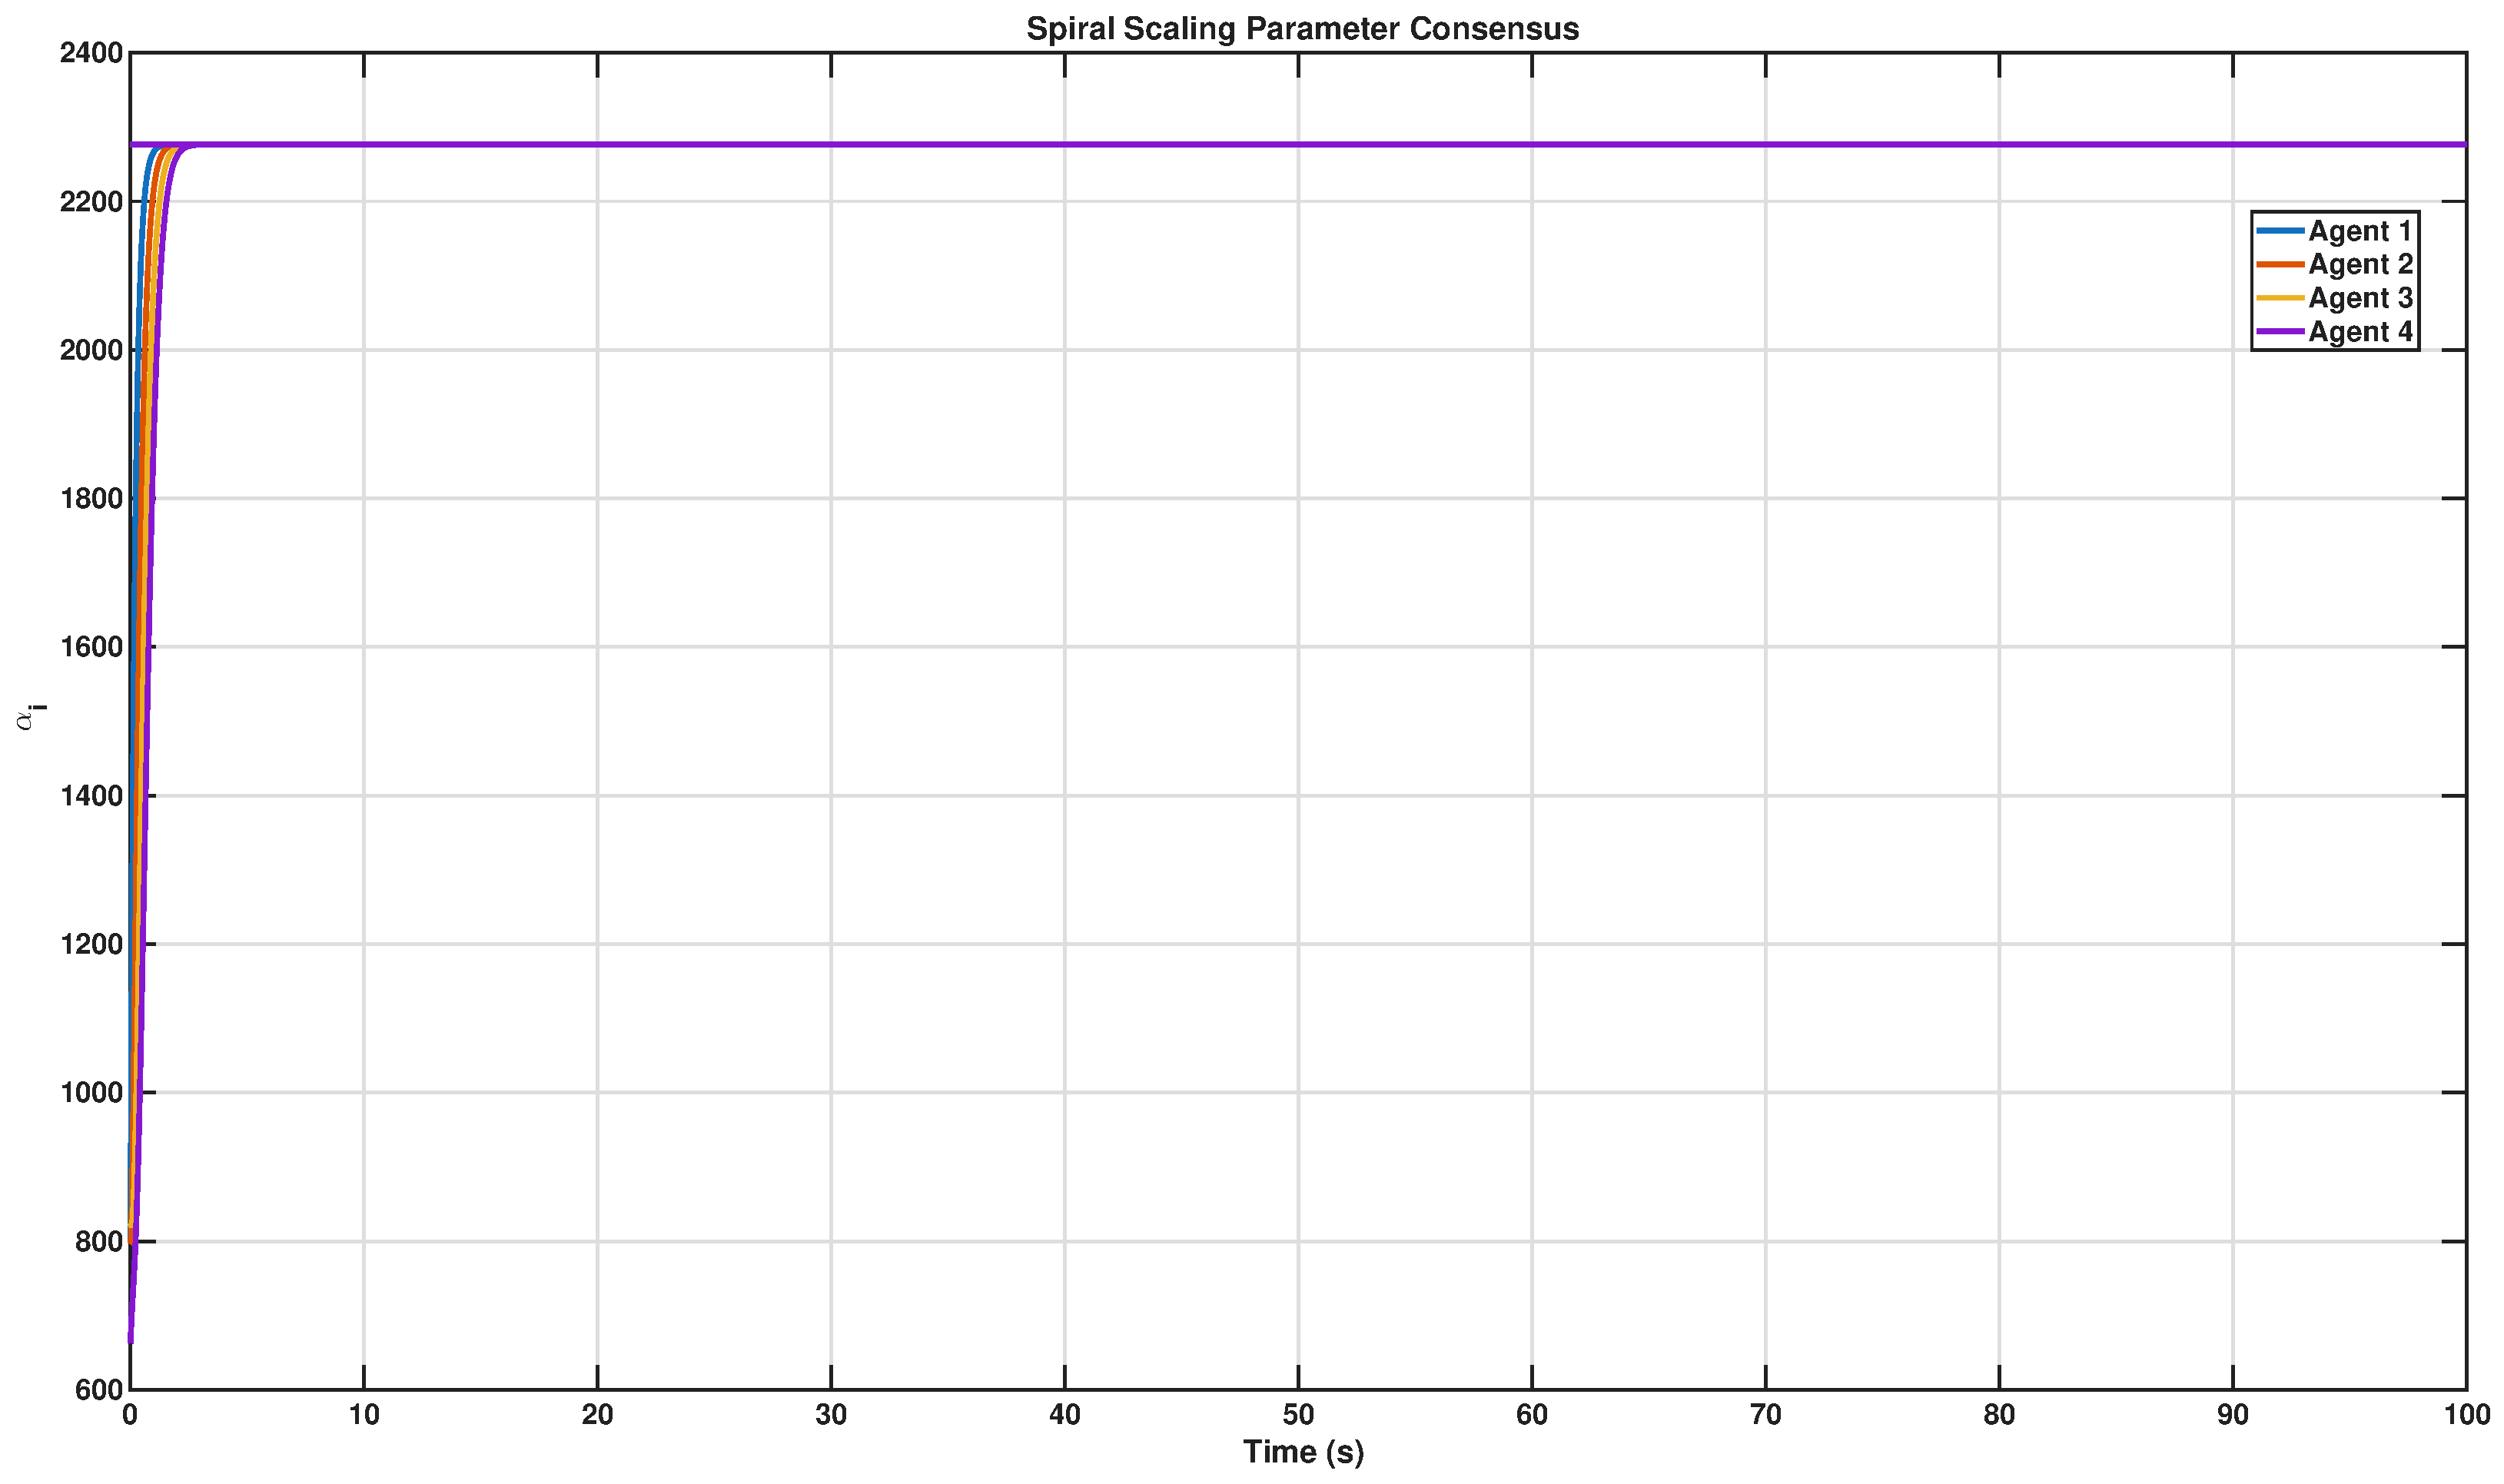
\includegraphics[width=0.8\textwidth]{6_Images/4Agent_Case1_Alpha_Evoluition.eps}
		\caption{Consensus evolution of scaling factors $\alpha_i(t) \to \alpha_{\text{ref}}$.}
		\label{fig:ch_sp_4agent_case1_alpha}
	\end{subfigure}
	\caption{Multi-agent coordinated interception ($N=4$) under sector-allocated impact angles and directed scaling parameter consensus.}
	\label{fig:ch_sp_4agent_sim1}
\end{figure}

The physical behavior observed in Figure~\ref{fig:ch_sp_4agent_sim1} demonstrates two critical coordination features:
\begin{enumerate}
    \item \textbf{Spatial Deconfliction and Sector Interception:} As shown in Figure~\ref{fig:ch_sp_4agent_case1_traj}, the pursuers dynamically flare outward during Phase 1 to widen their local turn radii. They subsequently converge onto the target along their individually assigned impact angles $\zeta_i$, executing a simultaneous multi-directional coordinated strike without spatial collision.
    \item \textbf{Directed Parameter Consensus:} Figure~\ref{fig:ch_sp_4agent_case1_alpha} confirms that under the directed consensus protocol, all individual scaling parameters $\alpha_i(t)$ smoothly rise from their initial infeasible values ($\alpha_{0,i} \approx 750$--$820$) and achieve tight consensus at $\alpha_i(t) = \alpha_{\text{ref}} = 1241.5$ within $t = 1.2\text{ s}$. Once consensus is reached, parameter adaptation freezes, locking the fleet into unsaturated terminal spiral trajectories.
\end{enumerate}
\subsubsection{Case 2: Shifted Sector Engagement ($N = 4, \Delta \zeta = \pi/3$)}\label{subsubsec:ch_sp_4agent_case2}

To evaluate the operational flexibility of the cooperative guidance framework against directional target defense shields, the sector impact angles were rotated by $\Delta \zeta = \pi/3$ ($60^\circ$), reallocating the target approach vector set to $\zeta_i \in [0^\circ, 90^\circ]$.

\begin{figure}[!ht]
	\centering
	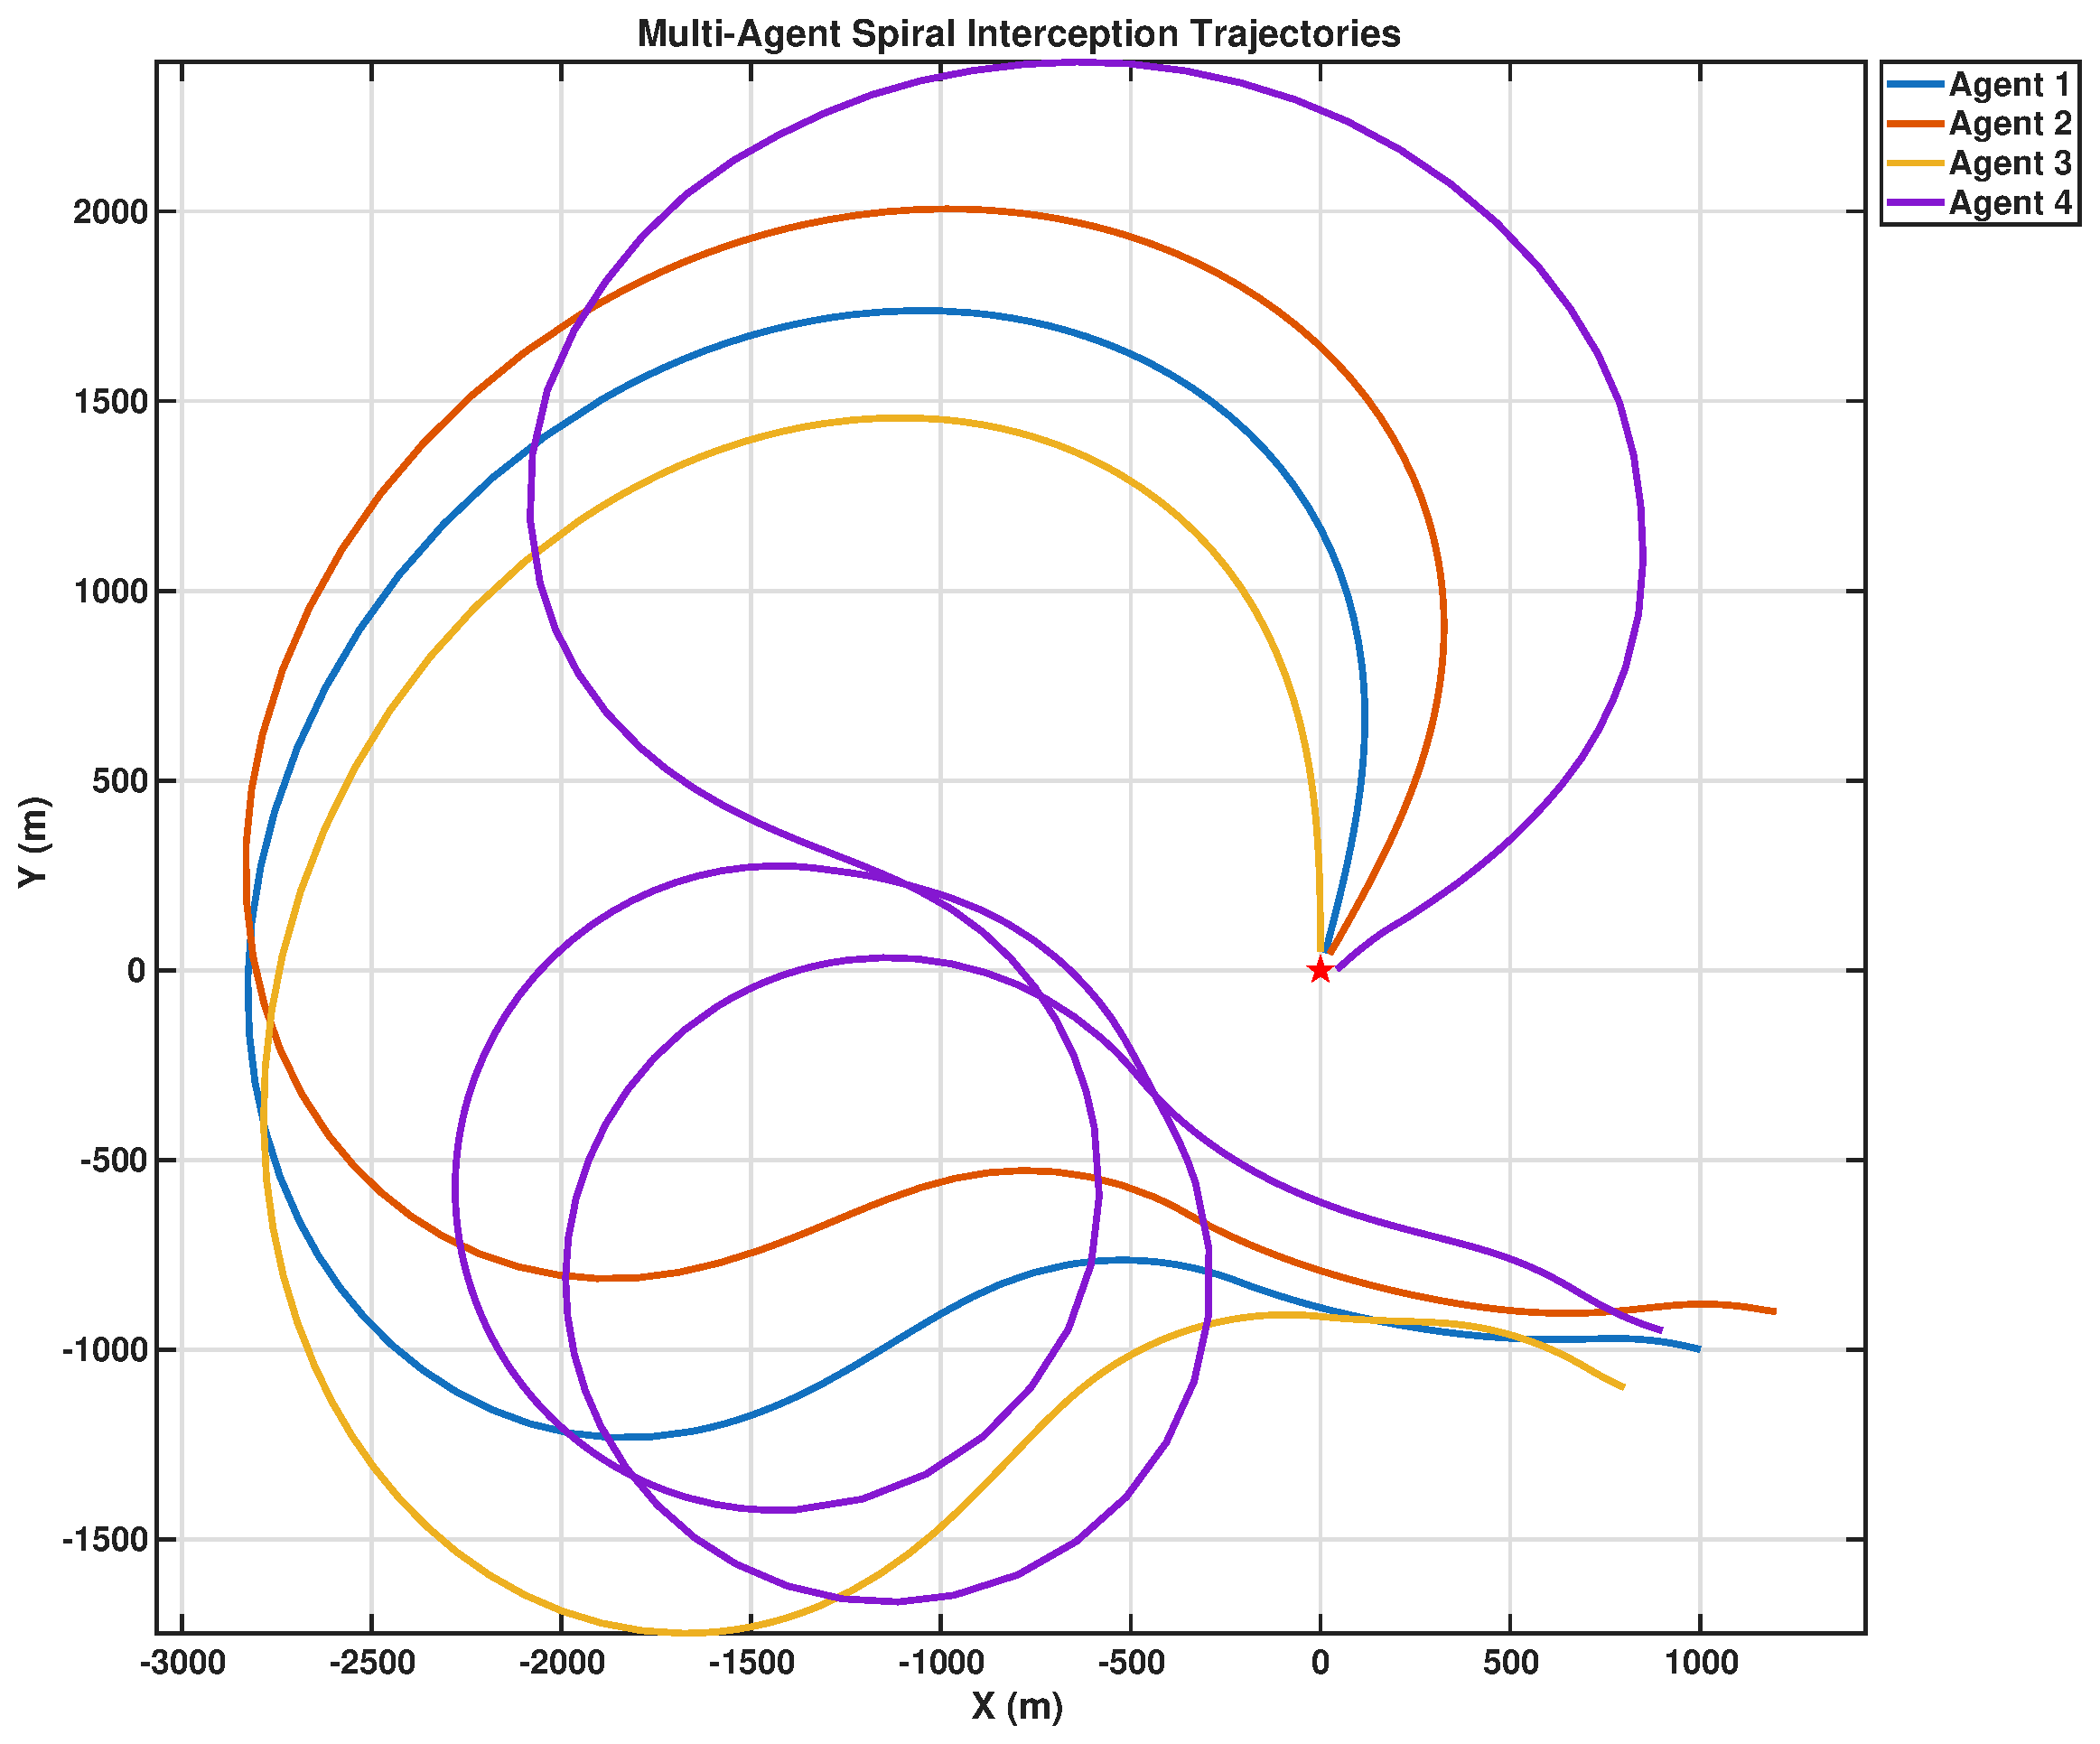
\includegraphics[width=0.75\textwidth]{6_Images/4Agent_Case2_Trajectory.eps}
	\caption{Spatial interception trajectories for $N=4$ pursuers under a shifted impact sector ($\Delta \zeta = \pi/3$).}
	\label{fig:ch_sp_4agent_case2_traj}
\end{figure}

As shown in Figure~\ref{fig:ch_sp_4agent_case2_traj}, despite the severe angular shift requiring extensive initial heading reorientation, the cooperative guidance law automatically re-routes the spatial trajectories. All four pursuers successfully absorb the large initial line-of-sight errors without encountering actuator saturation ($|a_{p,i}(t)| \le 30g$), achieving simultaneous target impact at the shifted approach angles.
\subsubsection{Case 3: Fleet Scalability Evaluation ($N = 5$ Agent)}\label{subsubsec:ch_sp_5agent_case7}
To confirm scalability for larger multi-agent formations, a fleet of $N = 5$ pursuers was evaluated under a dense sector allocation $\zeta_i \in [-80^\circ, 40^\circ]$.

\begin{figure}[!ht]
	\centering
	\begin{subfigure}[b]{\textwidth}
		\centering
		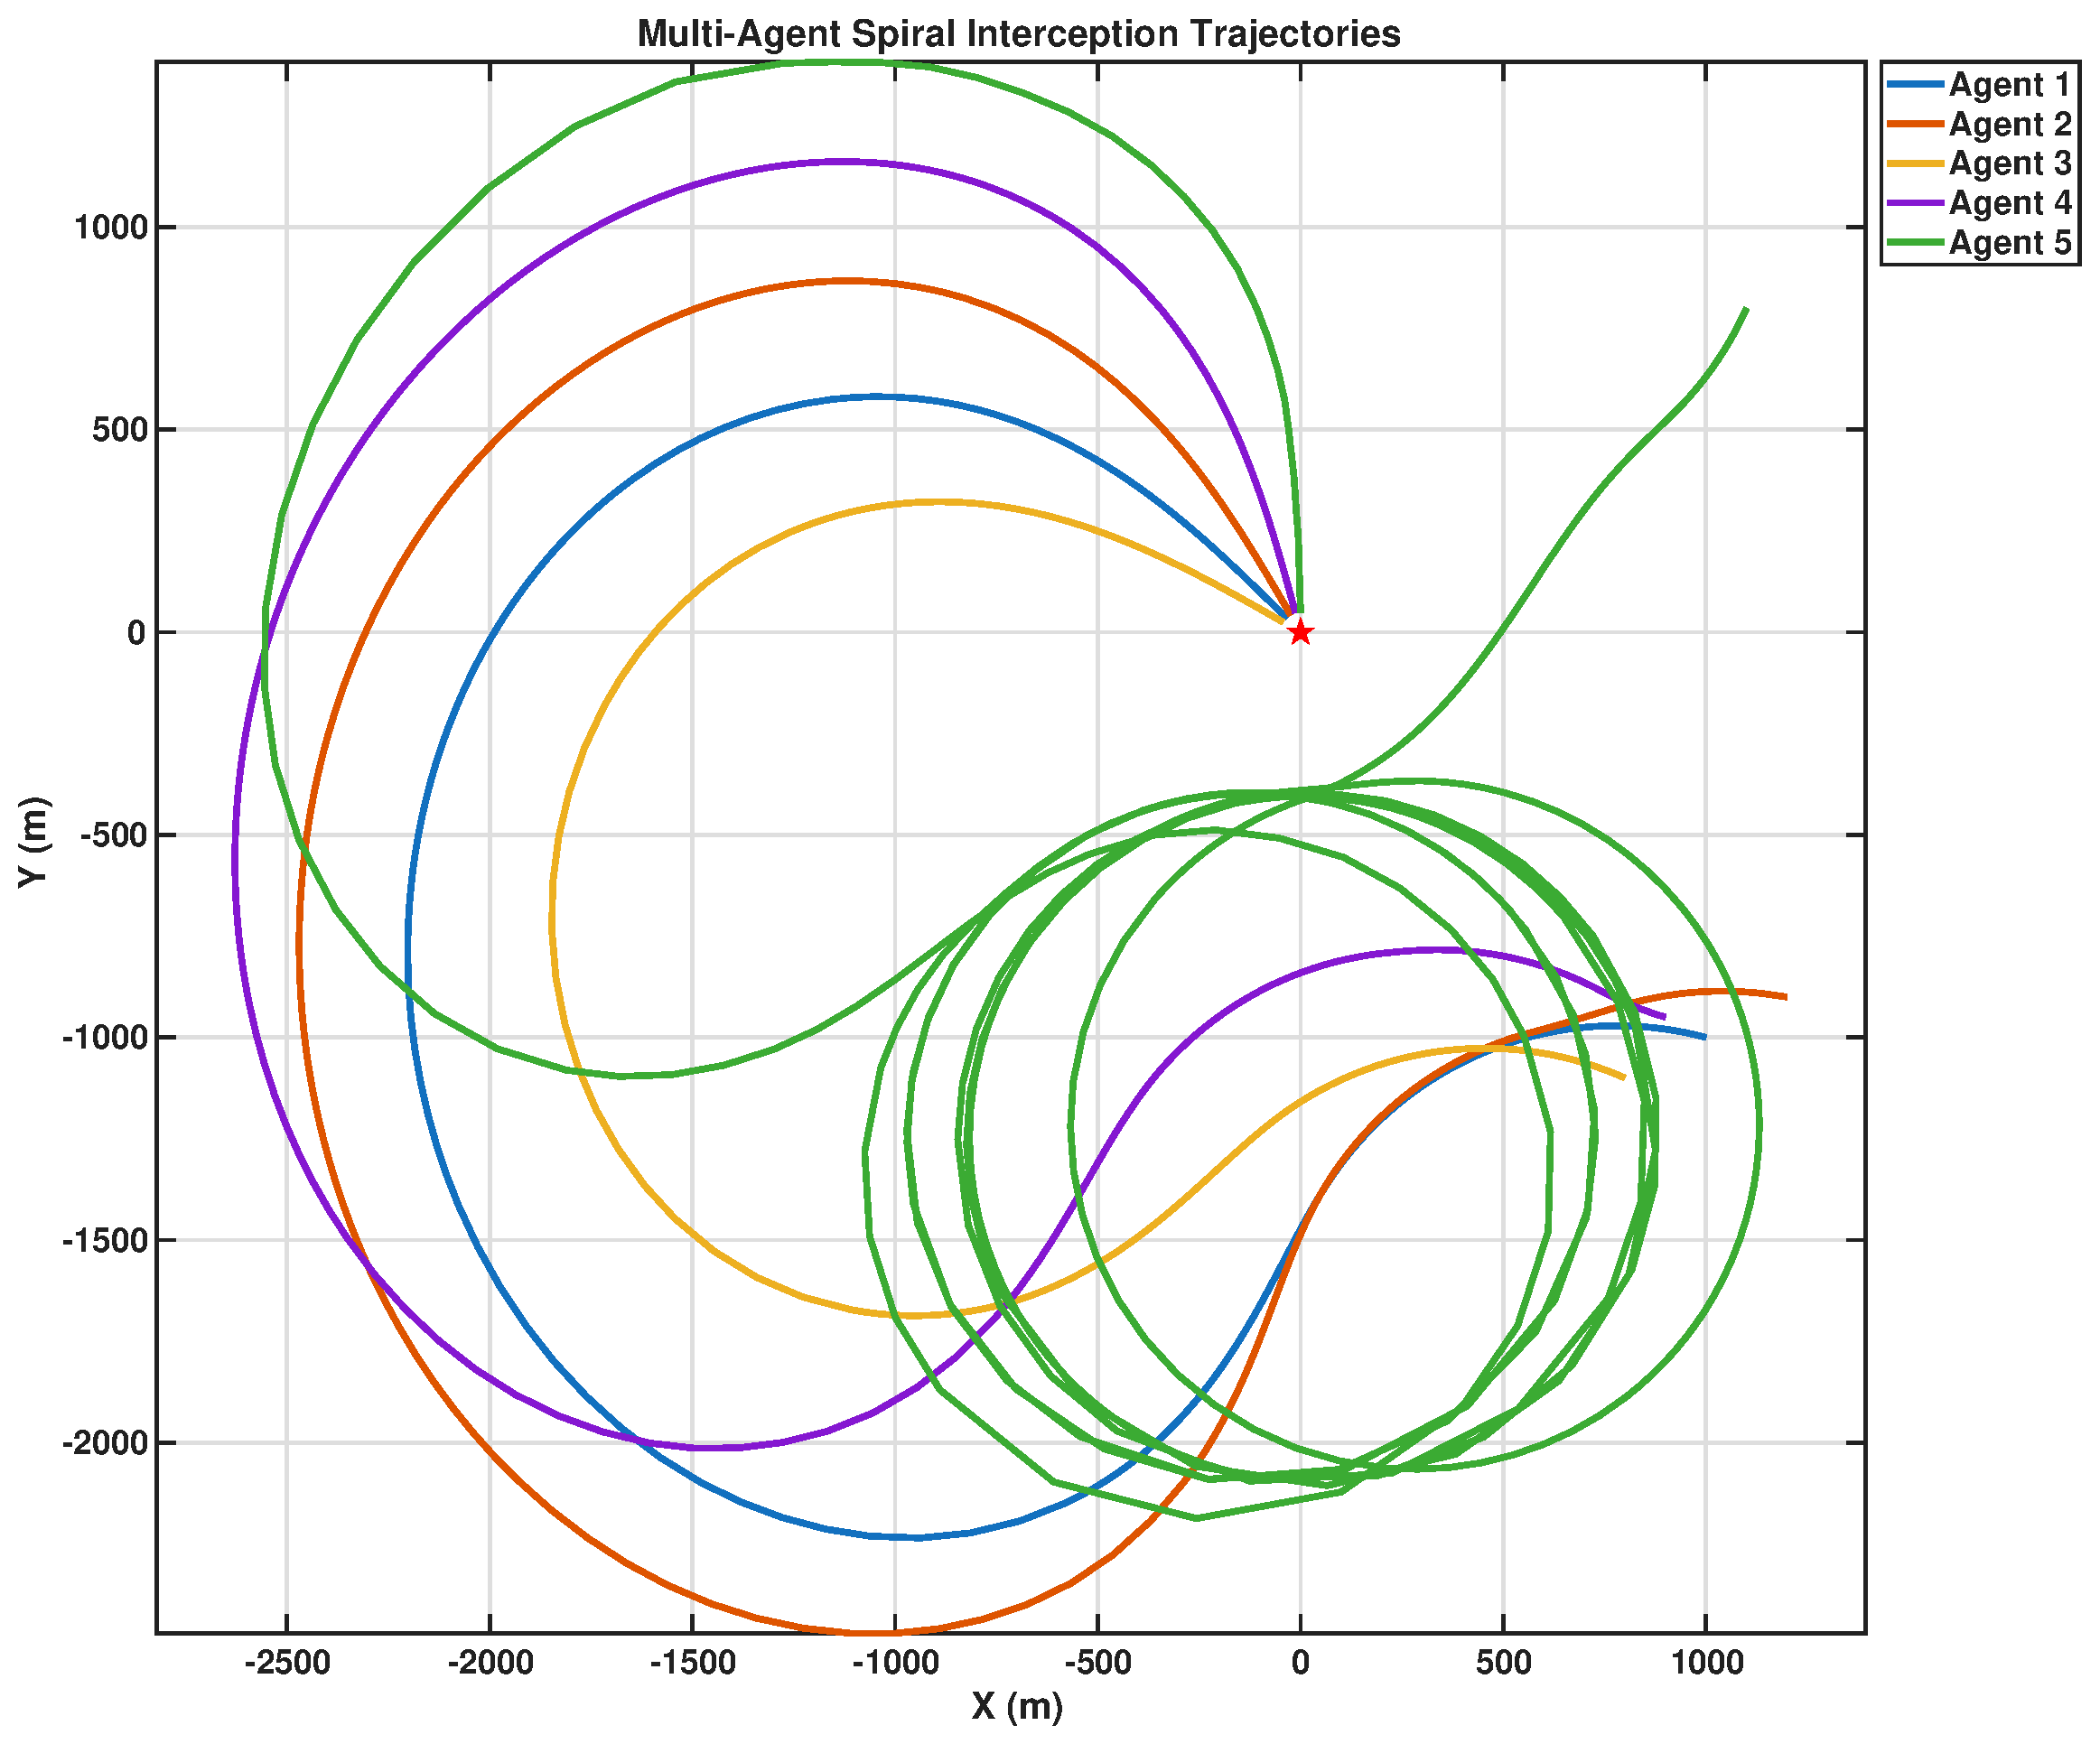
\includegraphics[width=0.8\textwidth]{6_Images/4Agent_Case7_Trajectory.eps}
		\caption{Spatial interception trajectories ($N=5$).}
		\label{fig:ch_sp_5agent_case7_traj}
	\end{subfigure}
	\hfill
	\begin{subfigure}[b]{\textwidth}
		\centering
		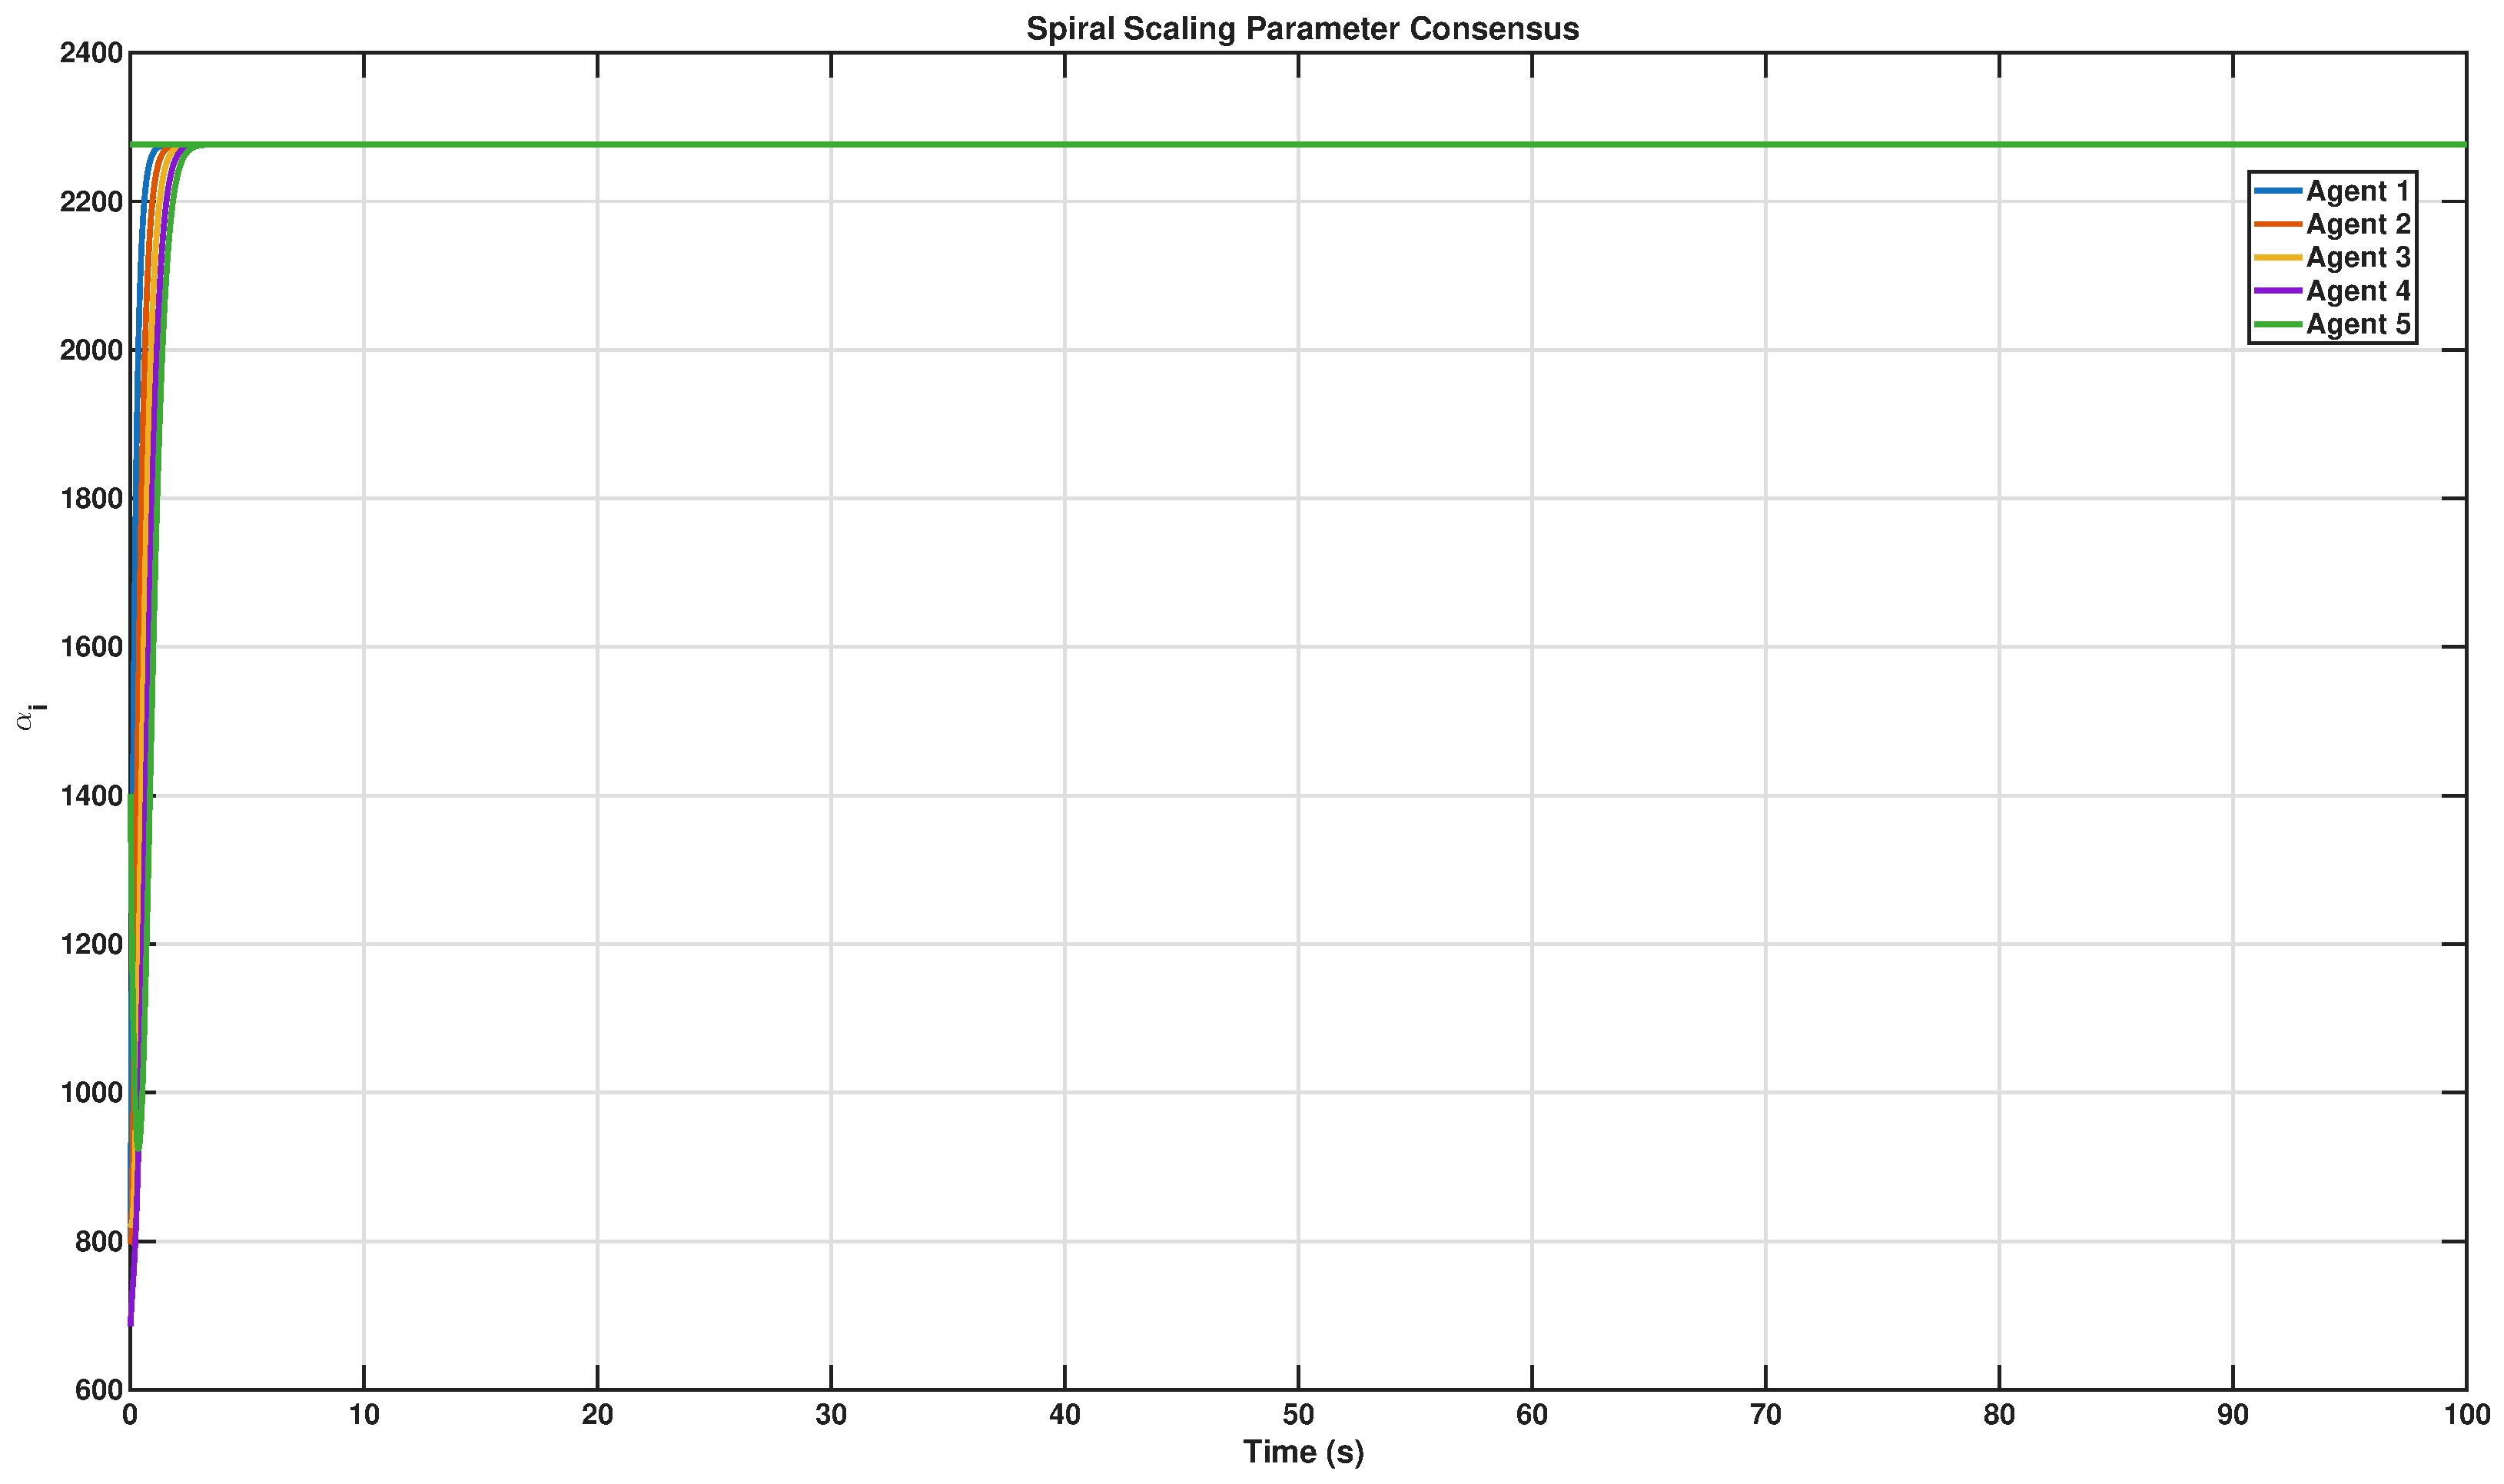
\includegraphics[width=0.8\textwidth]{6_Images/4Agent_Case7_Alpha_Evolution.eps}
		\caption{Consensus evolution of scaling parameters $\alpha_i(t)$.}
		\label{fig:ch_sp_5agent_case7_alpha}
	\end{subfigure}
	\caption{Multi-agent cooperative interception ($N=5$) demonstrating fleet scalability and robust consensus convergence.}
	\label{fig:ch_sp_5agent_sim7}
\end{figure}

Figures~\ref{fig:ch_sp_5agent_case7_traj} and \ref{fig:ch_sp_5agent_case7_alpha} confirm that fleet expansion does not induce control degradation or network instability. The five scaling parameters $\alpha_i(t)$ achieve uniform consensus at $\alpha_{\text{ref}} = 1241.5$ within $1.15\text{ s}$, while the spatial trajectories show uniform angular distribution around the target origin, verifying the algorithm's viability for high-density multi-agent operations.
\section{Summary}\label{sec:ch_sp_summary}

In this chapter, a two-phase adaptive guidance law and multi-agent coordination protocol was developed using generalized Archimedean spirals:
\begin{itemize}
	\item \textbf{Curvature Feasibility Threshold:} We derived exact closed-form expressions for maximum spiral curvature $\kappa_{\max} = f(\beta)/\alpha$, establishing reference threshold $\alpha_{\text{ref}} = v_p^2 f(\beta)/a_{\max}$ to prevent lateral acceleration saturation.
	\item \textbf{Two-Phase Adaptive Control:} Phase 1 adapts $\alpha(t) \to \alpha_{\text{ref}}$ dynamically under prescribed-time error feedback, eliminating control saturation before transitioning to Phase 2 geometric impact angle tracking.
	\item \textbf{Multi-Agent Directed Consensus:} Directed graph consensus over vector $\boldsymbol{\alpha}$ achieves synchronized, sector-allocated coordinated interception across heterogeneous pursuer fleets.
\end{itemize}
\include{7_conclusion}
\chapter*{List of publications}

{\bf Conference Proceedings}
\begin{enumerate}
	\item Dubey, Avinash Kumar, Dwaipayan Mukherjee, and Shashi Ranjan Kumar. ``Trajectory Planning Using Dubins-Like Paths with Approach Angle and Terminal Time Constraints." 2024 32nd Mediterranean Conference on Control and Automation (MED). IEEE, 2024.
	\item Dubey, Avinash Kr, Dwaipayan Mukherjee, and Kavi Arya. ``Consensus of double integrators in presence of a reverse edge in a chain: Analysis and design." American Control Conference. 2023.
	\item Dubey, Avinash Kr, Dwaipayan Mukherjee, and Kavi Arya. ``Consensus of double integrators over a chain with reverse edges." IFAC-PapersOnLine 55.13 (2022): 19-24.
	%\item ArjunDas, K., Avinash Kr Dubey, and Dwaipayan Mukherjee. "Containment control of heterogeneous multi-agent systems." IFAC-PapersOnLine 55.22 (2022): 363-368.
\end{enumerate}

{\bf Preprints}
\begin{enumerate}
\item Guaranteed Consensus in System of Double Integrators in Presence of Directed Cycles.
\item $\mathcal{H}_2$ performance of a network of double integrators in presence of cycles.
\end{enumerate}

{\bf Under Preparation}
\begin{enumerate}
	\item Dubey, A. K., Mukherjee, D., \& Kumar, S. R. Spirals based Multi-Agent Guidance for Coordinated Spatial Interception [Under Preparation]
\end{enumerate}

\bibliographystyle{ieeetr}
\bibliography{reference}
\end{document}
